\documentclass[a4paper]{article}
%\usepackage[utf8]{inputenc}
\usepackage[spanish, es-tabla, es-noshorthands]{babel}
\usepackage[table,xcdraw,dvipsnames]{xcolor}
\usepackage[a4paper, footnotesep=1.25cm, headheight=1.25cm, top=2.54cm, left=2.54cm,
 bottom=2.54cm, right=2.54cm]{geometry}
%\geometry{showframe}
 \usepackage[normalem]{ulem}
 \useunder{\uline}{\ul}{}

%VERIFICAR EL HEAD Y EL FOOT EN
%https://ctan.dcc.uchile.cl/macros/latex/contrib/geometry/geometry.pdf

%Paquetes varios:
\usepackage{verbatimbox}

%\usepackage{wrapfig}			%Wrap figure in text
\usepackage[export]{adjustbox}	%Move images
\usepackage{changepage}			%Move tables
\usepackage{todonotes}

\usepackage{tikz}
\usepackage{amsmath}
\usepackage{amsfonts}
\usepackage{amssymb}
\usepackage{float}
\usepackage[graphicx]{realboxes}
\usepackage{caption}
\usepackage{subcaption}
\usepackage{multicol}
\usepackage{multirow}
\setlength{\doublerulesep}{\arrayrulewidth}
%\usepackage{booktabs}

\usepackage{array}
\newcolumntype{C}[1]{>{\centering\let\newline\\\arraybackslash\hspace{0pt}}m{#1}}
%\usepackage[american]{circuitikz}
\usetikzlibrary{calc}
\usepackage{fancyhdr}
\usepackage{units} 

\usepackage{colortbl}
%\usepackage{sectsty}
%\usepackage{unicode-math}

%FONTS (IMPORTANTE): Compilar en XeLaTex o LuaLaTeX
\usepackage{anyfontsize}	%Font size
\usepackage{fontspec}		%Font type
%Si sigue sin andar comentar \usepackage[utf8]{inputenc}
%https://ctan.dcc.uchile.cl/macros/unicodetex/latex/fontspec/fontspec.pdf
%https://www.overleaf.com/learn/latex/XeLaTeX

%Path para imagenes para trabajar en subarchivos
\graphicspath{{../Resumen/}{../Referencias/}{../Apendice/}{../Descripción de la Empresa/}{../Tareas del Alumno/}{../Conclusiones/}{../Herramientas Empleadas/}}

%Definiciones de nuevos comandos y colores
%COLORES:
\definecolor{AzulFoot}{rgb}{0.682,0.809,0.926}	%RGB	%{174,206,235}
\definecolor{AzulInfo}{rgb}{0.180,0.455,0.710}	%RGB	%{46,116,181}
\definecolor{AzulTable}{rgb}{0.302,0.507,0.871}	%RGB	%{68,114,196}
\definecolor{PName}{rgb}{0.353,0.353,0.353}		%RGB	%{90,90,90}
\definecolor{mygreen}{rgb}{28,172,0} % color values Red, Green, Blue
\definecolor{mylilas}{rgb}{170,55,241}

%Change Font Size

% #1 = size, #2 = text
\newcommand{\setparagraphsize}[2]{{\fontsize{#1}{6}\selectfont#2 \par}}		%Cambia el size de todo el parrafo
\newcommand{\setlinesize}[2]{{\fontsize{#1}{6}\selectfont#2}}				%Cambia el font de una oración

%IMAGE IN TABLE:			%Ejemplo: \includeintable{.3}{ImagenesFactibilidad/pend}
\renewcommand\fbox{\fcolorbox{white}{white}}
\setlength{\fboxrule}{0pt}	%padding thickness
\setlength{\fboxsep}{4pt}	%border thickness
\newcommand{\includeintable}[2]{	
	\fbox{
		\begin{minipage}{#1\textwidth}
        	\includegraphics[width=\linewidth]{#2}
    	\end{minipage}
	}
}

%LINK IN REF
\newcommand{\reflink}[1]{		%LINK
	\href{#1}{#1}
}

%NOTAS:
\newcommand{\note}[1]{		%RED BIG NOTE (TODO)
	\begin{center}
		\huge{ \textcolor{red}{#1} }
	\end{center}
}

\newcommand{\lnote}[1]{{\fontsize{14}{6}\selectfont\textcolor{green}{#1}}}	%Notas pequeñas

\newcommand{\observacion}[2]{  \ifnumequal{1}{#1}{ { \todo[inline,backgroundcolor=red!25,bordercolor=red!100]{\textbf{Observación: #2}} } }{  }  }

\newcommand{\red}[1]{\textcolor{red}{#1}}

\newcommand{\TBD}{\textcolor{red}{(TBD) }}
\newcommand{\tbd}{\textcolor{red}{(TBD) }}

\newcommand{\TBC}{\textcolor{red}{(TBC) }}
\newcommand{\tbc}{\textcolor{red}{(TBC) }}

\newcommand{\quotes}[1]{``#1''}
\newcommand{\q}[1]{``#1''}

\newcommand{\ip}{192.168.0.10:1880}
\newcommand{\ipadmin}{192.168.0.10:1880/admin}

% Comandos para agregar elementos en tablas de acronimos y definiciones
\newcommand{\addacronym}[2]{\textbf{#1} & \begin{tabular}[l]{@{}l@{}}#2\end{tabular} \\ \hline}

% tabItem
\newcommand{\tabitem}{~~\llap{\textbullet}~~}


\usepackage{hyperref}
\hypersetup{
    colorlinks=true,
    linkcolor=black,
    filecolor=magenta,      
    urlcolor=AzulInfo,
    citecolor=AzulInfo,    
}

%Configuración del header y del footer:
\usepackage{etoolbox}
\pagestyle{fancy}
\fancyhf{}
\rfoot{\thepage}
\renewcommand{\footrulewidth}{4pt}
\renewcommand{\headrulewidth}{0pt}
\patchcmd{\footrule}{\hrule}{\color{AzulFoot}\hrule}{}{}

%Código en el informe
%% IMPORTANTE:
% Verificar que esté \usepackage[dvipsnames]{xcolor}

%\usepackage{listingsutf8}
\usepackage{listings}

\renewcommand{\lstlistingname}{Código}

%LSTSET: Pone un recuadro y contador de linea en el codigo
\newcommand{\boxstyle}{
	\lstset{
		basicstyle=\sffamily\color{black},
		frame=single,
		numbers=left,
		numbersep=5pt,
		numberstyle=\color{gray},
		showspaces=false,
		showstringspaces=false
	}
}

\newcommand{\defaultstyle}{
	\lstset{
		basicstyle=\sffamily\color{white},
		frame=none,
		numbers=none,
		showspaces=true,
		showstringspaces=true
	}
}

\lstdefinelanguage{Kotlin}{
  captionpos=b,
  comment=[l]{//},
  commentstyle={\color{gray}\ttfamily},
  emph={filter, first, firstOrNull, forEach, lazy, map, mapNotNull, println},
  emphstyle={\color{OrangeRed}},
  identifierstyle=\color{black},
  keywords={!in, !is, abstract, actual, annotation, as, as?, break, by, catch, class, companion, const, constructor, continue, crossinline, data, delegate, do, dynamic, else, enum, expect, external, false, field, file, final, finally, for, fun, get, if, import, in, infix, init, inline, inner, interface, internal, is, lateinit, noinline, null, object, open, operator, out, override, package, param, private, property, protected, public, receiveris, reified, return, return@, sealed, set, setparam, super, suspend, tailrec, this, throw, true, try, typealias, typeof, val, var, vararg, when, where, while},
  keywordstyle={\color{NavyBlue}\bfseries},
  morecomment=[s]{/*}{*/},
  morestring=[b]",
  morestring=[s]{"""*}{*"""},
  ndkeywords={@Deprecated, @JvmField, @JvmName, @JvmOverloads, @JvmStatic, @JvmSynthetic, Array, Byte, Double, Float, Int, Integer, Iterable, Long, Runnable, Short, String, Any, Unit, Nothing},
  ndkeywordstyle={\color{BurntOrange}\bfseries},
  sensitive=true,
  stringstyle={\color{ForestGreen}\ttfamily},
}

\lstdefinelanguage{Swift}
{
  morekeywords={
    open,catch,@escaping,nil,throws,func,if,then,else,for,in,while,do,switch,case,default,where,break,continue,fallthrough,return,
    typealias,struct,class,enum,protocol,var,func,let,get,set,willSet,didSet,inout,init,deinit,extension,
    subscript,prefix,operator,infix,postfix,precedence,associativity,left,right,none,convenience,dynamic,
    final,lazy,mutating,nonmutating,optional,override,required,static,unowned,safe,weak,internal,
    private,public,is,as,self,unsafe,dynamicType,true,false,nil,Type,Protocol,
  },
  morecomment=[l]{//}, % l is for line comment
  morecomment=[s]{/*}{*/}, % s is for start and end delimiter
  morestring=[b]", % defines that strings are enclosed in double quotes
  breaklines=true,
  escapeinside={\%*}{*)},
  numbers=left,
  captionpos=b,
  breakatwhitespace=true,
  basicstyle=\linespread{1.0}\ttfamily, % https://tex.stackexchange.com/a/102728/129441
}

\definecolor{keyword}{HTML}{BA2CA3}
\definecolor{string}{HTML}{D12F1B}
\definecolor{comment}{HTML}{008400}

\newcommand{\swiftstyle}{
	\lstset{
  		language=Swift,
  		inputencoding=utf8x,
		extendedchars=\true,
	  	basicstyle=\ttfamily,
	  	showstringspaces=false, % lets spaces in strings appear as real spaces
  		columns=fixed,
  		keepspaces=true,
  		keywordstyle=\color{keyword},
  		stringstyle=\color{string},
  		commentstyle=\color{comment}
	}
}


%Como usarlo:

%\begin{lstlisting}[caption={Simple code listing.}, label={lst:example1}, language=Kotlin]
%// this is a simple code listing:
%println("hello kotlin from latex")
%\end{lstlisting}

%Si se corta en 2 páginas distintas:

%\vspace{1mm}
%\noindent{\begin{minipage}{\linewidth}
%\begin{lstlisting}[...]
%...
%\end{lstlisting}
%\end{minipage}}




\usepackage{titlesec}		%Para hacer las subsubsubsections

%Colores a los nombres de las secciones:
%\sectionfont{\color{AzulInfo}}  % sets color of sections
%\subsectionfont{\color{AzulInfo}}
%\subsubsectionfont{\color{AzulInfo}}

%PICTURES AND TABLE INDEX:
\newcommand{\Section}[1]{ \section{#1} 
	\phantomsection \setcounter{figure}{0} \setcounter{table}{0} \setcounter{lstlisting}{0}
		\renewcommand{\thetable}{\arabic{section}.\arabic{table}}
		\renewcommand{\thefigure}{\arabic{section}.\arabic{figure}}
		\renewcommand{\thelstlisting}{\arabic{section}.\arabic{lstlisting}}
}

\newcommand{\Subsection}[1]{ \subsection{#1}
	\phantomsection \setcounter{figure}{0} \setcounter{table}{0} \setcounter{lstlisting}{0}
		\renewcommand{\thetable}{\arabic{section}.\arabic{subsection}.\arabic{table}}
		\renewcommand{\thefigure}{\arabic{section}.\arabic{subsection}.\arabic{figure}}
		\renewcommand{\thelstlisting}{\arabic{section}.\arabic{subsection}.\arabic{lstlisting}}
}

\newcommand{\Subsubsection}[1]{ \subsubsection{#1} 
	\phantomsection \setcounter{figure}{0} \setcounter{table}{0}  \setcounter{lstlisting}{0}
		\renewcommand{\thetable}{\arabic{section}.\arabic{subsection}.\arabic{subsubsection}.\arabic{table}}
		\renewcommand{\thefigure}{\arabic{section}.\arabic{subsection}.\arabic{subsubsection}.\arabic{figure}}
		\renewcommand{\thelstlisting}{\arabic{section}.\arabic{subsection}.\arabic{subsubsection}.\arabic{lstlisting}}
}

%Definición de subsubsubsection:
\titleclass{\subsubsubsection}{straight}[\subsection]

\newcounter{subsubsubsection}[subsubsection]
\renewcommand\thesubsubsubsection{\thesubsubsection.\arabic{subsubsubsection}}

\titleformat{\subsubsubsection}
  {\normalfont\normalsize\bfseries\color{AzulInfo}}{\thesubsubsubsection}{1em}{}	%Color de subsubsubsection
\titlespacing*{\subsubsubsection}
{0pt}{3.25ex plus 1ex minus .2ex}{1.5ex plus .2ex}

\makeatletter
\renewcommand\paragraph{\@startsection{paragraph}{5}{\z@}%
  {3.25ex \@plus1ex \@minus.2ex}%
  {-1em}%
  {\normalfont\normalsize\bfseries}}
\renewcommand\subparagraph{\@startsection{subparagraph}{6}{\parindent}%
  {3.25ex \@plus1ex \@minus .2ex}%
  {-1em}%
  {\normalfont\normalsize\bfseries}}
\def\toclevel@subsubsubsection{4}
\def\toclevel@paragraph{5}
\def\toclevel@paragraph{6}
\def\l@subsubsubsection{\@dottedtocline{4}{7em}{4em}}
\def\l@paragraph{\@dottedtocline{5}{10em}{5em}}
\def\l@subparagraph{\@dottedtocline{6}{14em}{6em}}
\makeatother

\setcounter{secnumdepth}{4}
\setcounter{tocdepth}{4}

%Subsubsubsection:
\newcommand{\Subsubsubsection}[1]{ \subsubsubsection{#1} 
	\phantomsection \setcounter{figure}{0} \setcounter{table}{0} \renewcommand{\thetable}{\arabic{section}.\arabic{subsection}.\arabic{subsubsection}.\arabic{subsubsubsection}.\arabic{table}} \renewcommand{\thefigure}{\arabic{section}.\arabic{subsection}.\arabic{subsubsection}.\arabic{subsubsubsection}.\arabic{figure}}
}

%Tamaño, color e identación de sección, subsección, subsubsección y subsubsubsección:
%La identación de las subsecciones está tambien en Index-cfg.tex para el toc, lot y lot en el index
\titleformat{\section}[block]{\fontsize{16}{6}\selectfont\bfseries\color{AzulInfo}}{\thesection.}{1em}{} 
\titleformat{\subsection}[block]{\hspace{2.5em}\fontsize{13}{6}\selectfont\color{AzulInfo}}{\thesubsection}{1em}{}
\titleformat{\subsubsection}[block]{\hspace{3.5em}\fontsize{12}{6}\selectfont\color{AzulInfo}}{\thesubsubsection}{1em}{}
\titleformat{\subsubsubsection}[block]{\hspace{4em}\fontsize{11}{6}\selectfont\color{AzulInfo}}{\thesubsubsubsection}{1em}{}

%Pone las refrencias en el indice
\usepackage[numbib, nottoc, notlot, notlof]{tocbibind}

%Pone toc, lof y lot en colores y elijo el titulo de estos
\addto\captionsspanish{
	\renewcommand\contentsname{Contenidos}
	\renewcommand\listfigurename{Lista de Figuras}
	\renewcommand\listtablename{Lista de Tablas}
}

%Agrega TOC al indice
\renewcommand{\tableofcontents}{
	\stepcounter{section}
	\addcontentsline{toc}{section}{\protect\numberline{\thesection}\textbf{Contenidos}}
	\tableofcontents
}

%Agrega LOF al indice
\renewcommand{\listoffigures}{
	\stepcounter{section}
	\addcontentsline{toc}{section}{\protect\numberline{\thesection}\textbf{Lista de Figuras}}
	\listoffigures
}

%Agrega LOT al indice
\renewcommand{\listoftables}{
	\stepcounter{section}
	\addcontentsline{toc}{section}{\protect\numberline{\thesection}\textbf{Lista de Tablas}}
	\listoftables
}

%Indices: cambio la separación de los numeros para que entren tablas y fotos
\usepackage{tocloft}
\setlength{\cftfignumwidth}{1.35cm}  % change numwidth from figures in lof
\setlength{\cfttabnumwidth}{1.35cm}  % change numwidth from tables in lot
\renewcommand{\cfttoctitlefont}{\Large\bfseries\color{AzulInfo}}
\renewcommand{\cftloftitlefont}{\Large\bfseries\color{AzulInfo}}
\renewcommand{\cftlottitlefont}{\Large\bfseries\color{AzulInfo}}

%Coloca lineas punteadas a las seciones en el TOC
\renewcommand{\cftsecleader}{\cftdotfill{\cftdotsep}}

%Items con bullets y no cuadrados
\renewcommand{\labelitemi}{\textbullet }


\begin{document}

\def\verObs{0}
\def\precio{1000 }

%%%%%%%%%%%%%%%%%%%%%%%%%
%		Caratula		%
%%%%%%%%%%%%%%%%%%%%%%%%%

\setmainfont{AvenirLTStd-Roman}[Path = ./Utils/, Extension = .otf]

\begin{titlepage}

\begin{tikzpicture}[remember picture, overlay, black, line width = 0.5pt]
	\coordinate (a) at (-2cm,2cm);
	\coordinate (b) at (17cm,-25.5cm);
	
	\coordinate (ap) at (-2.1cm,2.1cm);
	\coordinate (bp) at (17.1cm,-25.6cm);
	
	\draw[] (a) -| (b);
	\draw[] (a) |- (b);
	
	\draw[] (ap) -| (bp);
	\draw[] (ap) |- (bp);
	
	%footnotesep=1.25cm, headheight=1.25cm, top=2.54cm, left=2.54cm, bottom=2.54cm, right=2.54cm

\end{tikzpicture}

\begin{figure}[H]
	
\includegraphics[width=0.3\linewidth, right]{./Utils/ITBA_1}
\end{figure}

\vspace*{1.5cm}

\noindent \textbf{\setlinesize{11}{INSTITUTO TECNOLÓGICO DE BUENOS AIRES - ITBA}}

\noindent \textbf{\setlinesize{11}{ESCUELA DE INGENIERÍA Y TECNOLOGÍA}}

\vspace*{4cm}

\center{
\setlinesize{24}{ \textbf{SISTEMA INTEGRAL DE MONITOREO DE FAUNA SILVESTRE} }

\vspace*{1.5cm}

%\setlinesize{24}{ \textbf{Subtítulo del trabajo (cuando corresponda)} }
}

\vspace*{1.5cm}

\begin{figure}[H]
\begin{adjustwidth}{-1cm}{}
\begin{tabular}{llr} 
	\textbf{AUTORES:} & \textbf{Mechoulam, Alan}  &  \textbf{(Leg. N}$\mathbf{^o}$ \textbf{58438)}\\
	 & \textbf{Lambertucci, Guido Enrique} & \textbf{(Leg. N}$\mathbf{^o}$ \textbf{58009)} \\
	 & \textbf{Rodriguez Turco, Martín Sebastian} & \textbf{(Leg. N}$\mathbf{^o}$ \textbf{56629)} \\
	 & \textbf{Londero Bonaparte, Tomás Guillermo} & \textbf{(Leg. N}$\mathbf{^o}$ \textbf{58150)} \\
 &  & \\
 &  & \\
	\textbf{DOCENTES}: & \textbf{Orchessi, Walter} & \\
	 & \textbf{Pingitore, Ricardo} & \\
	 & \textbf{Ugarte, Alejandro} & \\
\end{tabular}
\end{adjustwidth}
\end{figure}

\vspace*{0.5cm}
{\noindent \textbf{TRABAJO FINAL PRESENTADO PARA LA OBTENCIÓN DEL TÍTULO DE INGENIERO ELECTRÓNICO}}
\vspace*{1.5cm}

\center{\textbf{BUENOS AIRES}}

\end{titlepage}


\begin{titlepage}

\begin{tikzpicture}[remember picture, overlay, black, line width = 0.5pt]
	\coordinate (a) at (-2cm,2cm);
	\coordinate (b) at (17cm,-25.5cm);
	
	\coordinate (ap) at (-2.1cm,2.1cm);
	\coordinate (bp) at (17.1cm,-25.6cm);
	
	\draw[] (a) -| (b);
	\draw[] (a) |- (b);
	
	\draw[] (ap) -| (bp);
	\draw[] (ap) |- (bp);
	
	%footnotesep=1.25cm, headheight=1.25cm, top=2.54cm, left=2.54cm, bottom=2.54cm, right=2.54cm

\end{tikzpicture}

%\vspace*{4cm}
%\noindent \textbf{TRABAJO FINAL PRESENTADO PARA LA OBTENCIÓN DEL TÍTULO DE INGENIERO ELECTRÓNICO}
%
%\vspace*{5cm}
%
%\center
%
%\textbf{BUENOS AIRES}

\vspace*{1cm}

\centering{\textbf{PRIMER / SEGUNDO CUATRIMESTRE, 202X}}


\end{titlepage}


\setmainfont{calibri-regular}[Path = ./Utils/, Extension = .ttf, BoldFont=calibrib, ItalicFont=calibrii, BoldItalicFont=calibriz]
\begin{titlepage}
\begin{figure}[H]
	\centering
	
\includegraphics[width=0.5\linewidth]{./Utils/ITBA_2}
\end{figure}

\vspace*{1.5cm}

\center
{ \setlinesize{48}{Proyecto final de Ingeniería Electrónica} }

\vspace*{1cm}

{ \textcolor{PName}{\setlinesize{22}{Sistema Integral de Monitoreo De Fauna Silvestre}} }

\vspace*{3cm}

\begin{tabular}{llr} 	
\textbf{Autores}: & Mechoulam, Alan  &  (58438)\\
 & Lambertucci, Guido Enrique  & (58009) \\
 & Rodriguez Turco, Martín Sebastian  & (56629) \\
 & Londero Bonaparte, Tomás Guillermo  & (58150) \\
 &  & \\
 &  & \\
 &  & \\
\textbf{Tutores}: & Orchessi, Walter & \hspace*{4cm} \\
 & Carrillo Del Pino, Manuel Esteban & \hspace*{4cm} \\
 & Gasparini, Ignacio & \hspace*{4cm} \\
 &  & \\
 &  & \\
\textbf{Fecha}: & 06/10/2021 & \hspace*{4.5cm}\\
\end{tabular}

\end{titlepage}

%%%%%%%%%%%%%%%%%%%%%%%%%%%%%%%%%
%		Agradecimientos			%
%%%%%%%%%%%%%%%%%%%%%%%%%%%%%%%%%

\Section{Agradecimientos}
%\documentclass[a4paper]{article}
%\usepackage[utf8]{inputenc}
\usepackage[spanish, es-tabla, es-noshorthands]{babel}
\usepackage[table,xcdraw,dvipsnames]{xcolor}
\usepackage[a4paper, footnotesep=1.25cm, headheight=1.25cm, top=2.54cm, left=2.54cm,
 bottom=2.54cm, right=2.54cm]{geometry}
%\geometry{showframe}
 \usepackage[normalem]{ulem}
 \useunder{\uline}{\ul}{}

%VERIFICAR EL HEAD Y EL FOOT EN
%https://ctan.dcc.uchile.cl/macros/latex/contrib/geometry/geometry.pdf

%Paquetes varios:
\usepackage{verbatimbox}

%\usepackage{wrapfig}			%Wrap figure in text
\usepackage[export]{adjustbox}	%Move images
\usepackage{changepage}			%Move tables
\usepackage{todonotes}

\usepackage{tikz}
\usepackage{amsmath}
\usepackage{amsfonts}
\usepackage{amssymb}
\usepackage{float}
\usepackage[graphicx]{realboxes}
\usepackage{caption}
\usepackage{subcaption}
\usepackage{multicol}
\usepackage{multirow}
\setlength{\doublerulesep}{\arrayrulewidth}
%\usepackage{booktabs}

\usepackage{array}
\newcolumntype{C}[1]{>{\centering\let\newline\\\arraybackslash\hspace{0pt}}m{#1}}
%\usepackage[american]{circuitikz}
\usetikzlibrary{calc}
\usepackage{fancyhdr}
\usepackage{units} 

\usepackage{colortbl}
%\usepackage{sectsty}
%\usepackage{unicode-math}

%FONTS (IMPORTANTE): Compilar en XeLaTex o LuaLaTeX
\usepackage{anyfontsize}	%Font size
\usepackage{fontspec}		%Font type
%Si sigue sin andar comentar \usepackage[utf8]{inputenc}
%https://ctan.dcc.uchile.cl/macros/unicodetex/latex/fontspec/fontspec.pdf
%https://www.overleaf.com/learn/latex/XeLaTeX

%Path para imagenes para trabajar en subarchivos
\graphicspath{{../Resumen/}{../Referencias/}{../Apendice/}{../Descripción de la Empresa/}{../Tareas del Alumno/}{../Conclusiones/}{../Herramientas Empleadas/}}

%Definiciones de nuevos comandos y colores
%COLORES:
\definecolor{AzulFoot}{rgb}{0.682,0.809,0.926}	%RGB	%{174,206,235}
\definecolor{AzulInfo}{rgb}{0.180,0.455,0.710}	%RGB	%{46,116,181}
\definecolor{AzulTable}{rgb}{0.302,0.507,0.871}	%RGB	%{68,114,196}
\definecolor{PName}{rgb}{0.353,0.353,0.353}		%RGB	%{90,90,90}
\definecolor{mygreen}{rgb}{28,172,0} % color values Red, Green, Blue
\definecolor{mylilas}{rgb}{170,55,241}

%Change Font Size

% #1 = size, #2 = text
\newcommand{\setparagraphsize}[2]{{\fontsize{#1}{6}\selectfont#2 \par}}		%Cambia el size de todo el parrafo
\newcommand{\setlinesize}[2]{{\fontsize{#1}{6}\selectfont#2}}				%Cambia el font de una oración

%IMAGE IN TABLE:			%Ejemplo: \includeintable{.3}{ImagenesFactibilidad/pend}
\renewcommand\fbox{\fcolorbox{white}{white}}
\setlength{\fboxrule}{0pt}	%padding thickness
\setlength{\fboxsep}{4pt}	%border thickness
\newcommand{\includeintable}[2]{	
	\fbox{
		\begin{minipage}{#1\textwidth}
        	\includegraphics[width=\linewidth]{#2}
    	\end{minipage}
	}
}

%LINK IN REF
\newcommand{\reflink}[1]{		%LINK
	\href{#1}{#1}
}

%NOTAS:
\newcommand{\note}[1]{		%RED BIG NOTE (TODO)
	\begin{center}
		\huge{ \textcolor{red}{#1} }
	\end{center}
}

\newcommand{\lnote}[1]{{\fontsize{14}{6}\selectfont\textcolor{green}{#1}}}	%Notas pequeñas

\newcommand{\observacion}[2]{  \ifnumequal{1}{#1}{ { \todo[inline,backgroundcolor=red!25,bordercolor=red!100]{\textbf{Observación: #2}} } }{  }  }

\newcommand{\red}[1]{\textcolor{red}{#1}}

\newcommand{\TBD}{\textcolor{red}{(TBD) }}
\newcommand{\tbd}{\textcolor{red}{(TBD) }}

\newcommand{\TBC}{\textcolor{red}{(TBC) }}
\newcommand{\tbc}{\textcolor{red}{(TBC) }}

\newcommand{\quotes}[1]{``#1''}
\newcommand{\q}[1]{``#1''}

\newcommand{\ip}{192.168.0.10:1880}
\newcommand{\ipadmin}{192.168.0.10:1880/admin}

% Comandos para agregar elementos en tablas de acronimos y definiciones
\newcommand{\addacronym}[2]{\textbf{#1} & \begin{tabular}[l]{@{}l@{}}#2\end{tabular} \\ \hline}

% tabItem
\newcommand{\tabitem}{~~\llap{\textbullet}~~}


\usepackage{hyperref}
\hypersetup{
    colorlinks=true,
    linkcolor=black,
    filecolor=magenta,      
    urlcolor=AzulInfo,
    citecolor=AzulInfo,    
}

%Configuración del header y del footer:
\usepackage{etoolbox}
\pagestyle{fancy}
\fancyhf{}
\rfoot{\thepage}
\renewcommand{\footrulewidth}{4pt}
\renewcommand{\headrulewidth}{0pt}
\patchcmd{\footrule}{\hrule}{\color{AzulFoot}\hrule}{}{}

%Código en el informe
%% IMPORTANTE:
% Verificar que esté \usepackage[dvipsnames]{xcolor}

%\usepackage{listingsutf8}
\usepackage{listings}

\renewcommand{\lstlistingname}{Código}

%LSTSET: Pone un recuadro y contador de linea en el codigo
\newcommand{\boxstyle}{
	\lstset{
		basicstyle=\sffamily\color{black},
		frame=single,
		numbers=left,
		numbersep=5pt,
		numberstyle=\color{gray},
		showspaces=false,
		showstringspaces=false
	}
}

\newcommand{\defaultstyle}{
	\lstset{
		basicstyle=\sffamily\color{white},
		frame=none,
		numbers=none,
		showspaces=true,
		showstringspaces=true
	}
}

\lstdefinelanguage{Kotlin}{
  captionpos=b,
  comment=[l]{//},
  commentstyle={\color{gray}\ttfamily},
  emph={filter, first, firstOrNull, forEach, lazy, map, mapNotNull, println},
  emphstyle={\color{OrangeRed}},
  identifierstyle=\color{black},
  keywords={!in, !is, abstract, actual, annotation, as, as?, break, by, catch, class, companion, const, constructor, continue, crossinline, data, delegate, do, dynamic, else, enum, expect, external, false, field, file, final, finally, for, fun, get, if, import, in, infix, init, inline, inner, interface, internal, is, lateinit, noinline, null, object, open, operator, out, override, package, param, private, property, protected, public, receiveris, reified, return, return@, sealed, set, setparam, super, suspend, tailrec, this, throw, true, try, typealias, typeof, val, var, vararg, when, where, while},
  keywordstyle={\color{NavyBlue}\bfseries},
  morecomment=[s]{/*}{*/},
  morestring=[b]",
  morestring=[s]{"""*}{*"""},
  ndkeywords={@Deprecated, @JvmField, @JvmName, @JvmOverloads, @JvmStatic, @JvmSynthetic, Array, Byte, Double, Float, Int, Integer, Iterable, Long, Runnable, Short, String, Any, Unit, Nothing},
  ndkeywordstyle={\color{BurntOrange}\bfseries},
  sensitive=true,
  stringstyle={\color{ForestGreen}\ttfamily},
}

\lstdefinelanguage{Swift}
{
  morekeywords={
    open,catch,@escaping,nil,throws,func,if,then,else,for,in,while,do,switch,case,default,where,break,continue,fallthrough,return,
    typealias,struct,class,enum,protocol,var,func,let,get,set,willSet,didSet,inout,init,deinit,extension,
    subscript,prefix,operator,infix,postfix,precedence,associativity,left,right,none,convenience,dynamic,
    final,lazy,mutating,nonmutating,optional,override,required,static,unowned,safe,weak,internal,
    private,public,is,as,self,unsafe,dynamicType,true,false,nil,Type,Protocol,
  },
  morecomment=[l]{//}, % l is for line comment
  morecomment=[s]{/*}{*/}, % s is for start and end delimiter
  morestring=[b]", % defines that strings are enclosed in double quotes
  breaklines=true,
  escapeinside={\%*}{*)},
  numbers=left,
  captionpos=b,
  breakatwhitespace=true,
  basicstyle=\linespread{1.0}\ttfamily, % https://tex.stackexchange.com/a/102728/129441
}

\definecolor{keyword}{HTML}{BA2CA3}
\definecolor{string}{HTML}{D12F1B}
\definecolor{comment}{HTML}{008400}

\newcommand{\swiftstyle}{
	\lstset{
  		language=Swift,
  		inputencoding=utf8x,
		extendedchars=\true,
	  	basicstyle=\ttfamily,
	  	showstringspaces=false, % lets spaces in strings appear as real spaces
  		columns=fixed,
  		keepspaces=true,
  		keywordstyle=\color{keyword},
  		stringstyle=\color{string},
  		commentstyle=\color{comment}
	}
}


%Como usarlo:

%\begin{lstlisting}[caption={Simple code listing.}, label={lst:example1}, language=Kotlin]
%// this is a simple code listing:
%println("hello kotlin from latex")
%\end{lstlisting}

%Si se corta en 2 páginas distintas:

%\vspace{1mm}
%\noindent{\begin{minipage}{\linewidth}
%\begin{lstlisting}[...]
%...
%\end{lstlisting}
%\end{minipage}}




\usepackage{titlesec}		%Para hacer las subsubsubsections

%Colores a los nombres de las secciones:
%\sectionfont{\color{AzulInfo}}  % sets color of sections
%\subsectionfont{\color{AzulInfo}}
%\subsubsectionfont{\color{AzulInfo}}

%PICTURES AND TABLE INDEX:
\newcommand{\Section}[1]{ \section{#1} 
	\phantomsection \setcounter{figure}{0} \setcounter{table}{0} \setcounter{lstlisting}{0}
		\renewcommand{\thetable}{\arabic{section}.\arabic{table}}
		\renewcommand{\thefigure}{\arabic{section}.\arabic{figure}}
		\renewcommand{\thelstlisting}{\arabic{section}.\arabic{lstlisting}}
}

\newcommand{\Subsection}[1]{ \subsection{#1}
	\phantomsection \setcounter{figure}{0} \setcounter{table}{0} \setcounter{lstlisting}{0}
		\renewcommand{\thetable}{\arabic{section}.\arabic{subsection}.\arabic{table}}
		\renewcommand{\thefigure}{\arabic{section}.\arabic{subsection}.\arabic{figure}}
		\renewcommand{\thelstlisting}{\arabic{section}.\arabic{subsection}.\arabic{lstlisting}}
}

\newcommand{\Subsubsection}[1]{ \subsubsection{#1} 
	\phantomsection \setcounter{figure}{0} \setcounter{table}{0}  \setcounter{lstlisting}{0}
		\renewcommand{\thetable}{\arabic{section}.\arabic{subsection}.\arabic{subsubsection}.\arabic{table}}
		\renewcommand{\thefigure}{\arabic{section}.\arabic{subsection}.\arabic{subsubsection}.\arabic{figure}}
		\renewcommand{\thelstlisting}{\arabic{section}.\arabic{subsection}.\arabic{subsubsection}.\arabic{lstlisting}}
}

%Definición de subsubsubsection:
\titleclass{\subsubsubsection}{straight}[\subsection]

\newcounter{subsubsubsection}[subsubsection]
\renewcommand\thesubsubsubsection{\thesubsubsection.\arabic{subsubsubsection}}

\titleformat{\subsubsubsection}
  {\normalfont\normalsize\bfseries\color{AzulInfo}}{\thesubsubsubsection}{1em}{}	%Color de subsubsubsection
\titlespacing*{\subsubsubsection}
{0pt}{3.25ex plus 1ex minus .2ex}{1.5ex plus .2ex}

\makeatletter
\renewcommand\paragraph{\@startsection{paragraph}{5}{\z@}%
  {3.25ex \@plus1ex \@minus.2ex}%
  {-1em}%
  {\normalfont\normalsize\bfseries}}
\renewcommand\subparagraph{\@startsection{subparagraph}{6}{\parindent}%
  {3.25ex \@plus1ex \@minus .2ex}%
  {-1em}%
  {\normalfont\normalsize\bfseries}}
\def\toclevel@subsubsubsection{4}
\def\toclevel@paragraph{5}
\def\toclevel@paragraph{6}
\def\l@subsubsubsection{\@dottedtocline{4}{7em}{4em}}
\def\l@paragraph{\@dottedtocline{5}{10em}{5em}}
\def\l@subparagraph{\@dottedtocline{6}{14em}{6em}}
\makeatother

\setcounter{secnumdepth}{4}
\setcounter{tocdepth}{4}

%Subsubsubsection:
\newcommand{\Subsubsubsection}[1]{ \subsubsubsection{#1} 
	\phantomsection \setcounter{figure}{0} \setcounter{table}{0} \renewcommand{\thetable}{\arabic{section}.\arabic{subsection}.\arabic{subsubsection}.\arabic{subsubsubsection}.\arabic{table}} \renewcommand{\thefigure}{\arabic{section}.\arabic{subsection}.\arabic{subsubsection}.\arabic{subsubsubsection}.\arabic{figure}}
}

%Tamaño, color e identación de sección, subsección, subsubsección y subsubsubsección:
%La identación de las subsecciones está tambien en Index-cfg.tex para el toc, lot y lot en el index
\titleformat{\section}[block]{\fontsize{16}{6}\selectfont\bfseries\color{AzulInfo}}{\thesection.}{1em}{} 
\titleformat{\subsection}[block]{\hspace{2.5em}\fontsize{13}{6}\selectfont\color{AzulInfo}}{\thesubsection}{1em}{}
\titleformat{\subsubsection}[block]{\hspace{3.5em}\fontsize{12}{6}\selectfont\color{AzulInfo}}{\thesubsubsection}{1em}{}
\titleformat{\subsubsubsection}[block]{\hspace{4em}\fontsize{11}{6}\selectfont\color{AzulInfo}}{\thesubsubsubsection}{1em}{}

%Pone las refrencias en el indice
\usepackage[numbib, nottoc, notlot, notlof]{tocbibind}

%Pone toc, lof y lot en colores y elijo el titulo de estos
\addto\captionsspanish{
	\renewcommand\contentsname{Contenidos}
	\renewcommand\listfigurename{Lista de Figuras}
	\renewcommand\listtablename{Lista de Tablas}
}

%Agrega TOC al indice
\renewcommand{\tableofcontents}{
	\stepcounter{section}
	\addcontentsline{toc}{section}{\protect\numberline{\thesection}\textbf{Contenidos}}
	\tableofcontents
}

%Agrega LOF al indice
\renewcommand{\listoffigures}{
	\stepcounter{section}
	\addcontentsline{toc}{section}{\protect\numberline{\thesection}\textbf{Lista de Figuras}}
	\listoffigures
}

%Agrega LOT al indice
\renewcommand{\listoftables}{
	\stepcounter{section}
	\addcontentsline{toc}{section}{\protect\numberline{\thesection}\textbf{Lista de Tablas}}
	\listoftables
}

%Indices: cambio la separación de los numeros para que entren tablas y fotos
\usepackage{tocloft}
\setlength{\cftfignumwidth}{1.35cm}  % change numwidth from figures in lof
\setlength{\cfttabnumwidth}{1.35cm}  % change numwidth from tables in lot
\renewcommand{\cfttoctitlefont}{\Large\bfseries\color{AzulInfo}}
\renewcommand{\cftloftitlefont}{\Large\bfseries\color{AzulInfo}}
\renewcommand{\cftlottitlefont}{\Large\bfseries\color{AzulInfo}}

%Coloca lineas punteadas a las seciones en el TOC
\renewcommand{\cftsecleader}{\cftdotfill{\cftdotsep}}

%Items con bullets y no cuadrados
\renewcommand{\labelitemi}{\textbullet }

%
%\begin{document}

A nuestros padres y madres que hicieron posible nuestro pasaje por la institución.

A nuestros hermanos y abuelos que nos acompañaron y apoyaron.

Al CIDEI, a Miguel y Pablo, por brindarnos este increíble proyecto para desarrollar.

A Jorge, Gabriel y Nelson, por estar siempre cerca nuestro, dispuestos a ayudar. 

A nuestros amigos, parejas y  compañeros de vida.


%\end{document}

\newpage

%%%%%%%%%%%%%%%%%%%%%%%%%%%%%%%%%
%			Indice				%
%%%%%%%%%%%%%%%%%%%%%%%%%%%%%%%%%

\MyIndex

\hypersetup{linkcolor=AzulInfo}

\newpage

%%%%%%%%%%%%%%%%%%%%%%%%%%%%%%%%%
%			Informe				%
%%%%%%%%%%%%%%%%%%%%%%%%%%%%%%%%%

\Section{Acrónimos y definiciones}
\documentclass[a4paper]{article}
%\usepackage[utf8]{inputenc}
\usepackage[spanish, es-tabla, es-noshorthands]{babel}
\usepackage[table,xcdraw,dvipsnames]{xcolor}
\usepackage[a4paper, footnotesep=1.25cm, headheight=1.25cm, top=2.54cm, left=2.54cm,
 bottom=2.54cm, right=2.54cm]{geometry}
%\geometry{showframe}
 \usepackage[normalem]{ulem}
 \useunder{\uline}{\ul}{}

%VERIFICAR EL HEAD Y EL FOOT EN
%https://ctan.dcc.uchile.cl/macros/latex/contrib/geometry/geometry.pdf

%Paquetes varios:
\usepackage{verbatimbox}

%\usepackage{wrapfig}			%Wrap figure in text
\usepackage[export]{adjustbox}	%Move images
\usepackage{changepage}			%Move tables
\usepackage{todonotes}

\usepackage{tikz}
\usepackage{amsmath}
\usepackage{amsfonts}
\usepackage{amssymb}
\usepackage{float}
\usepackage[graphicx]{realboxes}
\usepackage{caption}
\usepackage{subcaption}
\usepackage{multicol}
\usepackage{multirow}
\setlength{\doublerulesep}{\arrayrulewidth}
%\usepackage{booktabs}

\usepackage{array}
\newcolumntype{C}[1]{>{\centering\let\newline\\\arraybackslash\hspace{0pt}}m{#1}}
%\usepackage[american]{circuitikz}
\usetikzlibrary{calc}
\usepackage{fancyhdr}
\usepackage{units} 

\usepackage{colortbl}
%\usepackage{sectsty}
%\usepackage{unicode-math}

%FONTS (IMPORTANTE): Compilar en XeLaTex o LuaLaTeX
\usepackage{anyfontsize}	%Font size
\usepackage{fontspec}		%Font type
%Si sigue sin andar comentar \usepackage[utf8]{inputenc}
%https://ctan.dcc.uchile.cl/macros/unicodetex/latex/fontspec/fontspec.pdf
%https://www.overleaf.com/learn/latex/XeLaTeX

%Path para imagenes para trabajar en subarchivos
\graphicspath{{../Resumen/}{../Referencias/}{../Apendice/}{../Descripción de la Empresa/}{../Tareas del Alumno/}{../Conclusiones/}{../Herramientas Empleadas/}}

%Definiciones de nuevos comandos y colores
%COLORES:
\definecolor{AzulFoot}{rgb}{0.682,0.809,0.926}	%RGB	%{174,206,235}
\definecolor{AzulInfo}{rgb}{0.180,0.455,0.710}	%RGB	%{46,116,181}
\definecolor{AzulTable}{rgb}{0.302,0.507,0.871}	%RGB	%{68,114,196}
\definecolor{PName}{rgb}{0.353,0.353,0.353}		%RGB	%{90,90,90}
\definecolor{mygreen}{rgb}{28,172,0} % color values Red, Green, Blue
\definecolor{mylilas}{rgb}{170,55,241}

%Change Font Size

% #1 = size, #2 = text
\newcommand{\setparagraphsize}[2]{{\fontsize{#1}{6}\selectfont#2 \par}}		%Cambia el size de todo el parrafo
\newcommand{\setlinesize}[2]{{\fontsize{#1}{6}\selectfont#2}}				%Cambia el font de una oración

%IMAGE IN TABLE:			%Ejemplo: \includeintable{.3}{ImagenesFactibilidad/pend}
\renewcommand\fbox{\fcolorbox{white}{white}}
\setlength{\fboxrule}{0pt}	%padding thickness
\setlength{\fboxsep}{4pt}	%border thickness
\newcommand{\includeintable}[2]{	
	\fbox{
		\begin{minipage}{#1\textwidth}
        	\includegraphics[width=\linewidth]{#2}
    	\end{minipage}
	}
}

%LINK IN REF
\newcommand{\reflink}[1]{		%LINK
	\href{#1}{#1}
}

%NOTAS:
\newcommand{\note}[1]{		%RED BIG NOTE (TODO)
	\begin{center}
		\huge{ \textcolor{red}{#1} }
	\end{center}
}

\newcommand{\lnote}[1]{{\fontsize{14}{6}\selectfont\textcolor{green}{#1}}}	%Notas pequeñas

\newcommand{\observacion}[2]{  \ifnumequal{1}{#1}{ { \todo[inline,backgroundcolor=red!25,bordercolor=red!100]{\textbf{Observación: #2}} } }{  }  }

\newcommand{\red}[1]{\textcolor{red}{#1}}

\newcommand{\TBD}{\textcolor{red}{(TBD) }}
\newcommand{\tbd}{\textcolor{red}{(TBD) }}

\newcommand{\TBC}{\textcolor{red}{(TBC) }}
\newcommand{\tbc}{\textcolor{red}{(TBC) }}

\newcommand{\quotes}[1]{``#1''}
\newcommand{\q}[1]{``#1''}

\newcommand{\ip}{192.168.0.10:1880}
\newcommand{\ipadmin}{192.168.0.10:1880/admin}

% Comandos para agregar elementos en tablas de acronimos y definiciones
\newcommand{\addacronym}[2]{\textbf{#1} & \begin{tabular}[l]{@{}l@{}}#2\end{tabular} \\ \hline}

% tabItem
\newcommand{\tabitem}{~~\llap{\textbullet}~~}


\usepackage{hyperref}
\hypersetup{
    colorlinks=true,
    linkcolor=black,
    filecolor=magenta,      
    urlcolor=AzulInfo,
    citecolor=AzulInfo,    
}

%Configuración del header y del footer:
\usepackage{etoolbox}
\pagestyle{fancy}
\fancyhf{}
\rfoot{\thepage}
\renewcommand{\footrulewidth}{4pt}
\renewcommand{\headrulewidth}{0pt}
\patchcmd{\footrule}{\hrule}{\color{AzulFoot}\hrule}{}{}

%Código en el informe
%% IMPORTANTE:
% Verificar que esté \usepackage[dvipsnames]{xcolor}

%\usepackage{listingsutf8}
\usepackage{listings}

\renewcommand{\lstlistingname}{Código}

%LSTSET: Pone un recuadro y contador de linea en el codigo
\newcommand{\boxstyle}{
	\lstset{
		basicstyle=\sffamily\color{black},
		frame=single,
		numbers=left,
		numbersep=5pt,
		numberstyle=\color{gray},
		showspaces=false,
		showstringspaces=false
	}
}

\newcommand{\defaultstyle}{
	\lstset{
		basicstyle=\sffamily\color{white},
		frame=none,
		numbers=none,
		showspaces=true,
		showstringspaces=true
	}
}

\lstdefinelanguage{Kotlin}{
  captionpos=b,
  comment=[l]{//},
  commentstyle={\color{gray}\ttfamily},
  emph={filter, first, firstOrNull, forEach, lazy, map, mapNotNull, println},
  emphstyle={\color{OrangeRed}},
  identifierstyle=\color{black},
  keywords={!in, !is, abstract, actual, annotation, as, as?, break, by, catch, class, companion, const, constructor, continue, crossinline, data, delegate, do, dynamic, else, enum, expect, external, false, field, file, final, finally, for, fun, get, if, import, in, infix, init, inline, inner, interface, internal, is, lateinit, noinline, null, object, open, operator, out, override, package, param, private, property, protected, public, receiveris, reified, return, return@, sealed, set, setparam, super, suspend, tailrec, this, throw, true, try, typealias, typeof, val, var, vararg, when, where, while},
  keywordstyle={\color{NavyBlue}\bfseries},
  morecomment=[s]{/*}{*/},
  morestring=[b]",
  morestring=[s]{"""*}{*"""},
  ndkeywords={@Deprecated, @JvmField, @JvmName, @JvmOverloads, @JvmStatic, @JvmSynthetic, Array, Byte, Double, Float, Int, Integer, Iterable, Long, Runnable, Short, String, Any, Unit, Nothing},
  ndkeywordstyle={\color{BurntOrange}\bfseries},
  sensitive=true,
  stringstyle={\color{ForestGreen}\ttfamily},
}

\lstdefinelanguage{Swift}
{
  morekeywords={
    open,catch,@escaping,nil,throws,func,if,then,else,for,in,while,do,switch,case,default,where,break,continue,fallthrough,return,
    typealias,struct,class,enum,protocol,var,func,let,get,set,willSet,didSet,inout,init,deinit,extension,
    subscript,prefix,operator,infix,postfix,precedence,associativity,left,right,none,convenience,dynamic,
    final,lazy,mutating,nonmutating,optional,override,required,static,unowned,safe,weak,internal,
    private,public,is,as,self,unsafe,dynamicType,true,false,nil,Type,Protocol,
  },
  morecomment=[l]{//}, % l is for line comment
  morecomment=[s]{/*}{*/}, % s is for start and end delimiter
  morestring=[b]", % defines that strings are enclosed in double quotes
  breaklines=true,
  escapeinside={\%*}{*)},
  numbers=left,
  captionpos=b,
  breakatwhitespace=true,
  basicstyle=\linespread{1.0}\ttfamily, % https://tex.stackexchange.com/a/102728/129441
}

\definecolor{keyword}{HTML}{BA2CA3}
\definecolor{string}{HTML}{D12F1B}
\definecolor{comment}{HTML}{008400}

\newcommand{\swiftstyle}{
	\lstset{
  		language=Swift,
  		inputencoding=utf8x,
		extendedchars=\true,
	  	basicstyle=\ttfamily,
	  	showstringspaces=false, % lets spaces in strings appear as real spaces
  		columns=fixed,
  		keepspaces=true,
  		keywordstyle=\color{keyword},
  		stringstyle=\color{string},
  		commentstyle=\color{comment}
	}
}


%Como usarlo:

%\begin{lstlisting}[caption={Simple code listing.}, label={lst:example1}, language=Kotlin]
%// this is a simple code listing:
%println("hello kotlin from latex")
%\end{lstlisting}

%Si se corta en 2 páginas distintas:

%\vspace{1mm}
%\noindent{\begin{minipage}{\linewidth}
%\begin{lstlisting}[...]
%...
%\end{lstlisting}
%\end{minipage}}




\usepackage{titlesec}		%Para hacer las subsubsubsections

%Colores a los nombres de las secciones:
%\sectionfont{\color{AzulInfo}}  % sets color of sections
%\subsectionfont{\color{AzulInfo}}
%\subsubsectionfont{\color{AzulInfo}}

%PICTURES AND TABLE INDEX:
\newcommand{\Section}[1]{ \section{#1} 
	\phantomsection \setcounter{figure}{0} \setcounter{table}{0} \setcounter{lstlisting}{0}
		\renewcommand{\thetable}{\arabic{section}.\arabic{table}}
		\renewcommand{\thefigure}{\arabic{section}.\arabic{figure}}
		\renewcommand{\thelstlisting}{\arabic{section}.\arabic{lstlisting}}
}

\newcommand{\Subsection}[1]{ \subsection{#1}
	\phantomsection \setcounter{figure}{0} \setcounter{table}{0} \setcounter{lstlisting}{0}
		\renewcommand{\thetable}{\arabic{section}.\arabic{subsection}.\arabic{table}}
		\renewcommand{\thefigure}{\arabic{section}.\arabic{subsection}.\arabic{figure}}
		\renewcommand{\thelstlisting}{\arabic{section}.\arabic{subsection}.\arabic{lstlisting}}
}

\newcommand{\Subsubsection}[1]{ \subsubsection{#1} 
	\phantomsection \setcounter{figure}{0} \setcounter{table}{0}  \setcounter{lstlisting}{0}
		\renewcommand{\thetable}{\arabic{section}.\arabic{subsection}.\arabic{subsubsection}.\arabic{table}}
		\renewcommand{\thefigure}{\arabic{section}.\arabic{subsection}.\arabic{subsubsection}.\arabic{figure}}
		\renewcommand{\thelstlisting}{\arabic{section}.\arabic{subsection}.\arabic{subsubsection}.\arabic{lstlisting}}
}

%Definición de subsubsubsection:
\titleclass{\subsubsubsection}{straight}[\subsection]

\newcounter{subsubsubsection}[subsubsection]
\renewcommand\thesubsubsubsection{\thesubsubsection.\arabic{subsubsubsection}}

\titleformat{\subsubsubsection}
  {\normalfont\normalsize\bfseries\color{AzulInfo}}{\thesubsubsubsection}{1em}{}	%Color de subsubsubsection
\titlespacing*{\subsubsubsection}
{0pt}{3.25ex plus 1ex minus .2ex}{1.5ex plus .2ex}

\makeatletter
\renewcommand\paragraph{\@startsection{paragraph}{5}{\z@}%
  {3.25ex \@plus1ex \@minus.2ex}%
  {-1em}%
  {\normalfont\normalsize\bfseries}}
\renewcommand\subparagraph{\@startsection{subparagraph}{6}{\parindent}%
  {3.25ex \@plus1ex \@minus .2ex}%
  {-1em}%
  {\normalfont\normalsize\bfseries}}
\def\toclevel@subsubsubsection{4}
\def\toclevel@paragraph{5}
\def\toclevel@paragraph{6}
\def\l@subsubsubsection{\@dottedtocline{4}{7em}{4em}}
\def\l@paragraph{\@dottedtocline{5}{10em}{5em}}
\def\l@subparagraph{\@dottedtocline{6}{14em}{6em}}
\makeatother

\setcounter{secnumdepth}{4}
\setcounter{tocdepth}{4}

%Subsubsubsection:
\newcommand{\Subsubsubsection}[1]{ \subsubsubsection{#1} 
	\phantomsection \setcounter{figure}{0} \setcounter{table}{0} \renewcommand{\thetable}{\arabic{section}.\arabic{subsection}.\arabic{subsubsection}.\arabic{subsubsubsection}.\arabic{table}} \renewcommand{\thefigure}{\arabic{section}.\arabic{subsection}.\arabic{subsubsection}.\arabic{subsubsubsection}.\arabic{figure}}
}

%Tamaño, color e identación de sección, subsección, subsubsección y subsubsubsección:
%La identación de las subsecciones está tambien en Index-cfg.tex para el toc, lot y lot en el index
\titleformat{\section}[block]{\fontsize{16}{6}\selectfont\bfseries\color{AzulInfo}}{\thesection.}{1em}{} 
\titleformat{\subsection}[block]{\hspace{2.5em}\fontsize{13}{6}\selectfont\color{AzulInfo}}{\thesubsection}{1em}{}
\titleformat{\subsubsection}[block]{\hspace{3.5em}\fontsize{12}{6}\selectfont\color{AzulInfo}}{\thesubsubsection}{1em}{}
\titleformat{\subsubsubsection}[block]{\hspace{4em}\fontsize{11}{6}\selectfont\color{AzulInfo}}{\thesubsubsubsection}{1em}{}

%Pone las refrencias en el indice
\usepackage[numbib, nottoc, notlot, notlof]{tocbibind}

%Pone toc, lof y lot en colores y elijo el titulo de estos
\addto\captionsspanish{
	\renewcommand\contentsname{Contenidos}
	\renewcommand\listfigurename{Lista de Figuras}
	\renewcommand\listtablename{Lista de Tablas}
}

%Agrega TOC al indice
\renewcommand{\tableofcontents}{
	\stepcounter{section}
	\addcontentsline{toc}{section}{\protect\numberline{\thesection}\textbf{Contenidos}}
	\tableofcontents
}

%Agrega LOF al indice
\renewcommand{\listoffigures}{
	\stepcounter{section}
	\addcontentsline{toc}{section}{\protect\numberline{\thesection}\textbf{Lista de Figuras}}
	\listoffigures
}

%Agrega LOT al indice
\renewcommand{\listoftables}{
	\stepcounter{section}
	\addcontentsline{toc}{section}{\protect\numberline{\thesection}\textbf{Lista de Tablas}}
	\listoftables
}

%Indices: cambio la separación de los numeros para que entren tablas y fotos
\usepackage{tocloft}
\setlength{\cftfignumwidth}{1.35cm}  % change numwidth from figures in lof
\setlength{\cfttabnumwidth}{1.35cm}  % change numwidth from tables in lot
\renewcommand{\cfttoctitlefont}{\Large\bfseries\color{AzulInfo}}
\renewcommand{\cftloftitlefont}{\Large\bfseries\color{AzulInfo}}
\renewcommand{\cftlottitlefont}{\Large\bfseries\color{AzulInfo}}

%Coloca lineas punteadas a las seciones en el TOC
\renewcommand{\cftsecleader}{\cftdotfill{\cftdotsep}}

%Items con bullets y no cuadrados
\renewcommand{\labelitemi}{\textbullet }


\begin{document}

\begin{table}[H]
\centering
\begin{tabular}{!{\color{AzulTable}\vrule}ll!{\color{AzulTable}\vrule}}
\arrayrulecolor{AzulTable}
\hline
\rowcolor{AzulTable}
\multicolumn{1}{|c}{\textcolor{white}{Acrónimo}} & \multicolumn{1}{c|}{\textcolor{white}{Descripción}} \\ \hline
\textbf{AMB}                         & Ambiente                         \\
\textbf{COM}                         & Comunicación                         \\
\textbf{EGM}                         & Electromecánica                         \\
\textbf{MEC}                         & Mecánico                         \\
\textbf{SER}                         & Servicio Técnico                         \\
\textbf{TC}                         & Termocupla                         \\
\textbf{IC}                         & Circuito Integrado                         \\
\textbf{RTD}                         & Resistance Temperature Detector           \\	\hline
\end{tabular}
\end{table}

\begin{table}[H]
\centering
\begin{tabular}{!{\color{AzulTable}\vrule}ll!{\color{AzulTable}\vrule}}
\arrayrulecolor{AzulTable}
\hline
\rowcolor{AzulTable}
\multicolumn{1}{|c}{\textcolor{white}{Término}} & \multicolumn{1}{c|}{\textcolor{white}{Descripción}} \\ \hline
\textbf{1}                         & 2                         \\
\textbf{3}                         & 4                         \\ \hline
\end{tabular}
\end{table}

\end{document}

\Section{Resumen}
%\documentclass[a4paper]{article}
%\usepackage[utf8]{inputenc}
\usepackage[spanish, es-tabla, es-noshorthands]{babel}
\usepackage[table,xcdraw,dvipsnames]{xcolor}
\usepackage[a4paper, footnotesep=1.25cm, headheight=1.25cm, top=2.54cm, left=2.54cm,
 bottom=2.54cm, right=2.54cm]{geometry}
%\geometry{showframe}
 \usepackage[normalem]{ulem}
 \useunder{\uline}{\ul}{}

%VERIFICAR EL HEAD Y EL FOOT EN
%https://ctan.dcc.uchile.cl/macros/latex/contrib/geometry/geometry.pdf

%Paquetes varios:
\usepackage{verbatimbox}

%\usepackage{wrapfig}			%Wrap figure in text
\usepackage[export]{adjustbox}	%Move images
\usepackage{changepage}			%Move tables
\usepackage{todonotes}

\usepackage{tikz}
\usepackage{amsmath}
\usepackage{amsfonts}
\usepackage{amssymb}
\usepackage{float}
\usepackage[graphicx]{realboxes}
\usepackage{caption}
\usepackage{subcaption}
\usepackage{multicol}
\usepackage{multirow}
\setlength{\doublerulesep}{\arrayrulewidth}
%\usepackage{booktabs}

\usepackage{array}
\newcolumntype{C}[1]{>{\centering\let\newline\\\arraybackslash\hspace{0pt}}m{#1}}
%\usepackage[american]{circuitikz}
\usetikzlibrary{calc}
\usepackage{fancyhdr}
\usepackage{units} 

\usepackage{colortbl}
%\usepackage{sectsty}
%\usepackage{unicode-math}

%FONTS (IMPORTANTE): Compilar en XeLaTex o LuaLaTeX
\usepackage{anyfontsize}	%Font size
\usepackage{fontspec}		%Font type
%Si sigue sin andar comentar \usepackage[utf8]{inputenc}
%https://ctan.dcc.uchile.cl/macros/unicodetex/latex/fontspec/fontspec.pdf
%https://www.overleaf.com/learn/latex/XeLaTeX

%Path para imagenes para trabajar en subarchivos
\graphicspath{{../Resumen/}{../Referencias/}{../Apendice/}{../Descripción de la Empresa/}{../Tareas del Alumno/}{../Conclusiones/}{../Herramientas Empleadas/}}

%Definiciones de nuevos comandos y colores
%COLORES:
\definecolor{AzulFoot}{rgb}{0.682,0.809,0.926}	%RGB	%{174,206,235}
\definecolor{AzulInfo}{rgb}{0.180,0.455,0.710}	%RGB	%{46,116,181}
\definecolor{AzulTable}{rgb}{0.302,0.507,0.871}	%RGB	%{68,114,196}
\definecolor{PName}{rgb}{0.353,0.353,0.353}		%RGB	%{90,90,90}
\definecolor{mygreen}{rgb}{28,172,0} % color values Red, Green, Blue
\definecolor{mylilas}{rgb}{170,55,241}

%Change Font Size

% #1 = size, #2 = text
\newcommand{\setparagraphsize}[2]{{\fontsize{#1}{6}\selectfont#2 \par}}		%Cambia el size de todo el parrafo
\newcommand{\setlinesize}[2]{{\fontsize{#1}{6}\selectfont#2}}				%Cambia el font de una oración

%IMAGE IN TABLE:			%Ejemplo: \includeintable{.3}{ImagenesFactibilidad/pend}
\renewcommand\fbox{\fcolorbox{white}{white}}
\setlength{\fboxrule}{0pt}	%padding thickness
\setlength{\fboxsep}{4pt}	%border thickness
\newcommand{\includeintable}[2]{	
	\fbox{
		\begin{minipage}{#1\textwidth}
        	\includegraphics[width=\linewidth]{#2}
    	\end{minipage}
	}
}

%LINK IN REF
\newcommand{\reflink}[1]{		%LINK
	\href{#1}{#1}
}

%NOTAS:
\newcommand{\note}[1]{		%RED BIG NOTE (TODO)
	\begin{center}
		\huge{ \textcolor{red}{#1} }
	\end{center}
}

\newcommand{\lnote}[1]{{\fontsize{14}{6}\selectfont\textcolor{green}{#1}}}	%Notas pequeñas

\newcommand{\observacion}[2]{  \ifnumequal{1}{#1}{ { \todo[inline,backgroundcolor=red!25,bordercolor=red!100]{\textbf{Observación: #2}} } }{  }  }

\newcommand{\red}[1]{\textcolor{red}{#1}}

\newcommand{\TBD}{\textcolor{red}{(TBD) }}
\newcommand{\tbd}{\textcolor{red}{(TBD) }}

\newcommand{\TBC}{\textcolor{red}{(TBC) }}
\newcommand{\tbc}{\textcolor{red}{(TBC) }}

\newcommand{\quotes}[1]{``#1''}
\newcommand{\q}[1]{``#1''}

\newcommand{\ip}{192.168.0.10:1880}
\newcommand{\ipadmin}{192.168.0.10:1880/admin}

% Comandos para agregar elementos en tablas de acronimos y definiciones
\newcommand{\addacronym}[2]{\textbf{#1} & \begin{tabular}[l]{@{}l@{}}#2\end{tabular} \\ \hline}

% tabItem
\newcommand{\tabitem}{~~\llap{\textbullet}~~}


\usepackage{hyperref}
\hypersetup{
    colorlinks=true,
    linkcolor=black,
    filecolor=magenta,      
    urlcolor=AzulInfo,
    citecolor=AzulInfo,    
}

%Configuración del header y del footer:
\usepackage{etoolbox}
\pagestyle{fancy}
\fancyhf{}
\rfoot{\thepage}
\renewcommand{\footrulewidth}{4pt}
\renewcommand{\headrulewidth}{0pt}
\patchcmd{\footrule}{\hrule}{\color{AzulFoot}\hrule}{}{}

%Código en el informe
%% IMPORTANTE:
% Verificar que esté \usepackage[dvipsnames]{xcolor}

%\usepackage{listingsutf8}
\usepackage{listings}

\renewcommand{\lstlistingname}{Código}

%LSTSET: Pone un recuadro y contador de linea en el codigo
\newcommand{\boxstyle}{
	\lstset{
		basicstyle=\sffamily\color{black},
		frame=single,
		numbers=left,
		numbersep=5pt,
		numberstyle=\color{gray},
		showspaces=false,
		showstringspaces=false
	}
}

\newcommand{\defaultstyle}{
	\lstset{
		basicstyle=\sffamily\color{white},
		frame=none,
		numbers=none,
		showspaces=true,
		showstringspaces=true
	}
}

\lstdefinelanguage{Kotlin}{
  captionpos=b,
  comment=[l]{//},
  commentstyle={\color{gray}\ttfamily},
  emph={filter, first, firstOrNull, forEach, lazy, map, mapNotNull, println},
  emphstyle={\color{OrangeRed}},
  identifierstyle=\color{black},
  keywords={!in, !is, abstract, actual, annotation, as, as?, break, by, catch, class, companion, const, constructor, continue, crossinline, data, delegate, do, dynamic, else, enum, expect, external, false, field, file, final, finally, for, fun, get, if, import, in, infix, init, inline, inner, interface, internal, is, lateinit, noinline, null, object, open, operator, out, override, package, param, private, property, protected, public, receiveris, reified, return, return@, sealed, set, setparam, super, suspend, tailrec, this, throw, true, try, typealias, typeof, val, var, vararg, when, where, while},
  keywordstyle={\color{NavyBlue}\bfseries},
  morecomment=[s]{/*}{*/},
  morestring=[b]",
  morestring=[s]{"""*}{*"""},
  ndkeywords={@Deprecated, @JvmField, @JvmName, @JvmOverloads, @JvmStatic, @JvmSynthetic, Array, Byte, Double, Float, Int, Integer, Iterable, Long, Runnable, Short, String, Any, Unit, Nothing},
  ndkeywordstyle={\color{BurntOrange}\bfseries},
  sensitive=true,
  stringstyle={\color{ForestGreen}\ttfamily},
}

\lstdefinelanguage{Swift}
{
  morekeywords={
    open,catch,@escaping,nil,throws,func,if,then,else,for,in,while,do,switch,case,default,where,break,continue,fallthrough,return,
    typealias,struct,class,enum,protocol,var,func,let,get,set,willSet,didSet,inout,init,deinit,extension,
    subscript,prefix,operator,infix,postfix,precedence,associativity,left,right,none,convenience,dynamic,
    final,lazy,mutating,nonmutating,optional,override,required,static,unowned,safe,weak,internal,
    private,public,is,as,self,unsafe,dynamicType,true,false,nil,Type,Protocol,
  },
  morecomment=[l]{//}, % l is for line comment
  morecomment=[s]{/*}{*/}, % s is for start and end delimiter
  morestring=[b]", % defines that strings are enclosed in double quotes
  breaklines=true,
  escapeinside={\%*}{*)},
  numbers=left,
  captionpos=b,
  breakatwhitespace=true,
  basicstyle=\linespread{1.0}\ttfamily, % https://tex.stackexchange.com/a/102728/129441
}

\definecolor{keyword}{HTML}{BA2CA3}
\definecolor{string}{HTML}{D12F1B}
\definecolor{comment}{HTML}{008400}

\newcommand{\swiftstyle}{
	\lstset{
  		language=Swift,
  		inputencoding=utf8x,
		extendedchars=\true,
	  	basicstyle=\ttfamily,
	  	showstringspaces=false, % lets spaces in strings appear as real spaces
  		columns=fixed,
  		keepspaces=true,
  		keywordstyle=\color{keyword},
  		stringstyle=\color{string},
  		commentstyle=\color{comment}
	}
}


%Como usarlo:

%\begin{lstlisting}[caption={Simple code listing.}, label={lst:example1}, language=Kotlin]
%// this is a simple code listing:
%println("hello kotlin from latex")
%\end{lstlisting}

%Si se corta en 2 páginas distintas:

%\vspace{1mm}
%\noindent{\begin{minipage}{\linewidth}
%\begin{lstlisting}[...]
%...
%\end{lstlisting}
%\end{minipage}}




\usepackage{titlesec}		%Para hacer las subsubsubsections

%Colores a los nombres de las secciones:
%\sectionfont{\color{AzulInfo}}  % sets color of sections
%\subsectionfont{\color{AzulInfo}}
%\subsubsectionfont{\color{AzulInfo}}

%PICTURES AND TABLE INDEX:
\newcommand{\Section}[1]{ \section{#1} 
	\phantomsection \setcounter{figure}{0} \setcounter{table}{0} \setcounter{lstlisting}{0}
		\renewcommand{\thetable}{\arabic{section}.\arabic{table}}
		\renewcommand{\thefigure}{\arabic{section}.\arabic{figure}}
		\renewcommand{\thelstlisting}{\arabic{section}.\arabic{lstlisting}}
}

\newcommand{\Subsection}[1]{ \subsection{#1}
	\phantomsection \setcounter{figure}{0} \setcounter{table}{0} \setcounter{lstlisting}{0}
		\renewcommand{\thetable}{\arabic{section}.\arabic{subsection}.\arabic{table}}
		\renewcommand{\thefigure}{\arabic{section}.\arabic{subsection}.\arabic{figure}}
		\renewcommand{\thelstlisting}{\arabic{section}.\arabic{subsection}.\arabic{lstlisting}}
}

\newcommand{\Subsubsection}[1]{ \subsubsection{#1} 
	\phantomsection \setcounter{figure}{0} \setcounter{table}{0}  \setcounter{lstlisting}{0}
		\renewcommand{\thetable}{\arabic{section}.\arabic{subsection}.\arabic{subsubsection}.\arabic{table}}
		\renewcommand{\thefigure}{\arabic{section}.\arabic{subsection}.\arabic{subsubsection}.\arabic{figure}}
		\renewcommand{\thelstlisting}{\arabic{section}.\arabic{subsection}.\arabic{subsubsection}.\arabic{lstlisting}}
}

%Definición de subsubsubsection:
\titleclass{\subsubsubsection}{straight}[\subsection]

\newcounter{subsubsubsection}[subsubsection]
\renewcommand\thesubsubsubsection{\thesubsubsection.\arabic{subsubsubsection}}

\titleformat{\subsubsubsection}
  {\normalfont\normalsize\bfseries\color{AzulInfo}}{\thesubsubsubsection}{1em}{}	%Color de subsubsubsection
\titlespacing*{\subsubsubsection}
{0pt}{3.25ex plus 1ex minus .2ex}{1.5ex plus .2ex}

\makeatletter
\renewcommand\paragraph{\@startsection{paragraph}{5}{\z@}%
  {3.25ex \@plus1ex \@minus.2ex}%
  {-1em}%
  {\normalfont\normalsize\bfseries}}
\renewcommand\subparagraph{\@startsection{subparagraph}{6}{\parindent}%
  {3.25ex \@plus1ex \@minus .2ex}%
  {-1em}%
  {\normalfont\normalsize\bfseries}}
\def\toclevel@subsubsubsection{4}
\def\toclevel@paragraph{5}
\def\toclevel@paragraph{6}
\def\l@subsubsubsection{\@dottedtocline{4}{7em}{4em}}
\def\l@paragraph{\@dottedtocline{5}{10em}{5em}}
\def\l@subparagraph{\@dottedtocline{6}{14em}{6em}}
\makeatother

\setcounter{secnumdepth}{4}
\setcounter{tocdepth}{4}

%Subsubsubsection:
\newcommand{\Subsubsubsection}[1]{ \subsubsubsection{#1} 
	\phantomsection \setcounter{figure}{0} \setcounter{table}{0} \renewcommand{\thetable}{\arabic{section}.\arabic{subsection}.\arabic{subsubsection}.\arabic{subsubsubsection}.\arabic{table}} \renewcommand{\thefigure}{\arabic{section}.\arabic{subsection}.\arabic{subsubsection}.\arabic{subsubsubsection}.\arabic{figure}}
}

%Tamaño, color e identación de sección, subsección, subsubsección y subsubsubsección:
%La identación de las subsecciones está tambien en Index-cfg.tex para el toc, lot y lot en el index
\titleformat{\section}[block]{\fontsize{16}{6}\selectfont\bfseries\color{AzulInfo}}{\thesection.}{1em}{} 
\titleformat{\subsection}[block]{\hspace{2.5em}\fontsize{13}{6}\selectfont\color{AzulInfo}}{\thesubsection}{1em}{}
\titleformat{\subsubsection}[block]{\hspace{3.5em}\fontsize{12}{6}\selectfont\color{AzulInfo}}{\thesubsubsection}{1em}{}
\titleformat{\subsubsubsection}[block]{\hspace{4em}\fontsize{11}{6}\selectfont\color{AzulInfo}}{\thesubsubsubsection}{1em}{}

%Pone las refrencias en el indice
\usepackage[numbib, nottoc, notlot, notlof]{tocbibind}

%Pone toc, lof y lot en colores y elijo el titulo de estos
\addto\captionsspanish{
	\renewcommand\contentsname{Contenidos}
	\renewcommand\listfigurename{Lista de Figuras}
	\renewcommand\listtablename{Lista de Tablas}
}

%Agrega TOC al indice
\renewcommand{\tableofcontents}{
	\stepcounter{section}
	\addcontentsline{toc}{section}{\protect\numberline{\thesection}\textbf{Contenidos}}
	\tableofcontents
}

%Agrega LOF al indice
\renewcommand{\listoffigures}{
	\stepcounter{section}
	\addcontentsline{toc}{section}{\protect\numberline{\thesection}\textbf{Lista de Figuras}}
	\listoffigures
}

%Agrega LOT al indice
\renewcommand{\listoftables}{
	\stepcounter{section}
	\addcontentsline{toc}{section}{\protect\numberline{\thesection}\textbf{Lista de Tablas}}
	\listoftables
}

%Indices: cambio la separación de los numeros para que entren tablas y fotos
\usepackage{tocloft}
\setlength{\cftfignumwidth}{1.35cm}  % change numwidth from figures in lof
\setlength{\cfttabnumwidth}{1.35cm}  % change numwidth from tables in lot
\renewcommand{\cfttoctitlefont}{\Large\bfseries\color{AzulInfo}}
\renewcommand{\cftloftitlefont}{\Large\bfseries\color{AzulInfo}}
\renewcommand{\cftlottitlefont}{\Large\bfseries\color{AzulInfo}}

%Coloca lineas punteadas a las seciones en el TOC
\renewcommand{\cftsecleader}{\cftdotfill{\cftdotsep}}

%Items con bullets y no cuadrados
\renewcommand{\labelitemi}{\textbullet }


%\begin{document}

En este informe se introduce brevemente al estado del arte de la adquisición de datos en la naturaleza y al sistema propuesto que opera en el hábitat particular de aves pequeñas, en este caso diseñado (pero no limitado) a la especie \textit{Campephilus Magellanicus}. 

Se detalla el diseño de una plataforma de recolección de información autónoma, que permitirá conocer con profundidad el comportamiento y hábitat de las aves. Esta debe tener la capacidad de almacenar diversos datos del interior del nido.% por la duración de una semana.

El nivel de autonomía que se busca está ligado no solamente a la recolección de datos, sino también a la alimentación del producto, debido a las condiciones del entrono en el cual habita el ave. 

El sistema debe además ser capaz de transmitir estos datos de manera inalámbrica para no perturbar el comportamiento de la especie estudiada.

Se analizan los requerimientos y especificaciones de producto considerando a los clientes involucrados, entre ellos el equipo de biólogos que realizarán las observaciones, los entes reguladores de vida silvestre, el estado y los fabricantes de circuitos impresos, entre otros.

Se presentan los procedimientos tomados para las pruebas, los criterios de aceptación, las precondiciones, postcondiciones y el banco de pruebas.

Este proyecto es el complemento a otro donde se diseña una mochila la cual también recolecta datos y se monta sobre el ave. La mayor dificultad de esta solución es la de recargar inalámbricamente las baterías que alimentan a la mochila, por lo que se realiza una investigación sobre diversas maneras de transmitir potencia inalámbricamente.

Además, se comparan diversas tecnologías de sensado y comunicación de datos, eligiendo la más efectiva.

Finalmente, se valida la solución con la construcción de un prototipo, realizando también un análisis económico y legal del proyecto.

%Además, se realiza un análisis modal de fallos y efectos, identificando posibles modos de falla, sus consecuencias y maneras de mitigar sean sus efectos, disminuir probabilidad de ocurrencia o aumentar la detectabilidad de los problemas.

%\

%\

%En este informe se introduce brevemente al estado del arte de la adquisición de datos en la naturaleza y al sistema propuesto que opera en el hábitat particular de aves pequeñas, en este caso diseñado (pero no limitado) a la especie \textit{Campephilus Magellanicus}.  Se detalla el diseño de una plataforma de recolección de información con la capacidad de almacenar diversos datos del interior del nido.

%Párrafo que habla de lo que hace el proyecto
%Párrafo sobre elección de tecnologias e investigación en radiofrecuencia
%Párrafo acerca de dfmea, factibilidad de tiempos, analisis economico
%Párrafo sobre prototipo y armado

\observacion{\verObs}{Párrafo que habla de lo que hace el proyecto\
Párrafo sobre elección de tecnologias e investigación en radiofrecuencia\
Párrafo acerca de dfmea, factibilidad de tiempos, analisis economico\
Párrafo sobre prototipo y armado}

%\end{document}


\Section{Introducción}
%\documentclass[a4paper]{article}
%\usepackage[utf8]{inputenc}
\usepackage[spanish, es-tabla, es-noshorthands]{babel}
\usepackage[table,xcdraw,dvipsnames]{xcolor}
\usepackage[a4paper, footnotesep=1.25cm, headheight=1.25cm, top=2.54cm, left=2.54cm,
 bottom=2.54cm, right=2.54cm]{geometry}
%\geometry{showframe}
 \usepackage[normalem]{ulem}
 \useunder{\uline}{\ul}{}

%VERIFICAR EL HEAD Y EL FOOT EN
%https://ctan.dcc.uchile.cl/macros/latex/contrib/geometry/geometry.pdf

%Paquetes varios:
\usepackage{verbatimbox}

%\usepackage{wrapfig}			%Wrap figure in text
\usepackage[export]{adjustbox}	%Move images
\usepackage{changepage}			%Move tables
\usepackage{todonotes}

\usepackage{tikz}
\usepackage{amsmath}
\usepackage{amsfonts}
\usepackage{amssymb}
\usepackage{float}
\usepackage[graphicx]{realboxes}
\usepackage{caption}
\usepackage{subcaption}
\usepackage{multicol}
\usepackage{multirow}
\setlength{\doublerulesep}{\arrayrulewidth}
%\usepackage{booktabs}

\usepackage{array}
\newcolumntype{C}[1]{>{\centering\let\newline\\\arraybackslash\hspace{0pt}}m{#1}}
%\usepackage[american]{circuitikz}
\usetikzlibrary{calc}
\usepackage{fancyhdr}
\usepackage{units} 

\usepackage{colortbl}
%\usepackage{sectsty}
%\usepackage{unicode-math}

%FONTS (IMPORTANTE): Compilar en XeLaTex o LuaLaTeX
\usepackage{anyfontsize}	%Font size
\usepackage{fontspec}		%Font type
%Si sigue sin andar comentar \usepackage[utf8]{inputenc}
%https://ctan.dcc.uchile.cl/macros/unicodetex/latex/fontspec/fontspec.pdf
%https://www.overleaf.com/learn/latex/XeLaTeX

%Path para imagenes para trabajar en subarchivos
\graphicspath{{../Resumen/}{../Referencias/}{../Apendice/}{../Descripción de la Empresa/}{../Tareas del Alumno/}{../Conclusiones/}{../Herramientas Empleadas/}}

%Definiciones de nuevos comandos y colores
%COLORES:
\definecolor{AzulFoot}{rgb}{0.682,0.809,0.926}	%RGB	%{174,206,235}
\definecolor{AzulInfo}{rgb}{0.180,0.455,0.710}	%RGB	%{46,116,181}
\definecolor{AzulTable}{rgb}{0.302,0.507,0.871}	%RGB	%{68,114,196}
\definecolor{PName}{rgb}{0.353,0.353,0.353}		%RGB	%{90,90,90}
\definecolor{mygreen}{rgb}{28,172,0} % color values Red, Green, Blue
\definecolor{mylilas}{rgb}{170,55,241}

%Change Font Size

% #1 = size, #2 = text
\newcommand{\setparagraphsize}[2]{{\fontsize{#1}{6}\selectfont#2 \par}}		%Cambia el size de todo el parrafo
\newcommand{\setlinesize}[2]{{\fontsize{#1}{6}\selectfont#2}}				%Cambia el font de una oración

%IMAGE IN TABLE:			%Ejemplo: \includeintable{.3}{ImagenesFactibilidad/pend}
\renewcommand\fbox{\fcolorbox{white}{white}}
\setlength{\fboxrule}{0pt}	%padding thickness
\setlength{\fboxsep}{4pt}	%border thickness
\newcommand{\includeintable}[2]{	
	\fbox{
		\begin{minipage}{#1\textwidth}
        	\includegraphics[width=\linewidth]{#2}
    	\end{minipage}
	}
}

%LINK IN REF
\newcommand{\reflink}[1]{		%LINK
	\href{#1}{#1}
}

%NOTAS:
\newcommand{\note}[1]{		%RED BIG NOTE (TODO)
	\begin{center}
		\huge{ \textcolor{red}{#1} }
	\end{center}
}

\newcommand{\lnote}[1]{{\fontsize{14}{6}\selectfont\textcolor{green}{#1}}}	%Notas pequeñas

\newcommand{\observacion}[2]{  \ifnumequal{1}{#1}{ { \todo[inline,backgroundcolor=red!25,bordercolor=red!100]{\textbf{Observación: #2}} } }{  }  }

\newcommand{\red}[1]{\textcolor{red}{#1}}

\newcommand{\TBD}{\textcolor{red}{(TBD) }}
\newcommand{\tbd}{\textcolor{red}{(TBD) }}

\newcommand{\TBC}{\textcolor{red}{(TBC) }}
\newcommand{\tbc}{\textcolor{red}{(TBC) }}

\newcommand{\quotes}[1]{``#1''}
\newcommand{\q}[1]{``#1''}

\newcommand{\ip}{192.168.0.10:1880}
\newcommand{\ipadmin}{192.168.0.10:1880/admin}

% Comandos para agregar elementos en tablas de acronimos y definiciones
\newcommand{\addacronym}[2]{\textbf{#1} & \begin{tabular}[l]{@{}l@{}}#2\end{tabular} \\ \hline}

% tabItem
\newcommand{\tabitem}{~~\llap{\textbullet}~~}


\usepackage{hyperref}
\hypersetup{
    colorlinks=true,
    linkcolor=black,
    filecolor=magenta,      
    urlcolor=AzulInfo,
    citecolor=AzulInfo,    
}

%Configuración del header y del footer:
\usepackage{etoolbox}
\pagestyle{fancy}
\fancyhf{}
\rfoot{\thepage}
\renewcommand{\footrulewidth}{4pt}
\renewcommand{\headrulewidth}{0pt}
\patchcmd{\footrule}{\hrule}{\color{AzulFoot}\hrule}{}{}

%Código en el informe
%% IMPORTANTE:
% Verificar que esté \usepackage[dvipsnames]{xcolor}

%\usepackage{listingsutf8}
\usepackage{listings}

\renewcommand{\lstlistingname}{Código}

%LSTSET: Pone un recuadro y contador de linea en el codigo
\newcommand{\boxstyle}{
	\lstset{
		basicstyle=\sffamily\color{black},
		frame=single,
		numbers=left,
		numbersep=5pt,
		numberstyle=\color{gray},
		showspaces=false,
		showstringspaces=false
	}
}

\newcommand{\defaultstyle}{
	\lstset{
		basicstyle=\sffamily\color{white},
		frame=none,
		numbers=none,
		showspaces=true,
		showstringspaces=true
	}
}

\lstdefinelanguage{Kotlin}{
  captionpos=b,
  comment=[l]{//},
  commentstyle={\color{gray}\ttfamily},
  emph={filter, first, firstOrNull, forEach, lazy, map, mapNotNull, println},
  emphstyle={\color{OrangeRed}},
  identifierstyle=\color{black},
  keywords={!in, !is, abstract, actual, annotation, as, as?, break, by, catch, class, companion, const, constructor, continue, crossinline, data, delegate, do, dynamic, else, enum, expect, external, false, field, file, final, finally, for, fun, get, if, import, in, infix, init, inline, inner, interface, internal, is, lateinit, noinline, null, object, open, operator, out, override, package, param, private, property, protected, public, receiveris, reified, return, return@, sealed, set, setparam, super, suspend, tailrec, this, throw, true, try, typealias, typeof, val, var, vararg, when, where, while},
  keywordstyle={\color{NavyBlue}\bfseries},
  morecomment=[s]{/*}{*/},
  morestring=[b]",
  morestring=[s]{"""*}{*"""},
  ndkeywords={@Deprecated, @JvmField, @JvmName, @JvmOverloads, @JvmStatic, @JvmSynthetic, Array, Byte, Double, Float, Int, Integer, Iterable, Long, Runnable, Short, String, Any, Unit, Nothing},
  ndkeywordstyle={\color{BurntOrange}\bfseries},
  sensitive=true,
  stringstyle={\color{ForestGreen}\ttfamily},
}

\lstdefinelanguage{Swift}
{
  morekeywords={
    open,catch,@escaping,nil,throws,func,if,then,else,for,in,while,do,switch,case,default,where,break,continue,fallthrough,return,
    typealias,struct,class,enum,protocol,var,func,let,get,set,willSet,didSet,inout,init,deinit,extension,
    subscript,prefix,operator,infix,postfix,precedence,associativity,left,right,none,convenience,dynamic,
    final,lazy,mutating,nonmutating,optional,override,required,static,unowned,safe,weak,internal,
    private,public,is,as,self,unsafe,dynamicType,true,false,nil,Type,Protocol,
  },
  morecomment=[l]{//}, % l is for line comment
  morecomment=[s]{/*}{*/}, % s is for start and end delimiter
  morestring=[b]", % defines that strings are enclosed in double quotes
  breaklines=true,
  escapeinside={\%*}{*)},
  numbers=left,
  captionpos=b,
  breakatwhitespace=true,
  basicstyle=\linespread{1.0}\ttfamily, % https://tex.stackexchange.com/a/102728/129441
}

\definecolor{keyword}{HTML}{BA2CA3}
\definecolor{string}{HTML}{D12F1B}
\definecolor{comment}{HTML}{008400}

\newcommand{\swiftstyle}{
	\lstset{
  		language=Swift,
  		inputencoding=utf8x,
		extendedchars=\true,
	  	basicstyle=\ttfamily,
	  	showstringspaces=false, % lets spaces in strings appear as real spaces
  		columns=fixed,
  		keepspaces=true,
  		keywordstyle=\color{keyword},
  		stringstyle=\color{string},
  		commentstyle=\color{comment}
	}
}


%Como usarlo:

%\begin{lstlisting}[caption={Simple code listing.}, label={lst:example1}, language=Kotlin]
%// this is a simple code listing:
%println("hello kotlin from latex")
%\end{lstlisting}

%Si se corta en 2 páginas distintas:

%\vspace{1mm}
%\noindent{\begin{minipage}{\linewidth}
%\begin{lstlisting}[...]
%...
%\end{lstlisting}
%\end{minipage}}




\usepackage{titlesec}		%Para hacer las subsubsubsections

%Colores a los nombres de las secciones:
%\sectionfont{\color{AzulInfo}}  % sets color of sections
%\subsectionfont{\color{AzulInfo}}
%\subsubsectionfont{\color{AzulInfo}}

%PICTURES AND TABLE INDEX:
\newcommand{\Section}[1]{ \section{#1} 
	\phantomsection \setcounter{figure}{0} \setcounter{table}{0} \setcounter{lstlisting}{0}
		\renewcommand{\thetable}{\arabic{section}.\arabic{table}}
		\renewcommand{\thefigure}{\arabic{section}.\arabic{figure}}
		\renewcommand{\thelstlisting}{\arabic{section}.\arabic{lstlisting}}
}

\newcommand{\Subsection}[1]{ \subsection{#1}
	\phantomsection \setcounter{figure}{0} \setcounter{table}{0} \setcounter{lstlisting}{0}
		\renewcommand{\thetable}{\arabic{section}.\arabic{subsection}.\arabic{table}}
		\renewcommand{\thefigure}{\arabic{section}.\arabic{subsection}.\arabic{figure}}
		\renewcommand{\thelstlisting}{\arabic{section}.\arabic{subsection}.\arabic{lstlisting}}
}

\newcommand{\Subsubsection}[1]{ \subsubsection{#1} 
	\phantomsection \setcounter{figure}{0} \setcounter{table}{0}  \setcounter{lstlisting}{0}
		\renewcommand{\thetable}{\arabic{section}.\arabic{subsection}.\arabic{subsubsection}.\arabic{table}}
		\renewcommand{\thefigure}{\arabic{section}.\arabic{subsection}.\arabic{subsubsection}.\arabic{figure}}
		\renewcommand{\thelstlisting}{\arabic{section}.\arabic{subsection}.\arabic{subsubsection}.\arabic{lstlisting}}
}

%Definición de subsubsubsection:
\titleclass{\subsubsubsection}{straight}[\subsection]

\newcounter{subsubsubsection}[subsubsection]
\renewcommand\thesubsubsubsection{\thesubsubsection.\arabic{subsubsubsection}}

\titleformat{\subsubsubsection}
  {\normalfont\normalsize\bfseries\color{AzulInfo}}{\thesubsubsubsection}{1em}{}	%Color de subsubsubsection
\titlespacing*{\subsubsubsection}
{0pt}{3.25ex plus 1ex minus .2ex}{1.5ex plus .2ex}

\makeatletter
\renewcommand\paragraph{\@startsection{paragraph}{5}{\z@}%
  {3.25ex \@plus1ex \@minus.2ex}%
  {-1em}%
  {\normalfont\normalsize\bfseries}}
\renewcommand\subparagraph{\@startsection{subparagraph}{6}{\parindent}%
  {3.25ex \@plus1ex \@minus .2ex}%
  {-1em}%
  {\normalfont\normalsize\bfseries}}
\def\toclevel@subsubsubsection{4}
\def\toclevel@paragraph{5}
\def\toclevel@paragraph{6}
\def\l@subsubsubsection{\@dottedtocline{4}{7em}{4em}}
\def\l@paragraph{\@dottedtocline{5}{10em}{5em}}
\def\l@subparagraph{\@dottedtocline{6}{14em}{6em}}
\makeatother

\setcounter{secnumdepth}{4}
\setcounter{tocdepth}{4}

%Subsubsubsection:
\newcommand{\Subsubsubsection}[1]{ \subsubsubsection{#1} 
	\phantomsection \setcounter{figure}{0} \setcounter{table}{0} \renewcommand{\thetable}{\arabic{section}.\arabic{subsection}.\arabic{subsubsection}.\arabic{subsubsubsection}.\arabic{table}} \renewcommand{\thefigure}{\arabic{section}.\arabic{subsection}.\arabic{subsubsection}.\arabic{subsubsubsection}.\arabic{figure}}
}

%Tamaño, color e identación de sección, subsección, subsubsección y subsubsubsección:
%La identación de las subsecciones está tambien en Index-cfg.tex para el toc, lot y lot en el index
\titleformat{\section}[block]{\fontsize{16}{6}\selectfont\bfseries\color{AzulInfo}}{\thesection.}{1em}{} 
\titleformat{\subsection}[block]{\hspace{2.5em}\fontsize{13}{6}\selectfont\color{AzulInfo}}{\thesubsection}{1em}{}
\titleformat{\subsubsection}[block]{\hspace{3.5em}\fontsize{12}{6}\selectfont\color{AzulInfo}}{\thesubsubsection}{1em}{}
\titleformat{\subsubsubsection}[block]{\hspace{4em}\fontsize{11}{6}\selectfont\color{AzulInfo}}{\thesubsubsubsection}{1em}{}

%Pone las refrencias en el indice
\usepackage[numbib, nottoc, notlot, notlof]{tocbibind}

%Pone toc, lof y lot en colores y elijo el titulo de estos
\addto\captionsspanish{
	\renewcommand\contentsname{Contenidos}
	\renewcommand\listfigurename{Lista de Figuras}
	\renewcommand\listtablename{Lista de Tablas}
}

%Agrega TOC al indice
\renewcommand{\tableofcontents}{
	\stepcounter{section}
	\addcontentsline{toc}{section}{\protect\numberline{\thesection}\textbf{Contenidos}}
	\tableofcontents
}

%Agrega LOF al indice
\renewcommand{\listoffigures}{
	\stepcounter{section}
	\addcontentsline{toc}{section}{\protect\numberline{\thesection}\textbf{Lista de Figuras}}
	\listoffigures
}

%Agrega LOT al indice
\renewcommand{\listoftables}{
	\stepcounter{section}
	\addcontentsline{toc}{section}{\protect\numberline{\thesection}\textbf{Lista de Tablas}}
	\listoftables
}

%Indices: cambio la separación de los numeros para que entren tablas y fotos
\usepackage{tocloft}
\setlength{\cftfignumwidth}{1.35cm}  % change numwidth from figures in lof
\setlength{\cfttabnumwidth}{1.35cm}  % change numwidth from tables in lot
\renewcommand{\cfttoctitlefont}{\Large\bfseries\color{AzulInfo}}
\renewcommand{\cftloftitlefont}{\Large\bfseries\color{AzulInfo}}
\renewcommand{\cftlottitlefont}{\Large\bfseries\color{AzulInfo}}

%Coloca lineas punteadas a las seciones en el TOC
\renewcommand{\cftsecleader}{\cftdotfill{\cftdotsep}}

%Items con bullets y no cuadrados
\renewcommand{\labelitemi}{\textbullet }


%\begin{document}

\Subsection{Antecedentes}

El estudio del comportamiento de las aves es importante para entender cómo sus actividades impactan en su entorno. Pueden aportar información directa e indirecta sobre el mismo. Actualmente se utilizan pequeñas unidades de adquisición de datos sobre las aves para recoger información sobre posición, temperatura, etc. 
Cargar el peso de estos dispositivos afecta a las aves de manera inversamente proporcional a su masa. Los dispositivos actuales requieren de una antena para la transmisión de datos mediante tecnología celular. La antena no presenta dificultad alguna para aves que duermen y anidan en el exterior. No es el caso para las aves que viven en el interior de los árboles tal como los pájaros carpinteros. Además estos dispositivos están diseñados para operar en zonas donde existe cobertura telefónica. Esto no solo es una limitante sino que también generan costos de comunicación.

Hoy en día se necesita una solución que permita utilizar baterías más pequeñas montadas sobre las aves. Se debe reducir el consumo de energía y aumentar la capacidad de transmisión de información. Es necesario también poder operar en áreas donde las comunicaciones celulares no están disponibles.

En el mercado actualmente solo se comercializan unidades de adquisición de datos móviles que van montadas sobre las especies de estudio y equipo de tipo hobbista para monitoreo hogareño. Sin embargo es de interés poder obtener mediciones y extraer contenido visual dentro y fuera de los nidos, aun cuando estos se encuentren en alturas de difícil acceso para una persona. Hoy en día no se encuentra disponible una solución integral que permita satisfacer esta necesidad de poder captar esta información y distribuirla hacia los investigadores.

\Subsection{Contexto del proyecto}

Nos encontramos en un contexto especialmente importante donde poder estudiar el estado del medio ambiente es de vital importancia para entender cómo las actividades humanas afectan al comportamiento de las especies. El pájaro Campephilus Magellanicus es un vector de referencia para analizar el estado de otros elementos de la vida silvestre en el bosque andino-patagónico \cite{ref:PaperValeriaOjeda}. El estudio de los patrones de alimentación y movimiento de este pueden alertar sobre diversos factores que están cambiando en el ambiente.

%\end{document}

\Section{Objetivos}
\documentclass[a4paper]{article}
%\usepackage[utf8]{inputenc}
\usepackage[spanish, es-tabla, es-noshorthands]{babel}
\usepackage[table,xcdraw,dvipsnames]{xcolor}
\usepackage[a4paper, footnotesep=1.25cm, headheight=1.25cm, top=2.54cm, left=2.54cm,
 bottom=2.54cm, right=2.54cm]{geometry}
%\geometry{showframe}
 \usepackage[normalem]{ulem}
 \useunder{\uline}{\ul}{}

%VERIFICAR EL HEAD Y EL FOOT EN
%https://ctan.dcc.uchile.cl/macros/latex/contrib/geometry/geometry.pdf

%Paquetes varios:
\usepackage{verbatimbox}

%\usepackage{wrapfig}			%Wrap figure in text
\usepackage[export]{adjustbox}	%Move images
\usepackage{changepage}			%Move tables
\usepackage{todonotes}

\usepackage{tikz}
\usepackage{amsmath}
\usepackage{amsfonts}
\usepackage{amssymb}
\usepackage{float}
\usepackage[graphicx]{realboxes}
\usepackage{caption}
\usepackage{subcaption}
\usepackage{multicol}
\usepackage{multirow}
\setlength{\doublerulesep}{\arrayrulewidth}
%\usepackage{booktabs}

\usepackage{array}
\newcolumntype{C}[1]{>{\centering\let\newline\\\arraybackslash\hspace{0pt}}m{#1}}
%\usepackage[american]{circuitikz}
\usetikzlibrary{calc}
\usepackage{fancyhdr}
\usepackage{units} 

\usepackage{colortbl}
%\usepackage{sectsty}
%\usepackage{unicode-math}

%FONTS (IMPORTANTE): Compilar en XeLaTex o LuaLaTeX
\usepackage{anyfontsize}	%Font size
\usepackage{fontspec}		%Font type
%Si sigue sin andar comentar \usepackage[utf8]{inputenc}
%https://ctan.dcc.uchile.cl/macros/unicodetex/latex/fontspec/fontspec.pdf
%https://www.overleaf.com/learn/latex/XeLaTeX

%Path para imagenes para trabajar en subarchivos
\graphicspath{{../Resumen/}{../Referencias/}{../Apendice/}{../Descripción de la Empresa/}{../Tareas del Alumno/}{../Conclusiones/}{../Herramientas Empleadas/}}

%Definiciones de nuevos comandos y colores
%COLORES:
\definecolor{AzulFoot}{rgb}{0.682,0.809,0.926}	%RGB	%{174,206,235}
\definecolor{AzulInfo}{rgb}{0.180,0.455,0.710}	%RGB	%{46,116,181}
\definecolor{AzulTable}{rgb}{0.302,0.507,0.871}	%RGB	%{68,114,196}
\definecolor{PName}{rgb}{0.353,0.353,0.353}		%RGB	%{90,90,90}
\definecolor{mygreen}{rgb}{28,172,0} % color values Red, Green, Blue
\definecolor{mylilas}{rgb}{170,55,241}

%Change Font Size

% #1 = size, #2 = text
\newcommand{\setparagraphsize}[2]{{\fontsize{#1}{6}\selectfont#2 \par}}		%Cambia el size de todo el parrafo
\newcommand{\setlinesize}[2]{{\fontsize{#1}{6}\selectfont#2}}				%Cambia el font de una oración

%IMAGE IN TABLE:			%Ejemplo: \includeintable{.3}{ImagenesFactibilidad/pend}
\renewcommand\fbox{\fcolorbox{white}{white}}
\setlength{\fboxrule}{0pt}	%padding thickness
\setlength{\fboxsep}{4pt}	%border thickness
\newcommand{\includeintable}[2]{	
	\fbox{
		\begin{minipage}{#1\textwidth}
        	\includegraphics[width=\linewidth]{#2}
    	\end{minipage}
	}
}

%LINK IN REF
\newcommand{\reflink}[1]{		%LINK
	\href{#1}{#1}
}

%NOTAS:
\newcommand{\note}[1]{		%RED BIG NOTE (TODO)
	\begin{center}
		\huge{ \textcolor{red}{#1} }
	\end{center}
}

\newcommand{\lnote}[1]{{\fontsize{14}{6}\selectfont\textcolor{green}{#1}}}	%Notas pequeñas

\newcommand{\observacion}[2]{  \ifnumequal{1}{#1}{ { \todo[inline,backgroundcolor=red!25,bordercolor=red!100]{\textbf{Observación: #2}} } }{  }  }

\newcommand{\red}[1]{\textcolor{red}{#1}}

\newcommand{\TBD}{\textcolor{red}{(TBD) }}
\newcommand{\tbd}{\textcolor{red}{(TBD) }}

\newcommand{\TBC}{\textcolor{red}{(TBC) }}
\newcommand{\tbc}{\textcolor{red}{(TBC) }}

\newcommand{\quotes}[1]{``#1''}
\newcommand{\q}[1]{``#1''}

\newcommand{\ip}{192.168.0.10:1880}
\newcommand{\ipadmin}{192.168.0.10:1880/admin}

% Comandos para agregar elementos en tablas de acronimos y definiciones
\newcommand{\addacronym}[2]{\textbf{#1} & \begin{tabular}[l]{@{}l@{}}#2\end{tabular} \\ \hline}

% tabItem
\newcommand{\tabitem}{~~\llap{\textbullet}~~}


\usepackage{hyperref}
\hypersetup{
    colorlinks=true,
    linkcolor=black,
    filecolor=magenta,      
    urlcolor=AzulInfo,
    citecolor=AzulInfo,    
}

%Configuración del header y del footer:
\usepackage{etoolbox}
\pagestyle{fancy}
\fancyhf{}
\rfoot{\thepage}
\renewcommand{\footrulewidth}{4pt}
\renewcommand{\headrulewidth}{0pt}
\patchcmd{\footrule}{\hrule}{\color{AzulFoot}\hrule}{}{}

%Código en el informe
%% IMPORTANTE:
% Verificar que esté \usepackage[dvipsnames]{xcolor}

%\usepackage{listingsutf8}
\usepackage{listings}

\renewcommand{\lstlistingname}{Código}

%LSTSET: Pone un recuadro y contador de linea en el codigo
\newcommand{\boxstyle}{
	\lstset{
		basicstyle=\sffamily\color{black},
		frame=single,
		numbers=left,
		numbersep=5pt,
		numberstyle=\color{gray},
		showspaces=false,
		showstringspaces=false
	}
}

\newcommand{\defaultstyle}{
	\lstset{
		basicstyle=\sffamily\color{white},
		frame=none,
		numbers=none,
		showspaces=true,
		showstringspaces=true
	}
}

\lstdefinelanguage{Kotlin}{
  captionpos=b,
  comment=[l]{//},
  commentstyle={\color{gray}\ttfamily},
  emph={filter, first, firstOrNull, forEach, lazy, map, mapNotNull, println},
  emphstyle={\color{OrangeRed}},
  identifierstyle=\color{black},
  keywords={!in, !is, abstract, actual, annotation, as, as?, break, by, catch, class, companion, const, constructor, continue, crossinline, data, delegate, do, dynamic, else, enum, expect, external, false, field, file, final, finally, for, fun, get, if, import, in, infix, init, inline, inner, interface, internal, is, lateinit, noinline, null, object, open, operator, out, override, package, param, private, property, protected, public, receiveris, reified, return, return@, sealed, set, setparam, super, suspend, tailrec, this, throw, true, try, typealias, typeof, val, var, vararg, when, where, while},
  keywordstyle={\color{NavyBlue}\bfseries},
  morecomment=[s]{/*}{*/},
  morestring=[b]",
  morestring=[s]{"""*}{*"""},
  ndkeywords={@Deprecated, @JvmField, @JvmName, @JvmOverloads, @JvmStatic, @JvmSynthetic, Array, Byte, Double, Float, Int, Integer, Iterable, Long, Runnable, Short, String, Any, Unit, Nothing},
  ndkeywordstyle={\color{BurntOrange}\bfseries},
  sensitive=true,
  stringstyle={\color{ForestGreen}\ttfamily},
}

\lstdefinelanguage{Swift}
{
  morekeywords={
    open,catch,@escaping,nil,throws,func,if,then,else,for,in,while,do,switch,case,default,where,break,continue,fallthrough,return,
    typealias,struct,class,enum,protocol,var,func,let,get,set,willSet,didSet,inout,init,deinit,extension,
    subscript,prefix,operator,infix,postfix,precedence,associativity,left,right,none,convenience,dynamic,
    final,lazy,mutating,nonmutating,optional,override,required,static,unowned,safe,weak,internal,
    private,public,is,as,self,unsafe,dynamicType,true,false,nil,Type,Protocol,
  },
  morecomment=[l]{//}, % l is for line comment
  morecomment=[s]{/*}{*/}, % s is for start and end delimiter
  morestring=[b]", % defines that strings are enclosed in double quotes
  breaklines=true,
  escapeinside={\%*}{*)},
  numbers=left,
  captionpos=b,
  breakatwhitespace=true,
  basicstyle=\linespread{1.0}\ttfamily, % https://tex.stackexchange.com/a/102728/129441
}

\definecolor{keyword}{HTML}{BA2CA3}
\definecolor{string}{HTML}{D12F1B}
\definecolor{comment}{HTML}{008400}

\newcommand{\swiftstyle}{
	\lstset{
  		language=Swift,
  		inputencoding=utf8x,
		extendedchars=\true,
	  	basicstyle=\ttfamily,
	  	showstringspaces=false, % lets spaces in strings appear as real spaces
  		columns=fixed,
  		keepspaces=true,
  		keywordstyle=\color{keyword},
  		stringstyle=\color{string},
  		commentstyle=\color{comment}
	}
}


%Como usarlo:

%\begin{lstlisting}[caption={Simple code listing.}, label={lst:example1}, language=Kotlin]
%// this is a simple code listing:
%println("hello kotlin from latex")
%\end{lstlisting}

%Si se corta en 2 páginas distintas:

%\vspace{1mm}
%\noindent{\begin{minipage}{\linewidth}
%\begin{lstlisting}[...]
%...
%\end{lstlisting}
%\end{minipage}}




\usepackage{titlesec}		%Para hacer las subsubsubsections

%Colores a los nombres de las secciones:
%\sectionfont{\color{AzulInfo}}  % sets color of sections
%\subsectionfont{\color{AzulInfo}}
%\subsubsectionfont{\color{AzulInfo}}

%PICTURES AND TABLE INDEX:
\newcommand{\Section}[1]{ \section{#1} 
	\phantomsection \setcounter{figure}{0} \setcounter{table}{0} \setcounter{lstlisting}{0}
		\renewcommand{\thetable}{\arabic{section}.\arabic{table}}
		\renewcommand{\thefigure}{\arabic{section}.\arabic{figure}}
		\renewcommand{\thelstlisting}{\arabic{section}.\arabic{lstlisting}}
}

\newcommand{\Subsection}[1]{ \subsection{#1}
	\phantomsection \setcounter{figure}{0} \setcounter{table}{0} \setcounter{lstlisting}{0}
		\renewcommand{\thetable}{\arabic{section}.\arabic{subsection}.\arabic{table}}
		\renewcommand{\thefigure}{\arabic{section}.\arabic{subsection}.\arabic{figure}}
		\renewcommand{\thelstlisting}{\arabic{section}.\arabic{subsection}.\arabic{lstlisting}}
}

\newcommand{\Subsubsection}[1]{ \subsubsection{#1} 
	\phantomsection \setcounter{figure}{0} \setcounter{table}{0}  \setcounter{lstlisting}{0}
		\renewcommand{\thetable}{\arabic{section}.\arabic{subsection}.\arabic{subsubsection}.\arabic{table}}
		\renewcommand{\thefigure}{\arabic{section}.\arabic{subsection}.\arabic{subsubsection}.\arabic{figure}}
		\renewcommand{\thelstlisting}{\arabic{section}.\arabic{subsection}.\arabic{subsubsection}.\arabic{lstlisting}}
}

%Definición de subsubsubsection:
\titleclass{\subsubsubsection}{straight}[\subsection]

\newcounter{subsubsubsection}[subsubsection]
\renewcommand\thesubsubsubsection{\thesubsubsection.\arabic{subsubsubsection}}

\titleformat{\subsubsubsection}
  {\normalfont\normalsize\bfseries\color{AzulInfo}}{\thesubsubsubsection}{1em}{}	%Color de subsubsubsection
\titlespacing*{\subsubsubsection}
{0pt}{3.25ex plus 1ex minus .2ex}{1.5ex plus .2ex}

\makeatletter
\renewcommand\paragraph{\@startsection{paragraph}{5}{\z@}%
  {3.25ex \@plus1ex \@minus.2ex}%
  {-1em}%
  {\normalfont\normalsize\bfseries}}
\renewcommand\subparagraph{\@startsection{subparagraph}{6}{\parindent}%
  {3.25ex \@plus1ex \@minus .2ex}%
  {-1em}%
  {\normalfont\normalsize\bfseries}}
\def\toclevel@subsubsubsection{4}
\def\toclevel@paragraph{5}
\def\toclevel@paragraph{6}
\def\l@subsubsubsection{\@dottedtocline{4}{7em}{4em}}
\def\l@paragraph{\@dottedtocline{5}{10em}{5em}}
\def\l@subparagraph{\@dottedtocline{6}{14em}{6em}}
\makeatother

\setcounter{secnumdepth}{4}
\setcounter{tocdepth}{4}

%Subsubsubsection:
\newcommand{\Subsubsubsection}[1]{ \subsubsubsection{#1} 
	\phantomsection \setcounter{figure}{0} \setcounter{table}{0} \renewcommand{\thetable}{\arabic{section}.\arabic{subsection}.\arabic{subsubsection}.\arabic{subsubsubsection}.\arabic{table}} \renewcommand{\thefigure}{\arabic{section}.\arabic{subsection}.\arabic{subsubsection}.\arabic{subsubsubsection}.\arabic{figure}}
}

%Tamaño, color e identación de sección, subsección, subsubsección y subsubsubsección:
%La identación de las subsecciones está tambien en Index-cfg.tex para el toc, lot y lot en el index
\titleformat{\section}[block]{\fontsize{16}{6}\selectfont\bfseries\color{AzulInfo}}{\thesection.}{1em}{} 
\titleformat{\subsection}[block]{\hspace{2.5em}\fontsize{13}{6}\selectfont\color{AzulInfo}}{\thesubsection}{1em}{}
\titleformat{\subsubsection}[block]{\hspace{3.5em}\fontsize{12}{6}\selectfont\color{AzulInfo}}{\thesubsubsection}{1em}{}
\titleformat{\subsubsubsection}[block]{\hspace{4em}\fontsize{11}{6}\selectfont\color{AzulInfo}}{\thesubsubsubsection}{1em}{}

%Pone las refrencias en el indice
\usepackage[numbib, nottoc, notlot, notlof]{tocbibind}

%Pone toc, lof y lot en colores y elijo el titulo de estos
\addto\captionsspanish{
	\renewcommand\contentsname{Contenidos}
	\renewcommand\listfigurename{Lista de Figuras}
	\renewcommand\listtablename{Lista de Tablas}
}

%Agrega TOC al indice
\renewcommand{\tableofcontents}{
	\stepcounter{section}
	\addcontentsline{toc}{section}{\protect\numberline{\thesection}\textbf{Contenidos}}
	\tableofcontents
}

%Agrega LOF al indice
\renewcommand{\listoffigures}{
	\stepcounter{section}
	\addcontentsline{toc}{section}{\protect\numberline{\thesection}\textbf{Lista de Figuras}}
	\listoffigures
}

%Agrega LOT al indice
\renewcommand{\listoftables}{
	\stepcounter{section}
	\addcontentsline{toc}{section}{\protect\numberline{\thesection}\textbf{Lista de Tablas}}
	\listoftables
}

%Indices: cambio la separación de los numeros para que entren tablas y fotos
\usepackage{tocloft}
\setlength{\cftfignumwidth}{1.35cm}  % change numwidth from figures in lof
\setlength{\cfttabnumwidth}{1.35cm}  % change numwidth from tables in lot
\renewcommand{\cfttoctitlefont}{\Large\bfseries\color{AzulInfo}}
\renewcommand{\cftloftitlefont}{\Large\bfseries\color{AzulInfo}}
\renewcommand{\cftlottitlefont}{\Large\bfseries\color{AzulInfo}}

%Coloca lineas punteadas a las seciones en el TOC
\renewcommand{\cftsecleader}{\cftdotfill{\cftdotsep}}

%Items con bullets y no cuadrados
\renewcommand{\labelitemi}{\textbullet }


\begin{document}

\subsubsection{Finalidad del Proyecto}
%La ornitología, el estudio de las aves, es una rama muy importante de la biología, con varios aportes diversos al conocimiento colectivo como conceptos claves sobre la evolución, comportamiento y conservamiento de ecosistemas. Siendo esta última de especial importancia, dado que las aves controlan las poblaciones de roedores e insectos, dispersan semillas que ayuda a la conservación de bosques, son fuente de alimento de otras especies y son indicadores de la calidad de un ecosistema.

%Este proyecto, el equipo electrónico le permitirá a un grupo de ornitólogas del CONICET realizar un estudio sobre las aves del territorio argentino, especialmente pero no limitado a las de la especie Campephilus Magellanicus.

\cbox{En este proyecto se busca desarrollar un equipo electrónico que permitirá a un grupo de ornitólogas del CONICET realizar un estudio sobre el ave Campephilus Magellanicus. Esto consiste en un dispositivo capaz de recolectar datos, transmitirlos, funcionar autónomamente y abastecer otros dispositivos.}

\subsubsection{Planteamiento del Problema a Resolver}
%El pájaro carpintero habita en zonas urbanas, suburbanas, rurales e intangibles\footnote{Se definen las zonas intangibles como aquellas zonas a las que no puede acceder el turista, donde se protege la biodiversidad.}. Este factor limita las fuentes de alimentación que se emplean para poder mantener funcionando al sistema. Es por ello que el uso de la red eléctrica no es una opción.

Tanto la electrónica del nido como la del ave deben contar con una fuente de alimentación para poder garantizar las mediciones mencionadas durante el proceso de investigación.

El desafío del trabajo se centra en el requisito de lograr mantener energizado ambos sistemas (dispositivo en el nido y dispositivo sobre el ave) sin intervención humana durante todo el periodo de anidamiento del ave, sin la posibilidad de una conexión a la red eléctrica. A pesar de ello, la mayor dificultad se encuentra en el segundo dispositivo debido a su tamaño reducido, a que no se encuentra fijo en un lugar y que no puede ser cargado utilizando cables.

Es por ello que un planteamiento del proyecto consiste en determinar la factibilidad de la carga inalámbrica de esta segunda batería. En caso de obtener una respuesta favorable, debe ser llevado a la práctica. Caso contrario, se debe garantizar una solución viable que permita obtener la posición del ave durante el día, garantizando la medición de dicha variable en un entorno mínimo.




\subsubsection{Alcance}
%El alcance de este proyecto es realizar un prototipo funcional no comercial de un dispositivo capaz de recolectar información para ser utilizado en el ámbito de la investigación. Cuenta con la capacidad de comunicarse por medio de WiFi con la finalidad de habilitar una página web local para uso de las biólogas. En dicha red se puede descargar la información recolectada. Además, cuenta con comunicación \textit{Bluetooth} para recibir los datos recolectados por un proyecto ajeno a S.I.M.F.S., aunque complementario.

Se analiza la factibilidad tecnológica de cargar de manera inalámbrica la UBM colocada sobre el proyecto ajeno. En caso de que el estudio de factibilidad dicte que no sea viable la carga, se debe garantizar la obtención de datos de posición determinadas por el dispositivo montado sobre el ave, cumpliendo aún con los requisitos de peso, dimensiones y transmisión de información de esta.

%En consecuencia, se necesita alimentar a los sensores instalados en el nido y a los elementos relacionados a la comunicación.

Dado que el dispositivo está destinado para utilizarse en zonas remotas, se debe conseguir energía mediante medios propios del entorno, como utilizando paneles solares para recolectar energía y baterías para almacenarla.

Se realizan los análisis relevantes para asegurar la viabilidad financiera del proyecto según los requisitos del cliente. La verificación de la calidad del diseño está basada en un único prototipo no comercial, el cual busca cumplir los requerimientos definidos y adquirir las validaciones posibles dentro del marco económico actual y las limitaciones del cliente. 

Por ser un proyecto con bajo volumen de producción no se considera el desarrollo de tecnologías de adquisición de datos, almacenamiento o extracción de energía. Tampoco se busca desarrollar un plan de desarrollo económico.

\end{document}

\Section{Definición de Producto}
\documentclass[a4paper]{article}
%\usepackage[utf8]{inputenc}
\usepackage[spanish, es-tabla, es-noshorthands]{babel}
\usepackage[table,xcdraw,dvipsnames]{xcolor}
\usepackage[a4paper, footnotesep=1.25cm, headheight=1.25cm, top=2.54cm, left=2.54cm,
 bottom=2.54cm, right=2.54cm]{geometry}
%\geometry{showframe}
 \usepackage[normalem]{ulem}
 \useunder{\uline}{\ul}{}

%VERIFICAR EL HEAD Y EL FOOT EN
%https://ctan.dcc.uchile.cl/macros/latex/contrib/geometry/geometry.pdf

%Paquetes varios:
\usepackage{verbatimbox}

%\usepackage{wrapfig}			%Wrap figure in text
\usepackage[export]{adjustbox}	%Move images
\usepackage{changepage}			%Move tables
\usepackage{todonotes}

\usepackage{tikz}
\usepackage{amsmath}
\usepackage{amsfonts}
\usepackage{amssymb}
\usepackage{float}
\usepackage[graphicx]{realboxes}
\usepackage{caption}
\usepackage{subcaption}
\usepackage{multicol}
\usepackage{multirow}
\setlength{\doublerulesep}{\arrayrulewidth}
%\usepackage{booktabs}

\usepackage{array}
\newcolumntype{C}[1]{>{\centering\let\newline\\\arraybackslash\hspace{0pt}}m{#1}}
%\usepackage[american]{circuitikz}
\usetikzlibrary{calc}
\usepackage{fancyhdr}
\usepackage{units} 

\usepackage{colortbl}
%\usepackage{sectsty}
%\usepackage{unicode-math}

%FONTS (IMPORTANTE): Compilar en XeLaTex o LuaLaTeX
\usepackage{anyfontsize}	%Font size
\usepackage{fontspec}		%Font type
%Si sigue sin andar comentar \usepackage[utf8]{inputenc}
%https://ctan.dcc.uchile.cl/macros/unicodetex/latex/fontspec/fontspec.pdf
%https://www.overleaf.com/learn/latex/XeLaTeX

%Path para imagenes para trabajar en subarchivos
\graphicspath{{../Resumen/}{../Referencias/}{../Apendice/}{../Descripción de la Empresa/}{../Tareas del Alumno/}{../Conclusiones/}{../Herramientas Empleadas/}}

%Definiciones de nuevos comandos y colores
%COLORES:
\definecolor{AzulFoot}{rgb}{0.682,0.809,0.926}	%RGB	%{174,206,235}
\definecolor{AzulInfo}{rgb}{0.180,0.455,0.710}	%RGB	%{46,116,181}
\definecolor{AzulTable}{rgb}{0.302,0.507,0.871}	%RGB	%{68,114,196}
\definecolor{PName}{rgb}{0.353,0.353,0.353}		%RGB	%{90,90,90}
\definecolor{mygreen}{rgb}{28,172,0} % color values Red, Green, Blue
\definecolor{mylilas}{rgb}{170,55,241}

%Change Font Size

% #1 = size, #2 = text
\newcommand{\setparagraphsize}[2]{{\fontsize{#1}{6}\selectfont#2 \par}}		%Cambia el size de todo el parrafo
\newcommand{\setlinesize}[2]{{\fontsize{#1}{6}\selectfont#2}}				%Cambia el font de una oración

%IMAGE IN TABLE:			%Ejemplo: \includeintable{.3}{ImagenesFactibilidad/pend}
\renewcommand\fbox{\fcolorbox{white}{white}}
\setlength{\fboxrule}{0pt}	%padding thickness
\setlength{\fboxsep}{4pt}	%border thickness
\newcommand{\includeintable}[2]{	
	\fbox{
		\begin{minipage}{#1\textwidth}
        	\includegraphics[width=\linewidth]{#2}
    	\end{minipage}
	}
}

%LINK IN REF
\newcommand{\reflink}[1]{		%LINK
	\href{#1}{#1}
}

%NOTAS:
\newcommand{\note}[1]{		%RED BIG NOTE (TODO)
	\begin{center}
		\huge{ \textcolor{red}{#1} }
	\end{center}
}

\newcommand{\lnote}[1]{{\fontsize{14}{6}\selectfont\textcolor{green}{#1}}}	%Notas pequeñas

\newcommand{\observacion}[2]{  \ifnumequal{1}{#1}{ { \todo[inline,backgroundcolor=red!25,bordercolor=red!100]{\textbf{Observación: #2}} } }{  }  }

\newcommand{\red}[1]{\textcolor{red}{#1}}

\newcommand{\TBD}{\textcolor{red}{(TBD) }}
\newcommand{\tbd}{\textcolor{red}{(TBD) }}

\newcommand{\TBC}{\textcolor{red}{(TBC) }}
\newcommand{\tbc}{\textcolor{red}{(TBC) }}

\newcommand{\quotes}[1]{``#1''}
\newcommand{\q}[1]{``#1''}

\newcommand{\ip}{192.168.0.10:1880}
\newcommand{\ipadmin}{192.168.0.10:1880/admin}

% Comandos para agregar elementos en tablas de acronimos y definiciones
\newcommand{\addacronym}[2]{\textbf{#1} & \begin{tabular}[l]{@{}l@{}}#2\end{tabular} \\ \hline}

% tabItem
\newcommand{\tabitem}{~~\llap{\textbullet}~~}


\usepackage{hyperref}
\hypersetup{
    colorlinks=true,
    linkcolor=black,
    filecolor=magenta,      
    urlcolor=AzulInfo,
    citecolor=AzulInfo,    
}

%Configuración del header y del footer:
\usepackage{etoolbox}
\pagestyle{fancy}
\fancyhf{}
\rfoot{\thepage}
\renewcommand{\footrulewidth}{4pt}
\renewcommand{\headrulewidth}{0pt}
\patchcmd{\footrule}{\hrule}{\color{AzulFoot}\hrule}{}{}

%Código en el informe
%% IMPORTANTE:
% Verificar que esté \usepackage[dvipsnames]{xcolor}

%\usepackage{listingsutf8}
\usepackage{listings}

\renewcommand{\lstlistingname}{Código}

%LSTSET: Pone un recuadro y contador de linea en el codigo
\newcommand{\boxstyle}{
	\lstset{
		basicstyle=\sffamily\color{black},
		frame=single,
		numbers=left,
		numbersep=5pt,
		numberstyle=\color{gray},
		showspaces=false,
		showstringspaces=false
	}
}

\newcommand{\defaultstyle}{
	\lstset{
		basicstyle=\sffamily\color{white},
		frame=none,
		numbers=none,
		showspaces=true,
		showstringspaces=true
	}
}

\lstdefinelanguage{Kotlin}{
  captionpos=b,
  comment=[l]{//},
  commentstyle={\color{gray}\ttfamily},
  emph={filter, first, firstOrNull, forEach, lazy, map, mapNotNull, println},
  emphstyle={\color{OrangeRed}},
  identifierstyle=\color{black},
  keywords={!in, !is, abstract, actual, annotation, as, as?, break, by, catch, class, companion, const, constructor, continue, crossinline, data, delegate, do, dynamic, else, enum, expect, external, false, field, file, final, finally, for, fun, get, if, import, in, infix, init, inline, inner, interface, internal, is, lateinit, noinline, null, object, open, operator, out, override, package, param, private, property, protected, public, receiveris, reified, return, return@, sealed, set, setparam, super, suspend, tailrec, this, throw, true, try, typealias, typeof, val, var, vararg, when, where, while},
  keywordstyle={\color{NavyBlue}\bfseries},
  morecomment=[s]{/*}{*/},
  morestring=[b]",
  morestring=[s]{"""*}{*"""},
  ndkeywords={@Deprecated, @JvmField, @JvmName, @JvmOverloads, @JvmStatic, @JvmSynthetic, Array, Byte, Double, Float, Int, Integer, Iterable, Long, Runnable, Short, String, Any, Unit, Nothing},
  ndkeywordstyle={\color{BurntOrange}\bfseries},
  sensitive=true,
  stringstyle={\color{ForestGreen}\ttfamily},
}

\lstdefinelanguage{Swift}
{
  morekeywords={
    open,catch,@escaping,nil,throws,func,if,then,else,for,in,while,do,switch,case,default,where,break,continue,fallthrough,return,
    typealias,struct,class,enum,protocol,var,func,let,get,set,willSet,didSet,inout,init,deinit,extension,
    subscript,prefix,operator,infix,postfix,precedence,associativity,left,right,none,convenience,dynamic,
    final,lazy,mutating,nonmutating,optional,override,required,static,unowned,safe,weak,internal,
    private,public,is,as,self,unsafe,dynamicType,true,false,nil,Type,Protocol,
  },
  morecomment=[l]{//}, % l is for line comment
  morecomment=[s]{/*}{*/}, % s is for start and end delimiter
  morestring=[b]", % defines that strings are enclosed in double quotes
  breaklines=true,
  escapeinside={\%*}{*)},
  numbers=left,
  captionpos=b,
  breakatwhitespace=true,
  basicstyle=\linespread{1.0}\ttfamily, % https://tex.stackexchange.com/a/102728/129441
}

\definecolor{keyword}{HTML}{BA2CA3}
\definecolor{string}{HTML}{D12F1B}
\definecolor{comment}{HTML}{008400}

\newcommand{\swiftstyle}{
	\lstset{
  		language=Swift,
  		inputencoding=utf8x,
		extendedchars=\true,
	  	basicstyle=\ttfamily,
	  	showstringspaces=false, % lets spaces in strings appear as real spaces
  		columns=fixed,
  		keepspaces=true,
  		keywordstyle=\color{keyword},
  		stringstyle=\color{string},
  		commentstyle=\color{comment}
	}
}


%Como usarlo:

%\begin{lstlisting}[caption={Simple code listing.}, label={lst:example1}, language=Kotlin]
%// this is a simple code listing:
%println("hello kotlin from latex")
%\end{lstlisting}

%Si se corta en 2 páginas distintas:

%\vspace{1mm}
%\noindent{\begin{minipage}{\linewidth}
%\begin{lstlisting}[...]
%...
%\end{lstlisting}
%\end{minipage}}




\usepackage{titlesec}		%Para hacer las subsubsubsections

%Colores a los nombres de las secciones:
%\sectionfont{\color{AzulInfo}}  % sets color of sections
%\subsectionfont{\color{AzulInfo}}
%\subsubsectionfont{\color{AzulInfo}}

%PICTURES AND TABLE INDEX:
\newcommand{\Section}[1]{ \section{#1} 
	\phantomsection \setcounter{figure}{0} \setcounter{table}{0} \setcounter{lstlisting}{0}
		\renewcommand{\thetable}{\arabic{section}.\arabic{table}}
		\renewcommand{\thefigure}{\arabic{section}.\arabic{figure}}
		\renewcommand{\thelstlisting}{\arabic{section}.\arabic{lstlisting}}
}

\newcommand{\Subsection}[1]{ \subsection{#1}
	\phantomsection \setcounter{figure}{0} \setcounter{table}{0} \setcounter{lstlisting}{0}
		\renewcommand{\thetable}{\arabic{section}.\arabic{subsection}.\arabic{table}}
		\renewcommand{\thefigure}{\arabic{section}.\arabic{subsection}.\arabic{figure}}
		\renewcommand{\thelstlisting}{\arabic{section}.\arabic{subsection}.\arabic{lstlisting}}
}

\newcommand{\Subsubsection}[1]{ \subsubsection{#1} 
	\phantomsection \setcounter{figure}{0} \setcounter{table}{0}  \setcounter{lstlisting}{0}
		\renewcommand{\thetable}{\arabic{section}.\arabic{subsection}.\arabic{subsubsection}.\arabic{table}}
		\renewcommand{\thefigure}{\arabic{section}.\arabic{subsection}.\arabic{subsubsection}.\arabic{figure}}
		\renewcommand{\thelstlisting}{\arabic{section}.\arabic{subsection}.\arabic{subsubsection}.\arabic{lstlisting}}
}

%Definición de subsubsubsection:
\titleclass{\subsubsubsection}{straight}[\subsection]

\newcounter{subsubsubsection}[subsubsection]
\renewcommand\thesubsubsubsection{\thesubsubsection.\arabic{subsubsubsection}}

\titleformat{\subsubsubsection}
  {\normalfont\normalsize\bfseries\color{AzulInfo}}{\thesubsubsubsection}{1em}{}	%Color de subsubsubsection
\titlespacing*{\subsubsubsection}
{0pt}{3.25ex plus 1ex minus .2ex}{1.5ex plus .2ex}

\makeatletter
\renewcommand\paragraph{\@startsection{paragraph}{5}{\z@}%
  {3.25ex \@plus1ex \@minus.2ex}%
  {-1em}%
  {\normalfont\normalsize\bfseries}}
\renewcommand\subparagraph{\@startsection{subparagraph}{6}{\parindent}%
  {3.25ex \@plus1ex \@minus .2ex}%
  {-1em}%
  {\normalfont\normalsize\bfseries}}
\def\toclevel@subsubsubsection{4}
\def\toclevel@paragraph{5}
\def\toclevel@paragraph{6}
\def\l@subsubsubsection{\@dottedtocline{4}{7em}{4em}}
\def\l@paragraph{\@dottedtocline{5}{10em}{5em}}
\def\l@subparagraph{\@dottedtocline{6}{14em}{6em}}
\makeatother

\setcounter{secnumdepth}{4}
\setcounter{tocdepth}{4}

%Subsubsubsection:
\newcommand{\Subsubsubsection}[1]{ \subsubsubsection{#1} 
	\phantomsection \setcounter{figure}{0} \setcounter{table}{0} \renewcommand{\thetable}{\arabic{section}.\arabic{subsection}.\arabic{subsubsection}.\arabic{subsubsubsection}.\arabic{table}} \renewcommand{\thefigure}{\arabic{section}.\arabic{subsection}.\arabic{subsubsection}.\arabic{subsubsubsection}.\arabic{figure}}
}

%Tamaño, color e identación de sección, subsección, subsubsección y subsubsubsección:
%La identación de las subsecciones está tambien en Index-cfg.tex para el toc, lot y lot en el index
\titleformat{\section}[block]{\fontsize{16}{6}\selectfont\bfseries\color{AzulInfo}}{\thesection.}{1em}{} 
\titleformat{\subsection}[block]{\hspace{2.5em}\fontsize{13}{6}\selectfont\color{AzulInfo}}{\thesubsection}{1em}{}
\titleformat{\subsubsection}[block]{\hspace{3.5em}\fontsize{12}{6}\selectfont\color{AzulInfo}}{\thesubsubsection}{1em}{}
\titleformat{\subsubsubsection}[block]{\hspace{4em}\fontsize{11}{6}\selectfont\color{AzulInfo}}{\thesubsubsubsection}{1em}{}

%Pone las refrencias en el indice
\usepackage[numbib, nottoc, notlot, notlof]{tocbibind}

%Pone toc, lof y lot en colores y elijo el titulo de estos
\addto\captionsspanish{
	\renewcommand\contentsname{Contenidos}
	\renewcommand\listfigurename{Lista de Figuras}
	\renewcommand\listtablename{Lista de Tablas}
}

%Agrega TOC al indice
\renewcommand{\tableofcontents}{
	\stepcounter{section}
	\addcontentsline{toc}{section}{\protect\numberline{\thesection}\textbf{Contenidos}}
	\tableofcontents
}

%Agrega LOF al indice
\renewcommand{\listoffigures}{
	\stepcounter{section}
	\addcontentsline{toc}{section}{\protect\numberline{\thesection}\textbf{Lista de Figuras}}
	\listoffigures
}

%Agrega LOT al indice
\renewcommand{\listoftables}{
	\stepcounter{section}
	\addcontentsline{toc}{section}{\protect\numberline{\thesection}\textbf{Lista de Tablas}}
	\listoftables
}

%Indices: cambio la separación de los numeros para que entren tablas y fotos
\usepackage{tocloft}
\setlength{\cftfignumwidth}{1.35cm}  % change numwidth from figures in lof
\setlength{\cfttabnumwidth}{1.35cm}  % change numwidth from tables in lot
\renewcommand{\cfttoctitlefont}{\Large\bfseries\color{AzulInfo}}
\renewcommand{\cftloftitlefont}{\Large\bfseries\color{AzulInfo}}
\renewcommand{\cftlottitlefont}{\Large\bfseries\color{AzulInfo}}

%Coloca lineas punteadas a las seciones en el TOC
\renewcommand{\cftsecleader}{\cftdotfill{\cftdotsep}}

%Items con bullets y no cuadrados
\renewcommand{\labelitemi}{\textbullet }


\begin{document}
Se tiene un único cliente principal el cual expresa requisitos de mínima y máxima. Los requisitos de mínima engloban una autonomía del producto de por lo menos 3 meses, el sistema no debe llamar la atención de humanos desde el nivel del piso, adquisición de temperatura y luz dentro del nido, robusto ante cambios de temperatura (-5 C$^{\circ}$ $\sim$ 20 C$^{\circ}$), capacidad de almacenamiento de datos por 7 dias, costo máximo por unidad de 300 USD, capacidad de transferencia de datos inalámbrica desde la base del arbol (4 $\sim$ 14 m) y determinar si es realizable un dispositivo de carga inalámbrica en las condiciones impuestas por el nido. Mientras que los requisitos de máxima son 
desarrollar un equipo de carga inalámbrica multi-axial en las condiciones impuestas por el nido, carga inalambrica en 6-7 horas, autonomía del producto de por lo menos 3 meses, el sistema no debe llamar la atención de humanos desde el nivel del piso, adquisición de temperatura y luz dentro del nido, robusto ante cambios de temperatura (-5 C$^{\circ}$ $\sim$ 20 C$^{\circ}$), capacidad de almacenamiento de datos por 15 dias, costo máximo por unidad de 300 USD, capacidad de transferencia de datos inalámbrica desde la base del   (4 $\sim$ 14 m), sistema con capacidad de traslado, adquisición de video y sonido, adquisición de horario de entrada y salida de pajaro del nido y su identificación.
 

\subsection{Requerimientos de Cliente}
\subsubsection{Casa de calidad}

\subsection{Requerimientos finales para trazabilidad}
\begin{table}[]
\centering
\begin{tabular}{|l|c|c|}
\hline
\multicolumn{1}{|c|}{\textbf{ID}} & \textbf{Descripción}                                                                                                                                & \textbf{Origen} \\ \hline
REQ-MIN-01                        & Autonomía del sistema de por lo menos 3 meses                                                                                                       & Cliente         \\ \hline
REQ-MIN-02                        & \begin{tabular}[c]{@{}c@{}}El sistema no debe llamar la atención de humanos \\ desde el nivel del piso.\end{tabular}                                & Cliente         \\ \hline
REQ-MIN-03                        & Adquisición de Temperatura dentro del Nido.                                                                                                         & Cliente         \\ \hline
REQ-MIN-04                        & Adquisición de Luz dentro del nido.                                                                                                                 & Cliente         \\ \hline
REQ-MIN-05                        & Sistema robusto ante cambios de temperatura {[}-5 C° $\sim$20 C°{]}                                                                                 & Cliente         \\ \hline
REQ-MIN-06                        & \begin{tabular}[c]{@{}c@{}}Capacidad de transferencia de datos\\  inalámbrica almacenados desde base del arbol.\end{tabular}                        & Cliente         \\ \hline
REQ-MIN-07                        & Costo máximo 300 USD                                                                                                                               & Cliente         \\ \hline
REQ-MIN-08                        & Capacidad de almacenar datos por siete dias.                                                                                                        & Cliente         \\ \hline
\multicolumn{1}{|c|}{REQ-MIN-09}  & \begin{tabular}[c]{@{}c@{}}Determinar si es realizable un dispositivo de carga\\ inalámbrica en las condiciones impuestas por el nido.\end{tabular} & Cliente         \\ \hline
\multicolumn{1}{|c|}{REQ-MIN-10}  & Elementos expuestos a los elementos resistente al agua                                                                                              & Tácito          \\ \hline
\end{tabular}
\label{tab:req_min}
\caption{Requerimientos de mínima}

\end{table}


\begin{table}[]
\centering
\begin{tabular}{|l|c|c|}
\hline
\multicolumn{1}{|c|}{\textbf{ID}} & \textbf{Descripción}                                                                                                                 & \textbf{Origen} \\ \hline
REQ-MAX-01                        & Autonomía del sistema de por lo menos 3 meses                                                                                        & Cliente         \\ \hline
REQ-MAX-02                        & \begin{tabular}[c]{@{}c@{}}El sistema no debe llamar la atención de humanos \\ desde el nivel del piso.\end{tabular}                 & Cliente         \\ \hline
REQ-MAX-03                        & Adquisición de Temperatura dentro del Nido.                                                                                          & Cliente         \\ \hline
REQ-MAX-04                        & Adquisición de Luz dentro del nido.                                                                                                  & Cliente         \\ \hline
REQ-MAX-05                        & Sistema robusto ante cambios de temperatura {[}-5 C° $\sim$20 C°{]}                                                                  & Cliente         \\ \hline
REQ-MAX-06                        & \begin{tabular}[c]{@{}c@{}}Capacidad de transferencia de datos\\  inalámbrica almacenados desde base del arbol.\end{tabular}         & Cliente         \\ \hline
REQ-MAX-07                        & Costo máximo 300 USD                                                                                                                & Cliente         \\ \hline
REQ-MAX-08                        & Capacidad de almacenar datos por quince dias.                                                                                        & Cliente         \\ \hline
REQ-MAX-09                        & \begin{tabular}[c]{@{}c@{}}Desarrollar un dispositivo de carga inalámbrica\\  en las condiciones impuestas por el nido.\end{tabular} & Cliente         \\ \hline
REQ-MAX-10                        & Carga inalámbrica completa en 6-7 horas.                                                                                             & Cliente         \\ \hline
REQ-MAX-11                        & Adquisición de horario de entrada y salida del nido.                                                                                 & Cliente         \\ \hline
REQ-MAX-12                        & Adquisición de identidad de quien entra o sale del nido.                                                                             & Cliente         \\ \hline
REQ-MAX-13                        & Adquisición de video.                                                                                                                & Cliente         \\ \hline
REQ-MAX-14                        & Adquisición de sonido.                                                                                                               & Cliente         \\ \hline
REQ-MAX-15                        & Sistema con capacidad de traslado.                                                                                                   & Cliente         \\ \hline
REQ-MAX-16                        & Elementos expuestos a los elementos resistente al agua                                                                               & Tácito          \\ \hline
\end{tabular}
\label{tab:req_max}
\caption{Requerimientos de máxima}
\end{table}




\subsection{Diagrama Funcional de Interfaces}

\begin{figure}[H]
	\centering
	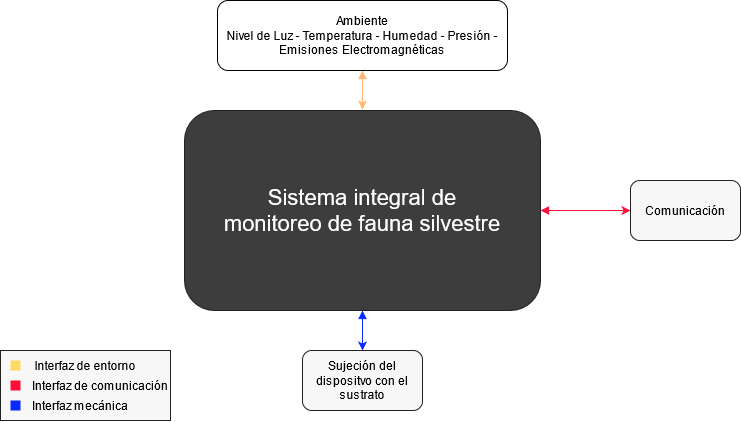
\includegraphics[width=\linewidth]{ImagenesDefinicion/func}
	\label{fig:diagrama_func_interfaces}
	\caption{Diagrama Funcional de Interfaces.}
\end{figure}

\subsection{Especificaciones de Diseño}
\subsubsection{Especificaciones Funcionales}
% Please add the following required packages to your document preamble:
% \usepackage{multirow}
\begin{table}[H]
\centering
\begin{tabular}{|c|c|}
\hline
\multicolumn{2}{|c|}{\textbf{Leyenda para especificaciones}}    \\ \hline
\textbf{Aplicabilidad}             & \textbf{Validación}        \\ \hline
\multirow{2}{*}{P: Prototipo}      & I: Inspección Visual       \\ \cline{2-2} 
                                   & D: Documentación de Diseño \\ \hline
\multirow{2}{*}{F: Producto Final} & S: Simulación              \\ \cline{2-2} 
                                   & T: Test                    \\ \hline
\end{tabular}
\end{table}
\note{Tabla Especificaciones Funcionales}

\note{Tabla 3.5: Especificaciones de Interfaz VOU}
\note{Tabla 3.6: Especificaciones de Interfaz MEC}
\note{Tabla 3.7: Especificaciones de Performance}
\note{Tabla 3.8: Especificaciones de Operación}
\note{Tabla 3.9: Especificaciones de Almacenamiento y Transporte}
\note{Tabla 3.11: Especificaciones Dimensionales y de Peso}
\note{Tabla 3.12: Especificaciones de costos}
\note{Tabla 3.13: Especificaciones de Confiabilidad}
\note{Tabla 3.14: Especificaciones de Disponibilidad}
\note{Tabla 3.15: Especificaciones de Mantenibilidad}
\note{Tabla 3.16: Especificaciones de Seguridad}


\end{document}

\Section{Plan de Validación}
%\documentclass[a4paper]{article}
%\usepackage[utf8]{inputenc}
\usepackage[spanish, es-tabla, es-noshorthands]{babel}
\usepackage[table,xcdraw,dvipsnames]{xcolor}
\usepackage[a4paper, footnotesep=1.25cm, headheight=1.25cm, top=2.54cm, left=2.54cm,
 bottom=2.54cm, right=2.54cm]{geometry}
%\geometry{showframe}
 \usepackage[normalem]{ulem}
 \useunder{\uline}{\ul}{}

%VERIFICAR EL HEAD Y EL FOOT EN
%https://ctan.dcc.uchile.cl/macros/latex/contrib/geometry/geometry.pdf

%Paquetes varios:
\usepackage{verbatimbox}

%\usepackage{wrapfig}			%Wrap figure in text
\usepackage[export]{adjustbox}	%Move images
\usepackage{changepage}			%Move tables
\usepackage{todonotes}

\usepackage{tikz}
\usepackage{amsmath}
\usepackage{amsfonts}
\usepackage{amssymb}
\usepackage{float}
\usepackage[graphicx]{realboxes}
\usepackage{caption}
\usepackage{subcaption}
\usepackage{multicol}
\usepackage{multirow}
\setlength{\doublerulesep}{\arrayrulewidth}
%\usepackage{booktabs}

\usepackage{array}
\newcolumntype{C}[1]{>{\centering\let\newline\\\arraybackslash\hspace{0pt}}m{#1}}
%\usepackage[american]{circuitikz}
\usetikzlibrary{calc}
\usepackage{fancyhdr}
\usepackage{units} 

\usepackage{colortbl}
%\usepackage{sectsty}
%\usepackage{unicode-math}

%FONTS (IMPORTANTE): Compilar en XeLaTex o LuaLaTeX
\usepackage{anyfontsize}	%Font size
\usepackage{fontspec}		%Font type
%Si sigue sin andar comentar \usepackage[utf8]{inputenc}
%https://ctan.dcc.uchile.cl/macros/unicodetex/latex/fontspec/fontspec.pdf
%https://www.overleaf.com/learn/latex/XeLaTeX

%Path para imagenes para trabajar en subarchivos
\graphicspath{{../Resumen/}{../Referencias/}{../Apendice/}{../Descripción de la Empresa/}{../Tareas del Alumno/}{../Conclusiones/}{../Herramientas Empleadas/}}

%Definiciones de nuevos comandos y colores
%COLORES:
\definecolor{AzulFoot}{rgb}{0.682,0.809,0.926}	%RGB	%{174,206,235}
\definecolor{AzulInfo}{rgb}{0.180,0.455,0.710}	%RGB	%{46,116,181}
\definecolor{AzulTable}{rgb}{0.302,0.507,0.871}	%RGB	%{68,114,196}
\definecolor{PName}{rgb}{0.353,0.353,0.353}		%RGB	%{90,90,90}
\definecolor{mygreen}{rgb}{28,172,0} % color values Red, Green, Blue
\definecolor{mylilas}{rgb}{170,55,241}

%Change Font Size

% #1 = size, #2 = text
\newcommand{\setparagraphsize}[2]{{\fontsize{#1}{6}\selectfont#2 \par}}		%Cambia el size de todo el parrafo
\newcommand{\setlinesize}[2]{{\fontsize{#1}{6}\selectfont#2}}				%Cambia el font de una oración

%IMAGE IN TABLE:			%Ejemplo: \includeintable{.3}{ImagenesFactibilidad/pend}
\renewcommand\fbox{\fcolorbox{white}{white}}
\setlength{\fboxrule}{0pt}	%padding thickness
\setlength{\fboxsep}{4pt}	%border thickness
\newcommand{\includeintable}[2]{	
	\fbox{
		\begin{minipage}{#1\textwidth}
        	\includegraphics[width=\linewidth]{#2}
    	\end{minipage}
	}
}

%LINK IN REF
\newcommand{\reflink}[1]{		%LINK
	\href{#1}{#1}
}

%NOTAS:
\newcommand{\note}[1]{		%RED BIG NOTE (TODO)
	\begin{center}
		\huge{ \textcolor{red}{#1} }
	\end{center}
}

\newcommand{\lnote}[1]{{\fontsize{14}{6}\selectfont\textcolor{green}{#1}}}	%Notas pequeñas

\newcommand{\observacion}[2]{  \ifnumequal{1}{#1}{ { \todo[inline,backgroundcolor=red!25,bordercolor=red!100]{\textbf{Observación: #2}} } }{  }  }

\newcommand{\red}[1]{\textcolor{red}{#1}}

\newcommand{\TBD}{\textcolor{red}{(TBD) }}
\newcommand{\tbd}{\textcolor{red}{(TBD) }}

\newcommand{\TBC}{\textcolor{red}{(TBC) }}
\newcommand{\tbc}{\textcolor{red}{(TBC) }}

\newcommand{\quotes}[1]{``#1''}
\newcommand{\q}[1]{``#1''}

\newcommand{\ip}{192.168.0.10:1880}
\newcommand{\ipadmin}{192.168.0.10:1880/admin}

% Comandos para agregar elementos en tablas de acronimos y definiciones
\newcommand{\addacronym}[2]{\textbf{#1} & \begin{tabular}[l]{@{}l@{}}#2\end{tabular} \\ \hline}

% tabItem
\newcommand{\tabitem}{~~\llap{\textbullet}~~}


\usepackage{hyperref}
\hypersetup{
    colorlinks=true,
    linkcolor=black,
    filecolor=magenta,      
    urlcolor=AzulInfo,
    citecolor=AzulInfo,    
}

%Configuración del header y del footer:
\usepackage{etoolbox}
\pagestyle{fancy}
\fancyhf{}
\rfoot{\thepage}
\renewcommand{\footrulewidth}{4pt}
\renewcommand{\headrulewidth}{0pt}
\patchcmd{\footrule}{\hrule}{\color{AzulFoot}\hrule}{}{}

%Código en el informe
%% IMPORTANTE:
% Verificar que esté \usepackage[dvipsnames]{xcolor}

%\usepackage{listingsutf8}
\usepackage{listings}

\renewcommand{\lstlistingname}{Código}

%LSTSET: Pone un recuadro y contador de linea en el codigo
\newcommand{\boxstyle}{
	\lstset{
		basicstyle=\sffamily\color{black},
		frame=single,
		numbers=left,
		numbersep=5pt,
		numberstyle=\color{gray},
		showspaces=false,
		showstringspaces=false
	}
}

\newcommand{\defaultstyle}{
	\lstset{
		basicstyle=\sffamily\color{white},
		frame=none,
		numbers=none,
		showspaces=true,
		showstringspaces=true
	}
}

\lstdefinelanguage{Kotlin}{
  captionpos=b,
  comment=[l]{//},
  commentstyle={\color{gray}\ttfamily},
  emph={filter, first, firstOrNull, forEach, lazy, map, mapNotNull, println},
  emphstyle={\color{OrangeRed}},
  identifierstyle=\color{black},
  keywords={!in, !is, abstract, actual, annotation, as, as?, break, by, catch, class, companion, const, constructor, continue, crossinline, data, delegate, do, dynamic, else, enum, expect, external, false, field, file, final, finally, for, fun, get, if, import, in, infix, init, inline, inner, interface, internal, is, lateinit, noinline, null, object, open, operator, out, override, package, param, private, property, protected, public, receiveris, reified, return, return@, sealed, set, setparam, super, suspend, tailrec, this, throw, true, try, typealias, typeof, val, var, vararg, when, where, while},
  keywordstyle={\color{NavyBlue}\bfseries},
  morecomment=[s]{/*}{*/},
  morestring=[b]",
  morestring=[s]{"""*}{*"""},
  ndkeywords={@Deprecated, @JvmField, @JvmName, @JvmOverloads, @JvmStatic, @JvmSynthetic, Array, Byte, Double, Float, Int, Integer, Iterable, Long, Runnable, Short, String, Any, Unit, Nothing},
  ndkeywordstyle={\color{BurntOrange}\bfseries},
  sensitive=true,
  stringstyle={\color{ForestGreen}\ttfamily},
}

\lstdefinelanguage{Swift}
{
  morekeywords={
    open,catch,@escaping,nil,throws,func,if,then,else,for,in,while,do,switch,case,default,where,break,continue,fallthrough,return,
    typealias,struct,class,enum,protocol,var,func,let,get,set,willSet,didSet,inout,init,deinit,extension,
    subscript,prefix,operator,infix,postfix,precedence,associativity,left,right,none,convenience,dynamic,
    final,lazy,mutating,nonmutating,optional,override,required,static,unowned,safe,weak,internal,
    private,public,is,as,self,unsafe,dynamicType,true,false,nil,Type,Protocol,
  },
  morecomment=[l]{//}, % l is for line comment
  morecomment=[s]{/*}{*/}, % s is for start and end delimiter
  morestring=[b]", % defines that strings are enclosed in double quotes
  breaklines=true,
  escapeinside={\%*}{*)},
  numbers=left,
  captionpos=b,
  breakatwhitespace=true,
  basicstyle=\linespread{1.0}\ttfamily, % https://tex.stackexchange.com/a/102728/129441
}

\definecolor{keyword}{HTML}{BA2CA3}
\definecolor{string}{HTML}{D12F1B}
\definecolor{comment}{HTML}{008400}

\newcommand{\swiftstyle}{
	\lstset{
  		language=Swift,
  		inputencoding=utf8x,
		extendedchars=\true,
	  	basicstyle=\ttfamily,
	  	showstringspaces=false, % lets spaces in strings appear as real spaces
  		columns=fixed,
  		keepspaces=true,
  		keywordstyle=\color{keyword},
  		stringstyle=\color{string},
  		commentstyle=\color{comment}
	}
}


%Como usarlo:

%\begin{lstlisting}[caption={Simple code listing.}, label={lst:example1}, language=Kotlin]
%// this is a simple code listing:
%println("hello kotlin from latex")
%\end{lstlisting}

%Si se corta en 2 páginas distintas:

%\vspace{1mm}
%\noindent{\begin{minipage}{\linewidth}
%\begin{lstlisting}[...]
%...
%\end{lstlisting}
%\end{minipage}}




\usepackage{titlesec}		%Para hacer las subsubsubsections

%Colores a los nombres de las secciones:
%\sectionfont{\color{AzulInfo}}  % sets color of sections
%\subsectionfont{\color{AzulInfo}}
%\subsubsectionfont{\color{AzulInfo}}

%PICTURES AND TABLE INDEX:
\newcommand{\Section}[1]{ \section{#1} 
	\phantomsection \setcounter{figure}{0} \setcounter{table}{0} \setcounter{lstlisting}{0}
		\renewcommand{\thetable}{\arabic{section}.\arabic{table}}
		\renewcommand{\thefigure}{\arabic{section}.\arabic{figure}}
		\renewcommand{\thelstlisting}{\arabic{section}.\arabic{lstlisting}}
}

\newcommand{\Subsection}[1]{ \subsection{#1}
	\phantomsection \setcounter{figure}{0} \setcounter{table}{0} \setcounter{lstlisting}{0}
		\renewcommand{\thetable}{\arabic{section}.\arabic{subsection}.\arabic{table}}
		\renewcommand{\thefigure}{\arabic{section}.\arabic{subsection}.\arabic{figure}}
		\renewcommand{\thelstlisting}{\arabic{section}.\arabic{subsection}.\arabic{lstlisting}}
}

\newcommand{\Subsubsection}[1]{ \subsubsection{#1} 
	\phantomsection \setcounter{figure}{0} \setcounter{table}{0}  \setcounter{lstlisting}{0}
		\renewcommand{\thetable}{\arabic{section}.\arabic{subsection}.\arabic{subsubsection}.\arabic{table}}
		\renewcommand{\thefigure}{\arabic{section}.\arabic{subsection}.\arabic{subsubsection}.\arabic{figure}}
		\renewcommand{\thelstlisting}{\arabic{section}.\arabic{subsection}.\arabic{subsubsection}.\arabic{lstlisting}}
}

%Definición de subsubsubsection:
\titleclass{\subsubsubsection}{straight}[\subsection]

\newcounter{subsubsubsection}[subsubsection]
\renewcommand\thesubsubsubsection{\thesubsubsection.\arabic{subsubsubsection}}

\titleformat{\subsubsubsection}
  {\normalfont\normalsize\bfseries\color{AzulInfo}}{\thesubsubsubsection}{1em}{}	%Color de subsubsubsection
\titlespacing*{\subsubsubsection}
{0pt}{3.25ex plus 1ex minus .2ex}{1.5ex plus .2ex}

\makeatletter
\renewcommand\paragraph{\@startsection{paragraph}{5}{\z@}%
  {3.25ex \@plus1ex \@minus.2ex}%
  {-1em}%
  {\normalfont\normalsize\bfseries}}
\renewcommand\subparagraph{\@startsection{subparagraph}{6}{\parindent}%
  {3.25ex \@plus1ex \@minus .2ex}%
  {-1em}%
  {\normalfont\normalsize\bfseries}}
\def\toclevel@subsubsubsection{4}
\def\toclevel@paragraph{5}
\def\toclevel@paragraph{6}
\def\l@subsubsubsection{\@dottedtocline{4}{7em}{4em}}
\def\l@paragraph{\@dottedtocline{5}{10em}{5em}}
\def\l@subparagraph{\@dottedtocline{6}{14em}{6em}}
\makeatother

\setcounter{secnumdepth}{4}
\setcounter{tocdepth}{4}

%Subsubsubsection:
\newcommand{\Subsubsubsection}[1]{ \subsubsubsection{#1} 
	\phantomsection \setcounter{figure}{0} \setcounter{table}{0} \renewcommand{\thetable}{\arabic{section}.\arabic{subsection}.\arabic{subsubsection}.\arabic{subsubsubsection}.\arabic{table}} \renewcommand{\thefigure}{\arabic{section}.\arabic{subsection}.\arabic{subsubsection}.\arabic{subsubsubsection}.\arabic{figure}}
}

%Tamaño, color e identación de sección, subsección, subsubsección y subsubsubsección:
%La identación de las subsecciones está tambien en Index-cfg.tex para el toc, lot y lot en el index
\titleformat{\section}[block]{\fontsize{16}{6}\selectfont\bfseries\color{AzulInfo}}{\thesection.}{1em}{} 
\titleformat{\subsection}[block]{\hspace{2.5em}\fontsize{13}{6}\selectfont\color{AzulInfo}}{\thesubsection}{1em}{}
\titleformat{\subsubsection}[block]{\hspace{3.5em}\fontsize{12}{6}\selectfont\color{AzulInfo}}{\thesubsubsection}{1em}{}
\titleformat{\subsubsubsection}[block]{\hspace{4em}\fontsize{11}{6}\selectfont\color{AzulInfo}}{\thesubsubsubsection}{1em}{}

%Pone las refrencias en el indice
\usepackage[numbib, nottoc, notlot, notlof]{tocbibind}

%Pone toc, lof y lot en colores y elijo el titulo de estos
\addto\captionsspanish{
	\renewcommand\contentsname{Contenidos}
	\renewcommand\listfigurename{Lista de Figuras}
	\renewcommand\listtablename{Lista de Tablas}
}

%Agrega TOC al indice
\renewcommand{\tableofcontents}{
	\stepcounter{section}
	\addcontentsline{toc}{section}{\protect\numberline{\thesection}\textbf{Contenidos}}
	\tableofcontents
}

%Agrega LOF al indice
\renewcommand{\listoffigures}{
	\stepcounter{section}
	\addcontentsline{toc}{section}{\protect\numberline{\thesection}\textbf{Lista de Figuras}}
	\listoffigures
}

%Agrega LOT al indice
\renewcommand{\listoftables}{
	\stepcounter{section}
	\addcontentsline{toc}{section}{\protect\numberline{\thesection}\textbf{Lista de Tablas}}
	\listoftables
}

%Indices: cambio la separación de los numeros para que entren tablas y fotos
\usepackage{tocloft}
\setlength{\cftfignumwidth}{1.35cm}  % change numwidth from figures in lof
\setlength{\cfttabnumwidth}{1.35cm}  % change numwidth from tables in lot
\renewcommand{\cfttoctitlefont}{\Large\bfseries\color{AzulInfo}}
\renewcommand{\cftloftitlefont}{\Large\bfseries\color{AzulInfo}}
\renewcommand{\cftlottitlefont}{\Large\bfseries\color{AzulInfo}}

%Coloca lineas punteadas a las seciones en el TOC
\renewcommand{\cftsecleader}{\cftdotfill{\cftdotsep}}

%Items con bullets y no cuadrados
\renewcommand{\labelitemi}{\textbullet }

%
%\begin{document}

\Subsection{Matriz de Trazabilidad de Validación}
\label{sec:MatrizTrazabilidad}
\begin{table}[H]
\centering
\begin{tabular}{|c|l|c|c|}
\hline
\multirow{2}{*}{\textbf{Origen}}               & \multicolumn{1}{c|}{\textbf{REQ ID}}                                                                                                                                                      & \multirow{2}{*}{\textbf{ESP ID}} & \multirow{2}{*}{\textbf{\begin{tabular}[c]{@{}c@{}}TEST ID o\\ sección\end{tabular}}} \\ \cline{2-2}
                                               & \multicolumn{1}{c|}{\textbf{Descripción corta}}                                                                                                                                           &                                  &                                                                                       \\ \hline
\multirow{6}{*}{Cliente}                       & REQ 01                                                                                                                                                                                    & INT-MEC-01                       &                                                                                       \\ \cline{2-2}
                                               & \multirow{5}{*}{\begin{tabular}[c]{@{}l@{}}El producto estará colgado de un árbol a (entre 4 m y 14 m)\\ y se instalará parcialmente dentro del nido del ave.\end{tabular}}               & INT-MEC-02                       & \TBC                                                                                  \\
                                               &                                                                                                                                                                                           & IMP-DIM-01                       & T-IMP-DIM-01                                                                          \\
                                               &                                                                                                                                                                                           & IMP-DIM-02                       & T-IMP-DIM-01                                                                          \\
                                               &                                                                                                                                                                                           & IMP-DIM-03                       & T-IMP-DIM-02                                                                          \\
                                               &                                                                                                                                                                                           & IMP-DIM-04                       & T-IMP-DIM-02                                                                          \\ \hline
\multirow{6}{*}{Cliente}                       & REQ 02                                                                                                                                                                                    & INT-FUN-02                       & T-INT-FUN-06                                                                          \\ \cline{2-2}
                                               & \multirow{5}{*}{\begin{tabular}[c]{@{}l@{}}El producto debe poder mantenerse energizado sin\\ intervención humana, minimizando pérdidas de\\ alimentación.\end{tabular}}                  & INT-FUN-03                       & T-INT-FUN-07                                                                          \\
                                               &                                                                                                                                                                                           & INT-FUN-04                       &                                                                                       \\
                                               &                                                                                                                                                                                           & PER-02                           & T-PER-01                                                                              \\
                                               &                                                                                                                                                                                           & PER-03                           & T-PER-02                                                                              \\
                                               &                                                                                                                                                                                           & PER-04                           & T-PER-03                                                                              \\ \hline
\multirow{3}{*}{Tácito}                        & REQ 03                                                                                                                                                                                    & INT-FUN-02                       & T-INT-FUN-06                                                                          \\ \cline{2-2}
                                               & \multirow{2}{*}{\begin{tabular}[c]{@{}l@{}}El producto no debe requerir conexión a la red eléctrica\\ para su funcionamiento\end{tabular}}                                                & INT-FUN-03                       & T-INT-FUN-07                                                                          \\
                                               &                                                                                                                                                                                           & INT-FUN-04                       &                                                                                       \\ \hline
\multirow{4}{*}{Cliente}                       & REQ 04                                                                                                                                                                                    & INT-FUN-01                       &                                                                                       \\ \cline{2-2}
                                               & \multirow{3}{*}{\begin{tabular}[c]{@{}l@{}}El producto debe ser capaz de adquirir los siguientes\\ datos dentro del nido:  temperatura, humedad, \TBD\end{tabular}}                       & INT-FUN-05                       & T-INT-FUN-01                                                                          \\
                                               &                                                                                                                                                                                           & INT-FUN-06                       & T-INT-FUN-08                                                                          \\
                                               &                                                                                                                                                                                           & INT-FUN-07                       & T-INT-FUN-02                                                                          \\ \hline
\multirow{5}{*}{Cliente}                       & REQ 05                                                                                                                                                                                    & INT-FUN-09                       & T-INT-COM1-05                                                                         \\ \cline{2-2}
                                               & \multirow{4}{*}{\begin{tabular}[c]{@{}l@{}}Un dispositivo ajeno al proyecto que irá sobre el ave\\ debe poder transmitirle los datos que adquirió\\ durante el día al nido.\end{tabular}} & INT-COM1-01                      & T-INT-COM1-01                                                                         \\
                                               &                                                                                                                                                                                           & INT-COM1-02                      & T-INT-COM1-02                                                                         \\
                                               &                                                                                                                                                                                           & INT-COM1-03                      & T-INT-COM1-03                                                                         \\
                                               &                                                                                                                                                                                           & INT-COM1-04                      & T-INT-COM1-04                                                                         \\ \hline
\multirow{2}{*}{Tácito}                        & REQ 06                                                                                                                                                                                    & INT-FUN-01                       &                                                                                       \\ \cline{2-2}
                                               & \begin{tabular}[c]{@{}l@{}}El producto debe poder almacenar los datos adquiridos\\ por el nido y el ave.\end{tabular}                                                                     &                                  &                                                                                       \\ \hline
\multirow{8}{*}{Cliente}                       & REQ 07                                                                                                                                                                                    & INT-FUN-08                       & T-INT-COM2-07                                                                         \\ \cline{2-2}
                                               & \multirow{7}{*}{\begin{tabular}[c]{@{}l@{}}Una persona debe poder recibir los datos almacenados\\ en el nido a la distancia.\end{tabular}}                                                & INT-COM2-01                      & T-INT-COM2-01                                                                         \\
                                               &                                                                                                                                                                                           & INT-COM2-03                      & T-INT-COM2-03                                                                         \\
                                               &                                                                                                                                                                                           & INT-COM2-04                      & T-INT-COM2-04                                                                         \\
                                               &                                                                                                                                                                                           & INT-COM2-05                      & T-INT-COM2-05                                                                         \\
                                               &                                                                                                                                                                                           & INT-COM2-06                      & T-INT-COM2-06                                                                         \\
                                               &                                                                                                                                                                                           & PER-04                           & T-PER-03                                                                              \\
                                               &                                                                                                                                                                                           & RAM-SEG-03                       & T-RAM-SEG-01                                                                          \\ \hline
\multicolumn{1}{|l|}{\multirow{2}{*}{Cliente}} & REQ 08                                                                                                                                                                                    & \multicolumn{1}{l|}{INT-AMB-01}  & \multicolumn{1}{l|}{}                                                                 \\ \cline{2-2}
\multicolumn{1}{|l|}{}                         & \begin{tabular}[c]{@{}l@{}}El producto no debe llamar la atención de humanos\\ desde el nivel del piso\end{tabular}                                                                       & \multicolumn{1}{l|}{INT-AMB-02}  & \multicolumn{1}{l|}{}                                                                 \\ \hline
\end{tabular}
\caption{Matriz de trazabilidad (Parte 1).}
\end{table}

\begin{table}[H]
\centering
\begin{tabular}{|c|l|c|c|}
\hline
\multirow{2}{*}{\textbf{Origen}} & \multicolumn{1}{c|}{\textbf{REQ ID}}                                                                                                                                                                                 & \multirow{2}{*}{\textbf{ESP ID}} & \multirow{2}{*}{\textbf{\begin{tabular}[c]{@{}c@{}}TEST ID o\\ sección\end{tabular}}} \\ \cline{2-2}
                                 & \multicolumn{1}{c|}{\textbf{Descripción corta}}                                                                                                                                                                      &                                  &                                                                                       \\ \hline
\multirow{3}{*}{Tácito}          & REQ 09                                                                                                                                                                                                               & IMP-DIM-02                       & T-IMP-DIM-01                                                                          \\ \cline{2-2}
                                 & \multirow{2}{*}{\begin{tabular}[c]{@{}l@{}}El producto o su instalación no debe dañar\\ significativamente al árbol donde estará el nido.\end{tabular}}                                                              & IMP-DIM-03                       & T-IMP-DIM-02                                                                          \\
                                 &                                                                                                                                                                                                                      & IMP-DIM-04                       & T-IMP-DIM-02                                                                          \\ \hline
\multirow{10}{*}{Tácito}         & REQ 10                                                                                                                                                                                                               & IMP-AYT-01                       &                                                                                       \\ \cline{2-2}
                                 & \multirow{9}{*}{\begin{tabular}[c]{@{}l@{}}El producto debe soportar las condiciones meteorológicas\\ del sur Argentino, específicamente los alrededores de\\ Bariloche, Rio Negro.\end{tabular}}                    & IMP-AYT-02                       &                                                                                       \\
                                 &                                                                                                                                                                                                                      & IMP-AYT-03                       &                                                                                       \\
                                 &                                                                                                                                                                                                                      & IMP-AYT-04                       &                                                                                       \\
                                 &                                                                                                                                                                                                                      & IMP-OPE-01                       &                                                                                       \\
                                 &                                                                                                                                                                                                                      & IMP-OPE-02                       &                                                                                       \\
                                 &                                                                                                                                                                                                                      & IMP-OPE-03                       &                                                                                       \\
                                 &                                                                                                                                                                                                                      & IMP-OPE-04                       &                                                                                       \\
                                 &                                                                                                                                                                                                                      & INT-MEC-01                       &                                                                                       \\
                                 &                                                                                                                                                                                                                      & INT-MEC-02                       & \TBC                                                                                  \\ \hline
\multirow{2}{*}{Cliente}         & REQ 11                                                                                                                                                                                                               & IMP-COS-01                       &                                                                                       \\ \cline{2-2}
                                 & El producto debe costar menos de \TBD USD.                                                                                                                                                                           & IMP-COS-02                       &                                                                                       \\ \hline
\multirow{2}{*}{Estado}          & REQ 12                                                                                                                                                                                                               & RAM-SEG-01                       & \TBC                                                                                  \\ \cline{2-2}
                                 & \begin{tabular}[c]{@{}l@{}}El producto debe cumplir la norma \TBD: seguridad\\ eléctrica.\end{tabular}                                                                                                               & RAM-SEG-05                       &                                                                                       \\ \hline
\multirow{2}{*}{Estado}          & REQ 13                                                                                                                                                                                                               & IMP-EMC-01                       &                                                                                       \\ \cline{2-2}
                                 & \begin{tabular}[c]{@{}l@{}}El producto debe cumplir la norma \TBD: compatibilidad\\ electromagnética.\end{tabular}                                                                                                   &                                  &                                                                                       \\ \hline
\multirow{2}{*}{Estado}          & REQ 14                                                                                                                                                                                                               & RAM-SEG-04                       &                                                                                       \\ \cline{2-2}
                                 & \begin{tabular}[c]{@{}l@{}}El producto debe cumplir la norma \TBD: seguridad\\ ambiental.\end{tabular}                                                                                                               & INT-AMB-04                       &                                                                                       \\ \hline
\multirow{3}{*}{Cliente}         & REQ 15                                                                                                                                                                                                               & PER-01                           & T-PER-04                                                                              \\ \cline{2-2}
                                 & \multirow{2}{*}{\begin{tabular}[c]{@{}l@{}}El producto debe poder cargar las baterias del\\ dispositivo del ave.\end{tabular}}                                                                                       & PER-03                           & T-PER-02                                                                              \\
                                 &                                                                                                                                                                                                                      & INT-FUN-10                       & T-INT-FUN-09                                                                          \\ \hline
\multirow{7}{*}{Cliente}         & REQ 16                                                                                                                                                                                                               & INT-AMB-01                       &                                                                                       \\ \cline{2-2}
                                 & \multirow{6}{*}{\begin{tabular}[c]{@{}l@{}}El producto debe perturbar lo mínimo posible a las\\ aves dentro del nido o cambiar lo menos posible, su\\ comportamiento, el cual es el objeto de estudio.\end{tabular}} & INT-AMB-02                       &                                                                                       \\
                                 &                                                                                                                                                                                                                      & INT-AMB-03                       &                                                                                       \\
                                 &                                                                                                                                                                                                                      & INT-COM1-01                      & T-INT-COM1-01                                                                         \\
                                 &                                                                                                                                                                                                                      & INT-COM1-03                      & T-INT-COM1-03                                                                         \\
                                 &                                                                                                                                                                                                                      & INT-COM2-02                      & T-INT-COM1-02                                                                         \\
                                 &                                                                                                                                                                                                                      & RAM-SEG-01                       & \TBC                                                                                  \\ \hline
\multirow{4}{*}{Tácito}          & REQ 17                                                                                                                                                                                                               & IMP-AYT-01                       &                                                                                       \\ \cline{2-2}
                                 & \multirow{3}{*}{\begin{tabular}[c]{@{}l@{}}El producto desarmado debe soportar las condiciones\\ de translado impuestas por los caminos rurales hasta\\ llegar a la zona de instalación.\end{tabular}}               & IMP-AYT-02                       &                                                                                       \\
                                 &                                                                                                                                                                                                                      & IMP-AYT-03                       &                                                                                       \\
                                 &                                                                                                                                                                                                                      & IMP-AYT-04                       &                                                                                       \\ \hline
\multirow{2}{*}{Tácito}          & REQ 18                                                                                                                                                                                                               & INT-FUN-12                       & T-INT-FUN-04                                                                          \\ \cline{2-2}
                                 & \begin{tabular}[c]{@{}l@{}}La tasa de adquisición de datos debe ser sensata y\\ dependerá de cada variable a medir.\end{tabular}                                                                                      &                                  &                                                                                       \\ \hline
\multirow{2}{*}{Cliente}         & REQ 19                                                                                                                                                                                                               & RAM-CON-01                       &                                                                                       \\ \cline{2-2}
                                 & \begin{tabular}[c]{@{}l@{}}La vida útil del producto deberá ser de por lo menos\\ 2 años.\end{tabular}                                                                                                               &                                  &                                                                                       \\ \hline
\end{tabular}
\caption{Matriz de trazabilidad (Parte 2).}
\end{table}

\Subsection{Plan de Verificación y Validación }
\label{sec:PlanValidacion}
\begin{table}[H]
\centering
\begin{tabular}{|l|c|}
\hline
\multicolumn{1}{|c|}{Aspecto}             & ID del test   \\ \hline
Adquisicion de datos de temperatura       & T-INT-FUN-01  \\ \hline
Adquisicion de datos de luminosidad       & T-INT-FUN-02  \\ \hline
Adquisicion de datos de humedad           & T-INT-FUN-03  \\ \hline
Adquisicion de imágenes                   & T-INT-FUN-04  \\ \hline
Adquisicion de video                      & T-INT-FUN-05  \\ \hline
Periodo activación sensor temperatura     & T-INT-FUN-06  \\ \hline
Periodo activación sensor luminosidad     & T-INT-FUN-07  \\ \hline
Periodo activación sensor humedad         & T-INT-FUN-08  \\ \hline
Periodo activación de la cámara           & T-INT-FUN-09  \\ \hline
Recuperación ante pérdida de alimentación & T-INT-FUN-10  \\ \hline
Adquisición de datos de presencia         & T-INT-FUN-11  \\ \hline
Recolección de energía en condiciones similares a las de instalación                                     & T-INT-FUN-12 \\ \hline
Transmisión de video en tiempo real de dentro del nido                                                   & T-INT-FUN-13 \\ \hline
Periodo detección de la presencia         & T-INT-FUN-14  \\ \hline
Validación del almacenamiento de datos    & T-INT-FUN-15  \\ \hline
Validación de fecha y hora cierta         & T-INT-FUN-16  \\ \hline
\begin{tabular}[c]{@{}l@{}}Validación de fecha y hora cierta tras\\ pérdida de alimentación\end{tabular} & T-INT-FUN-17 \\ \hline
Consistencia de datos COM1                & T-INT-COM1-01 \\ \hline
Alcance transmisión COM1                  & T-INT-COM1-02 \\ \hline
Consistencia de datos COM2                & T-INT-COM2-01 \\ \hline
Alcance transmisión COM2                  & T-INT-COM2-02 \\ \hline
Descarte de datos COM2                    & T-INT-COM2-03 \\ \hline
Validación dimensiones totales            & T-IMP-DIM-01  \\ \hline
Validación peso total                     & T-IMP-DIM-02  \\ \hline
Autorización transmisión nido-persona     & T-RAM-SEG-01  \\ \hline
\end{tabular}
\caption{Tabla de plan de validación}
\end{table}

%\end{document}

\Section{Análisis de Factibilidad}
\documentclass[a4paper]{article}
%\usepackage[utf8]{inputenc}
\usepackage[spanish, es-tabla, es-noshorthands]{babel}
\usepackage[table,xcdraw,dvipsnames]{xcolor}
\usepackage[a4paper, footnotesep=1.25cm, headheight=1.25cm, top=2.54cm, left=2.54cm,
 bottom=2.54cm, right=2.54cm]{geometry}
%\geometry{showframe}
 \usepackage[normalem]{ulem}
 \useunder{\uline}{\ul}{}

%VERIFICAR EL HEAD Y EL FOOT EN
%https://ctan.dcc.uchile.cl/macros/latex/contrib/geometry/geometry.pdf

%Paquetes varios:
\usepackage{verbatimbox}

%\usepackage{wrapfig}			%Wrap figure in text
\usepackage[export]{adjustbox}	%Move images
\usepackage{changepage}			%Move tables
\usepackage{todonotes}

\usepackage{tikz}
\usepackage{amsmath}
\usepackage{amsfonts}
\usepackage{amssymb}
\usepackage{float}
\usepackage[graphicx]{realboxes}
\usepackage{caption}
\usepackage{subcaption}
\usepackage{multicol}
\usepackage{multirow}
\setlength{\doublerulesep}{\arrayrulewidth}
%\usepackage{booktabs}

\usepackage{array}
\newcolumntype{C}[1]{>{\centering\let\newline\\\arraybackslash\hspace{0pt}}m{#1}}
%\usepackage[american]{circuitikz}
\usetikzlibrary{calc}
\usepackage{fancyhdr}
\usepackage{units} 

\usepackage{colortbl}
%\usepackage{sectsty}
%\usepackage{unicode-math}

%FONTS (IMPORTANTE): Compilar en XeLaTex o LuaLaTeX
\usepackage{anyfontsize}	%Font size
\usepackage{fontspec}		%Font type
%Si sigue sin andar comentar \usepackage[utf8]{inputenc}
%https://ctan.dcc.uchile.cl/macros/unicodetex/latex/fontspec/fontspec.pdf
%https://www.overleaf.com/learn/latex/XeLaTeX

%Path para imagenes para trabajar en subarchivos
\graphicspath{{../Resumen/}{../Referencias/}{../Apendice/}{../Descripción de la Empresa/}{../Tareas del Alumno/}{../Conclusiones/}{../Herramientas Empleadas/}}

%Definiciones de nuevos comandos y colores
%COLORES:
\definecolor{AzulFoot}{rgb}{0.682,0.809,0.926}	%RGB	%{174,206,235}
\definecolor{AzulInfo}{rgb}{0.180,0.455,0.710}	%RGB	%{46,116,181}
\definecolor{AzulTable}{rgb}{0.302,0.507,0.871}	%RGB	%{68,114,196}
\definecolor{PName}{rgb}{0.353,0.353,0.353}		%RGB	%{90,90,90}
\definecolor{mygreen}{rgb}{28,172,0} % color values Red, Green, Blue
\definecolor{mylilas}{rgb}{170,55,241}

%Change Font Size

% #1 = size, #2 = text
\newcommand{\setparagraphsize}[2]{{\fontsize{#1}{6}\selectfont#2 \par}}		%Cambia el size de todo el parrafo
\newcommand{\setlinesize}[2]{{\fontsize{#1}{6}\selectfont#2}}				%Cambia el font de una oración

%IMAGE IN TABLE:			%Ejemplo: \includeintable{.3}{ImagenesFactibilidad/pend}
\renewcommand\fbox{\fcolorbox{white}{white}}
\setlength{\fboxrule}{0pt}	%padding thickness
\setlength{\fboxsep}{4pt}	%border thickness
\newcommand{\includeintable}[2]{	
	\fbox{
		\begin{minipage}{#1\textwidth}
        	\includegraphics[width=\linewidth]{#2}
    	\end{minipage}
	}
}

%LINK IN REF
\newcommand{\reflink}[1]{		%LINK
	\href{#1}{#1}
}

%NOTAS:
\newcommand{\note}[1]{		%RED BIG NOTE (TODO)
	\begin{center}
		\huge{ \textcolor{red}{#1} }
	\end{center}
}

\newcommand{\lnote}[1]{{\fontsize{14}{6}\selectfont\textcolor{green}{#1}}}	%Notas pequeñas

\newcommand{\observacion}[2]{  \ifnumequal{1}{#1}{ { \todo[inline,backgroundcolor=red!25,bordercolor=red!100]{\textbf{Observación: #2}} } }{  }  }

\newcommand{\red}[1]{\textcolor{red}{#1}}

\newcommand{\TBD}{\textcolor{red}{(TBD) }}
\newcommand{\tbd}{\textcolor{red}{(TBD) }}

\newcommand{\TBC}{\textcolor{red}{(TBC) }}
\newcommand{\tbc}{\textcolor{red}{(TBC) }}

\newcommand{\quotes}[1]{``#1''}
\newcommand{\q}[1]{``#1''}

\newcommand{\ip}{192.168.0.10:1880}
\newcommand{\ipadmin}{192.168.0.10:1880/admin}

% Comandos para agregar elementos en tablas de acronimos y definiciones
\newcommand{\addacronym}[2]{\textbf{#1} & \begin{tabular}[l]{@{}l@{}}#2\end{tabular} \\ \hline}

% tabItem
\newcommand{\tabitem}{~~\llap{\textbullet}~~}


\usepackage{hyperref}
\hypersetup{
    colorlinks=true,
    linkcolor=black,
    filecolor=magenta,      
    urlcolor=AzulInfo,
    citecolor=AzulInfo,    
}

%Configuración del header y del footer:
\usepackage{etoolbox}
\pagestyle{fancy}
\fancyhf{}
\rfoot{\thepage}
\renewcommand{\footrulewidth}{4pt}
\renewcommand{\headrulewidth}{0pt}
\patchcmd{\footrule}{\hrule}{\color{AzulFoot}\hrule}{}{}

%Código en el informe
%% IMPORTANTE:
% Verificar que esté \usepackage[dvipsnames]{xcolor}

%\usepackage{listingsutf8}
\usepackage{listings}

\renewcommand{\lstlistingname}{Código}

%LSTSET: Pone un recuadro y contador de linea en el codigo
\newcommand{\boxstyle}{
	\lstset{
		basicstyle=\sffamily\color{black},
		frame=single,
		numbers=left,
		numbersep=5pt,
		numberstyle=\color{gray},
		showspaces=false,
		showstringspaces=false
	}
}

\newcommand{\defaultstyle}{
	\lstset{
		basicstyle=\sffamily\color{white},
		frame=none,
		numbers=none,
		showspaces=true,
		showstringspaces=true
	}
}

\lstdefinelanguage{Kotlin}{
  captionpos=b,
  comment=[l]{//},
  commentstyle={\color{gray}\ttfamily},
  emph={filter, first, firstOrNull, forEach, lazy, map, mapNotNull, println},
  emphstyle={\color{OrangeRed}},
  identifierstyle=\color{black},
  keywords={!in, !is, abstract, actual, annotation, as, as?, break, by, catch, class, companion, const, constructor, continue, crossinline, data, delegate, do, dynamic, else, enum, expect, external, false, field, file, final, finally, for, fun, get, if, import, in, infix, init, inline, inner, interface, internal, is, lateinit, noinline, null, object, open, operator, out, override, package, param, private, property, protected, public, receiveris, reified, return, return@, sealed, set, setparam, super, suspend, tailrec, this, throw, true, try, typealias, typeof, val, var, vararg, when, where, while},
  keywordstyle={\color{NavyBlue}\bfseries},
  morecomment=[s]{/*}{*/},
  morestring=[b]",
  morestring=[s]{"""*}{*"""},
  ndkeywords={@Deprecated, @JvmField, @JvmName, @JvmOverloads, @JvmStatic, @JvmSynthetic, Array, Byte, Double, Float, Int, Integer, Iterable, Long, Runnable, Short, String, Any, Unit, Nothing},
  ndkeywordstyle={\color{BurntOrange}\bfseries},
  sensitive=true,
  stringstyle={\color{ForestGreen}\ttfamily},
}

\lstdefinelanguage{Swift}
{
  morekeywords={
    open,catch,@escaping,nil,throws,func,if,then,else,for,in,while,do,switch,case,default,where,break,continue,fallthrough,return,
    typealias,struct,class,enum,protocol,var,func,let,get,set,willSet,didSet,inout,init,deinit,extension,
    subscript,prefix,operator,infix,postfix,precedence,associativity,left,right,none,convenience,dynamic,
    final,lazy,mutating,nonmutating,optional,override,required,static,unowned,safe,weak,internal,
    private,public,is,as,self,unsafe,dynamicType,true,false,nil,Type,Protocol,
  },
  morecomment=[l]{//}, % l is for line comment
  morecomment=[s]{/*}{*/}, % s is for start and end delimiter
  morestring=[b]", % defines that strings are enclosed in double quotes
  breaklines=true,
  escapeinside={\%*}{*)},
  numbers=left,
  captionpos=b,
  breakatwhitespace=true,
  basicstyle=\linespread{1.0}\ttfamily, % https://tex.stackexchange.com/a/102728/129441
}

\definecolor{keyword}{HTML}{BA2CA3}
\definecolor{string}{HTML}{D12F1B}
\definecolor{comment}{HTML}{008400}

\newcommand{\swiftstyle}{
	\lstset{
  		language=Swift,
  		inputencoding=utf8x,
		extendedchars=\true,
	  	basicstyle=\ttfamily,
	  	showstringspaces=false, % lets spaces in strings appear as real spaces
  		columns=fixed,
  		keepspaces=true,
  		keywordstyle=\color{keyword},
  		stringstyle=\color{string},
  		commentstyle=\color{comment}
	}
}


%Como usarlo:

%\begin{lstlisting}[caption={Simple code listing.}, label={lst:example1}, language=Kotlin]
%// this is a simple code listing:
%println("hello kotlin from latex")
%\end{lstlisting}

%Si se corta en 2 páginas distintas:

%\vspace{1mm}
%\noindent{\begin{minipage}{\linewidth}
%\begin{lstlisting}[...]
%...
%\end{lstlisting}
%\end{minipage}}




\usepackage{titlesec}		%Para hacer las subsubsubsections

%Colores a los nombres de las secciones:
%\sectionfont{\color{AzulInfo}}  % sets color of sections
%\subsectionfont{\color{AzulInfo}}
%\subsubsectionfont{\color{AzulInfo}}

%PICTURES AND TABLE INDEX:
\newcommand{\Section}[1]{ \section{#1} 
	\phantomsection \setcounter{figure}{0} \setcounter{table}{0} \setcounter{lstlisting}{0}
		\renewcommand{\thetable}{\arabic{section}.\arabic{table}}
		\renewcommand{\thefigure}{\arabic{section}.\arabic{figure}}
		\renewcommand{\thelstlisting}{\arabic{section}.\arabic{lstlisting}}
}

\newcommand{\Subsection}[1]{ \subsection{#1}
	\phantomsection \setcounter{figure}{0} \setcounter{table}{0} \setcounter{lstlisting}{0}
		\renewcommand{\thetable}{\arabic{section}.\arabic{subsection}.\arabic{table}}
		\renewcommand{\thefigure}{\arabic{section}.\arabic{subsection}.\arabic{figure}}
		\renewcommand{\thelstlisting}{\arabic{section}.\arabic{subsection}.\arabic{lstlisting}}
}

\newcommand{\Subsubsection}[1]{ \subsubsection{#1} 
	\phantomsection \setcounter{figure}{0} \setcounter{table}{0}  \setcounter{lstlisting}{0}
		\renewcommand{\thetable}{\arabic{section}.\arabic{subsection}.\arabic{subsubsection}.\arabic{table}}
		\renewcommand{\thefigure}{\arabic{section}.\arabic{subsection}.\arabic{subsubsection}.\arabic{figure}}
		\renewcommand{\thelstlisting}{\arabic{section}.\arabic{subsection}.\arabic{subsubsection}.\arabic{lstlisting}}
}

%Definición de subsubsubsection:
\titleclass{\subsubsubsection}{straight}[\subsection]

\newcounter{subsubsubsection}[subsubsection]
\renewcommand\thesubsubsubsection{\thesubsubsection.\arabic{subsubsubsection}}

\titleformat{\subsubsubsection}
  {\normalfont\normalsize\bfseries\color{AzulInfo}}{\thesubsubsubsection}{1em}{}	%Color de subsubsubsection
\titlespacing*{\subsubsubsection}
{0pt}{3.25ex plus 1ex minus .2ex}{1.5ex plus .2ex}

\makeatletter
\renewcommand\paragraph{\@startsection{paragraph}{5}{\z@}%
  {3.25ex \@plus1ex \@minus.2ex}%
  {-1em}%
  {\normalfont\normalsize\bfseries}}
\renewcommand\subparagraph{\@startsection{subparagraph}{6}{\parindent}%
  {3.25ex \@plus1ex \@minus .2ex}%
  {-1em}%
  {\normalfont\normalsize\bfseries}}
\def\toclevel@subsubsubsection{4}
\def\toclevel@paragraph{5}
\def\toclevel@paragraph{6}
\def\l@subsubsubsection{\@dottedtocline{4}{7em}{4em}}
\def\l@paragraph{\@dottedtocline{5}{10em}{5em}}
\def\l@subparagraph{\@dottedtocline{6}{14em}{6em}}
\makeatother

\setcounter{secnumdepth}{4}
\setcounter{tocdepth}{4}

%Subsubsubsection:
\newcommand{\Subsubsubsection}[1]{ \subsubsubsection{#1} 
	\phantomsection \setcounter{figure}{0} \setcounter{table}{0} \renewcommand{\thetable}{\arabic{section}.\arabic{subsection}.\arabic{subsubsection}.\arabic{subsubsubsection}.\arabic{table}} \renewcommand{\thefigure}{\arabic{section}.\arabic{subsection}.\arabic{subsubsection}.\arabic{subsubsubsection}.\arabic{figure}}
}

%Tamaño, color e identación de sección, subsección, subsubsección y subsubsubsección:
%La identación de las subsecciones está tambien en Index-cfg.tex para el toc, lot y lot en el index
\titleformat{\section}[block]{\fontsize{16}{6}\selectfont\bfseries\color{AzulInfo}}{\thesection.}{1em}{} 
\titleformat{\subsection}[block]{\hspace{2.5em}\fontsize{13}{6}\selectfont\color{AzulInfo}}{\thesubsection}{1em}{}
\titleformat{\subsubsection}[block]{\hspace{3.5em}\fontsize{12}{6}\selectfont\color{AzulInfo}}{\thesubsubsection}{1em}{}
\titleformat{\subsubsubsection}[block]{\hspace{4em}\fontsize{11}{6}\selectfont\color{AzulInfo}}{\thesubsubsubsection}{1em}{}

%Pone las refrencias en el indice
\usepackage[numbib, nottoc, notlot, notlof]{tocbibind}

%Pone toc, lof y lot en colores y elijo el titulo de estos
\addto\captionsspanish{
	\renewcommand\contentsname{Contenidos}
	\renewcommand\listfigurename{Lista de Figuras}
	\renewcommand\listtablename{Lista de Tablas}
}

%Agrega TOC al indice
\renewcommand{\tableofcontents}{
	\stepcounter{section}
	\addcontentsline{toc}{section}{\protect\numberline{\thesection}\textbf{Contenidos}}
	\tableofcontents
}

%Agrega LOF al indice
\renewcommand{\listoffigures}{
	\stepcounter{section}
	\addcontentsline{toc}{section}{\protect\numberline{\thesection}\textbf{Lista de Figuras}}
	\listoffigures
}

%Agrega LOT al indice
\renewcommand{\listoftables}{
	\stepcounter{section}
	\addcontentsline{toc}{section}{\protect\numberline{\thesection}\textbf{Lista de Tablas}}
	\listoftables
}

%Indices: cambio la separación de los numeros para que entren tablas y fotos
\usepackage{tocloft}
\setlength{\cftfignumwidth}{1.35cm}  % change numwidth from figures in lof
\setlength{\cfttabnumwidth}{1.35cm}  % change numwidth from tables in lot
\renewcommand{\cfttoctitlefont}{\Large\bfseries\color{AzulInfo}}
\renewcommand{\cftloftitlefont}{\Large\bfseries\color{AzulInfo}}
\renewcommand{\cftlottitlefont}{\Large\bfseries\color{AzulInfo}}

%Coloca lineas punteadas a las seciones en el TOC
\renewcommand{\cftsecleader}{\cftdotfill{\cftdotsep}}

%Items con bullets y no cuadrados
\renewcommand{\labelitemi}{\textbullet }


\begin{document}

\Subsection{Factibilidad tecnológica}
\Subsubsection{Esquema modular}
\Subsubsection{Propuesta de alternativas de diseño}
Para la medición de la temperatura se tuvieron en cuenta las diversas tecnologías que existen, poniendo en la balanza parametros que definen su performance tales como la linealidad de su salida, el costo, el rango de operación, la presición, tipo de salida y aplicación.
También se valoraron las diversas tecnologías que existen tales como la RTD cuyo funcionamiento se basa en el cambio de la resistencia en función de la temperatura bajo al ecuación $R(T)=R_0 + \alpha \cdot \Delta T$ también se consideró la tecnología TC la cual se basa en el \textit{efecto seebek} y finalmente el uso de un IC el cual es basado en propiedades de dispositivos semiconductores extrínsecos.
\Subsubsection{Elección de una solución}
\Subsubsection{DFMEA}

\Subsection{Factibilidad de tiempos}

\Subsubsection{Planificación}
(PERT y simulación de Montecarlo)

\Subsubsection{Programación}
(Gantt)

\Subsection{Factibilidad económica}
(Mercado, costos, ciclo de vida, VAN, TIR)

\Subsection{Factibilidad legal y responsabilidad civil}
(regulaciones y licencias)

\end{document}


\Section{Ingeniería de Detalle}
%\documentclass[a4paper]{article}
%\usepackage[utf8]{inputenc}
\usepackage[spanish, es-tabla, es-noshorthands]{babel}
\usepackage[table,xcdraw,dvipsnames]{xcolor}
\usepackage[a4paper, footnotesep=1.25cm, headheight=1.25cm, top=2.54cm, left=2.54cm,
 bottom=2.54cm, right=2.54cm]{geometry}
%\geometry{showframe}
 \usepackage[normalem]{ulem}
 \useunder{\uline}{\ul}{}

%VERIFICAR EL HEAD Y EL FOOT EN
%https://ctan.dcc.uchile.cl/macros/latex/contrib/geometry/geometry.pdf

%Paquetes varios:
\usepackage{verbatimbox}

%\usepackage{wrapfig}			%Wrap figure in text
\usepackage[export]{adjustbox}	%Move images
\usepackage{changepage}			%Move tables
\usepackage{todonotes}

\usepackage{tikz}
\usepackage{amsmath}
\usepackage{amsfonts}
\usepackage{amssymb}
\usepackage{float}
\usepackage[graphicx]{realboxes}
\usepackage{caption}
\usepackage{subcaption}
\usepackage{multicol}
\usepackage{multirow}
\setlength{\doublerulesep}{\arrayrulewidth}
%\usepackage{booktabs}

\usepackage{array}
\newcolumntype{C}[1]{>{\centering\let\newline\\\arraybackslash\hspace{0pt}}m{#1}}
%\usepackage[american]{circuitikz}
\usetikzlibrary{calc}
\usepackage{fancyhdr}
\usepackage{units} 

\usepackage{colortbl}
%\usepackage{sectsty}
%\usepackage{unicode-math}

%FONTS (IMPORTANTE): Compilar en XeLaTex o LuaLaTeX
\usepackage{anyfontsize}	%Font size
\usepackage{fontspec}		%Font type
%Si sigue sin andar comentar \usepackage[utf8]{inputenc}
%https://ctan.dcc.uchile.cl/macros/unicodetex/latex/fontspec/fontspec.pdf
%https://www.overleaf.com/learn/latex/XeLaTeX

%Path para imagenes para trabajar en subarchivos
\graphicspath{{../Resumen/}{../Referencias/}{../Apendice/}{../Descripción de la Empresa/}{../Tareas del Alumno/}{../Conclusiones/}{../Herramientas Empleadas/}}

%Definiciones de nuevos comandos y colores
%COLORES:
\definecolor{AzulFoot}{rgb}{0.682,0.809,0.926}	%RGB	%{174,206,235}
\definecolor{AzulInfo}{rgb}{0.180,0.455,0.710}	%RGB	%{46,116,181}
\definecolor{AzulTable}{rgb}{0.302,0.507,0.871}	%RGB	%{68,114,196}
\definecolor{PName}{rgb}{0.353,0.353,0.353}		%RGB	%{90,90,90}
\definecolor{mygreen}{rgb}{28,172,0} % color values Red, Green, Blue
\definecolor{mylilas}{rgb}{170,55,241}

%Change Font Size

% #1 = size, #2 = text
\newcommand{\setparagraphsize}[2]{{\fontsize{#1}{6}\selectfont#2 \par}}		%Cambia el size de todo el parrafo
\newcommand{\setlinesize}[2]{{\fontsize{#1}{6}\selectfont#2}}				%Cambia el font de una oración

%IMAGE IN TABLE:			%Ejemplo: \includeintable{.3}{ImagenesFactibilidad/pend}
\renewcommand\fbox{\fcolorbox{white}{white}}
\setlength{\fboxrule}{0pt}	%padding thickness
\setlength{\fboxsep}{4pt}	%border thickness
\newcommand{\includeintable}[2]{	
	\fbox{
		\begin{minipage}{#1\textwidth}
        	\includegraphics[width=\linewidth]{#2}
    	\end{minipage}
	}
}

%LINK IN REF
\newcommand{\reflink}[1]{		%LINK
	\href{#1}{#1}
}

%NOTAS:
\newcommand{\note}[1]{		%RED BIG NOTE (TODO)
	\begin{center}
		\huge{ \textcolor{red}{#1} }
	\end{center}
}

\newcommand{\lnote}[1]{{\fontsize{14}{6}\selectfont\textcolor{green}{#1}}}	%Notas pequeñas

\newcommand{\observacion}[2]{  \ifnumequal{1}{#1}{ { \todo[inline,backgroundcolor=red!25,bordercolor=red!100]{\textbf{Observación: #2}} } }{  }  }

\newcommand{\red}[1]{\textcolor{red}{#1}}

\newcommand{\TBD}{\textcolor{red}{(TBD) }}
\newcommand{\tbd}{\textcolor{red}{(TBD) }}

\newcommand{\TBC}{\textcolor{red}{(TBC) }}
\newcommand{\tbc}{\textcolor{red}{(TBC) }}

\newcommand{\quotes}[1]{``#1''}
\newcommand{\q}[1]{``#1''}

\newcommand{\ip}{192.168.0.10:1880}
\newcommand{\ipadmin}{192.168.0.10:1880/admin}

% Comandos para agregar elementos en tablas de acronimos y definiciones
\newcommand{\addacronym}[2]{\textbf{#1} & \begin{tabular}[l]{@{}l@{}}#2\end{tabular} \\ \hline}

% tabItem
\newcommand{\tabitem}{~~\llap{\textbullet}~~}


\usepackage{hyperref}
\hypersetup{
    colorlinks=true,
    linkcolor=black,
    filecolor=magenta,      
    urlcolor=AzulInfo,
    citecolor=AzulInfo,    
}

%Configuración del header y del footer:
\usepackage{etoolbox}
\pagestyle{fancy}
\fancyhf{}
\rfoot{\thepage}
\renewcommand{\footrulewidth}{4pt}
\renewcommand{\headrulewidth}{0pt}
\patchcmd{\footrule}{\hrule}{\color{AzulFoot}\hrule}{}{}

%Código en el informe
%% IMPORTANTE:
% Verificar que esté \usepackage[dvipsnames]{xcolor}

%\usepackage{listingsutf8}
\usepackage{listings}

\renewcommand{\lstlistingname}{Código}

%LSTSET: Pone un recuadro y contador de linea en el codigo
\newcommand{\boxstyle}{
	\lstset{
		basicstyle=\sffamily\color{black},
		frame=single,
		numbers=left,
		numbersep=5pt,
		numberstyle=\color{gray},
		showspaces=false,
		showstringspaces=false
	}
}

\newcommand{\defaultstyle}{
	\lstset{
		basicstyle=\sffamily\color{white},
		frame=none,
		numbers=none,
		showspaces=true,
		showstringspaces=true
	}
}

\lstdefinelanguage{Kotlin}{
  captionpos=b,
  comment=[l]{//},
  commentstyle={\color{gray}\ttfamily},
  emph={filter, first, firstOrNull, forEach, lazy, map, mapNotNull, println},
  emphstyle={\color{OrangeRed}},
  identifierstyle=\color{black},
  keywords={!in, !is, abstract, actual, annotation, as, as?, break, by, catch, class, companion, const, constructor, continue, crossinline, data, delegate, do, dynamic, else, enum, expect, external, false, field, file, final, finally, for, fun, get, if, import, in, infix, init, inline, inner, interface, internal, is, lateinit, noinline, null, object, open, operator, out, override, package, param, private, property, protected, public, receiveris, reified, return, return@, sealed, set, setparam, super, suspend, tailrec, this, throw, true, try, typealias, typeof, val, var, vararg, when, where, while},
  keywordstyle={\color{NavyBlue}\bfseries},
  morecomment=[s]{/*}{*/},
  morestring=[b]",
  morestring=[s]{"""*}{*"""},
  ndkeywords={@Deprecated, @JvmField, @JvmName, @JvmOverloads, @JvmStatic, @JvmSynthetic, Array, Byte, Double, Float, Int, Integer, Iterable, Long, Runnable, Short, String, Any, Unit, Nothing},
  ndkeywordstyle={\color{BurntOrange}\bfseries},
  sensitive=true,
  stringstyle={\color{ForestGreen}\ttfamily},
}

\lstdefinelanguage{Swift}
{
  morekeywords={
    open,catch,@escaping,nil,throws,func,if,then,else,for,in,while,do,switch,case,default,where,break,continue,fallthrough,return,
    typealias,struct,class,enum,protocol,var,func,let,get,set,willSet,didSet,inout,init,deinit,extension,
    subscript,prefix,operator,infix,postfix,precedence,associativity,left,right,none,convenience,dynamic,
    final,lazy,mutating,nonmutating,optional,override,required,static,unowned,safe,weak,internal,
    private,public,is,as,self,unsafe,dynamicType,true,false,nil,Type,Protocol,
  },
  morecomment=[l]{//}, % l is for line comment
  morecomment=[s]{/*}{*/}, % s is for start and end delimiter
  morestring=[b]", % defines that strings are enclosed in double quotes
  breaklines=true,
  escapeinside={\%*}{*)},
  numbers=left,
  captionpos=b,
  breakatwhitespace=true,
  basicstyle=\linespread{1.0}\ttfamily, % https://tex.stackexchange.com/a/102728/129441
}

\definecolor{keyword}{HTML}{BA2CA3}
\definecolor{string}{HTML}{D12F1B}
\definecolor{comment}{HTML}{008400}

\newcommand{\swiftstyle}{
	\lstset{
  		language=Swift,
  		inputencoding=utf8x,
		extendedchars=\true,
	  	basicstyle=\ttfamily,
	  	showstringspaces=false, % lets spaces in strings appear as real spaces
  		columns=fixed,
  		keepspaces=true,
  		keywordstyle=\color{keyword},
  		stringstyle=\color{string},
  		commentstyle=\color{comment}
	}
}


%Como usarlo:

%\begin{lstlisting}[caption={Simple code listing.}, label={lst:example1}, language=Kotlin]
%// this is a simple code listing:
%println("hello kotlin from latex")
%\end{lstlisting}

%Si se corta en 2 páginas distintas:

%\vspace{1mm}
%\noindent{\begin{minipage}{\linewidth}
%\begin{lstlisting}[...]
%...
%\end{lstlisting}
%\end{minipage}}




\usepackage{titlesec}		%Para hacer las subsubsubsections

%Colores a los nombres de las secciones:
%\sectionfont{\color{AzulInfo}}  % sets color of sections
%\subsectionfont{\color{AzulInfo}}
%\subsubsectionfont{\color{AzulInfo}}

%PICTURES AND TABLE INDEX:
\newcommand{\Section}[1]{ \section{#1} 
	\phantomsection \setcounter{figure}{0} \setcounter{table}{0} \setcounter{lstlisting}{0}
		\renewcommand{\thetable}{\arabic{section}.\arabic{table}}
		\renewcommand{\thefigure}{\arabic{section}.\arabic{figure}}
		\renewcommand{\thelstlisting}{\arabic{section}.\arabic{lstlisting}}
}

\newcommand{\Subsection}[1]{ \subsection{#1}
	\phantomsection \setcounter{figure}{0} \setcounter{table}{0} \setcounter{lstlisting}{0}
		\renewcommand{\thetable}{\arabic{section}.\arabic{subsection}.\arabic{table}}
		\renewcommand{\thefigure}{\arabic{section}.\arabic{subsection}.\arabic{figure}}
		\renewcommand{\thelstlisting}{\arabic{section}.\arabic{subsection}.\arabic{lstlisting}}
}

\newcommand{\Subsubsection}[1]{ \subsubsection{#1} 
	\phantomsection \setcounter{figure}{0} \setcounter{table}{0}  \setcounter{lstlisting}{0}
		\renewcommand{\thetable}{\arabic{section}.\arabic{subsection}.\arabic{subsubsection}.\arabic{table}}
		\renewcommand{\thefigure}{\arabic{section}.\arabic{subsection}.\arabic{subsubsection}.\arabic{figure}}
		\renewcommand{\thelstlisting}{\arabic{section}.\arabic{subsection}.\arabic{subsubsection}.\arabic{lstlisting}}
}

%Definición de subsubsubsection:
\titleclass{\subsubsubsection}{straight}[\subsection]

\newcounter{subsubsubsection}[subsubsection]
\renewcommand\thesubsubsubsection{\thesubsubsection.\arabic{subsubsubsection}}

\titleformat{\subsubsubsection}
  {\normalfont\normalsize\bfseries\color{AzulInfo}}{\thesubsubsubsection}{1em}{}	%Color de subsubsubsection
\titlespacing*{\subsubsubsection}
{0pt}{3.25ex plus 1ex minus .2ex}{1.5ex plus .2ex}

\makeatletter
\renewcommand\paragraph{\@startsection{paragraph}{5}{\z@}%
  {3.25ex \@plus1ex \@minus.2ex}%
  {-1em}%
  {\normalfont\normalsize\bfseries}}
\renewcommand\subparagraph{\@startsection{subparagraph}{6}{\parindent}%
  {3.25ex \@plus1ex \@minus .2ex}%
  {-1em}%
  {\normalfont\normalsize\bfseries}}
\def\toclevel@subsubsubsection{4}
\def\toclevel@paragraph{5}
\def\toclevel@paragraph{6}
\def\l@subsubsubsection{\@dottedtocline{4}{7em}{4em}}
\def\l@paragraph{\@dottedtocline{5}{10em}{5em}}
\def\l@subparagraph{\@dottedtocline{6}{14em}{6em}}
\makeatother

\setcounter{secnumdepth}{4}
\setcounter{tocdepth}{4}

%Subsubsubsection:
\newcommand{\Subsubsubsection}[1]{ \subsubsubsection{#1} 
	\phantomsection \setcounter{figure}{0} \setcounter{table}{0} \renewcommand{\thetable}{\arabic{section}.\arabic{subsection}.\arabic{subsubsection}.\arabic{subsubsubsection}.\arabic{table}} \renewcommand{\thefigure}{\arabic{section}.\arabic{subsection}.\arabic{subsubsection}.\arabic{subsubsubsection}.\arabic{figure}}
}

%Tamaño, color e identación de sección, subsección, subsubsección y subsubsubsección:
%La identación de las subsecciones está tambien en Index-cfg.tex para el toc, lot y lot en el index
\titleformat{\section}[block]{\fontsize{16}{6}\selectfont\bfseries\color{AzulInfo}}{\thesection.}{1em}{} 
\titleformat{\subsection}[block]{\hspace{2.5em}\fontsize{13}{6}\selectfont\color{AzulInfo}}{\thesubsection}{1em}{}
\titleformat{\subsubsection}[block]{\hspace{3.5em}\fontsize{12}{6}\selectfont\color{AzulInfo}}{\thesubsubsection}{1em}{}
\titleformat{\subsubsubsection}[block]{\hspace{4em}\fontsize{11}{6}\selectfont\color{AzulInfo}}{\thesubsubsubsection}{1em}{}

%Pone las refrencias en el indice
\usepackage[numbib, nottoc, notlot, notlof]{tocbibind}

%Pone toc, lof y lot en colores y elijo el titulo de estos
\addto\captionsspanish{
	\renewcommand\contentsname{Contenidos}
	\renewcommand\listfigurename{Lista de Figuras}
	\renewcommand\listtablename{Lista de Tablas}
}

%Agrega TOC al indice
\renewcommand{\tableofcontents}{
	\stepcounter{section}
	\addcontentsline{toc}{section}{\protect\numberline{\thesection}\textbf{Contenidos}}
	\tableofcontents
}

%Agrega LOF al indice
\renewcommand{\listoffigures}{
	\stepcounter{section}
	\addcontentsline{toc}{section}{\protect\numberline{\thesection}\textbf{Lista de Figuras}}
	\listoffigures
}

%Agrega LOT al indice
\renewcommand{\listoftables}{
	\stepcounter{section}
	\addcontentsline{toc}{section}{\protect\numberline{\thesection}\textbf{Lista de Tablas}}
	\listoftables
}

%Indices: cambio la separación de los numeros para que entren tablas y fotos
\usepackage{tocloft}
\setlength{\cftfignumwidth}{1.35cm}  % change numwidth from figures in lof
\setlength{\cfttabnumwidth}{1.35cm}  % change numwidth from tables in lot
\renewcommand{\cfttoctitlefont}{\Large\bfseries\color{AzulInfo}}
\renewcommand{\cftloftitlefont}{\Large\bfseries\color{AzulInfo}}
\renewcommand{\cftlottitlefont}{\Large\bfseries\color{AzulInfo}}

%Coloca lineas punteadas a las seciones en el TOC
\renewcommand{\cftsecleader}{\cftdotfill{\cftdotsep}}

%Items con bullets y no cuadrados
\renewcommand{\labelitemi}{\textbullet }

%
%\begin{document}

\Subsection{Hardware}

\Subsubsection{Diagrama de Bloques (Hardware)}
A continuaci\'on se muestra el diagram en bloques del Hardware y los delimitadores de las secciones, siendo estas:
\begin{itemize}
\item Potencia
\item Cargador
\item Sensado
\end{itemize}

\begin{figure}[H]
	\centering
	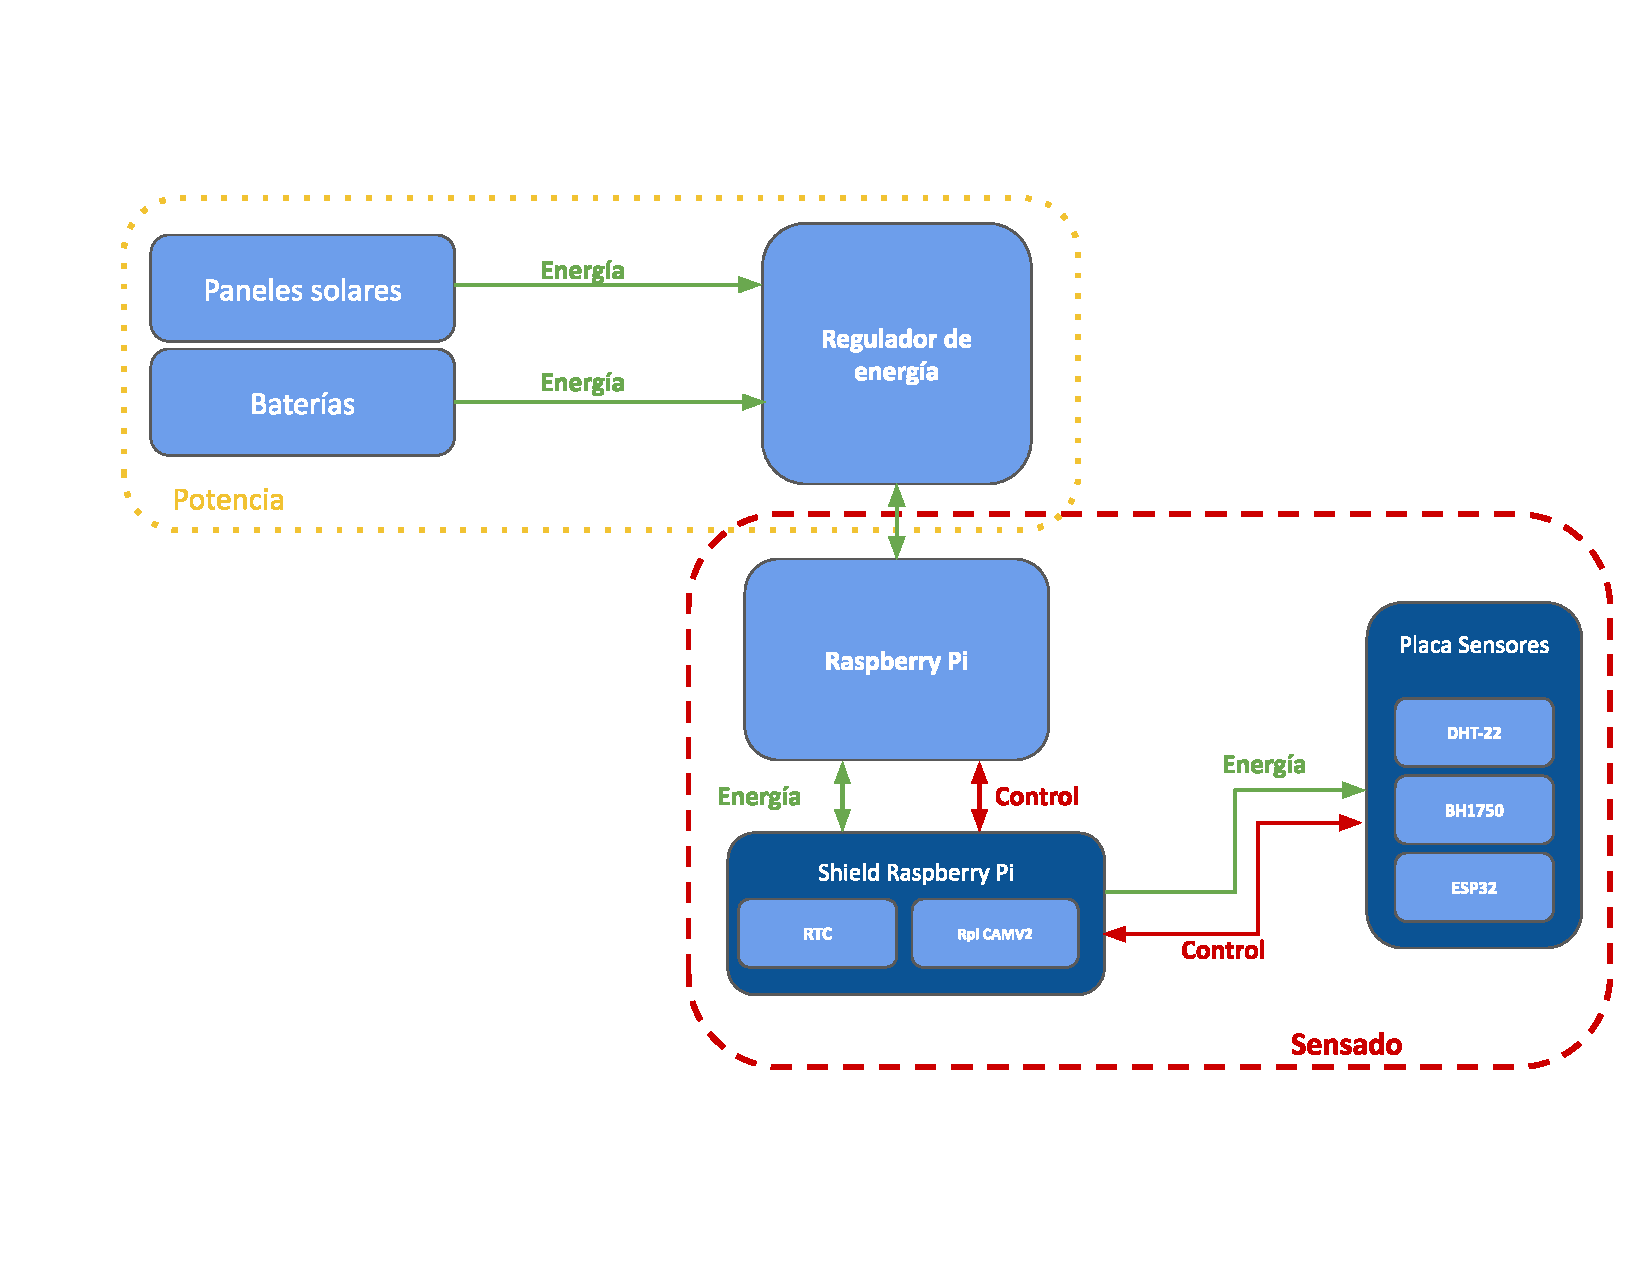
\includegraphics[width=0.7\linewidth]{ImagenesIngenieria de Detalle/DiagramaHardwareMarcado}
	\label{fig:diagrama_hardware}
	\caption{Diagrama en bloques del sistema de hardware.}
\end{figure}
La etapa de potencia es el conjunto de elementos necesarios para proveer de energ\'ia a toda la electr\'onica del proyecto.

El cargador es la etapa que se encarga, como su nombre indica realizar al carga inal\'ambrica de la UBM.

Y la de sensado se encarga de la medici\'on de las variables f\'isicas y de su correcto almacenamiento, teniendo en cuenta que esto implica un conocimiento preciso de la hora.



\Subsubsection{Descripción Detallada de cada Bloque}
\input{../Ingenieria de Detalle/Hardware/Descripción detallada de cada bloque.tex}

\Subsubsection{Detalles de Selección y Cálculo de los Elementos Circuitales de cada Bloque}
\label{sec:calc_potencias}
\input{../Ingenieria de Detalle/Hardware/Detalles de selección.tex}

\Subsubsection{Plan de Pruebas de cada Módulo}
El plan de pruebas corresponde a las descritas en [\ref{sec:BancoDePruebas}].
Para el uso correcto de los módulos se tuvieron en cuenta los siguientes aspectos:
\begin{itemize}
	\item Definir un estado predeterminado del Bus $I^2C$ mediante \textit{pullups}.
	\item El uso de capacitores de desacople
	\item Para el módulo RTC, el integrado DS1307 requiere $5 \ V$ para funcionar correctamente, por lo que para que sea compatible con la lógica de $3.3 \ V$ de la \rspi, se realiza un cambio en el esquemático al remover dos resistores del módulo.
\end{itemize}

\begin{figure}[H]
	\centering
	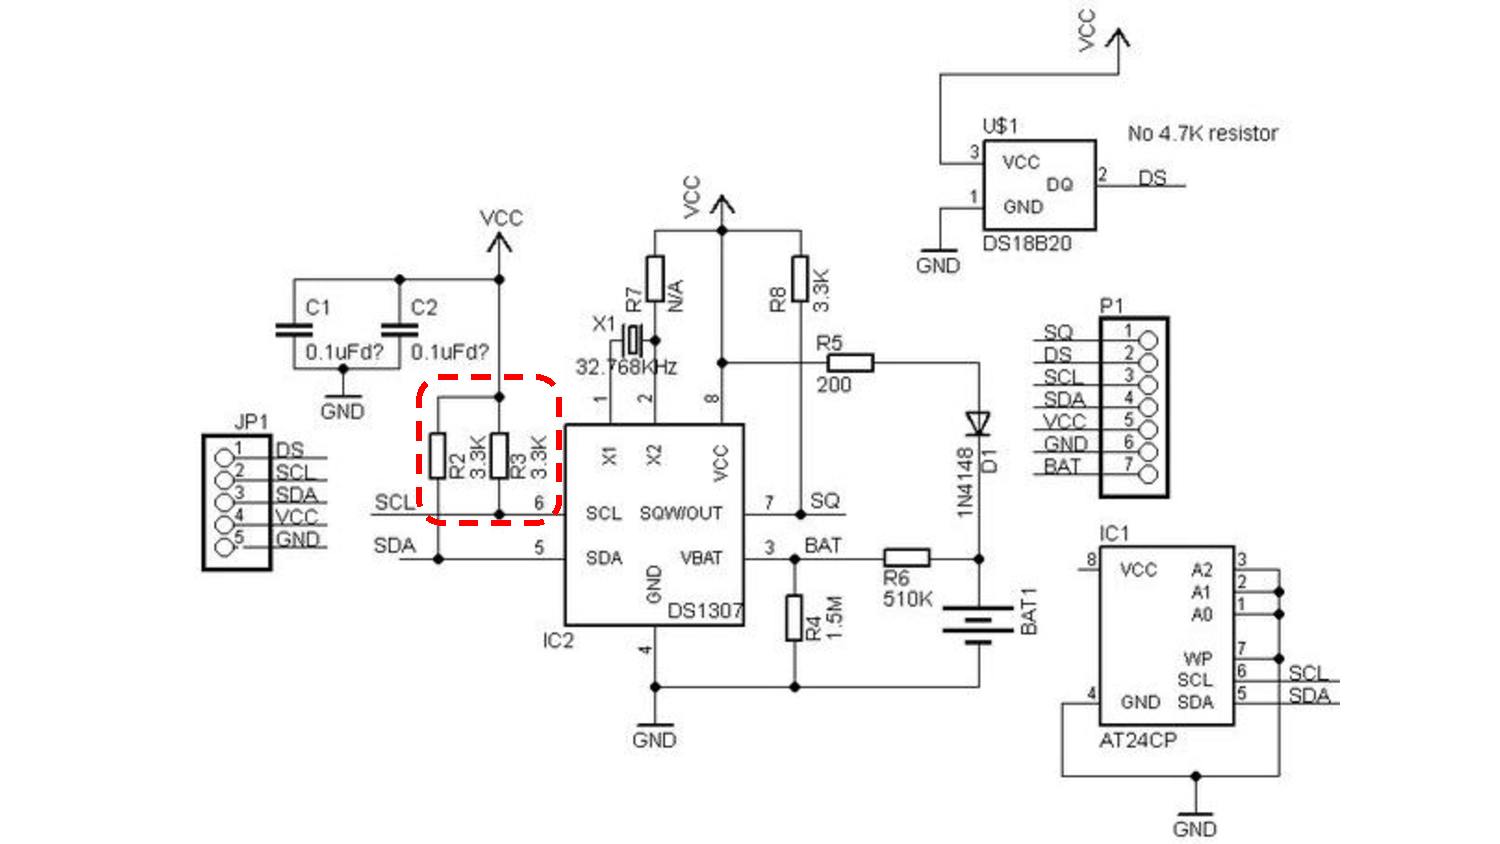
\includegraphics[width=0.9\linewidth,page=1]{ImagenesIngenieria de detalle/rtcTinySchematic}
	\caption{Esquemático RTC-Tiny.}
	\label{fig:RTCSchematic}
\end{figure}

Con este cambio se quita la referencia a $5 \ V$ del bus en el módulo. Por lo que la lógica queda en el rango de $3.3 \ V$ a $5 \ V$. Cabe destacar que utilizar los niveles lógicos de $3.3 \ V$ son compatibles con el integrado $DS1307$




\Subsection{Software}

\Subsubsection{Central de Control}
El centro de control, compuesto por una Raspberry-Pi, utiliza una distribución de Linux Server. Esto se debe a que no es de interés contar con una interfaz gráfica y es importante reservar espacio para almacenar los datos obtenidos desde los sensores y la cámara. 
Prescindir de la interfaz gráfica también permite ahorrar potencia dado que se apaga el puerto HDMI.

% TODO: \usepackage{graphicx} required
\begin{figure}[H]
	\centering
	\includegraphics[width=0.7\linewidth]{"../Ingenieria de Detalle/ImagenesIngenieria de Detalle/rpi_with_board"}
	\caption{Placa de desarrollo empleada.}
	%\label{fig:rpiwithboard}
\end{figure}



Se desarrollo la lógica de control utilizando el lenguaje de programación Python. Su rico ecosistema de paquetes nos permiten utilizar los diversos sensores y manejar las bases de datos.

% TODO: \usepackage{graphicx} required
\begin{figure}[H]
	\centering
	\includegraphics[width=0.7\linewidth]{"../Ingenieria de Detalle/ImagenesIngenieria de Detalle/python-logo@2x"}
	\caption{Lenguaje empleado para el control del proyecto.}
	%\label{fig:python-logo2x}
\end{figure}












\Subsubsection{Configuración Remota}
La configuración de la R-Pi se realiza de forma remota mediante SSH (secure shell).
Dado que el proyecto apunta a ser escalable y tener más de un nido operativo, se buscó una forma de configurar la R-Pi manera automática y replicable. Para ello se utiliza una herramienta de automatización llamada Ansible. Esta nos permite guardar sobre archivos de texto las configuraciones que necesita la R-Pi.

% TODO: \usepackage{graphicx} required
\begin{figure}[H]
	\centering
	\includegraphics[width=0.2\linewidth]{"../Ingenieria de Detalle/ImagenesIngenieria de Detalle/Ansible_logo"}
	\caption{Tecnología de automatización Ansible.}
	\label{fig:ansiblelogo}
\end{figure}
















%\Subsubsection{Eventos Periodicos}
%Durante la duración del proyecto la base de control deberá ejecutar una serie de acciones que se repetirán en el tiempo a intervalos de regulares. Para poder orquestrar estas actividades se hace uso de la utilidad nativa de Linux, los cronjobs. 
Utilizar esta actividad es ventajosa por sobre el método clásico de generar un único script que se encargue de todo. De esta forma evitamos un punto de falla que pondría en riesgo la ejecución de las demás acciones. 

% TODO: \usepackage{graphicx} required
%\begin{figure}[H]
%	\centering
%	\includegraphics[width=0.7\linewidth]{"../Ingenieria de Detalle/ImagenesIngenieria de Detalle/cron"}
%	\caption{Estructura de un cronjob.}
%	\label{fig:cron}
%\end{figure}

Por lo tanto, según los intervalos pre-establecidos se ejecutaran diferentes tareas. A continuación se detallan las acciones que se ejecutaran de forma periódica  
\begin{itemize}
	\item Encendido de la antena BLE durante el día.
	\item Reinicio periódico cada ocho horas.
	\item Apagado y encendido del \textit{server}. 
\end{itemize}



\Subsubsection{Diagrama de Estados y Flujogramas}
En este pasaje se habla sobre el diagrama de estados del sistema. El objetivo de este consiste en representar el funcionamiento de la lógica que se encuentra en Node-Red.

Cabe aclarar que por cuestiones de practicidad, en la Imagen (\ref{fig:diagrama_de_estados}) se simbolizan con nodos rojos, la interacción que el usuario tenga con la interfaz gráfica. Estos nodos representan los datos que se ingresan en el servidor por parte del cliente. Es decir, una comunicación unidireccional de la persona hacia el nido.

\begin{figure}[H]
	\centering	
	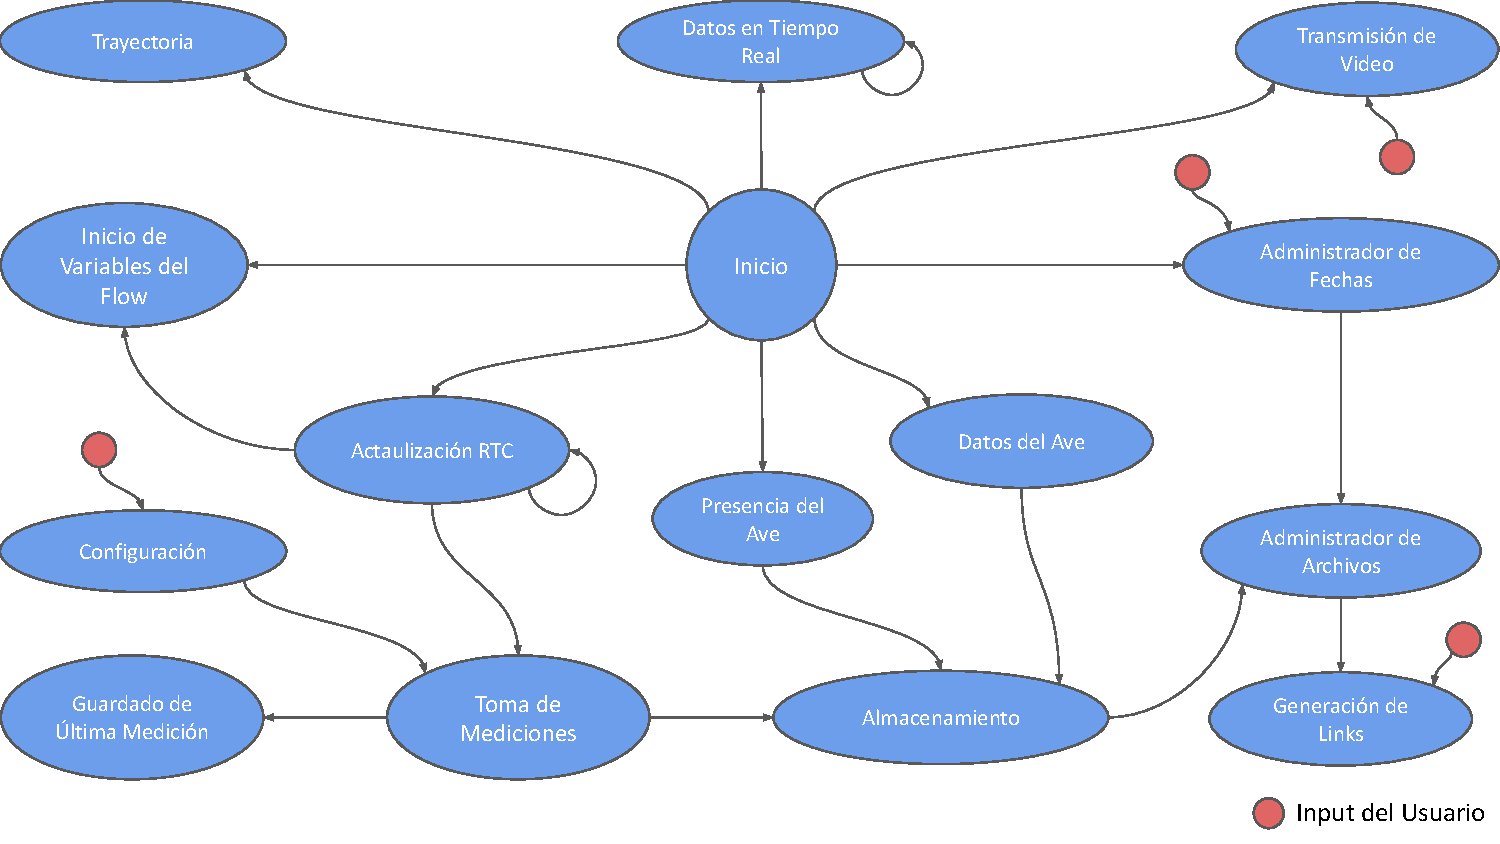
\includegraphics[width=\textwidth, page=1]{ImagenesIngenieria de Detalle/FlowChartNodeRed.pdf}	
	\caption{Diagrama de estados.}
	\label{fig:diagrama_de_estados}
\end{figure}

El nodo \textit{Inicio} es el principal. Si bien es el más simple, es el más importante porque inicia todo el sistema y su configuración. Este estado se ocupa de mandar distintos tipos de señales de arranque. Estas varían dependiendo del tipo de inicio que se busca determinar, distinguiendo así tres versiones distintas:
\begin{itemize}
	\item \textit{Init:} esta señal se envía cuando se inicia el servidor o cuando se realiza un cambio en los nodos mediante el usuario de administrador.
	\item \textit{F5:} se envía esta indicación cuando el usuario actualiza la página a la que tiene acceso.
	\item \textit{Init And F5:} esta es una combinación de las dos anteriores. El objetivo de esta es simplificar el esquema del sistema al momento de conectar los distintos estados y manejar su comunicación.
\end{itemize}

El siguiente estado en cuando a importancia es el de \textit{Actualización RTC}. Este es un nodo que se ocupa de leer el periférico de RTC y actualizar el valor dentro de Node-Red de manera periódica.

Con una de sus salidas se ocupa de inicializar las demás variables que se emplean en el servidor llamando a \textit{Inicio de Variables del Flow}. Es importante aclarar que las variables del flow son del tipo globales, es decir, cada nodo puede leerlas y modificarlas. Por cuestión de orden se asignó un estado propio para asignar valores por defecto y garantizar un correcto funcionamiento desde el arranque.

Con la salida faltante se comunica con el estado de \textit{Toma de Mediciones}. Como su nombre lo indica, se ocupa de verificar si ha transcurrido el intervalo de tiempo requerido con respecto a la última medición realizada. En caso afirmativo, se realiza la medición y luego informa a \textit{Guardado de Última Medición}, el cual actualiza la fecha y hora de este dato. Si bien \textit{Inicio de Variables del Flow} configura un intervalo por defecto para cada variable, \textit{Configuración} brinda la posibilidad de que el usuario cambie esos intervalos, manteniéndose en un margen de entre 5 minutos a 1 hora.

Con otra de las salidas del estado de \textit{Toma de Mediciones} se indica al nodo de \textit{Almacenamiento} de guardar el dato determinado. La razón por la cual \textit{Almacenamiento} tiene una salida es porque debe informar a \textit{Administración de Archivos} que hay datos nuevos. Este a su vez se ocupa de verificar cuáles de todos lo datos que posee deben ser mostrados al usuario. 

Esa decisión se encuentra regida en función de intervalos de tiempos, los cuales se determinan por una fecha inicial y final. Por defecto, \textit{Variables del Flow} asigna como día inicial y final la fecha en la cual se haya inicializado el servidor. Sumado a eso, \textit{Administrador de Fechas} se ocupa de brindarle al usuario la posibilidad de cambiar dicho período y de informar al \textit{Administración de Archivos} de dicho cambio.

El estado \textit{Generación de Links} se encarga de cargar los archivos adecuados para ser descargados y brindar al usuario acceso a estos.

\textit{Datos del Ave} obtiene los datos que se encuentran en la mochila del ave, para luego facilitárselos a \textit{Almacenamiento}. De una forma similar, \textit{Presencia del Ave} se ocupa de detectar si el ave se encuentra en el entorno del nido, mostrarlo en pantalla.

Su conexión con el estado de \textit{Almacenamiento} se da a que se guarda esta base de datos en la memoria de la R-Pi para aliviar el peso que debe soportar el servidor. Es por ello que estos a pesar de que el nodo que se ocupa de almacenar datos no brinda estos a \textit{Administrador de Archivos} ya que no es de interés que el usuario tenga acceso a la descarga de estos.

El nodo de \textit{Transmisión de Video} muestra en pantalla una transmisión en tiempo real del nido. Este se activa cuando el usuario lo solicite. Si bien es posible reiniciarlo y finalizarlo a voluntad, para evitar un uso excedido de dicha cualidad, y así evitar también una sobrecarga, el video se termina luego de 5 minutos de transmisión.

\textit{Datos en Tiempo Real} toma una medida de luminosidad, temperatura y humedad de manera periódica. Para evitar un uso excesivo de memoria, estos datos se superponen. El objetivo de este es mostrar al usuario en tiempo real las condiciones por dentro del nido.

Por último, el nodo de \textit{Trayectoria} se ocupa de mostrar la posición del ave en el entorno de medición de la red de seguimiento.

%\Subsubsection{Análisis de complejidad}
%\input{../Ingenieria de Detalle/Software/Análisis de complejidad.tex}

\Subsubsection{Descripción de Subrutinas}
\input{../Ingenieria de Detalle/Software/Descripción de subrutinas.tex}

%\Subsubsection{Listado de Elementos del Código}
%\TBD

%\Subsubsection{Plan de Prueba de Módulos y de Depuración de Software}
%El plan de pruebas corresponde a las descritas en [\ref{sec:BancoDePruebas}].
Para el uso correcto de los módulos se tuvieron en cuenta los siguientes aspectos:
\begin{itemize}
	\item Definir un estado predeterminado del Bus $I^2C$ mediante \textit{pullups}.
	\item El uso de capacitores de desacople
	\item Para el módulo RTC, el integrado DS1307 requiere $5 \ V$ para funcionar correctamente, por lo que para que sea compatible con la lógica de $3.3 \ V$ de la \rspi, se realiza un cambio en el esquemático al remover dos resistores del módulo.
\end{itemize}

\begin{figure}[H]
	\centering
	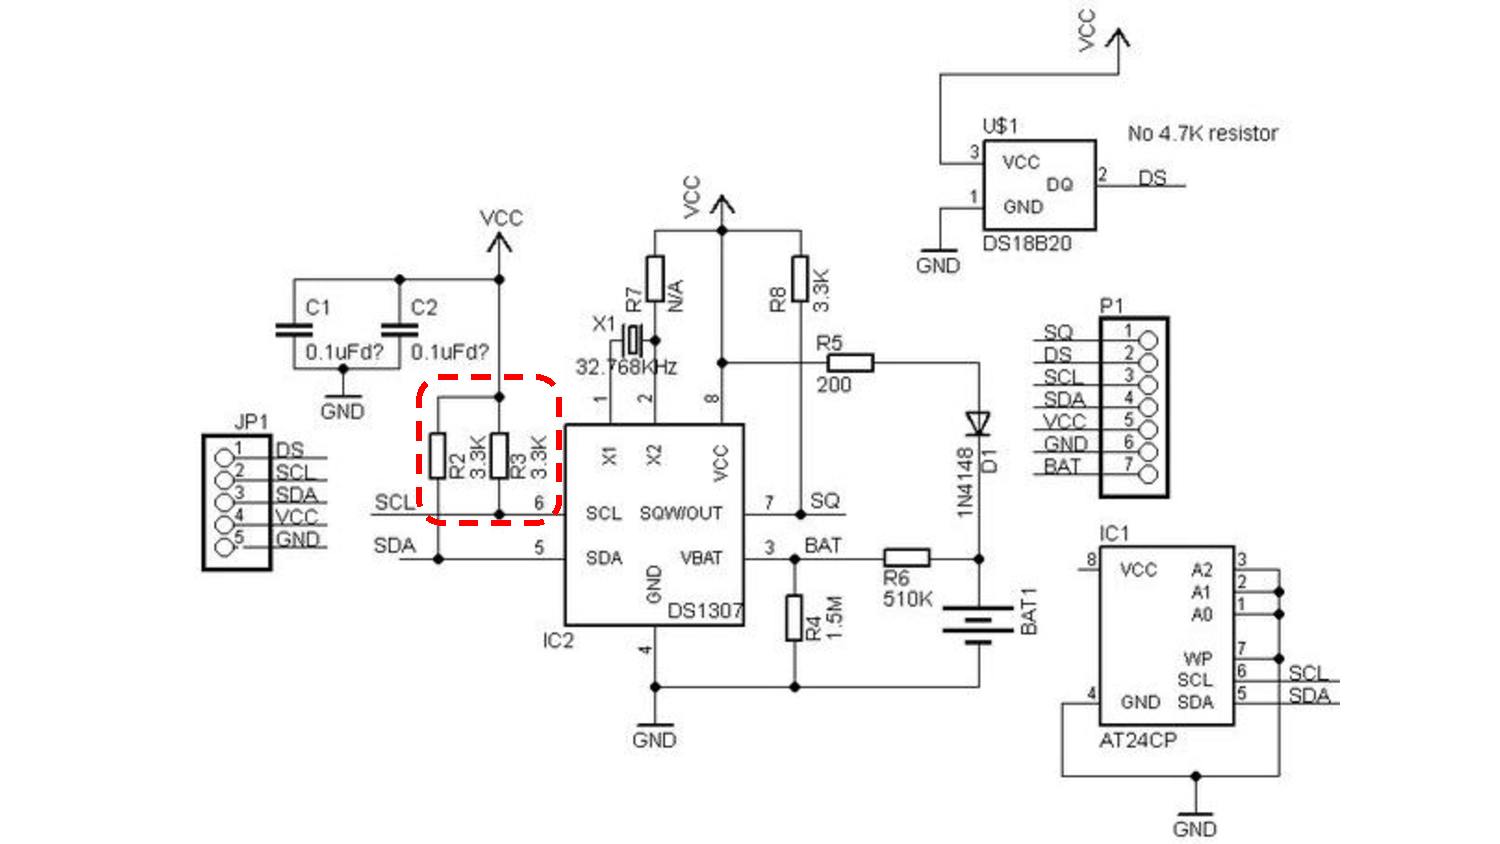
\includegraphics[width=0.9\linewidth,page=1]{ImagenesIngenieria de detalle/rtcTinySchematic}
	\caption{Esquemático RTC-Tiny.}
	\label{fig:RTCSchematic}
\end{figure}

Con este cambio se quita la referencia a $5 \ V$ del bus en el módulo. Por lo que la lógica queda en el rango de $3.3 \ V$ a $5 \ V$. Cabe destacar que utilizar los niveles lógicos de $3.3 \ V$ son compatibles con el integrado $DS1307$




\Subsubsection{Interfaz Gráfica de Usuario}
Para el desarrollo de la GUI, se valió del uso de \textbf{Node-Red}, software que permite el desarrollo de servicios online. Node-Red, mediante un sistema de nodos y sumado a la programación en JavaScript, permite generar una página web en una red local, lo cual cumple la función de interfaz con el usuario.

El sistema de edición y desarrollo de la GUI puede ser accedido a través de un navegador, de la misma manera que la interfaz del usuario. Para evitar que el usuario o alguna persona no deseada acceda a esta sección, se emplea un link privado, el cual es confidencial y no es publicado. También se vale de un sistema de autenticación que emplea la interfaz gráfica, creando un usuario de administrador.
\begin{figure}[H]
	\centering
	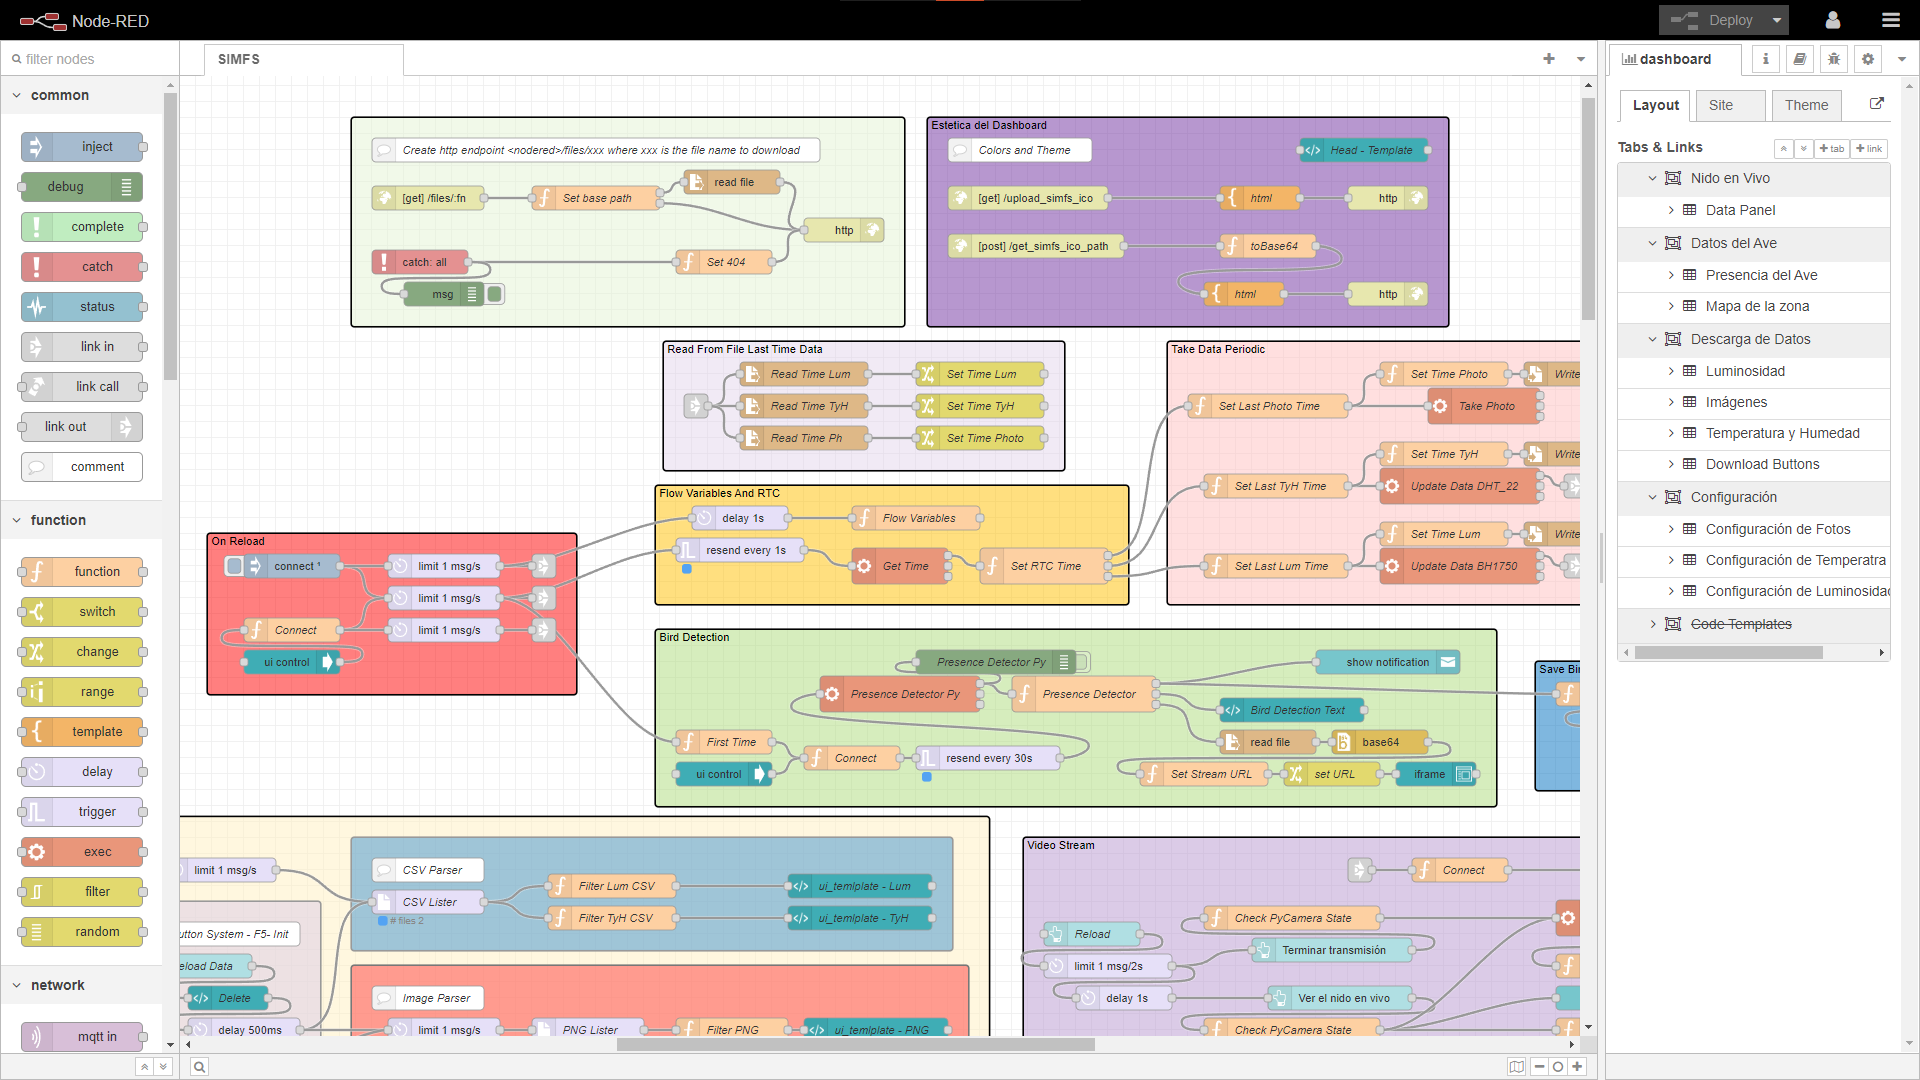
\includegraphics[width=0.9\linewidth]{ImagenesIngenieria de Detalle/Node-Red-Flow}
	\label{fig:node_red_flow}
	\caption{Flujo de nodos del servidor.}
\end{figure}

Dado que este servidor se encuentra corriendo en la R-Pi, al conectarse a la red de esta, se puede acceder a la página mencionada, donde se brindaran varias funcionalidades adicionales a las descargas básicas de los datos requeridos.

La interfaz gráfica a la cual el usuario tiene acceso posee distintas pestañas, donde cada una brinda un parámetro diferente. En la primer pestaña es posible ver las mediciones realizadas de luminosidad, temperatura y humedad en tiempo real. Además como el sistema detecta la presencia del ave, se muestra si este se encuentra dentro del nido o no. Por último se brinda al usuario la posibilidad de ver la una trasmisión en tiempo real del nido por dentro.
\begin{figure}[H]
\centering
    	\minipage{0.49\textwidth}
        	\centering
        	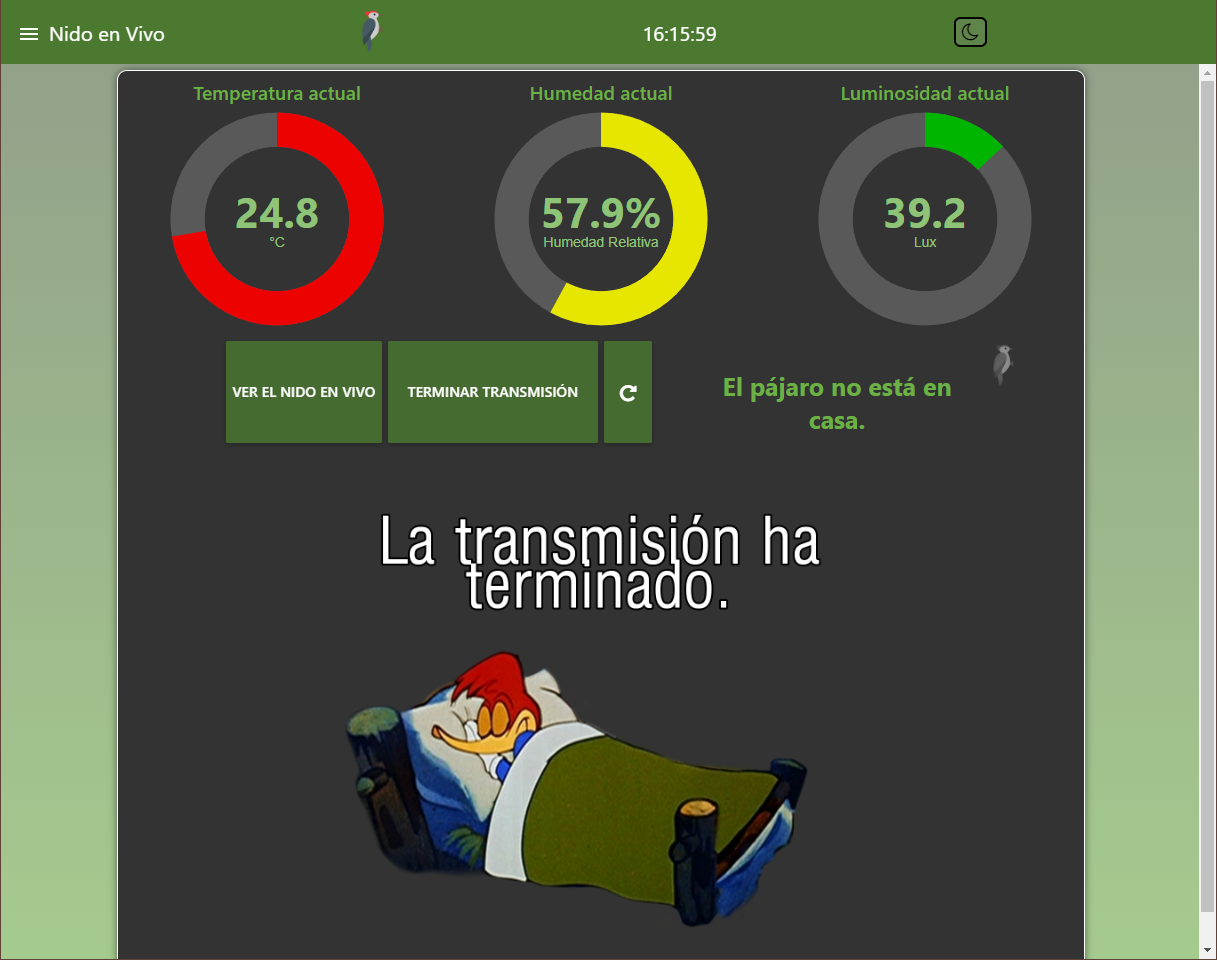
\includegraphics[width=\linewidth]{ImagenesIngenieria de Detalle/Node-Red-Live-Dark}		
			\caption{Interfaz con usuario versión oscura.}
			\label{fig:front_end_dark}
        \endminipage\hfill
        \minipage{0.49\textwidth}
        	\centering
        	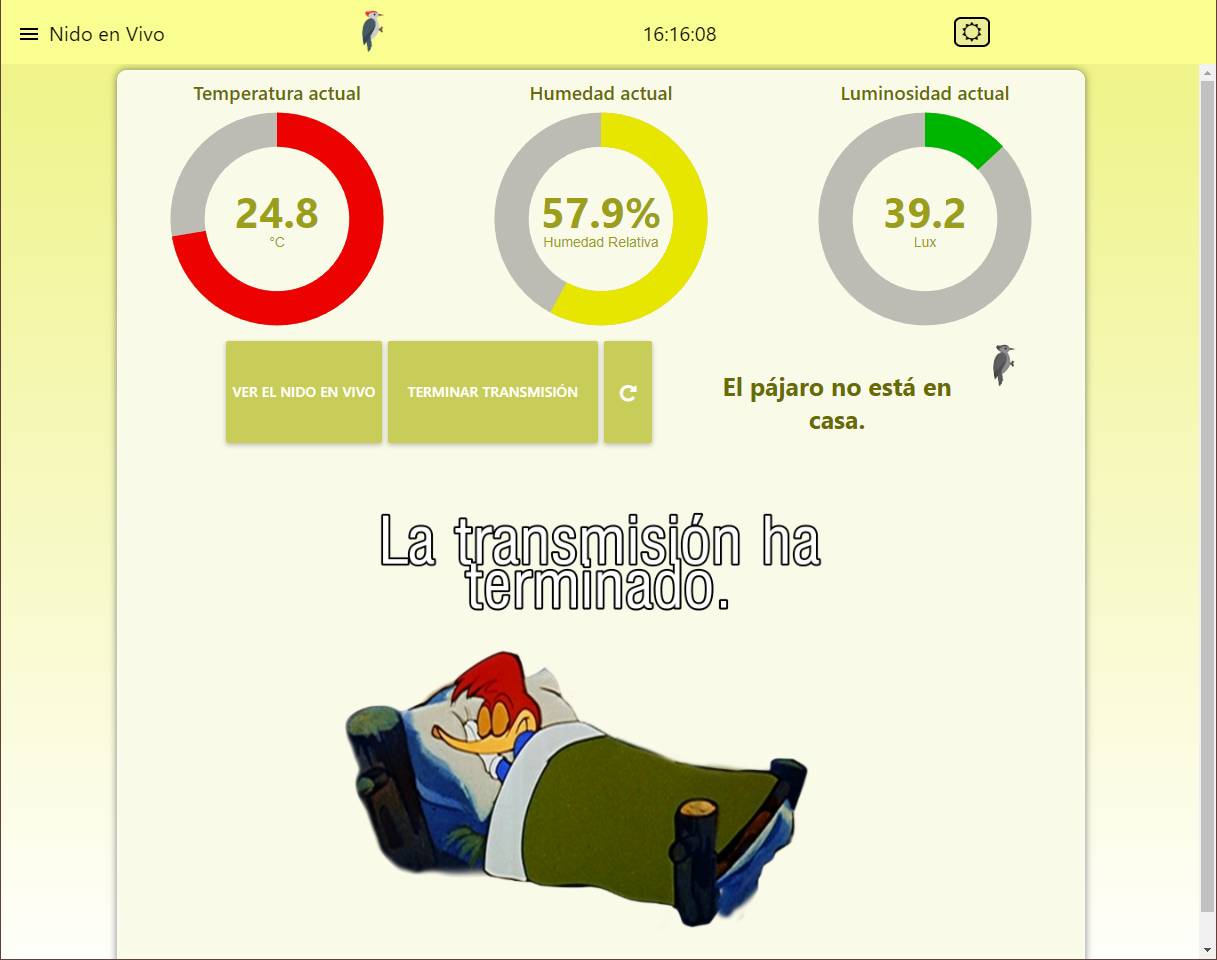
\includegraphics[width=\linewidth]{ImagenesIngenieria de Detalle/Node-Red-Live-Light}				\caption{Interfaz con usuario versión clara.}
			\label{fig:front_end_light}
        \endminipage
	\caption{Página del servidor a la cual accede el usuario.}
	\label{fig:node_red_live}
\end{figure}

En la segunda pestaña, es posible ver datos propios del ave, referidos a su posición. El primero muestra en un gráfico si el ave se ha encontrado dentro o fuera del nido durante un lapso de 24 horas, siendo posible seleccionar el día del cual se quiere ver los datos. Las zonas verdes denotan su estadía en el nido, mientras que las rijas su ausencia. Se muestra también cuanto tiempo duró cada intervalo. El segundo gráfico muestra el recorrido que ha realizado el ave en el entorno del nido en tiempo real.
\begin{figure}[H]
	\centering
    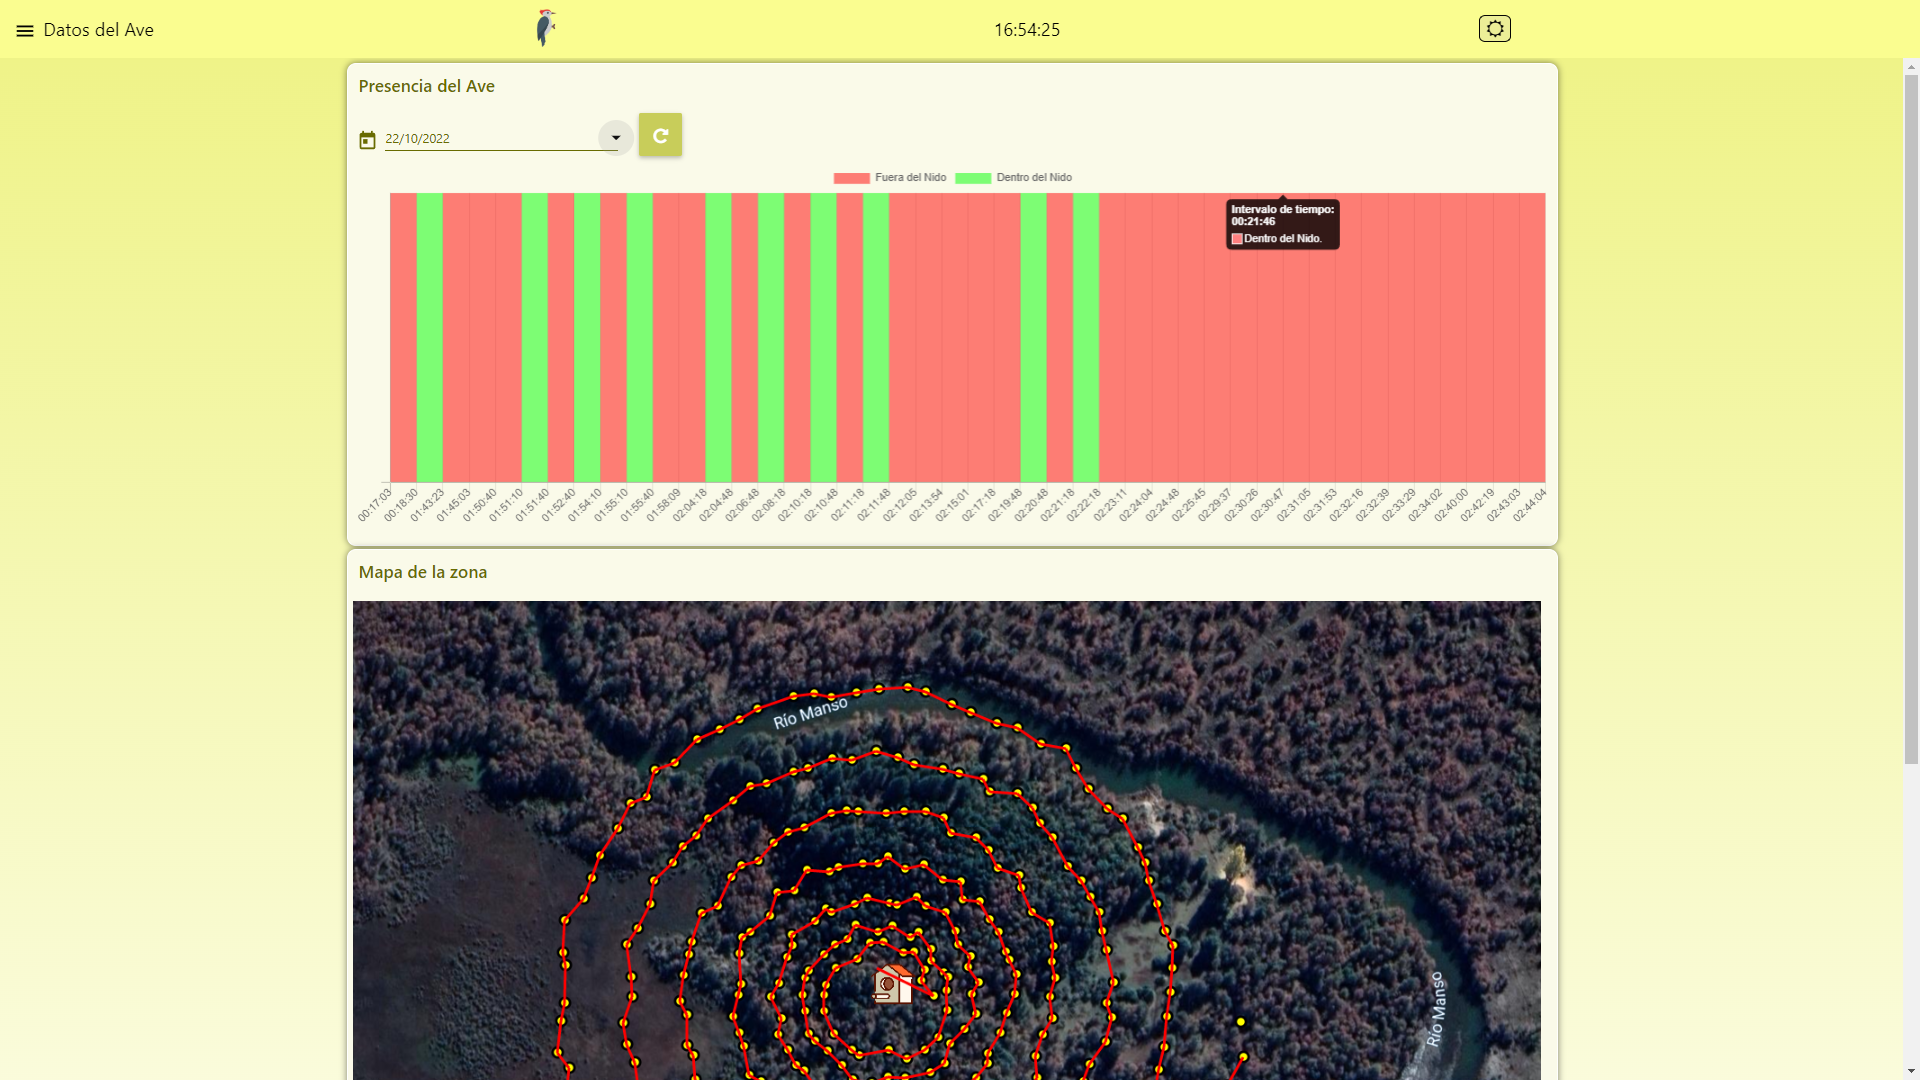
\includegraphics[width=0.7\linewidth]{ImagenesIngenieria de Detalle/Node-Red-Bird-Data}	
	\caption{Datos de presencia y posición del ave.}
	\label{fig:node_red_bird}
\end{figure}

La tercer pestaña es la más importante en cuanto a los requisitos del proyecto. En esta se presentan links de descarga para los datos obtenidos del nido y aquellos provistos por la unidad del pájaro. El usuario puede seleccionar el intervalo de tiempo en el cual desea obtener los datos.

Es posible descargar archivos del formato \quotes{csv} para los datos de luminosidad, temperatura y humedad, \quotes{png} si se desea descargar imágenes de forma individual o \quotes{zip} para el todo el conjunto de fotos mostradas.
\begin{figure}[H]
	\centering
    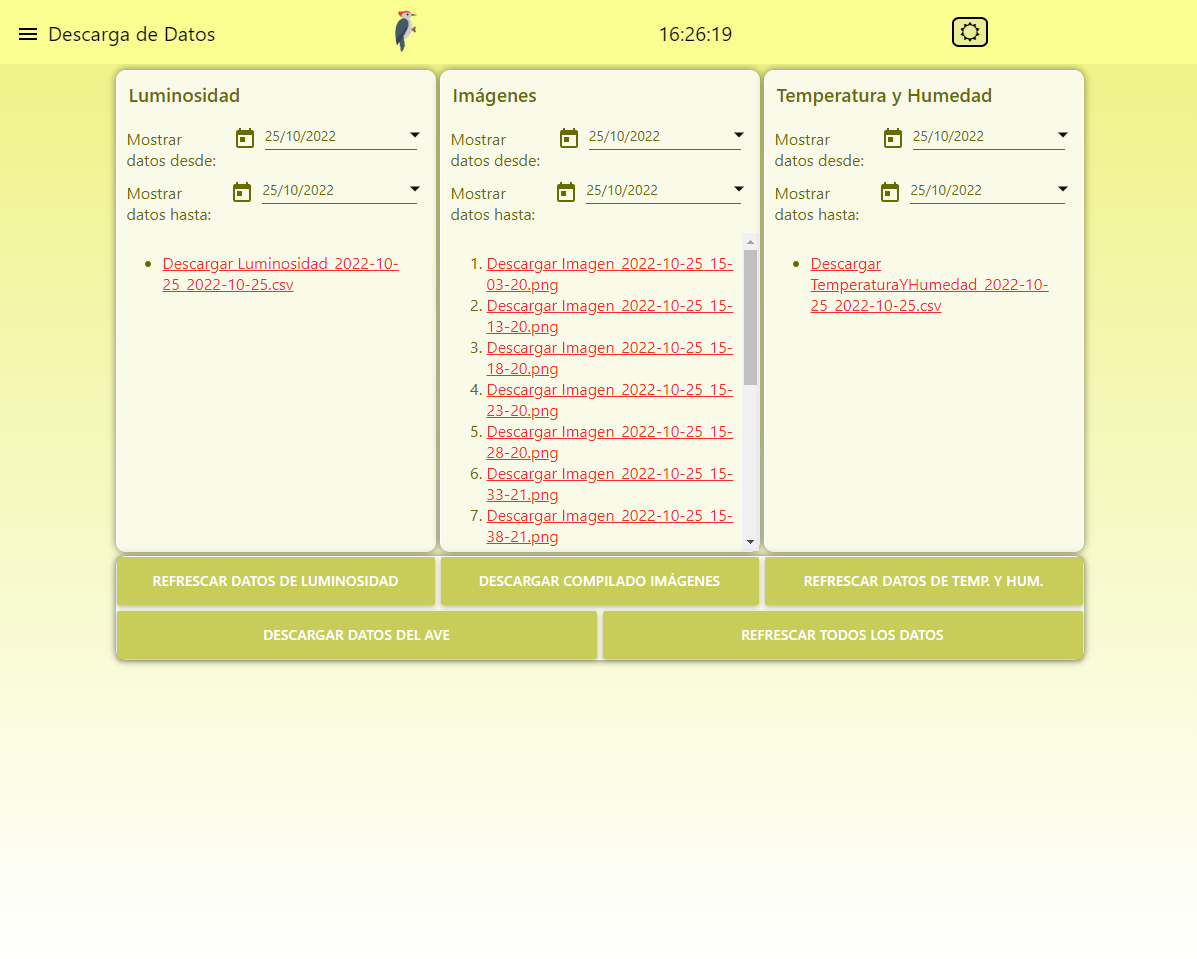
\includegraphics[width=0.7\linewidth]{ImagenesIngenieria de Detalle/Node-Red-Download}	
	\caption{Descarga de datos almacenados.}
	\label{fig:node_red_download}
\end{figure}

La cuarta y última pestaña le brinda al usuario cierto margen de configuración de la toma de datos. Estas opciones le permiten modificar el intervalo de cada medición, es decir cada cuanto tiempo se desea tomar una medición de las variables de interés o cada cuanto se desea tomar una foto.
\begin{figure}[H]
	\centering
    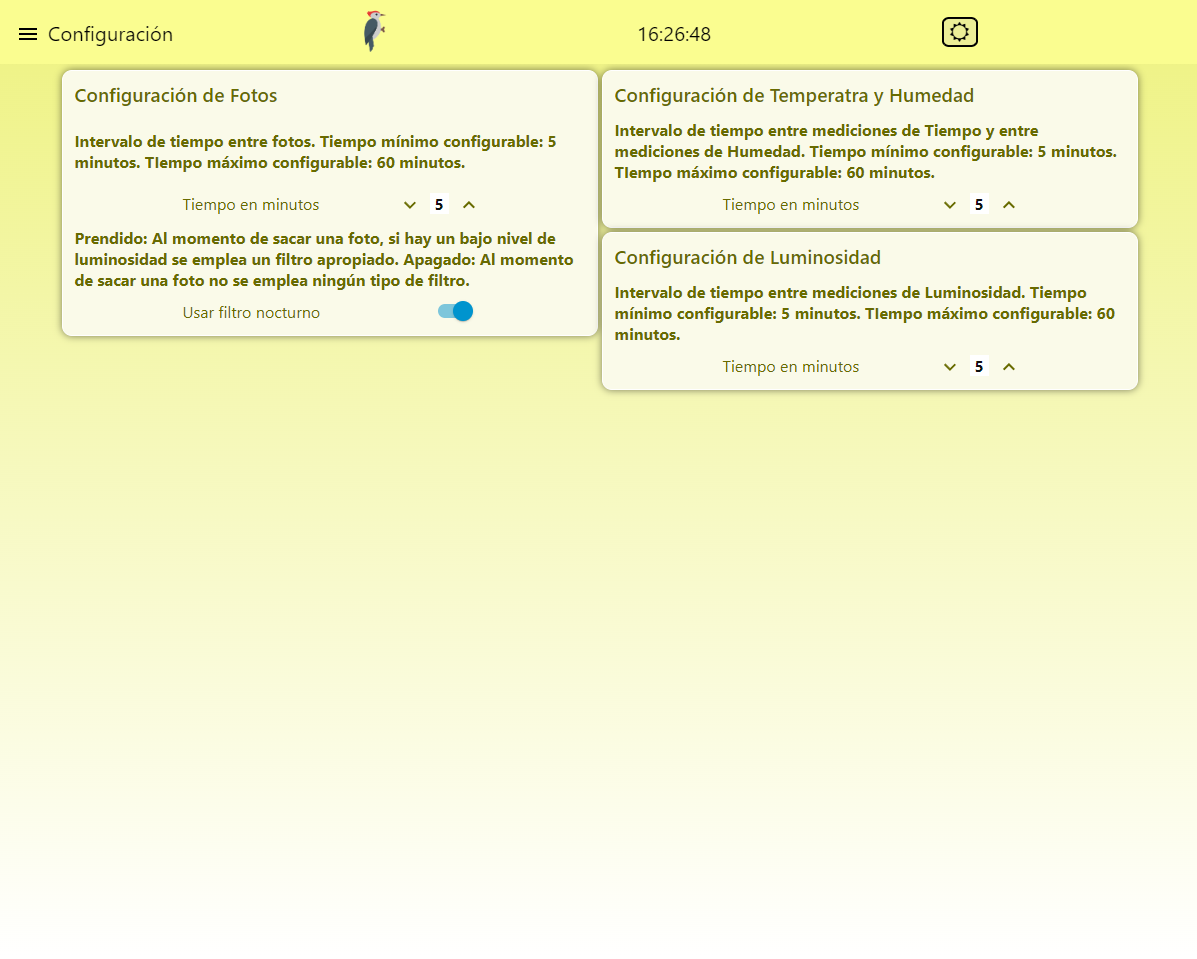
\includegraphics[width=0.7\linewidth]{ImagenesIngenieria de Detalle/Node-Red-Bird-Config}	
	\caption{Configuración de la interfaz gráfica.}
	\label{fig:node_red_config}
\end{figure}

También es posible determinar si se desea o no emplear un filtro en la cámara al momento tomar fotos, considerando el nivel luminosidad. En caso de que dicha variable posea un valor bajo se emplea el filtro mejorando así la luminosidad de la foto.
\begin{figure}[H]
\centering
    	\minipage{0.49\textwidth}
        	\centering
        	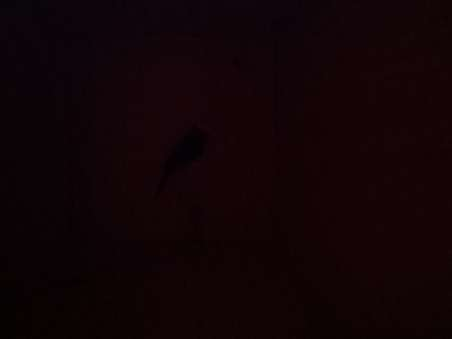
\includegraphics[width=\linewidth]{ImagenesIngenieria de Detalle/ImagenDevSF_2}		
			\caption{Foto tomada sin filtro de luminosidad.}
			\label{fig:foto_camara_sf}
        \endminipage\hfill
        \minipage{0.49\textwidth}
        	\centering
        	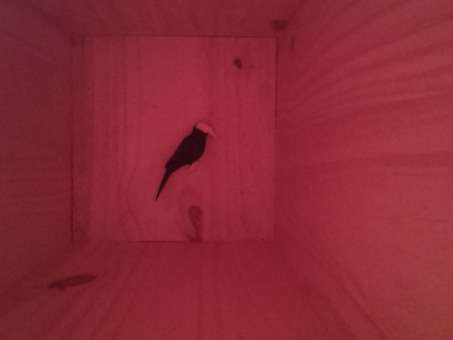
\includegraphics[width=\linewidth]{ImagenesIngenieria de Detalle/ImagenDevCF_2}					\caption{Foto tomada con filtro de luminosidad.}
			\label{fig:foto_camara_cf}
        \endminipage
	\caption{Comparación entre el uso del filtro de luminosidad.}
	\label{fig:foto_camara_filtro}
\end{figure}

Cabe destacar que de la misma forma que se considera un usuario de administrador, la GUI cuenta con una cuenta con contraseña para brindarle acceso al usuario y así evitar el uso de cualquier persona que consiga conexión a la red.

%\end{document}


\Section{Construcción del Prototipo}
%\documentclass[a4paper]{article}
%\usepackage[utf8]{inputenc}
\usepackage[spanish, es-tabla, es-noshorthands]{babel}
\usepackage[table,xcdraw,dvipsnames]{xcolor}
\usepackage[a4paper, footnotesep=1.25cm, headheight=1.25cm, top=2.54cm, left=2.54cm,
 bottom=2.54cm, right=2.54cm]{geometry}
%\geometry{showframe}
 \usepackage[normalem]{ulem}
 \useunder{\uline}{\ul}{}

%VERIFICAR EL HEAD Y EL FOOT EN
%https://ctan.dcc.uchile.cl/macros/latex/contrib/geometry/geometry.pdf

%Paquetes varios:
\usepackage{verbatimbox}

%\usepackage{wrapfig}			%Wrap figure in text
\usepackage[export]{adjustbox}	%Move images
\usepackage{changepage}			%Move tables
\usepackage{todonotes}

\usepackage{tikz}
\usepackage{amsmath}
\usepackage{amsfonts}
\usepackage{amssymb}
\usepackage{float}
\usepackage[graphicx]{realboxes}
\usepackage{caption}
\usepackage{subcaption}
\usepackage{multicol}
\usepackage{multirow}
\setlength{\doublerulesep}{\arrayrulewidth}
%\usepackage{booktabs}

\usepackage{array}
\newcolumntype{C}[1]{>{\centering\let\newline\\\arraybackslash\hspace{0pt}}m{#1}}
%\usepackage[american]{circuitikz}
\usetikzlibrary{calc}
\usepackage{fancyhdr}
\usepackage{units} 

\usepackage{colortbl}
%\usepackage{sectsty}
%\usepackage{unicode-math}

%FONTS (IMPORTANTE): Compilar en XeLaTex o LuaLaTeX
\usepackage{anyfontsize}	%Font size
\usepackage{fontspec}		%Font type
%Si sigue sin andar comentar \usepackage[utf8]{inputenc}
%https://ctan.dcc.uchile.cl/macros/unicodetex/latex/fontspec/fontspec.pdf
%https://www.overleaf.com/learn/latex/XeLaTeX

%Path para imagenes para trabajar en subarchivos
\graphicspath{{../Resumen/}{../Referencias/}{../Apendice/}{../Descripción de la Empresa/}{../Tareas del Alumno/}{../Conclusiones/}{../Herramientas Empleadas/}}

%Definiciones de nuevos comandos y colores
%COLORES:
\definecolor{AzulFoot}{rgb}{0.682,0.809,0.926}	%RGB	%{174,206,235}
\definecolor{AzulInfo}{rgb}{0.180,0.455,0.710}	%RGB	%{46,116,181}
\definecolor{AzulTable}{rgb}{0.302,0.507,0.871}	%RGB	%{68,114,196}
\definecolor{PName}{rgb}{0.353,0.353,0.353}		%RGB	%{90,90,90}
\definecolor{mygreen}{rgb}{28,172,0} % color values Red, Green, Blue
\definecolor{mylilas}{rgb}{170,55,241}

%Change Font Size

% #1 = size, #2 = text
\newcommand{\setparagraphsize}[2]{{\fontsize{#1}{6}\selectfont#2 \par}}		%Cambia el size de todo el parrafo
\newcommand{\setlinesize}[2]{{\fontsize{#1}{6}\selectfont#2}}				%Cambia el font de una oración

%IMAGE IN TABLE:			%Ejemplo: \includeintable{.3}{ImagenesFactibilidad/pend}
\renewcommand\fbox{\fcolorbox{white}{white}}
\setlength{\fboxrule}{0pt}	%padding thickness
\setlength{\fboxsep}{4pt}	%border thickness
\newcommand{\includeintable}[2]{	
	\fbox{
		\begin{minipage}{#1\textwidth}
        	\includegraphics[width=\linewidth]{#2}
    	\end{minipage}
	}
}

%LINK IN REF
\newcommand{\reflink}[1]{		%LINK
	\href{#1}{#1}
}

%NOTAS:
\newcommand{\note}[1]{		%RED BIG NOTE (TODO)
	\begin{center}
		\huge{ \textcolor{red}{#1} }
	\end{center}
}

\newcommand{\lnote}[1]{{\fontsize{14}{6}\selectfont\textcolor{green}{#1}}}	%Notas pequeñas

\newcommand{\observacion}[2]{  \ifnumequal{1}{#1}{ { \todo[inline,backgroundcolor=red!25,bordercolor=red!100]{\textbf{Observación: #2}} } }{  }  }

\newcommand{\red}[1]{\textcolor{red}{#1}}

\newcommand{\TBD}{\textcolor{red}{(TBD) }}
\newcommand{\tbd}{\textcolor{red}{(TBD) }}

\newcommand{\TBC}{\textcolor{red}{(TBC) }}
\newcommand{\tbc}{\textcolor{red}{(TBC) }}

\newcommand{\quotes}[1]{``#1''}
\newcommand{\q}[1]{``#1''}

\newcommand{\ip}{192.168.0.10:1880}
\newcommand{\ipadmin}{192.168.0.10:1880/admin}

% Comandos para agregar elementos en tablas de acronimos y definiciones
\newcommand{\addacronym}[2]{\textbf{#1} & \begin{tabular}[l]{@{}l@{}}#2\end{tabular} \\ \hline}

% tabItem
\newcommand{\tabitem}{~~\llap{\textbullet}~~}


\usepackage{hyperref}
\hypersetup{
    colorlinks=true,
    linkcolor=black,
    filecolor=magenta,      
    urlcolor=AzulInfo,
    citecolor=AzulInfo,    
}

%Configuración del header y del footer:
\usepackage{etoolbox}
\pagestyle{fancy}
\fancyhf{}
\rfoot{\thepage}
\renewcommand{\footrulewidth}{4pt}
\renewcommand{\headrulewidth}{0pt}
\patchcmd{\footrule}{\hrule}{\color{AzulFoot}\hrule}{}{}

%Código en el informe
%% IMPORTANTE:
% Verificar que esté \usepackage[dvipsnames]{xcolor}

%\usepackage{listingsutf8}
\usepackage{listings}

\renewcommand{\lstlistingname}{Código}

%LSTSET: Pone un recuadro y contador de linea en el codigo
\newcommand{\boxstyle}{
	\lstset{
		basicstyle=\sffamily\color{black},
		frame=single,
		numbers=left,
		numbersep=5pt,
		numberstyle=\color{gray},
		showspaces=false,
		showstringspaces=false
	}
}

\newcommand{\defaultstyle}{
	\lstset{
		basicstyle=\sffamily\color{white},
		frame=none,
		numbers=none,
		showspaces=true,
		showstringspaces=true
	}
}

\lstdefinelanguage{Kotlin}{
  captionpos=b,
  comment=[l]{//},
  commentstyle={\color{gray}\ttfamily},
  emph={filter, first, firstOrNull, forEach, lazy, map, mapNotNull, println},
  emphstyle={\color{OrangeRed}},
  identifierstyle=\color{black},
  keywords={!in, !is, abstract, actual, annotation, as, as?, break, by, catch, class, companion, const, constructor, continue, crossinline, data, delegate, do, dynamic, else, enum, expect, external, false, field, file, final, finally, for, fun, get, if, import, in, infix, init, inline, inner, interface, internal, is, lateinit, noinline, null, object, open, operator, out, override, package, param, private, property, protected, public, receiveris, reified, return, return@, sealed, set, setparam, super, suspend, tailrec, this, throw, true, try, typealias, typeof, val, var, vararg, when, where, while},
  keywordstyle={\color{NavyBlue}\bfseries},
  morecomment=[s]{/*}{*/},
  morestring=[b]",
  morestring=[s]{"""*}{*"""},
  ndkeywords={@Deprecated, @JvmField, @JvmName, @JvmOverloads, @JvmStatic, @JvmSynthetic, Array, Byte, Double, Float, Int, Integer, Iterable, Long, Runnable, Short, String, Any, Unit, Nothing},
  ndkeywordstyle={\color{BurntOrange}\bfseries},
  sensitive=true,
  stringstyle={\color{ForestGreen}\ttfamily},
}

\lstdefinelanguage{Swift}
{
  morekeywords={
    open,catch,@escaping,nil,throws,func,if,then,else,for,in,while,do,switch,case,default,where,break,continue,fallthrough,return,
    typealias,struct,class,enum,protocol,var,func,let,get,set,willSet,didSet,inout,init,deinit,extension,
    subscript,prefix,operator,infix,postfix,precedence,associativity,left,right,none,convenience,dynamic,
    final,lazy,mutating,nonmutating,optional,override,required,static,unowned,safe,weak,internal,
    private,public,is,as,self,unsafe,dynamicType,true,false,nil,Type,Protocol,
  },
  morecomment=[l]{//}, % l is for line comment
  morecomment=[s]{/*}{*/}, % s is for start and end delimiter
  morestring=[b]", % defines that strings are enclosed in double quotes
  breaklines=true,
  escapeinside={\%*}{*)},
  numbers=left,
  captionpos=b,
  breakatwhitespace=true,
  basicstyle=\linespread{1.0}\ttfamily, % https://tex.stackexchange.com/a/102728/129441
}

\definecolor{keyword}{HTML}{BA2CA3}
\definecolor{string}{HTML}{D12F1B}
\definecolor{comment}{HTML}{008400}

\newcommand{\swiftstyle}{
	\lstset{
  		language=Swift,
  		inputencoding=utf8x,
		extendedchars=\true,
	  	basicstyle=\ttfamily,
	  	showstringspaces=false, % lets spaces in strings appear as real spaces
  		columns=fixed,
  		keepspaces=true,
  		keywordstyle=\color{keyword},
  		stringstyle=\color{string},
  		commentstyle=\color{comment}
	}
}


%Como usarlo:

%\begin{lstlisting}[caption={Simple code listing.}, label={lst:example1}, language=Kotlin]
%// this is a simple code listing:
%println("hello kotlin from latex")
%\end{lstlisting}

%Si se corta en 2 páginas distintas:

%\vspace{1mm}
%\noindent{\begin{minipage}{\linewidth}
%\begin{lstlisting}[...]
%...
%\end{lstlisting}
%\end{minipage}}




\usepackage{titlesec}		%Para hacer las subsubsubsections

%Colores a los nombres de las secciones:
%\sectionfont{\color{AzulInfo}}  % sets color of sections
%\subsectionfont{\color{AzulInfo}}
%\subsubsectionfont{\color{AzulInfo}}

%PICTURES AND TABLE INDEX:
\newcommand{\Section}[1]{ \section{#1} 
	\phantomsection \setcounter{figure}{0} \setcounter{table}{0} \setcounter{lstlisting}{0}
		\renewcommand{\thetable}{\arabic{section}.\arabic{table}}
		\renewcommand{\thefigure}{\arabic{section}.\arabic{figure}}
		\renewcommand{\thelstlisting}{\arabic{section}.\arabic{lstlisting}}
}

\newcommand{\Subsection}[1]{ \subsection{#1}
	\phantomsection \setcounter{figure}{0} \setcounter{table}{0} \setcounter{lstlisting}{0}
		\renewcommand{\thetable}{\arabic{section}.\arabic{subsection}.\arabic{table}}
		\renewcommand{\thefigure}{\arabic{section}.\arabic{subsection}.\arabic{figure}}
		\renewcommand{\thelstlisting}{\arabic{section}.\arabic{subsection}.\arabic{lstlisting}}
}

\newcommand{\Subsubsection}[1]{ \subsubsection{#1} 
	\phantomsection \setcounter{figure}{0} \setcounter{table}{0}  \setcounter{lstlisting}{0}
		\renewcommand{\thetable}{\arabic{section}.\arabic{subsection}.\arabic{subsubsection}.\arabic{table}}
		\renewcommand{\thefigure}{\arabic{section}.\arabic{subsection}.\arabic{subsubsection}.\arabic{figure}}
		\renewcommand{\thelstlisting}{\arabic{section}.\arabic{subsection}.\arabic{subsubsection}.\arabic{lstlisting}}
}

%Definición de subsubsubsection:
\titleclass{\subsubsubsection}{straight}[\subsection]

\newcounter{subsubsubsection}[subsubsection]
\renewcommand\thesubsubsubsection{\thesubsubsection.\arabic{subsubsubsection}}

\titleformat{\subsubsubsection}
  {\normalfont\normalsize\bfseries\color{AzulInfo}}{\thesubsubsubsection}{1em}{}	%Color de subsubsubsection
\titlespacing*{\subsubsubsection}
{0pt}{3.25ex plus 1ex minus .2ex}{1.5ex plus .2ex}

\makeatletter
\renewcommand\paragraph{\@startsection{paragraph}{5}{\z@}%
  {3.25ex \@plus1ex \@minus.2ex}%
  {-1em}%
  {\normalfont\normalsize\bfseries}}
\renewcommand\subparagraph{\@startsection{subparagraph}{6}{\parindent}%
  {3.25ex \@plus1ex \@minus .2ex}%
  {-1em}%
  {\normalfont\normalsize\bfseries}}
\def\toclevel@subsubsubsection{4}
\def\toclevel@paragraph{5}
\def\toclevel@paragraph{6}
\def\l@subsubsubsection{\@dottedtocline{4}{7em}{4em}}
\def\l@paragraph{\@dottedtocline{5}{10em}{5em}}
\def\l@subparagraph{\@dottedtocline{6}{14em}{6em}}
\makeatother

\setcounter{secnumdepth}{4}
\setcounter{tocdepth}{4}

%Subsubsubsection:
\newcommand{\Subsubsubsection}[1]{ \subsubsubsection{#1} 
	\phantomsection \setcounter{figure}{0} \setcounter{table}{0} \renewcommand{\thetable}{\arabic{section}.\arabic{subsection}.\arabic{subsubsection}.\arabic{subsubsubsection}.\arabic{table}} \renewcommand{\thefigure}{\arabic{section}.\arabic{subsection}.\arabic{subsubsection}.\arabic{subsubsubsection}.\arabic{figure}}
}

%Tamaño, color e identación de sección, subsección, subsubsección y subsubsubsección:
%La identación de las subsecciones está tambien en Index-cfg.tex para el toc, lot y lot en el index
\titleformat{\section}[block]{\fontsize{16}{6}\selectfont\bfseries\color{AzulInfo}}{\thesection.}{1em}{} 
\titleformat{\subsection}[block]{\hspace{2.5em}\fontsize{13}{6}\selectfont\color{AzulInfo}}{\thesubsection}{1em}{}
\titleformat{\subsubsection}[block]{\hspace{3.5em}\fontsize{12}{6}\selectfont\color{AzulInfo}}{\thesubsubsection}{1em}{}
\titleformat{\subsubsubsection}[block]{\hspace{4em}\fontsize{11}{6}\selectfont\color{AzulInfo}}{\thesubsubsubsection}{1em}{}

%Pone las refrencias en el indice
\usepackage[numbib, nottoc, notlot, notlof]{tocbibind}

%Pone toc, lof y lot en colores y elijo el titulo de estos
\addto\captionsspanish{
	\renewcommand\contentsname{Contenidos}
	\renewcommand\listfigurename{Lista de Figuras}
	\renewcommand\listtablename{Lista de Tablas}
}

%Agrega TOC al indice
\renewcommand{\tableofcontents}{
	\stepcounter{section}
	\addcontentsline{toc}{section}{\protect\numberline{\thesection}\textbf{Contenidos}}
	\tableofcontents
}

%Agrega LOF al indice
\renewcommand{\listoffigures}{
	\stepcounter{section}
	\addcontentsline{toc}{section}{\protect\numberline{\thesection}\textbf{Lista de Figuras}}
	\listoffigures
}

%Agrega LOT al indice
\renewcommand{\listoftables}{
	\stepcounter{section}
	\addcontentsline{toc}{section}{\protect\numberline{\thesection}\textbf{Lista de Tablas}}
	\listoftables
}

%Indices: cambio la separación de los numeros para que entren tablas y fotos
\usepackage{tocloft}
\setlength{\cftfignumwidth}{1.35cm}  % change numwidth from figures in lof
\setlength{\cfttabnumwidth}{1.35cm}  % change numwidth from tables in lot
\renewcommand{\cfttoctitlefont}{\Large\bfseries\color{AzulInfo}}
\renewcommand{\cftloftitlefont}{\Large\bfseries\color{AzulInfo}}
\renewcommand{\cftlottitlefont}{\Large\bfseries\color{AzulInfo}}

%Coloca lineas punteadas a las seciones en el TOC
\renewcommand{\cftsecleader}{\cftdotfill{\cftdotsep}}

%Items con bullets y no cuadrados
\renewcommand{\labelitemi}{\textbullet }


\Subsection{Prototipo Nido- Carga Bater\'ia}
Al momento de comenzar la construcci\'on del prototipo de nido, en el cual se validar\'a la carga inal\'ambrica se propusieron 4 requerimientos que deb\'ia cubrir.
\begin{enumerate}
\item Condiciones an\'alogas a las del nido real:
Para este item el enfoque que se toma es una visi\'on electromagnetica.
Un parámetro fundamental a definir es el ancho que tienen las paredes del nido prototipo. Se sabe que el menor valor que tiene la cavidad real es de 65mm \cite{ref:PaperValeriaOjeda}.

Mediante el uso de la Equación (\ref{eq:penetracion}) se calcula la profundidad de penetración de la onda electromagnética.
\begin{equation}
\delta \ = \ \frac{1}{\alpha} \ =\ \frac{1}{\sqrt{\pi f \mu \sigma}}
\label{eq:penetracion}
\end{equation}
Este valor simboliza la distancia que penetra la onda electromagn\'etica hasta ser atenuada en un 63$\%$
Para ello se sabe que los valores de las constantes son los siguientes:
\begin{itemize}
	\item Frecuencia $f = 915 \ MHz$.
	\item Permeabilidad magnética de la madera \cite{ref:permeabilidad_madera}: $\mu_{Madera} = 1.25663760 \ \mu \frac{Hy}{m}$.
	\item Conductividad de la madera \cite{ref:conductividad_madera}:$\sigma \approx 1 \ m\frac{S}{m}$.
\end{itemize}

Con los valores mencionados, reemplazando en la Ecuación (\ref{eq:penetracion}) se obtiene que $\delta = 526 \ mm$.
De este resultado se concluye que independientemente del espesor del proptipo, siempre que sea menor al real. La onda electromang\'etica no es atenuada a un 63$\%$ de su amplitud. Por lo que atraviesa tanto el arbol como el proptipo sin problemas.(Pensando en las paredes.)

Luego se procede a calcular el coeficiente de reflexión de la onda electromagnética. Para ello se sabe también que las permitividades de la madera y aire son:
\begin{itemize}
	\item $\varepsilon_{Madera} = 17.7 10^{-12} \ \frac{F}{m}$ \cite{ref:varepsilon_madera}.
	\item $\varepsilon_{Aire} = 8.8595003 10^{-12} \ \frac{F}{m}$
	\item $\mu_{Aire} = 1.25663753 \ \mu \frac{ Hy}{m}$ 
\end{itemize}

También se calcula la impedancia de la madera como:
\begin{equation}
	\eta_{Madera}=\sqrt{\frac{\mu_{Madera}}{\varepsilon_{Madera}}}
\end{equation}

Es así que el coeficiente de reflexión se calcula de la siguiente forma:
\begin{equation}
	\Gamma = \frac{\eta_2 - \eta_1  }{\eta_2 + \eta_1} = -0.1714
	\label{eq:reflexion_madera}
\end{equation}

Se observa en la Ecuación (\ref{eq:reflexion_madera}) que el resultado presenta un valor negativo. Lo que esto implica es una inversión de fase en la onda electromagnética reflejada respecto de la incidente. Esto implica una interferencia destructiva, para determinar las implicancias de esta interferencai se calcula la potencia de la onda reflejada, siendo esta $P_{ref} = |\Gamma|^2 = 0.029$. Es así que se nota que menos de un $3\%$ de la potencia sera reflejada. De esta forma se puede afirmar que no habrá una interferencia significativa con la transmisión original.
Finalmente cabe notar que el resultado del coeficiente de reflexi\'pm no depende del espesor. \'Unicamente de la impedancia de los medios. Por lo que de aqu\'i se concluye que el espesor de la madera no juega un papel significativo en el prototipo de nido.
\item Altura regulable:
La altura entre el receptor de potencia y el transmisor debe ser variable ebntre 30 y 64 cm debido a que no todos los nidos tienen la misma altura y asi se podra simular eso.
\item Sujeci\'on instrumental:
El proptipo debe brindar alguna manera de asegurar la electr\'onica al prototipo.
\item Conicimiento de la distancia entre el receptor y el transmisor de potencia:
Para ello utilizamos un sensor ultrasónico que estará montado en la parte interior de la tapa, con un display en la parte exterior. las mediciones y control del display se hará con un pequeño microcontrolador.(Cabe mencionar que este modulo de ultrasonido ser\'a utilizada \'unicamente en el prototipo, no con un ave real, debido a que se sabe que las aves son alteradas por dichas ondas de ultrasonido)
\end{enumerate} 
Con estos requerimientos cumplidos se diseño el prototipo de nido, con los planos especificados en (\ref{fig:Base_nido_plano}) (\ref{fig:Base_electronica_plano}) (\ref{fig:tapa_nido_plano}) y (\ref{fig:explotado_nido_plano})
\Subsection{Prototipo Mochila - Carga}
Para este prototipo se utliza la placa de desarrollo P1110 de energy harvesting. 
\TBC
\Subsection{Prototipo Mochila - Comunicaci\'on}
Para esto se utilizar\'a un m\'odulo BLE para transmitir un set de datos GPS de aproximadamente un peso de 2KBy y un pin l\'ogico que permita activar la recepci\'on de datos del lado del nido.




\Section{Validación del Prototipo}
%Para la validación del prototipo se emplean los mismos bancos de prueba mencionados en la Sección (\ref{sec:PlanValidacion}), ya que no existe una diferencia sustancial que implique la necesidad de alterar dichos ensayos.

\Subsection{Validación pruebas funcionales}

Se empieza por las pruebas de \textit{T-INT-FUN-01} y \textit{T-INT-FUN-02}. Ambas pruebas se realizan a la par, no solo porque comparten el mismo banco de pruebas, sino porque se emplea el mismo sensor calibrado para la corroboración. Este sensor es capaz de medir tanto temperatura como humedad.
\begin{figure}[H]
\centering
	\begin{subfigure}{0.39\textwidth}
    	\centering
        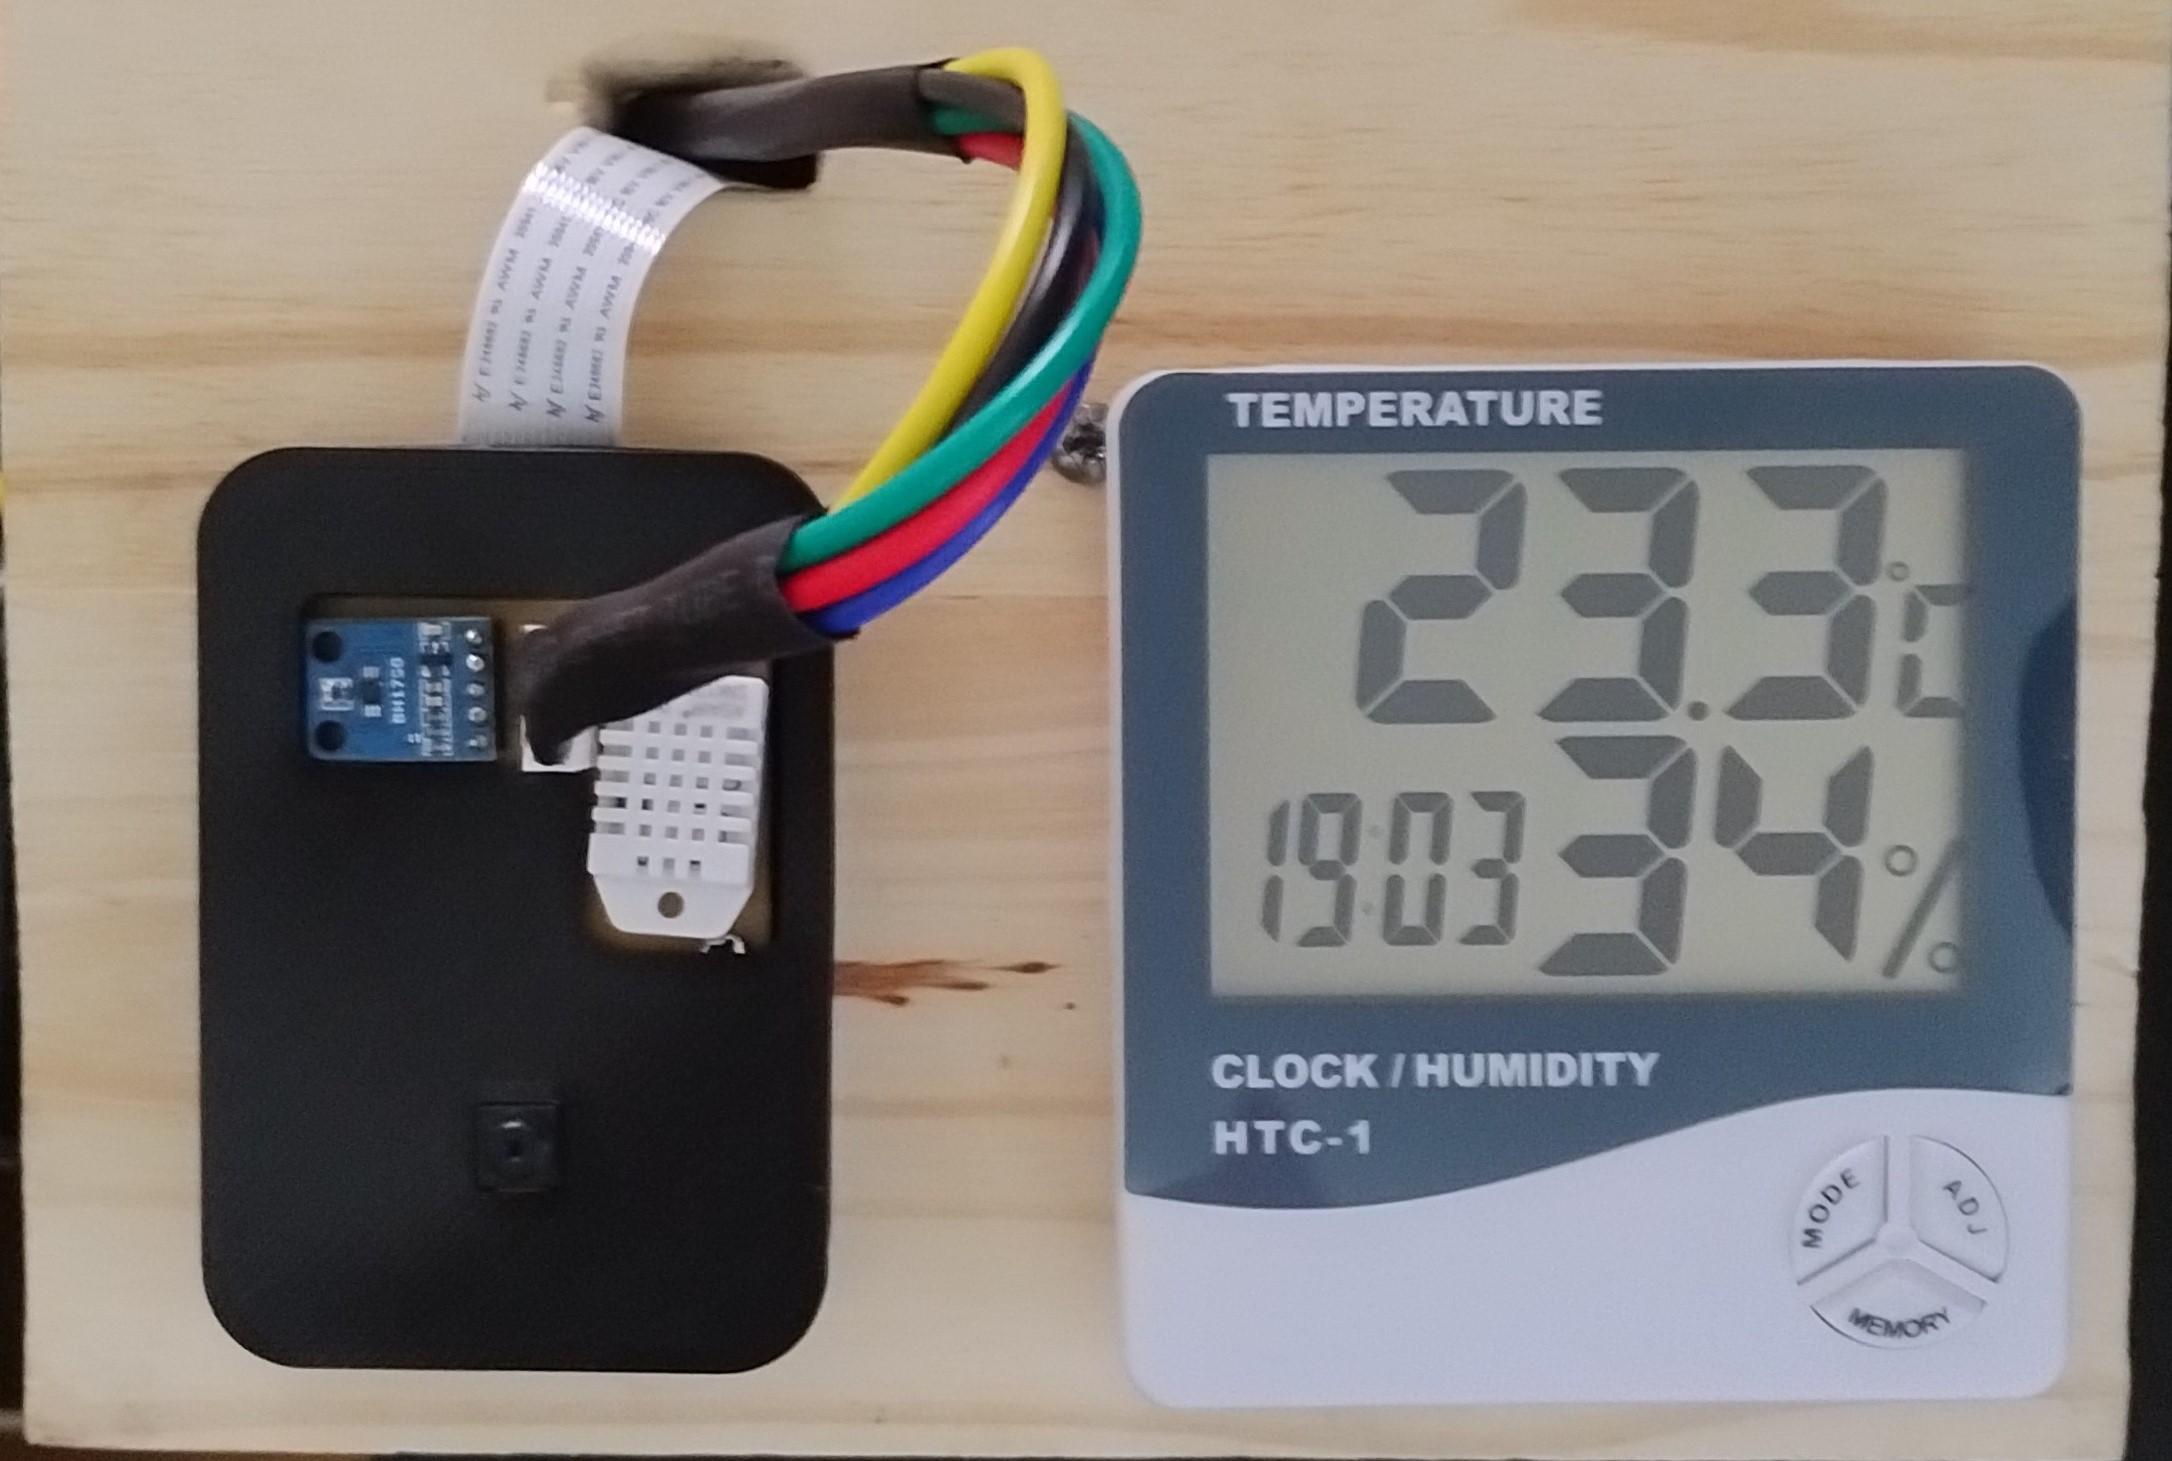
\includegraphics[width=\linewidth]{ImagenesValidacion del prototipo/T-INT-FUN-1-2-Medicion}		
		\caption{Sensores de comparación.}
	\end{subfigure}\hfill
    \begin{subfigure}{0.6\textwidth}
    	\centering
        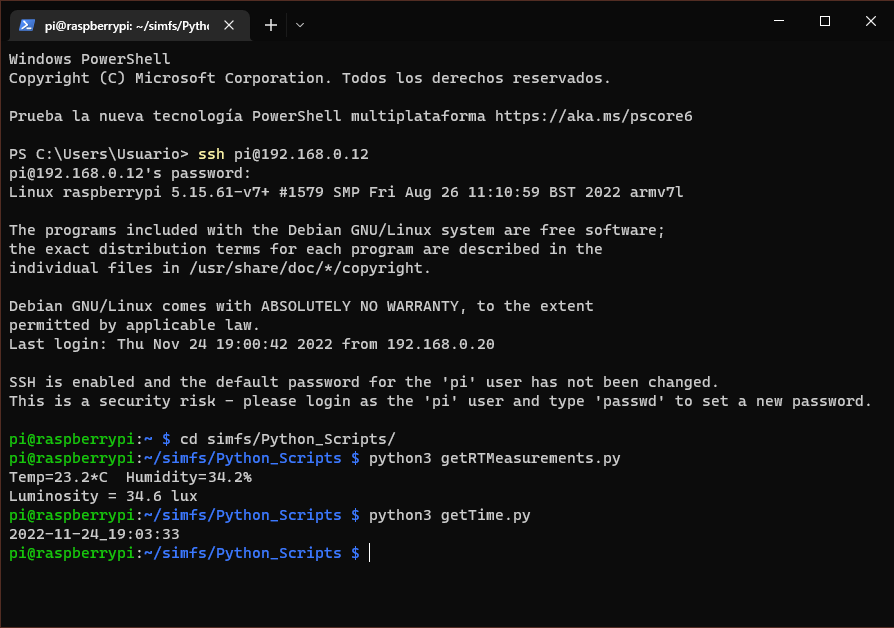
\includegraphics[width=\linewidth]{ImagenesValidacion del prototipo/T-INT-FUN-1-2}		
        \caption{Medición obtenida.}
	\end{subfigure}
	\caption{Validación de funcionalidad \textit{T-INT-FUN-01} y \textit{T-INT-FUN-02}.}
\end{figure}

De esta forma se verifica que los sensores se encuentran calibrados con un margen de error menor al máximo permitido (desviación máxima de $\pm \  0.5^o \ C$ y $\pm \ 2 \ \%$ respectivamente).

Para las validaciones del sensor de luminosidad se desarrollaron las pruebas acorde a \textit{T-INT-FUN-03}, obteniendo los resultados esperados para todos los casos, como se observa en la Figura (\ref{fig:valLum}).
\begin{figure}[H]
	\centering
    \begin{subfigure}{0.33\textwidth}
    	\centering
        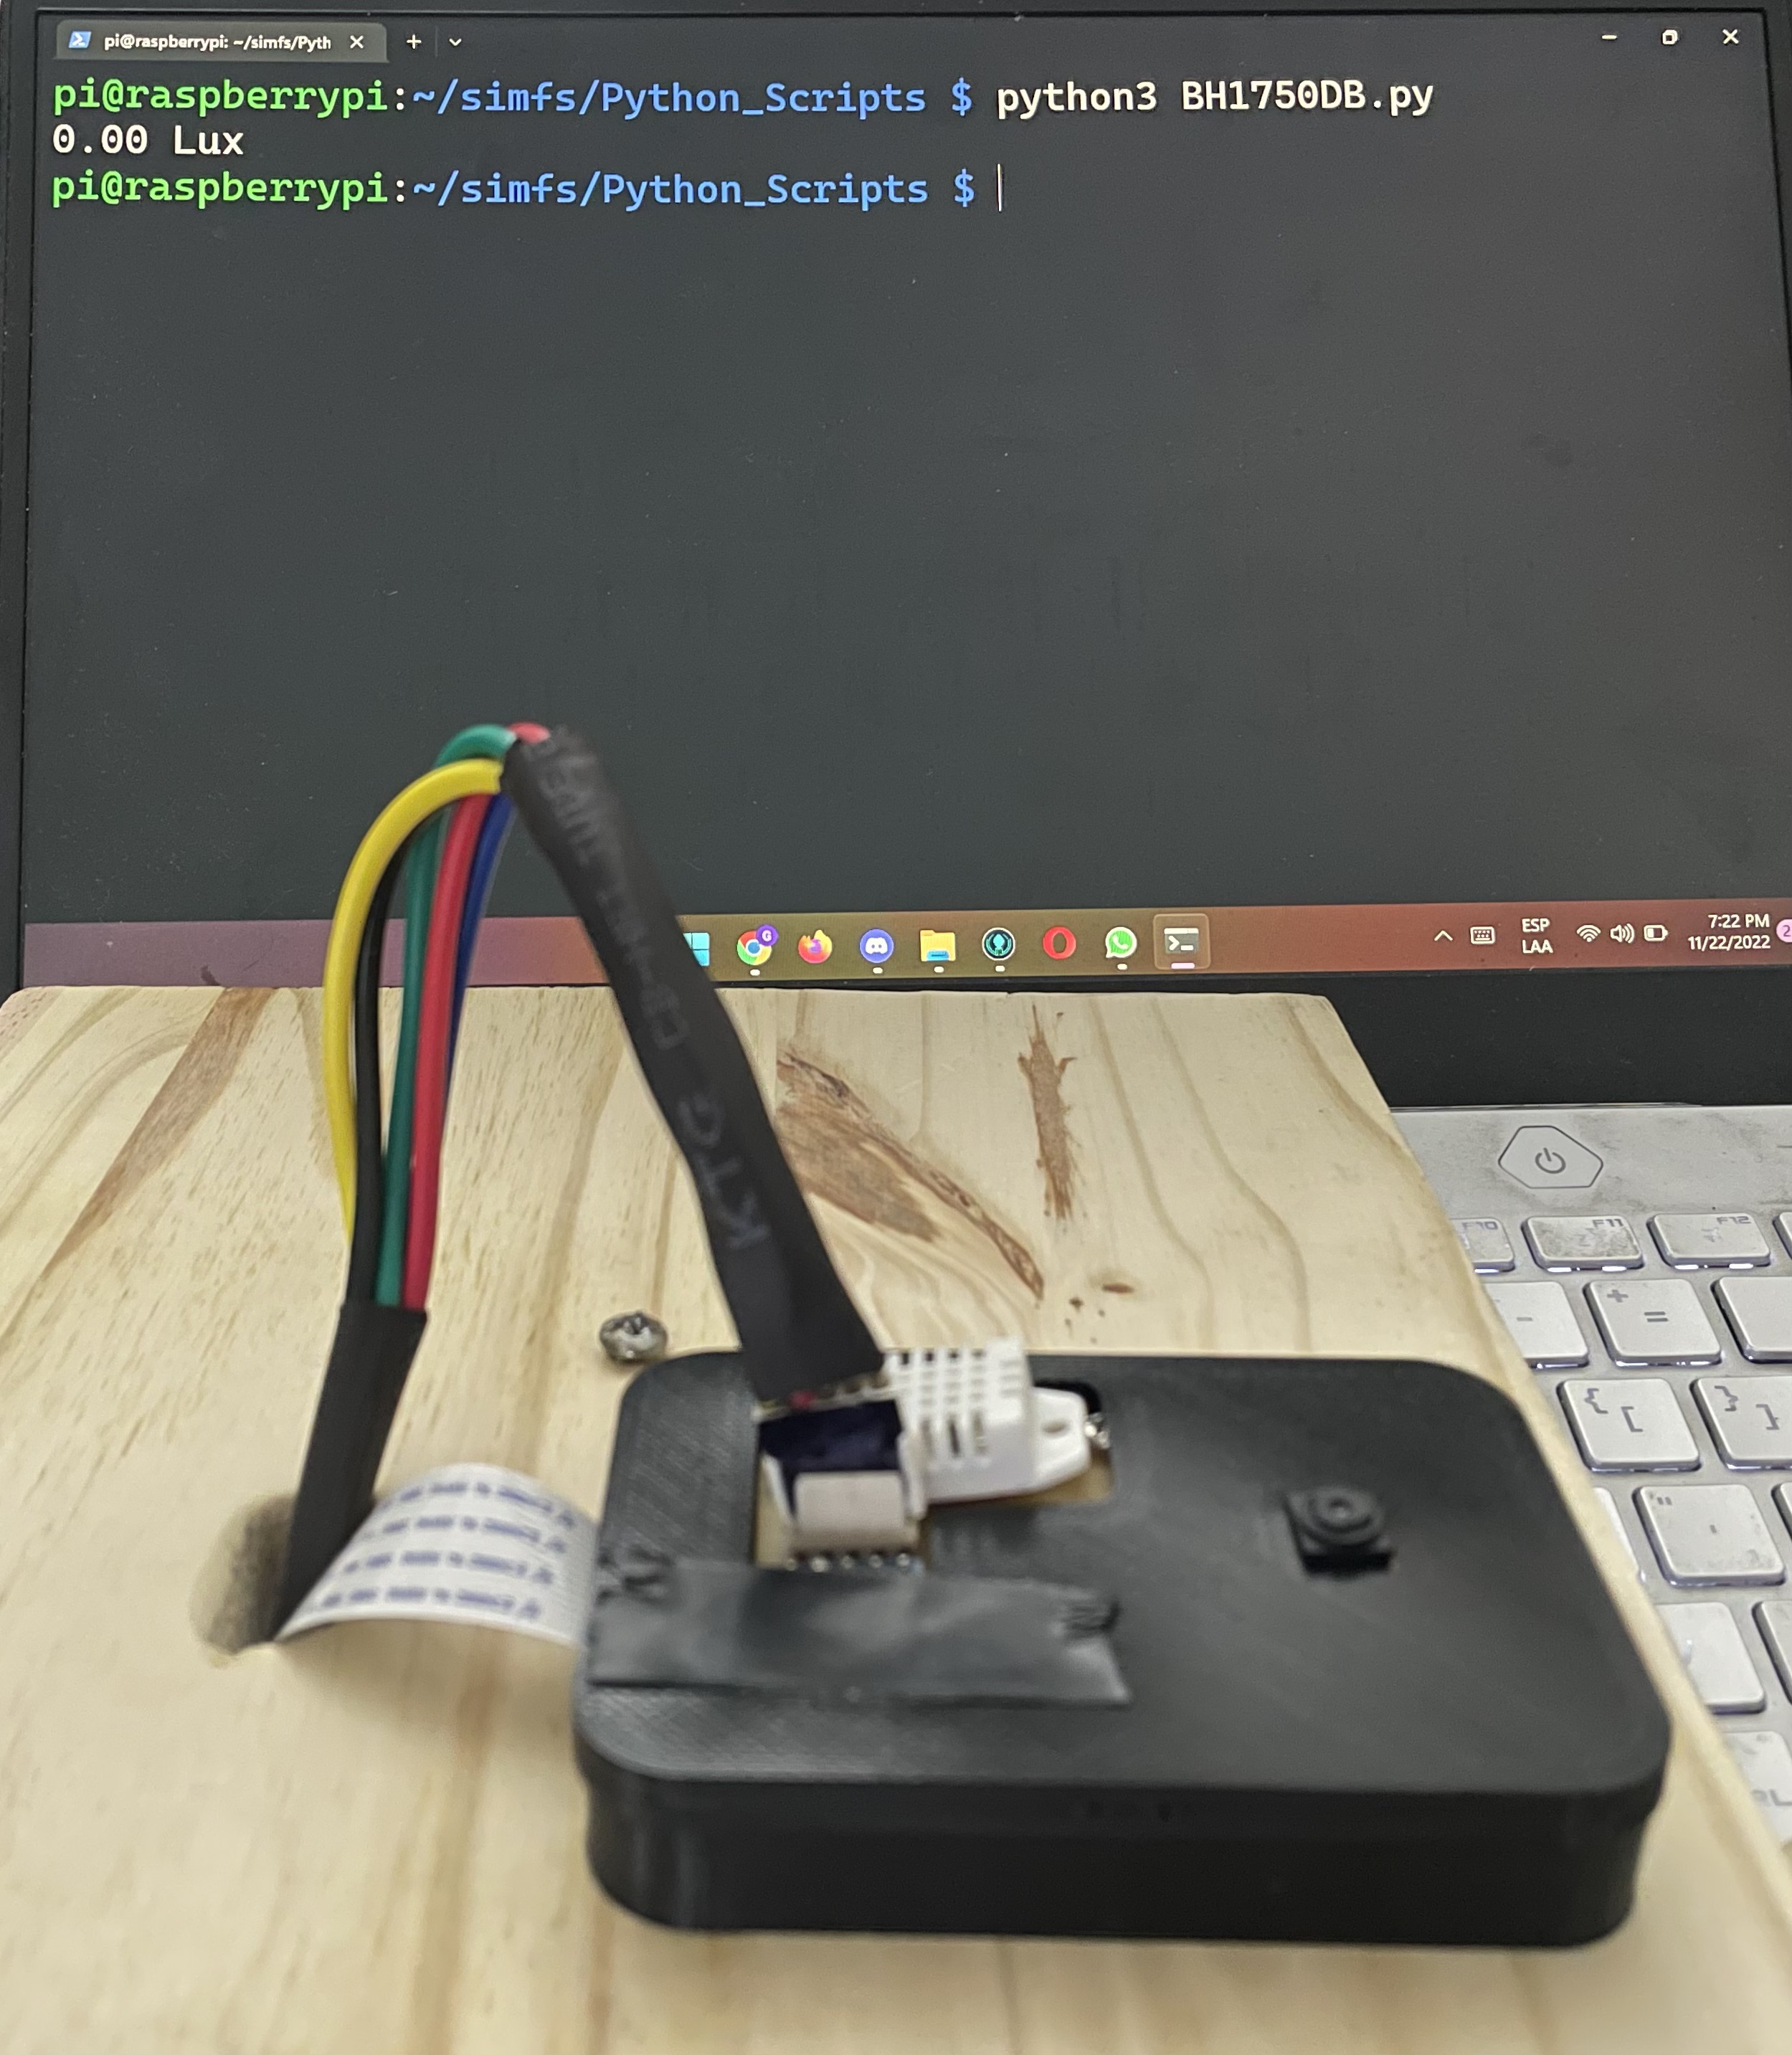
\includegraphics[width=\linewidth]{ImagenesValidacion del prototipo/TINTFUN3a}
        \caption{Sensor cubierto.}
	\end{subfigure}\hfill
    \begin{subfigure}{0.33\textwidth}
    	\centering
        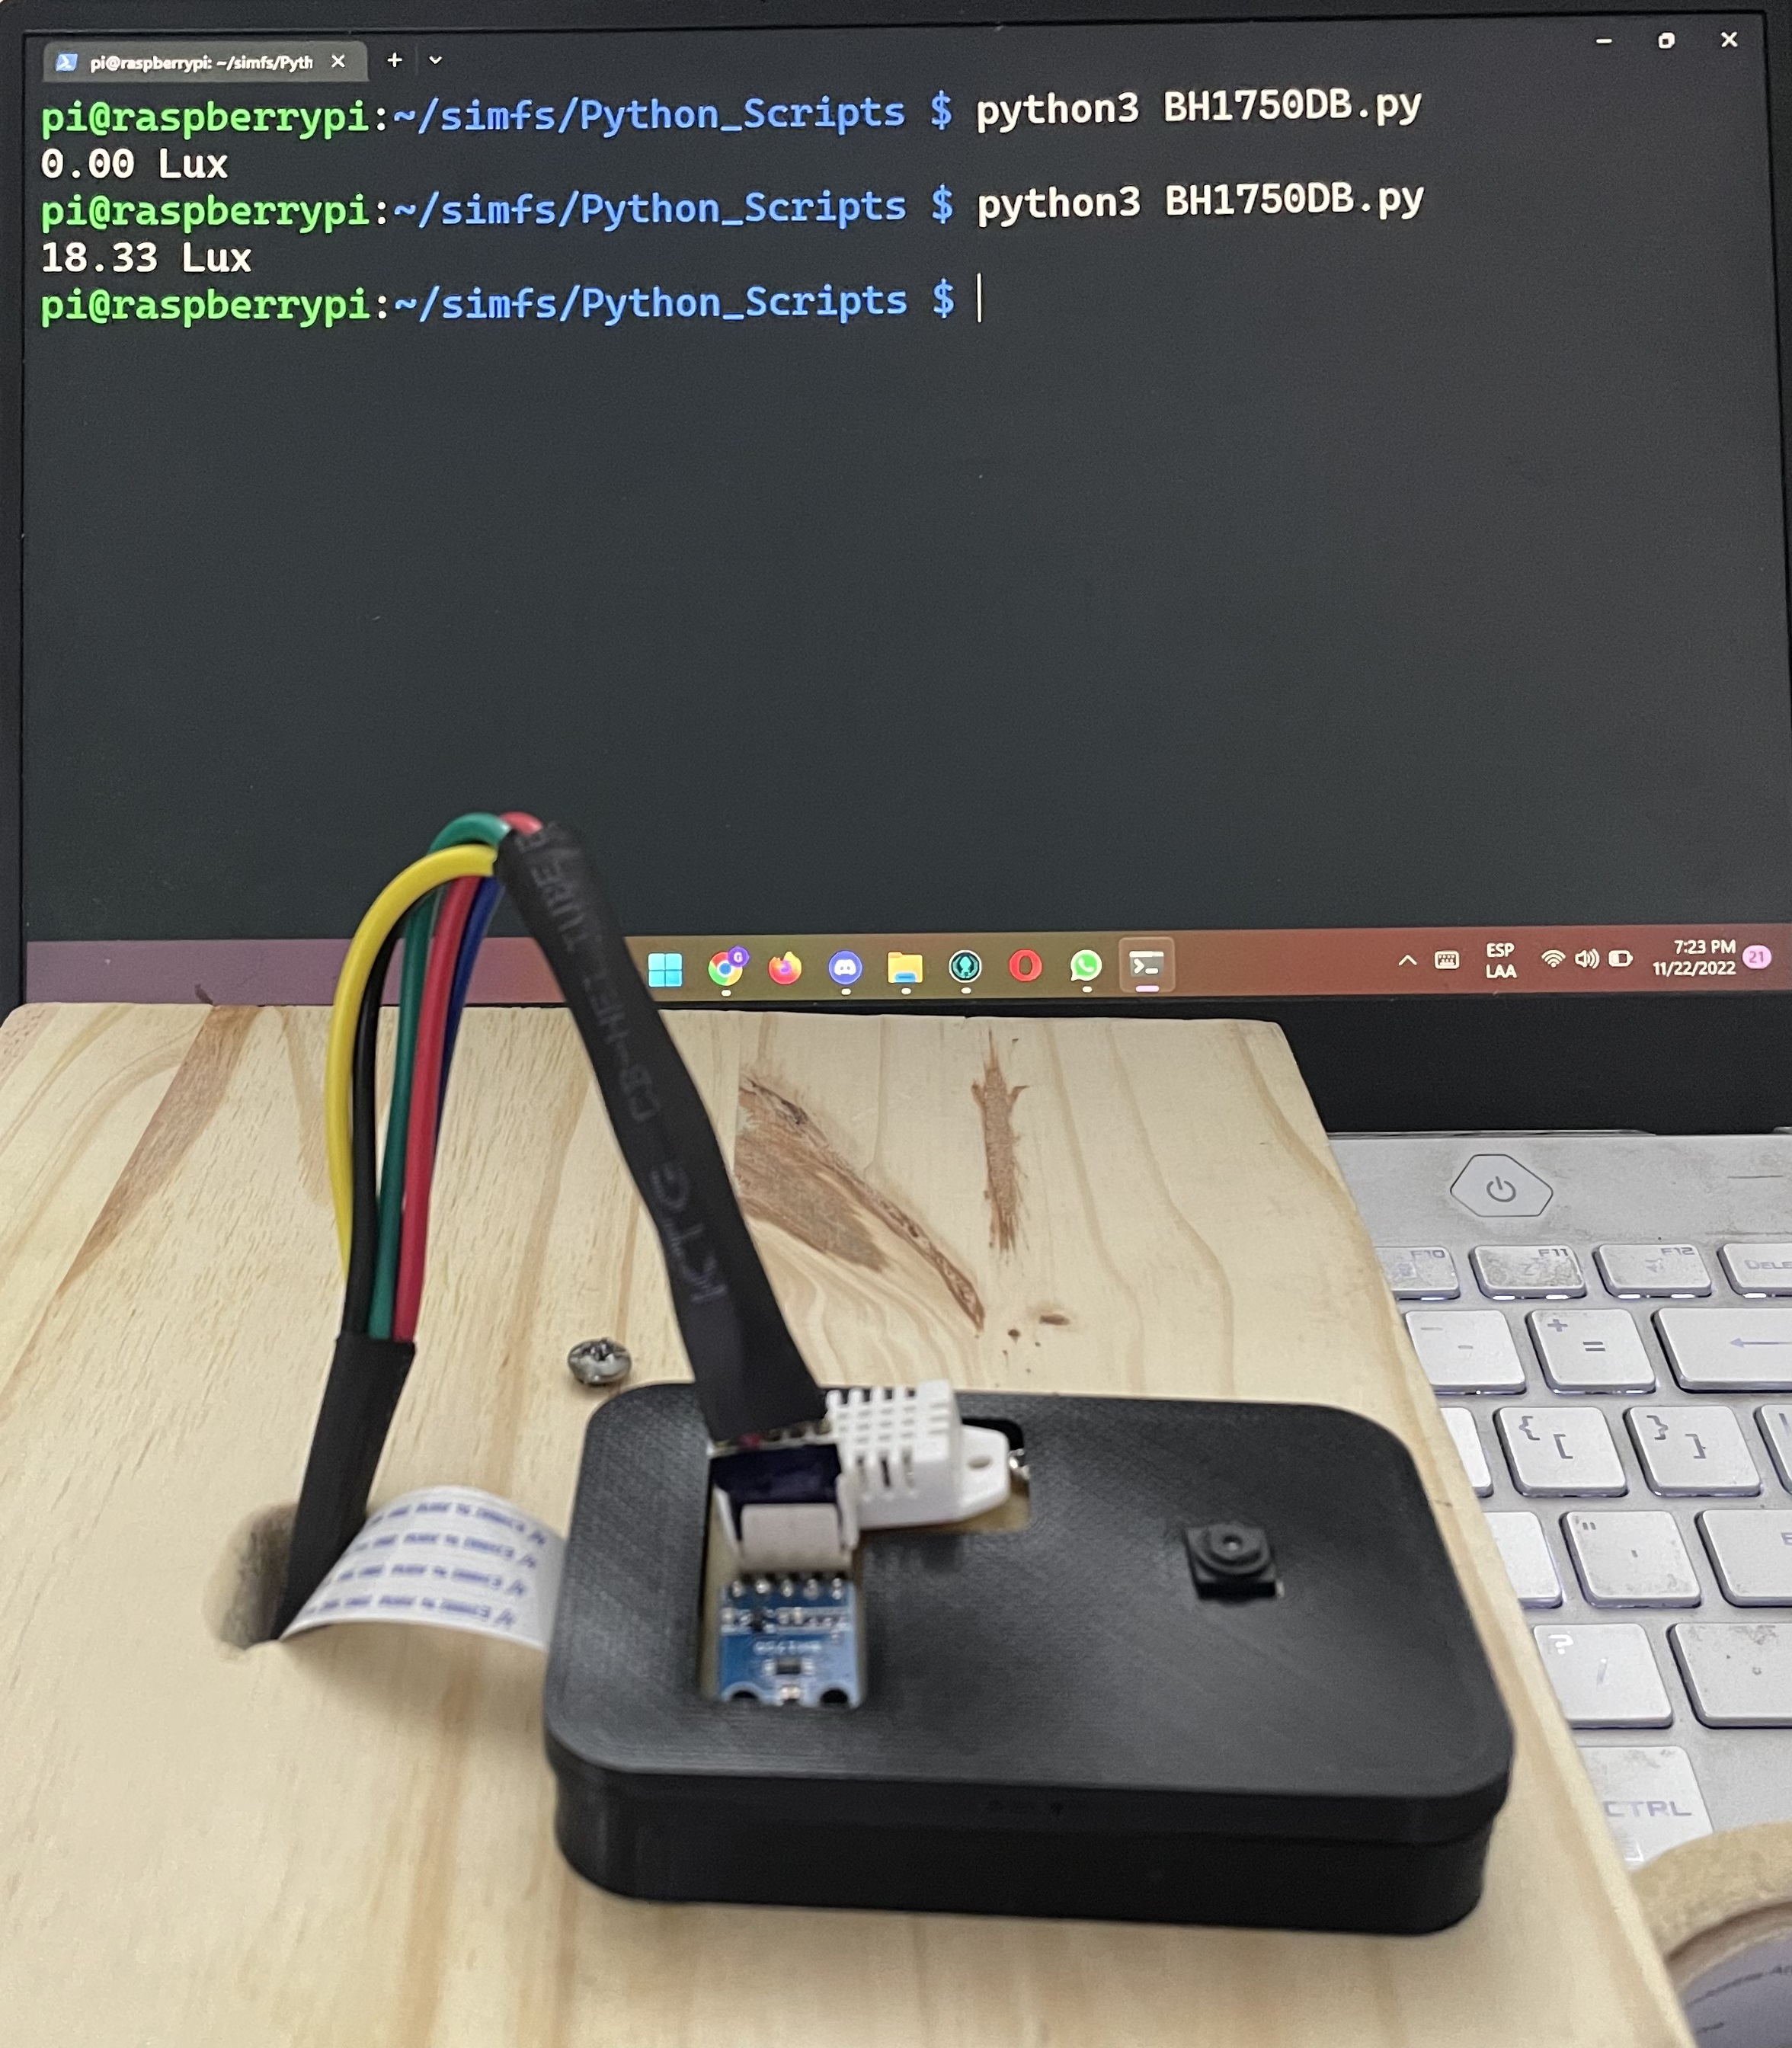
\includegraphics[width=\linewidth]{ImagenesValidacion del prototipo/TINTFUN3b}
        \caption{Sensor descubierto.}
	\end{subfigure}\hfill
    \begin{subfigure}{0.33\textwidth}
    	\centering \vspace*{2.5mm}
        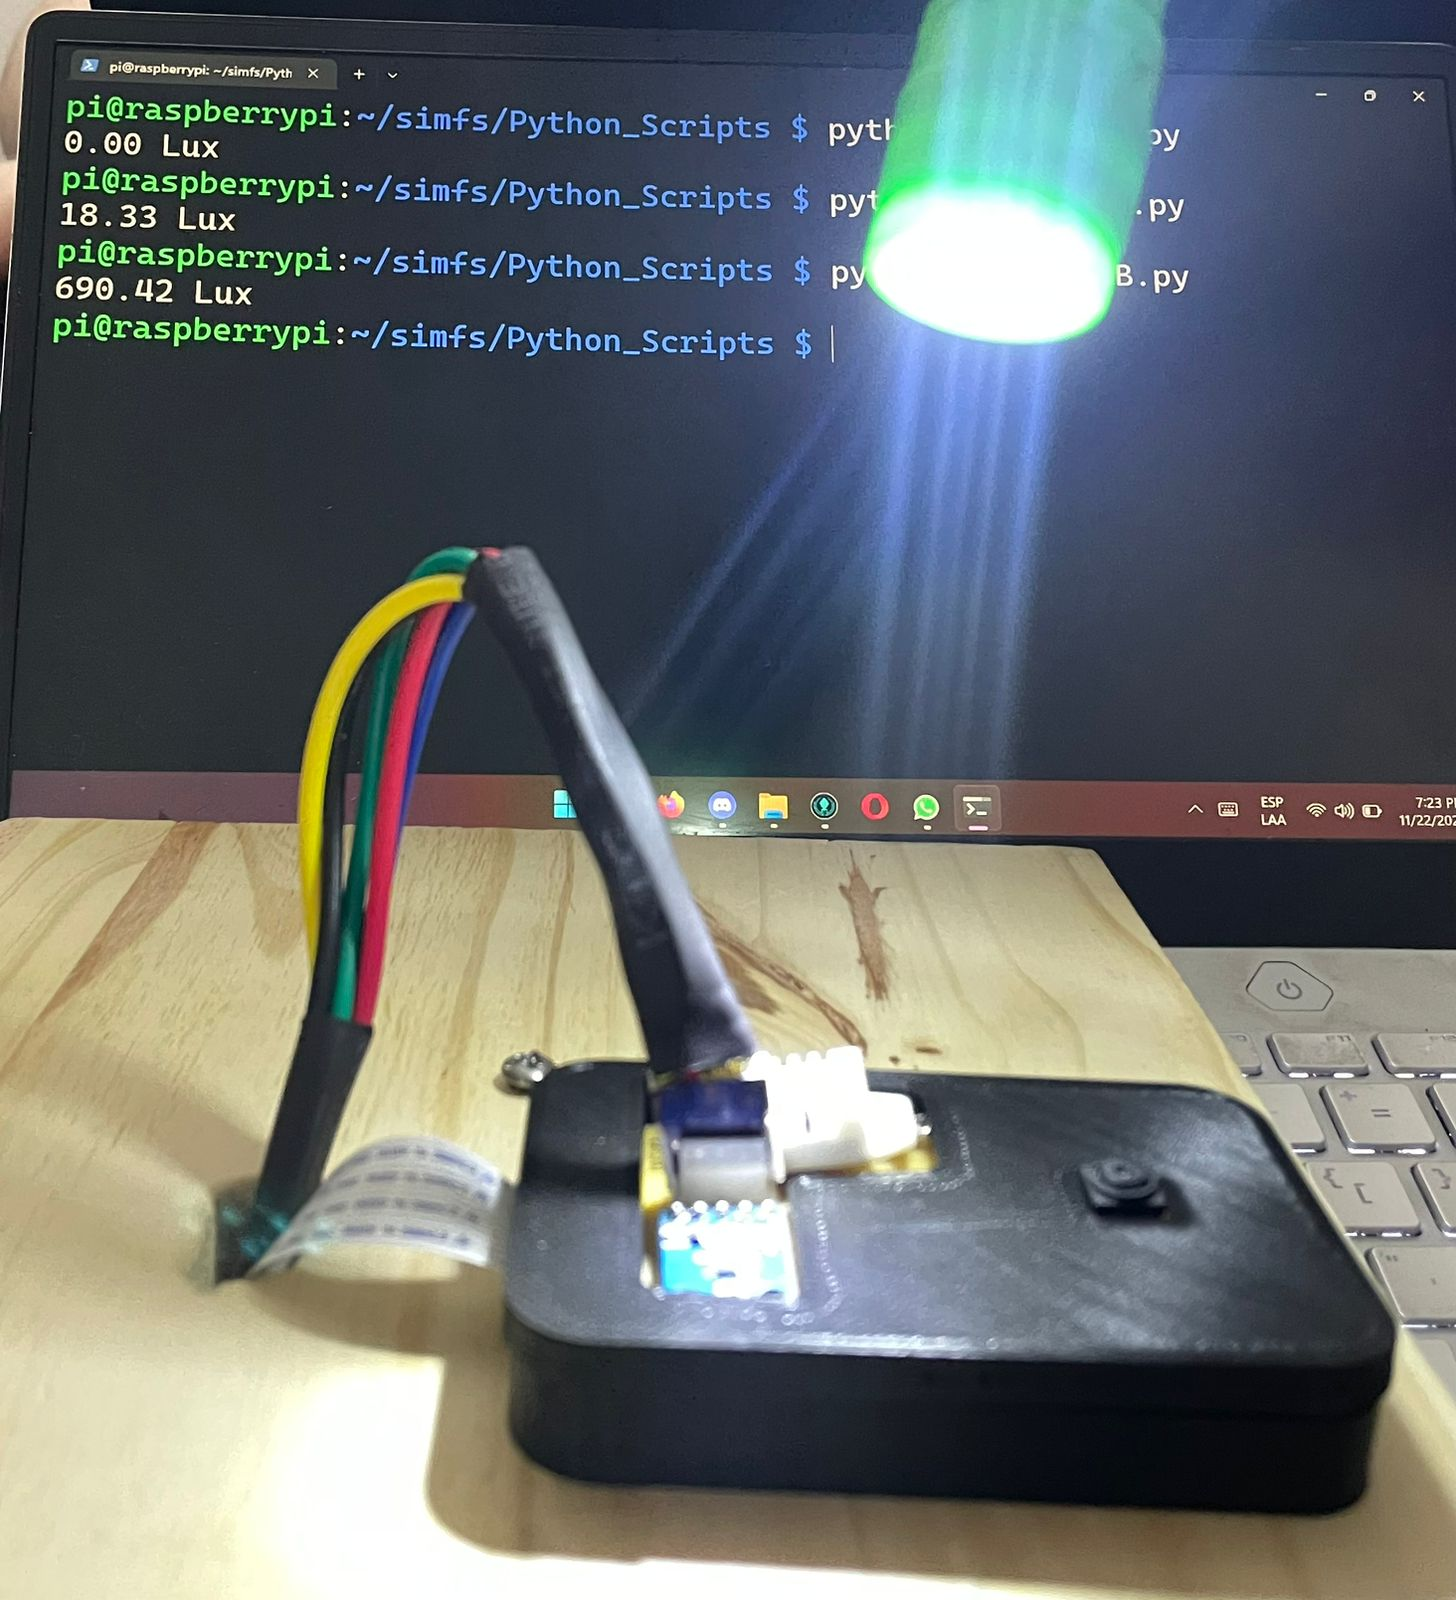
\includegraphics[width=\linewidth]{ImagenesValidacion del prototipo/TINTFUN3c}
        \caption{Sensor descubierto y apuntado con una linterna.}
	\end{subfigure}
	\caption{Validación de seguridad \textit{T-INT-FUN-03}.}
	\label{fig:valLum}
\end{figure}

Disponiendo del banco de pruebas \#3, se corroboró mediante observación los tests de funcionalidad \textit{T-INT-FUN-04} y \textit{T-INT-FUN-12}. Se garantizó que la imagen mostrada al usuario sea la adecuada y que se vea de manera fidedigna, es decir que la transmisión sea de calidad y fluida.
\begin{figure}[H]
	\centering
    	\begin{subfigure}{0.49\textwidth}
        	\centering
        	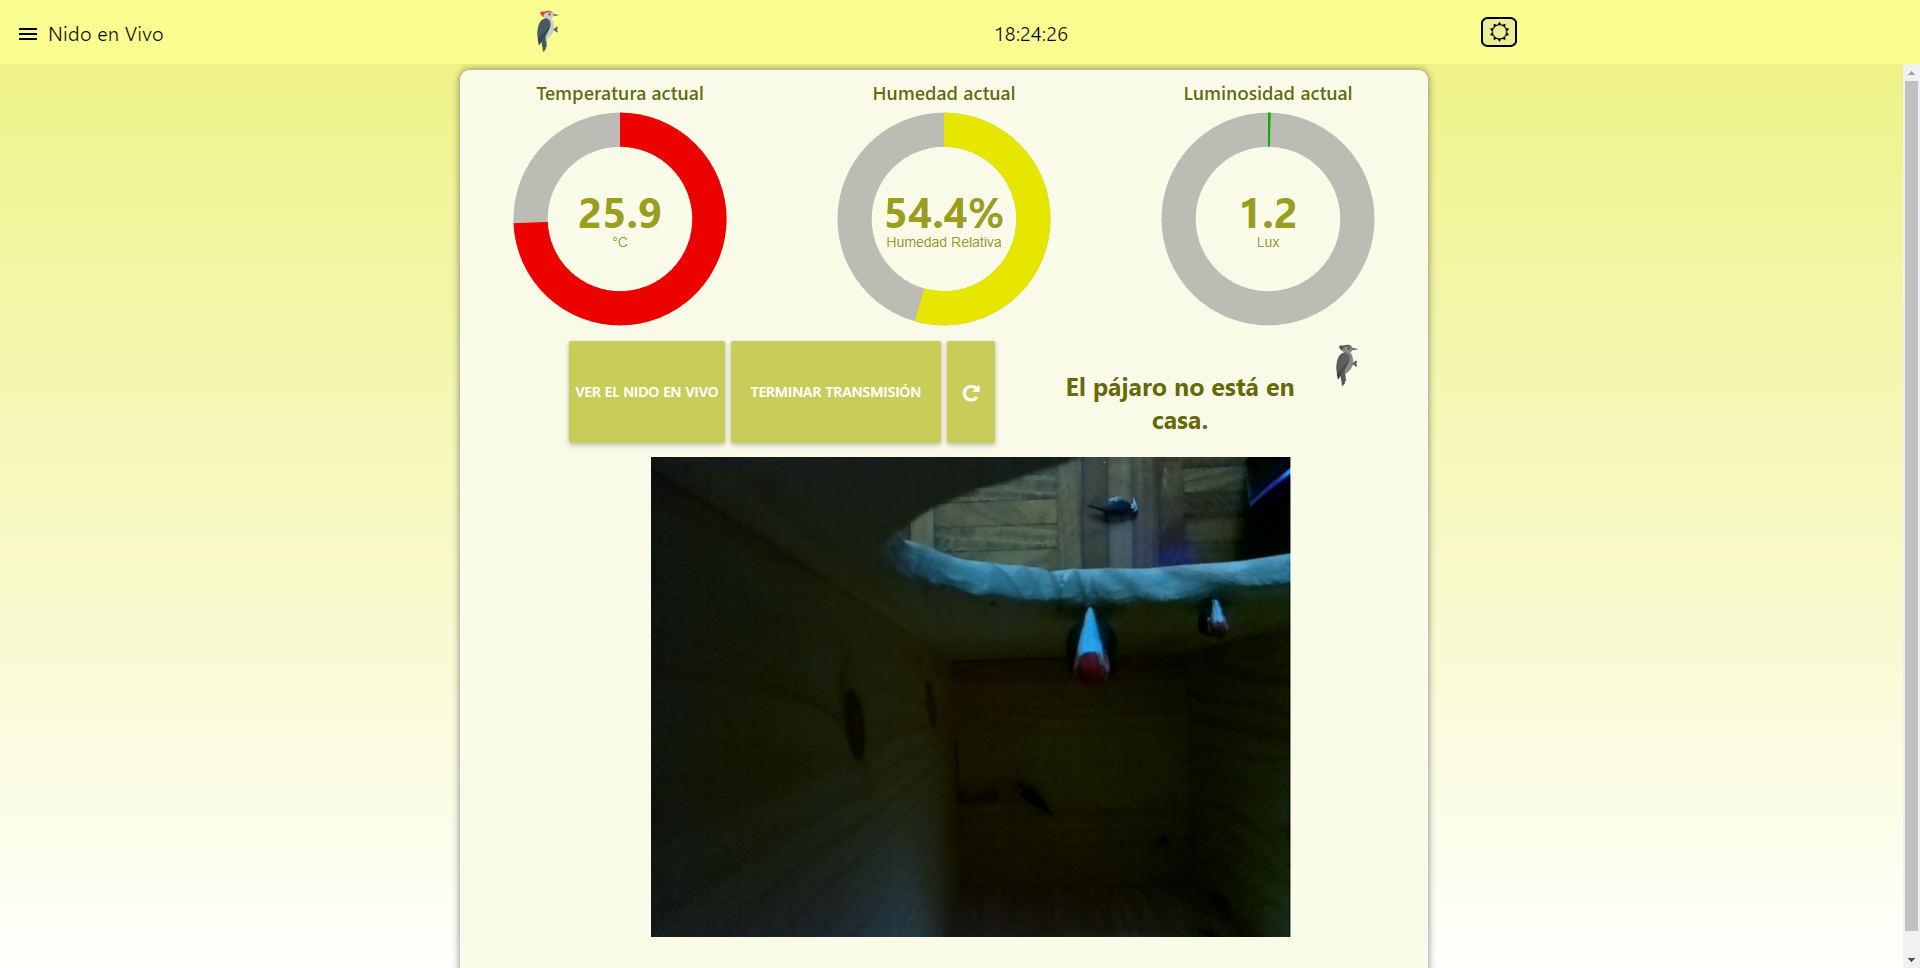
\includegraphics[width=\linewidth]{ImagenesValidacion del prototipo/t-int-fun-04-12-1}		
			\caption{Vista de la transmisión en vivo del nido.}
        \end{subfigure}\hfill
        \begin{subfigure}{0.49\textwidth}
        	\centering        	
        	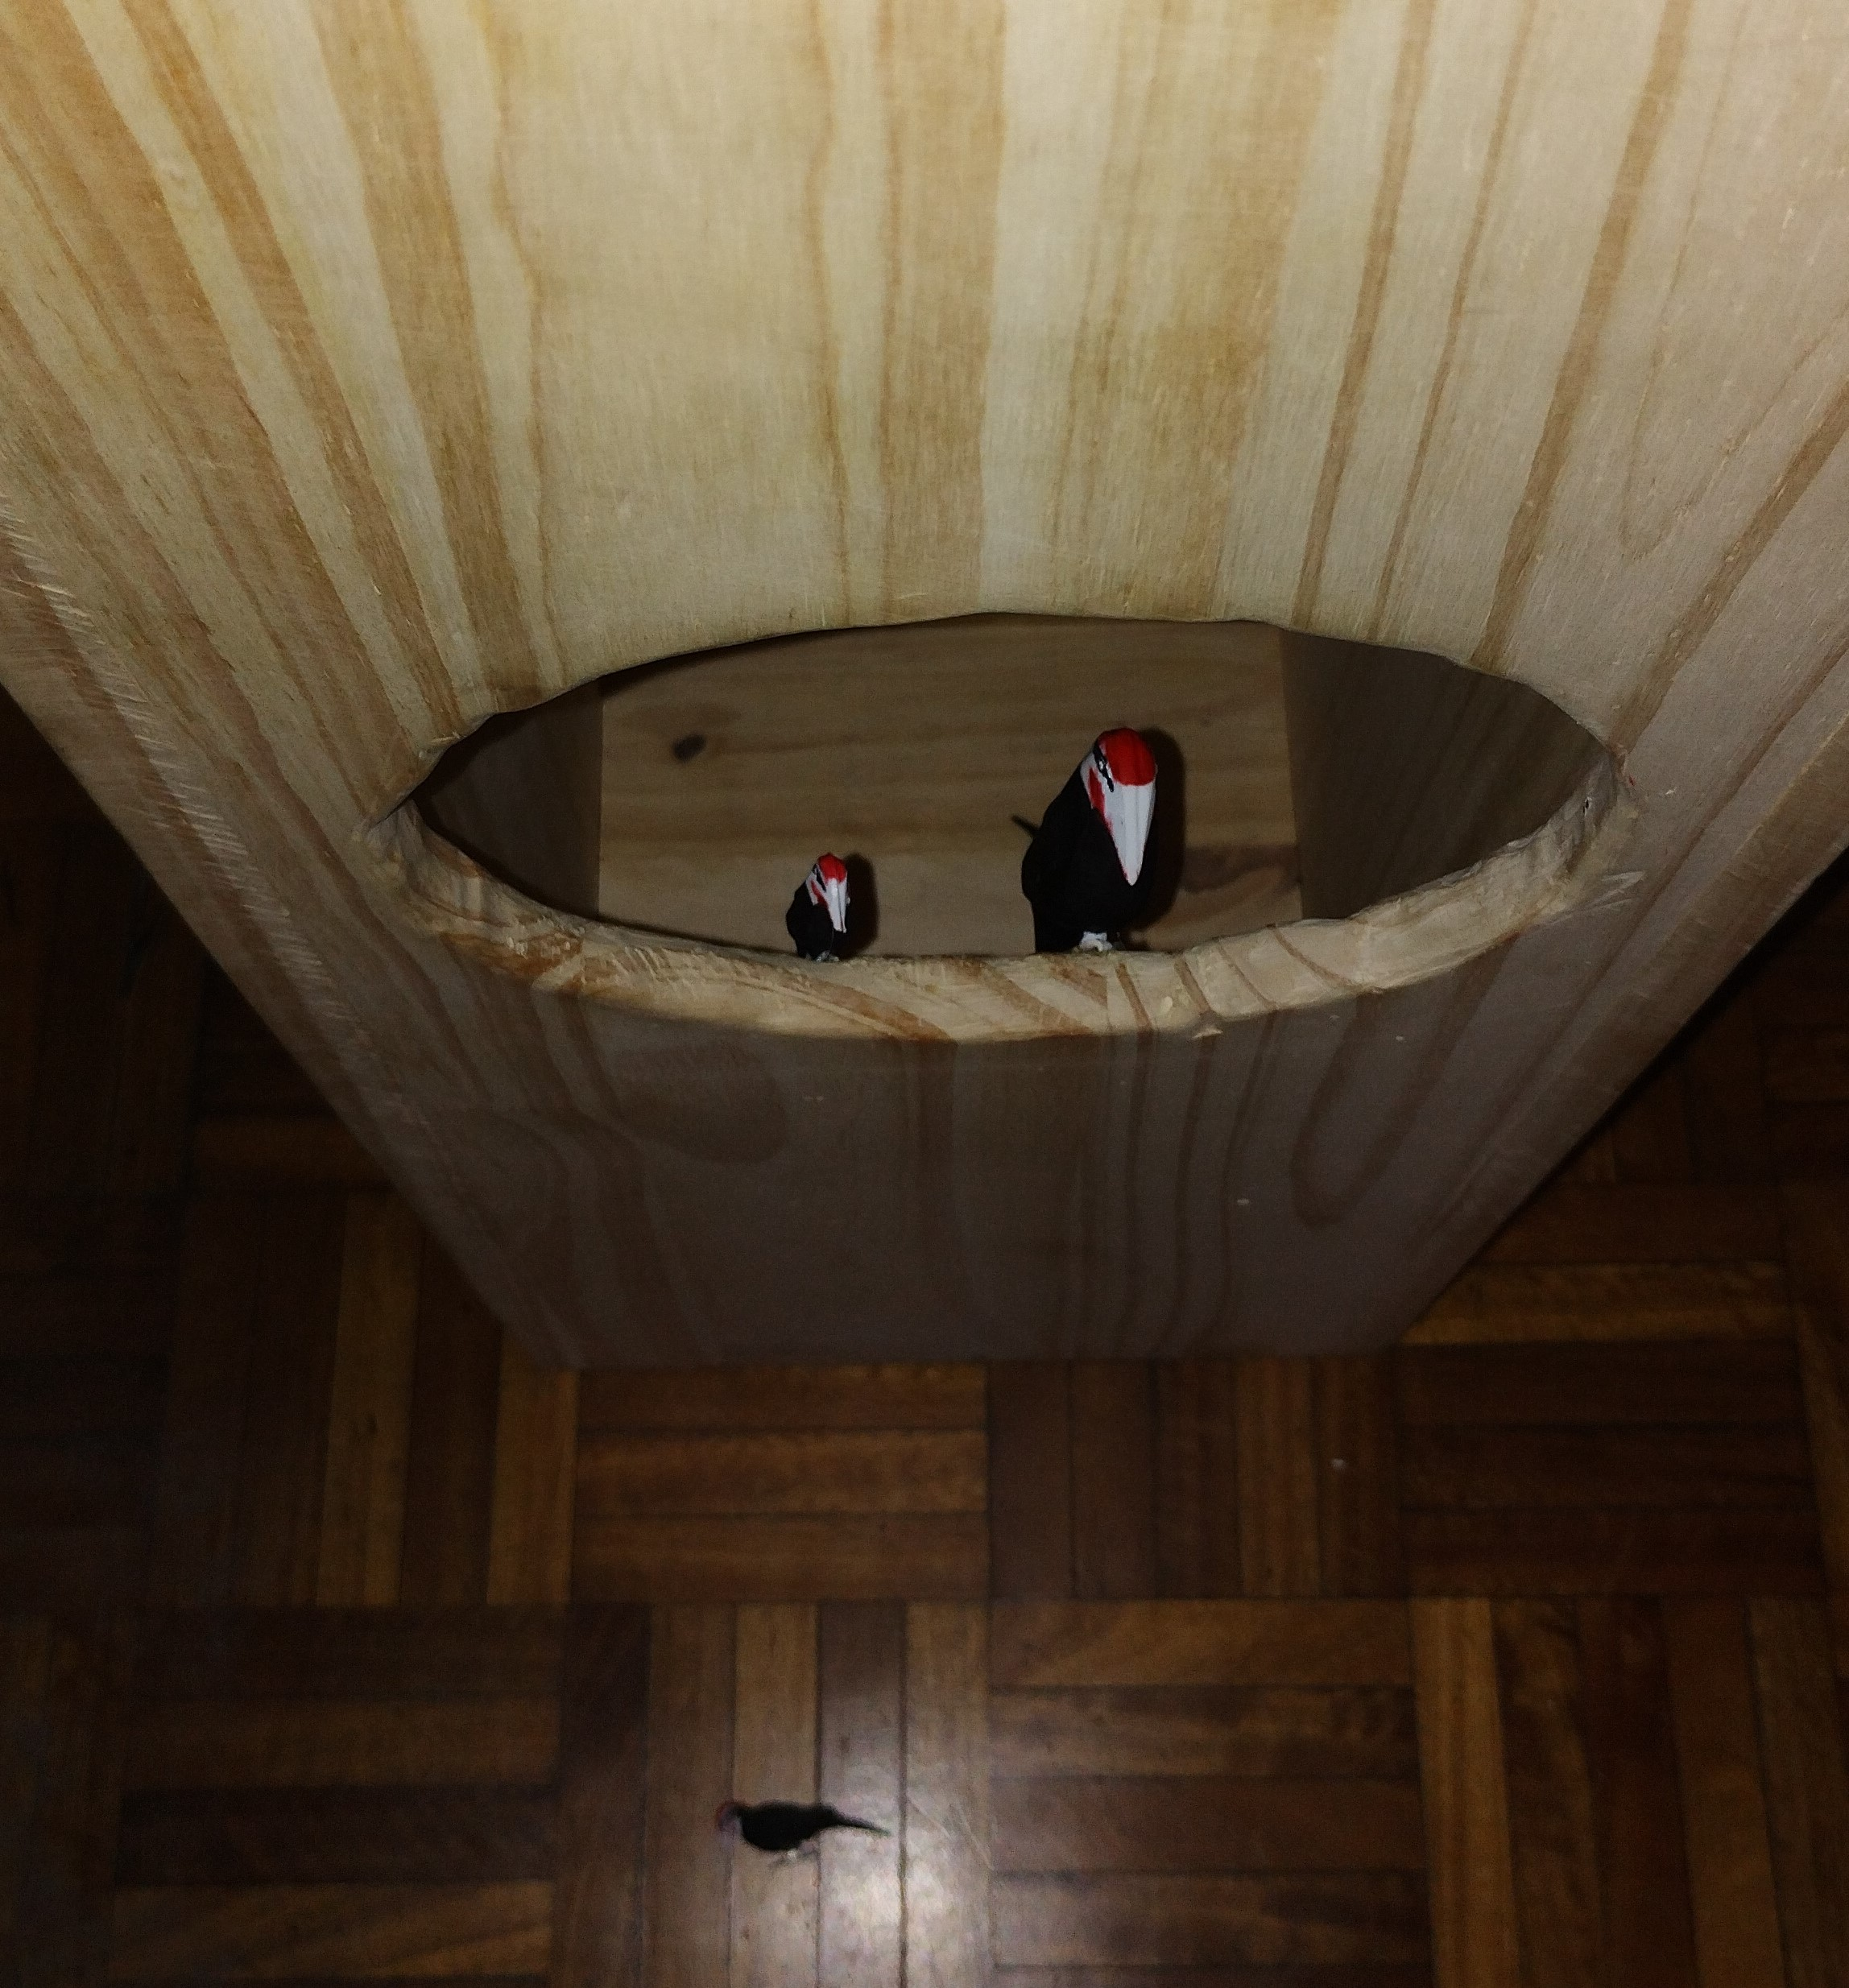
\includegraphics[width=0.5\linewidth]{ImagenesValidacion del prototipo/t-int-fun-04-12-2}
        	\caption{Imagen del exterior del nido en el momento de la trasmisión.}
        \end{subfigure}
	\caption{Validación de funcionalidad \textit{T-INT-FUN-04} y \textit{T-INT-FUN-12}.}
\end{figure}

El test de \textit{T-INT-FUN-05} se concluyó de manera satisfactoria. Resultados similares a los obtenidos se encuentran presentes en la Figura (\ref{fig:foto_camara_filtro}), donde se comparan fotos similares con y sin filtro. Por otro lado, se realiza la prueba \textit{T-INT-FUN-06}, donde se varió la posición del módulo BLE, observando los cambios de su presencia.
\begin{figure}[H]
	\centering
		\begin{subfigure}{0.49\textwidth}
			\centering
			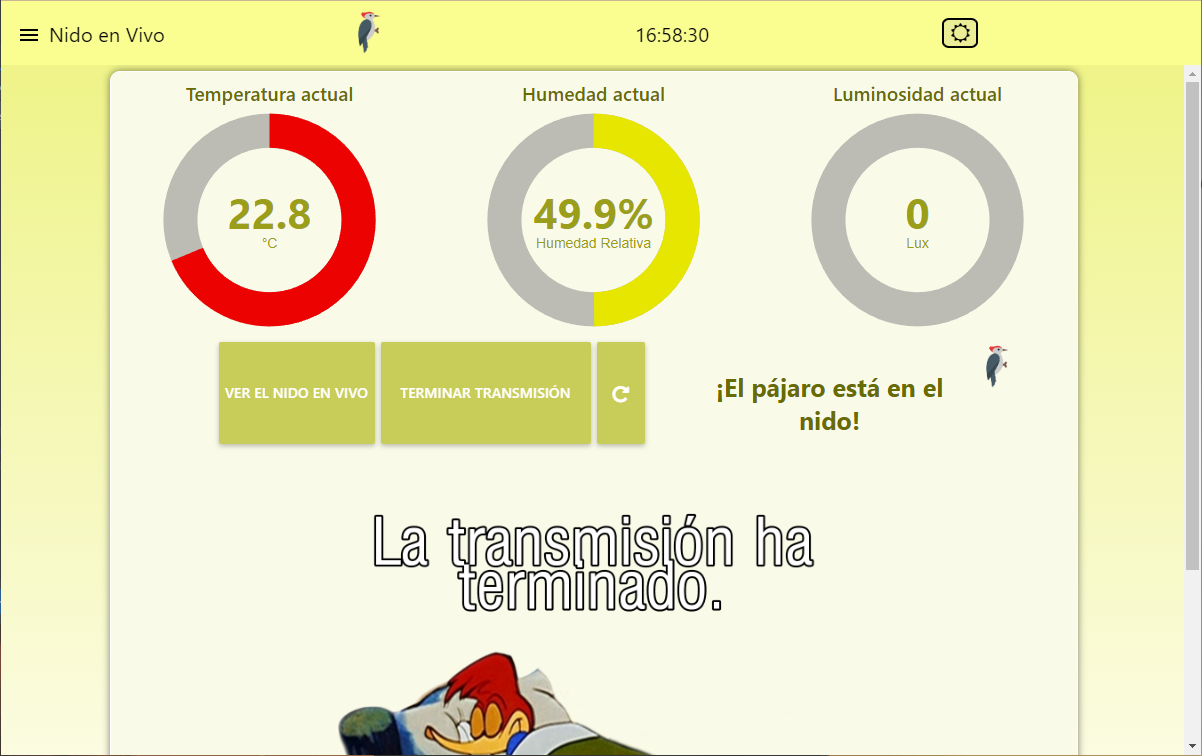
\includegraphics[width=\linewidth]{ImagenesValidacion del prototipo/T-INT-FUN-6-1}		
			\caption{\quotes{El pájaro está en el nido}.}
		\end{subfigure}\hfill
		\begin{subfigure}{0.49\textwidth}
			\centering
			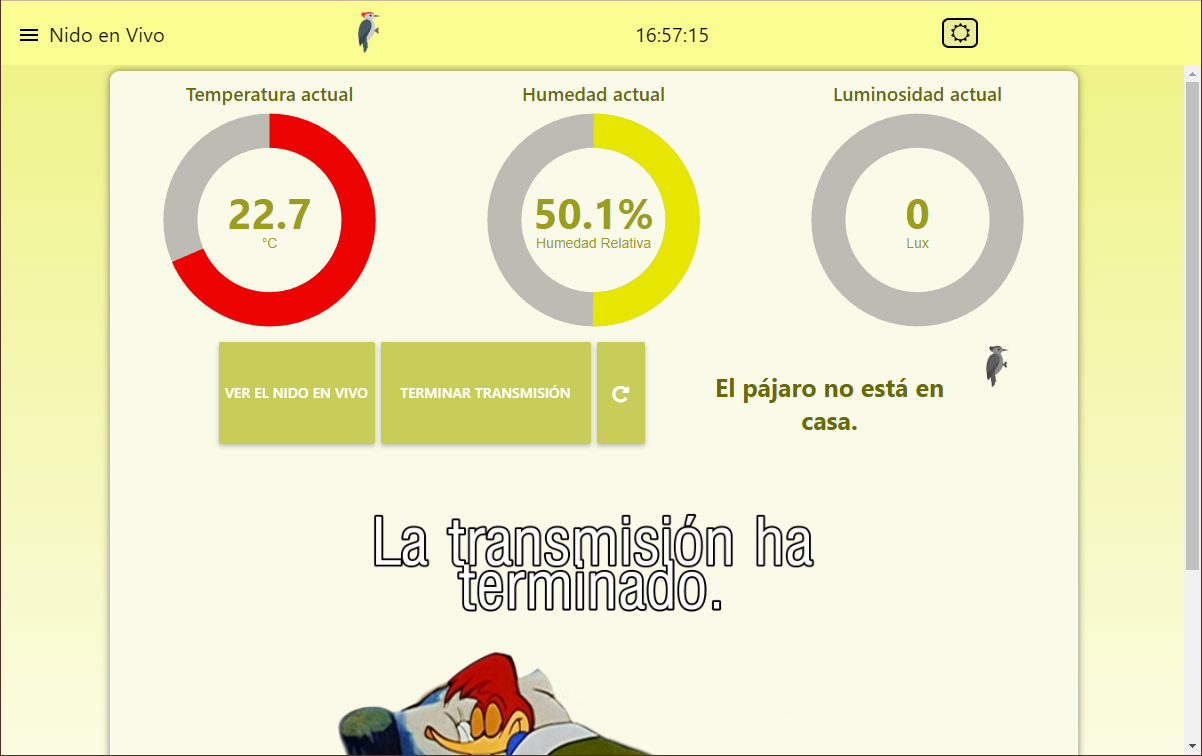
\includegraphics[width=\linewidth]{ImagenesValidacion del prototipo/T-INT-FUN-6-2}
			\caption{\quotes{El pájaro no está en casa}.}
		\end{subfigure}		
		
		\begin{subfigure}{0.49\textwidth}
			\centering
			\includegraphics[width=\linewidth]{ImagenesValidacion del prototipo/T-INT-FUN11a}	
			\caption{Beacon fuera del nido.}
		\end{subfigure}\hfill
		\begin{subfigure}{0.49\textwidth}
			\centering
			\includegraphics[width=\linewidth]{ImagenesValidacion del prototipo/T-INT-FUN11b}
		\caption{Beacon en el nido.}
		\end{subfigure}
	\caption{Variación de posición del beacon con respecto al nido.}
\end{figure}

Las validaciones a continuación están relacionadas con aspectos funcionales de los sensores. Se comienza con el periodo de muestreo de estos como indica \textit{T-INT-FUN-07}. Se puede corroborar que las mediciones son cada 5 minutos.
\begin{figure}[H]
	\centering
    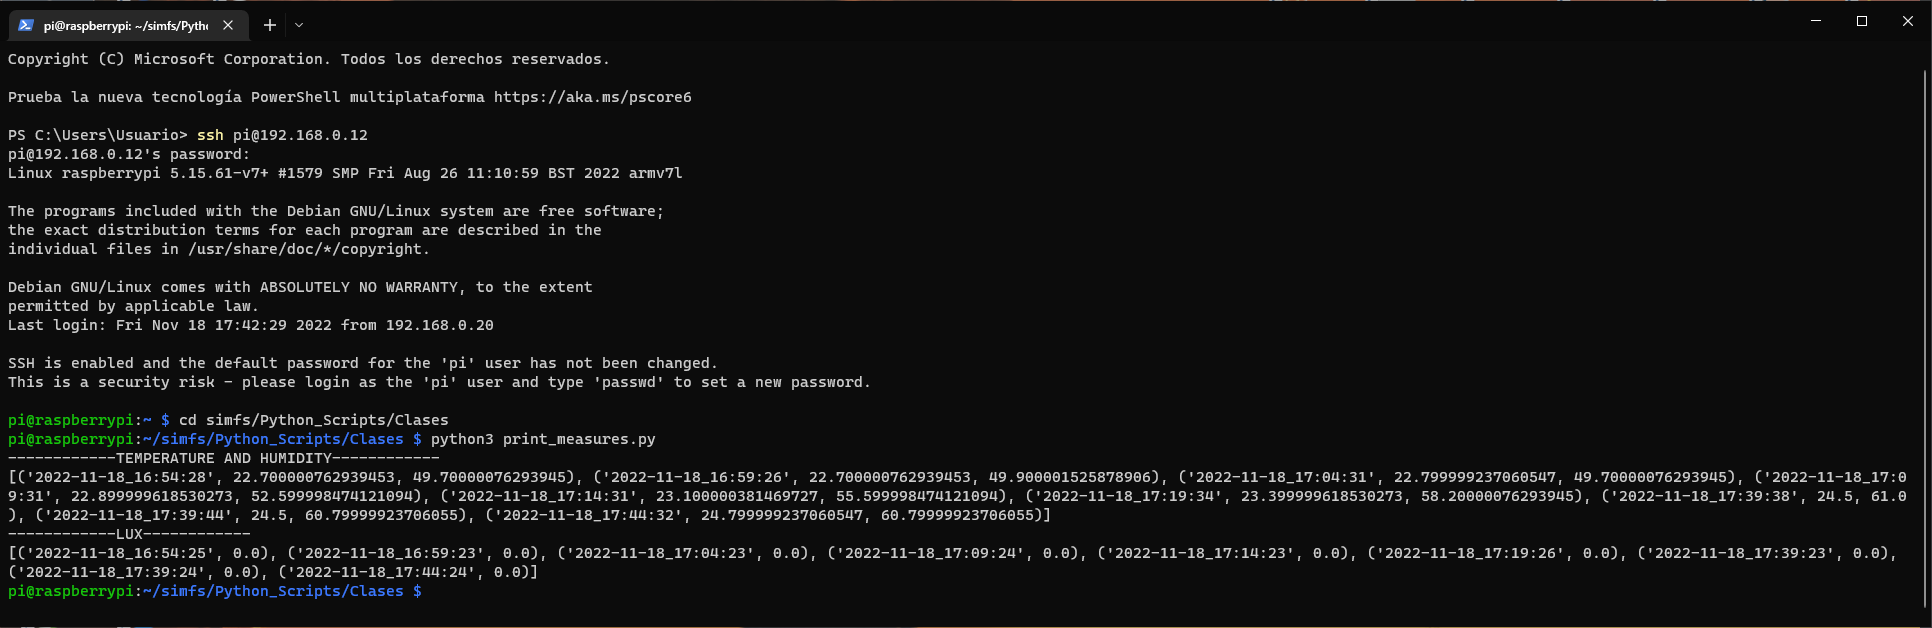
\includegraphics[width=\linewidth]{ImagenesValidacion del prototipo/T-INT-FUN-07}
	\caption{Validación de funcionalidad \textit{T-INT-FUN-07}.}
\end{figure}

Para \textit{T-INT-FUN-08} se observa que el tiempo obtenido en consola como el de la computadora, presentado en la parte inferior derecha de la imagen, coinciden. Es por esto que se considera que la prueba concluyó de manera exitosa.
\begin{figure}[H]
	\centering
    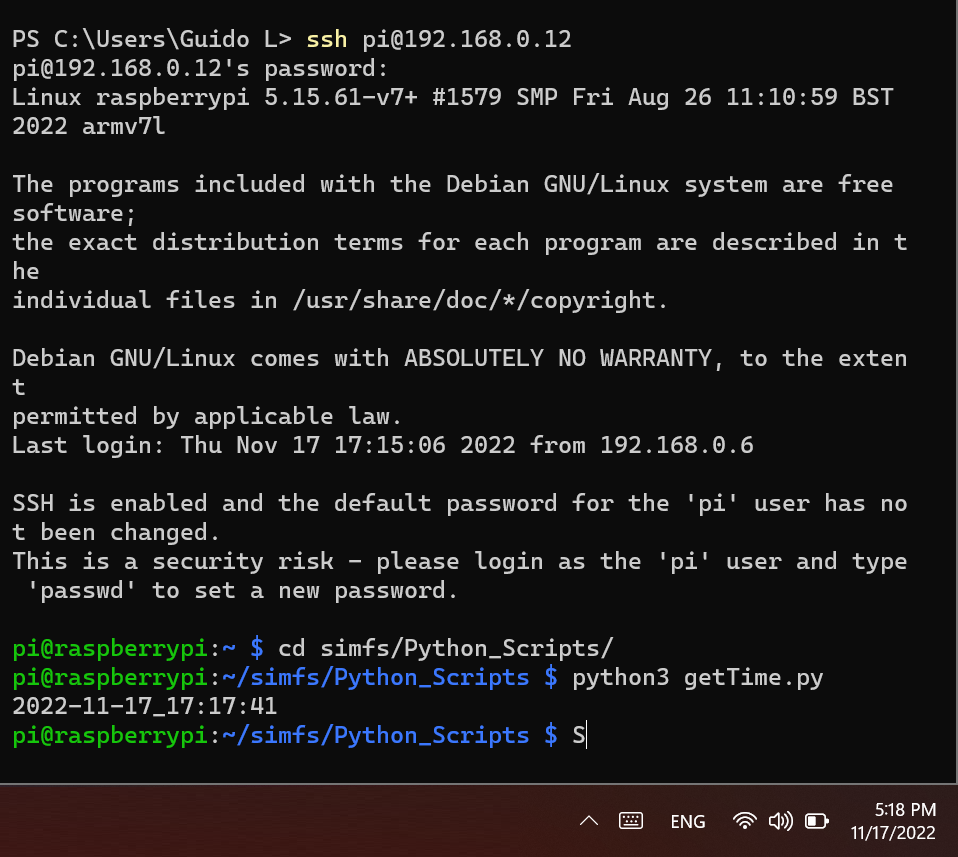
\includegraphics[width=0.8\linewidth]{ImagenesValidacion del prototipo/TINTFUN8}
	\caption{Validación de funcionalidad \textit{T-INT-FUN-08}.}
\end{figure}

La siguiente prueba corresponde a \textit{T-INT-FUN-09}. En esta se desenergiza la \rspi, y luego de esperar el tiempo apropiado, se la energiza nuevamente corroborando que la hora correspondiente al módulo RTC sea correcta.
\begin{figure}[H]
	\centering
	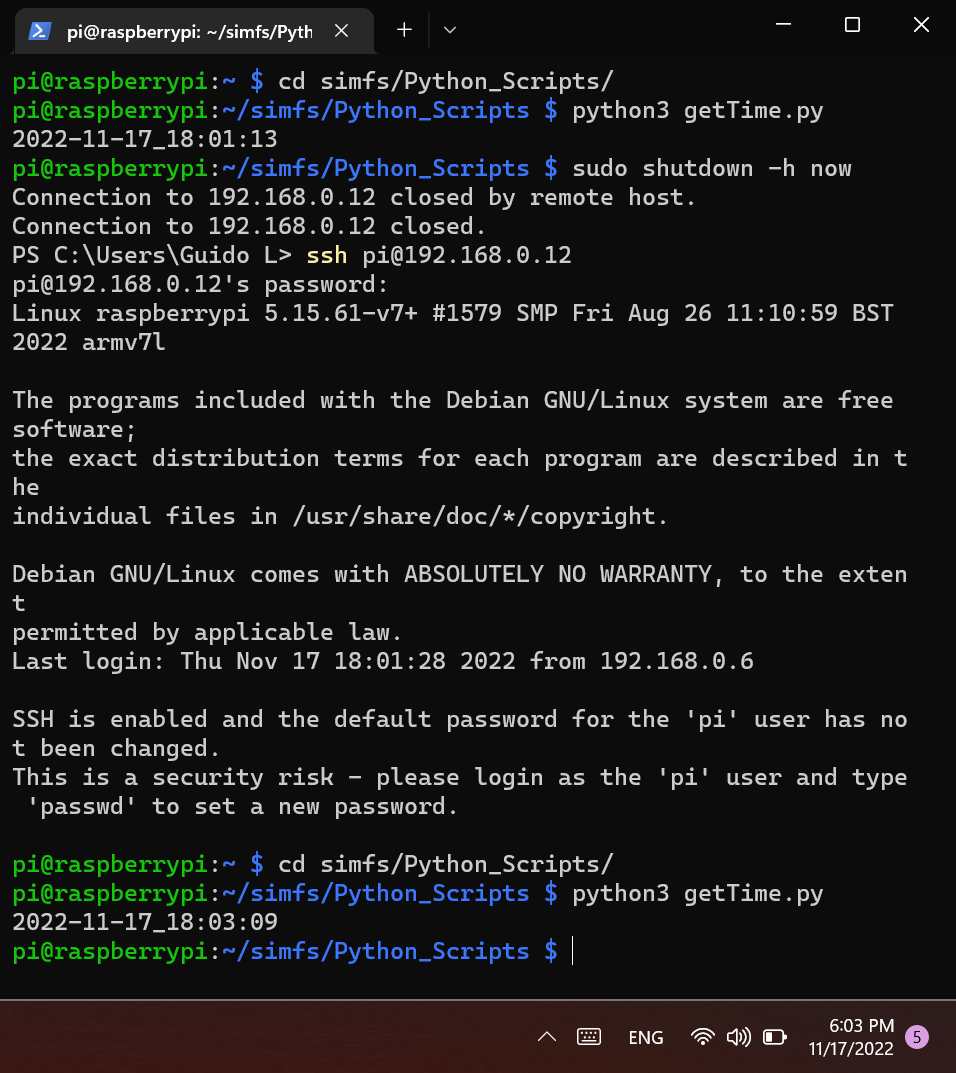
\includegraphics[width=0.8\linewidth]{ImagenesValidacion del prototipo/TINTFUN9}
	\caption{Validación de funcionalidad \textit{T-INT-FUN-09}.}
\end{figure}

\Subsection{Validación Pruebas de Comunicación 1}
\textit{T-INT-COM1-01} se efectúa disponiendo del banco de pruebas número \#3. Se emplea un dispositivo de comunicación mediante protocolo BLE. Es posible determinar que la transmisión se efectuó ya que se encuentra el archivo de interés entre los datos almacenados de la \rpi.
\begin{figure}[H]
	\centering
	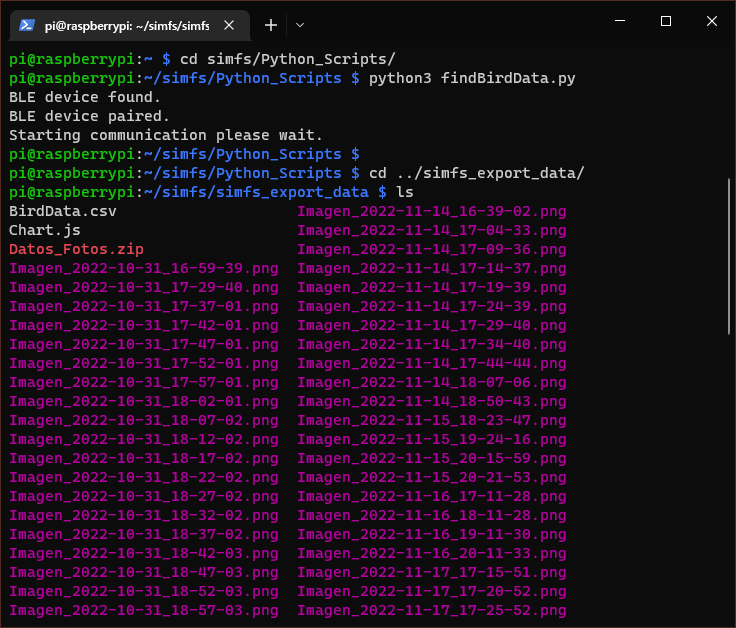
\includegraphics[width=0.8\linewidth]{ImagenesValidacion del prototipo/BirdData2}
	\caption{El archivo \quotes{BirdData.csv} se encuentra entre los archivos disponibles de descarga.}
\end{figure}

De esta forma es posible acceder a esta información mediante la interfaz gráfica del usuario. Se procede descargándolos y comparándolos con los transmitidos. Se observa que la transmisión de datos se realiza sin perdida de paquetes ni resultando con archivos corruptos.
\begin{figure}[H]
	\centering
	\begin{subfigure}{0.49\textwidth}
		\centering
		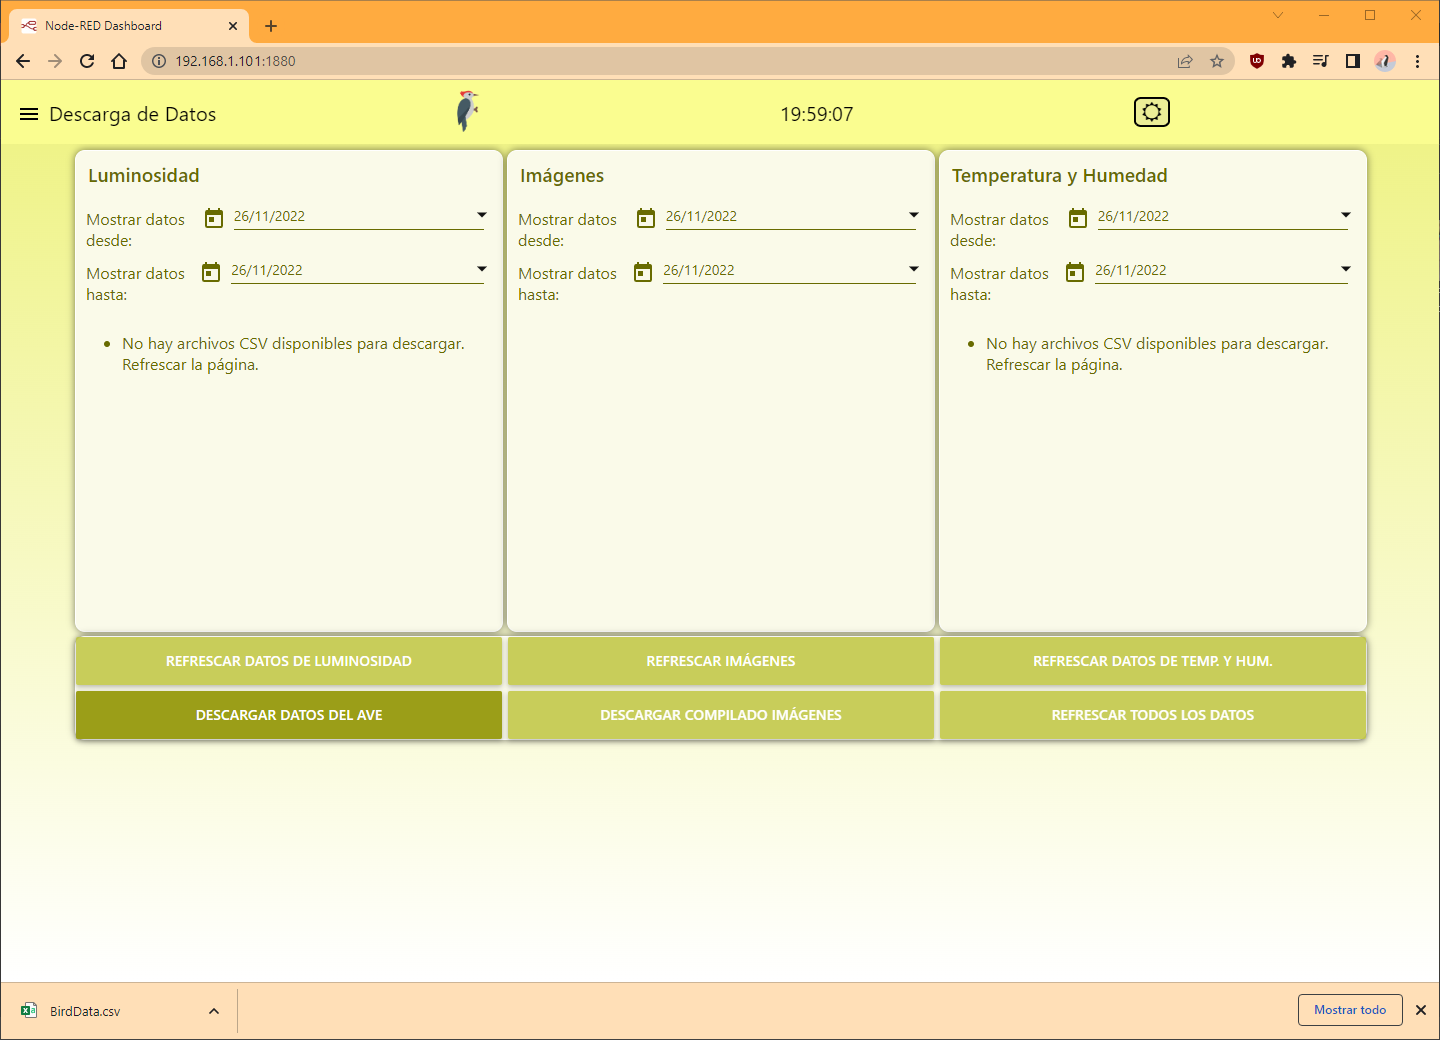
\includegraphics[width=\linewidth]{ImagenesValidacion del prototipo/Descarga-1}		
		\caption{Descarga del archivo en la interfaz gráfica.}
	\end{subfigure}\hfill
	\begin{subfigure}{0.49\textwidth}
		\centering
		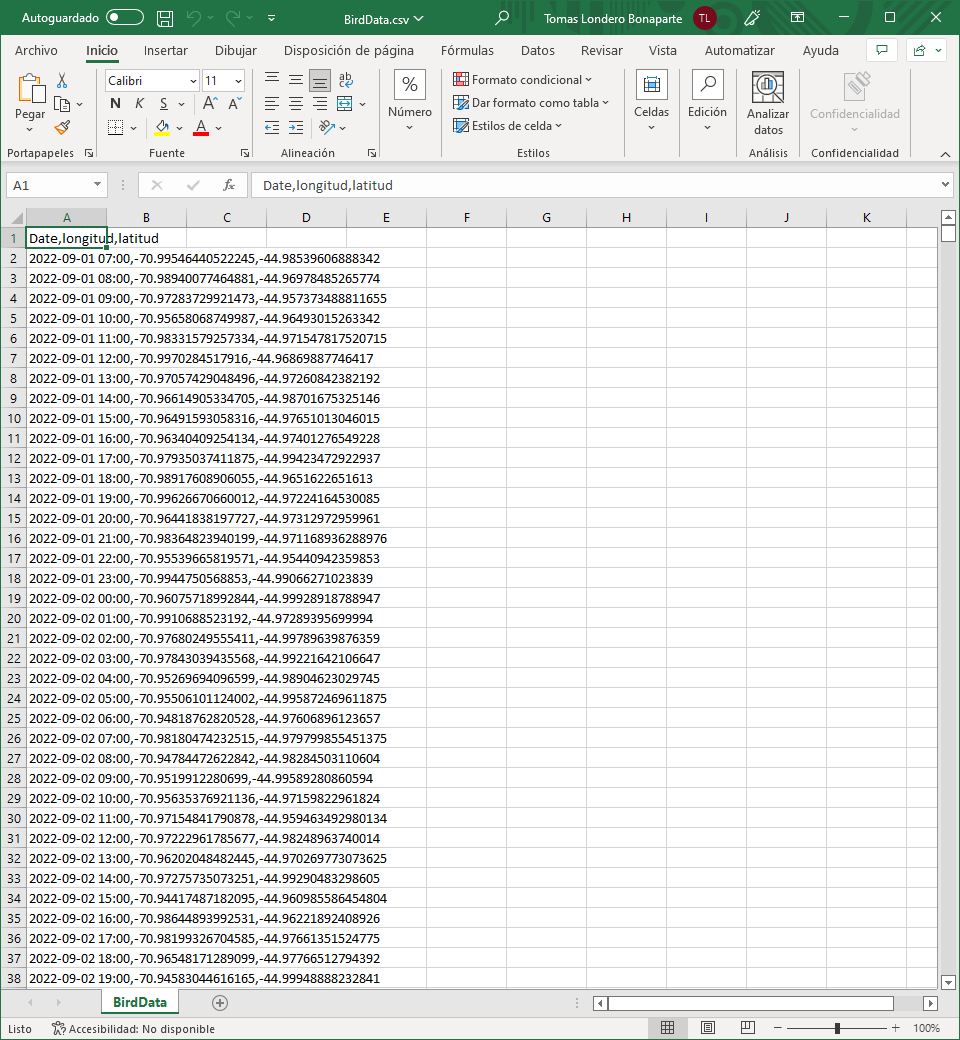
\includegraphics[width=\linewidth]{ImagenesValidacion del prototipo/Descarga-2}
		\caption{Archivo descargado exitosamente.}
	\end{subfigure}
	\caption{Validación \textit{T-COM1-01}.}
\end{figure}

Se realizó la prueba acorde a \textit{T-INT-COM1-02}, donde se obtuvieron mediciones a distintas distancias, variando entre 1 y 30 metros. Se obtuvieron resultados satisfactorios, por lo que la prueba es superada con especificaciones incluso superiores a las definidas.
\begin{figure}[H]
	\centering
	\begin{subfigure}{0.3\textwidth}
		\centering
		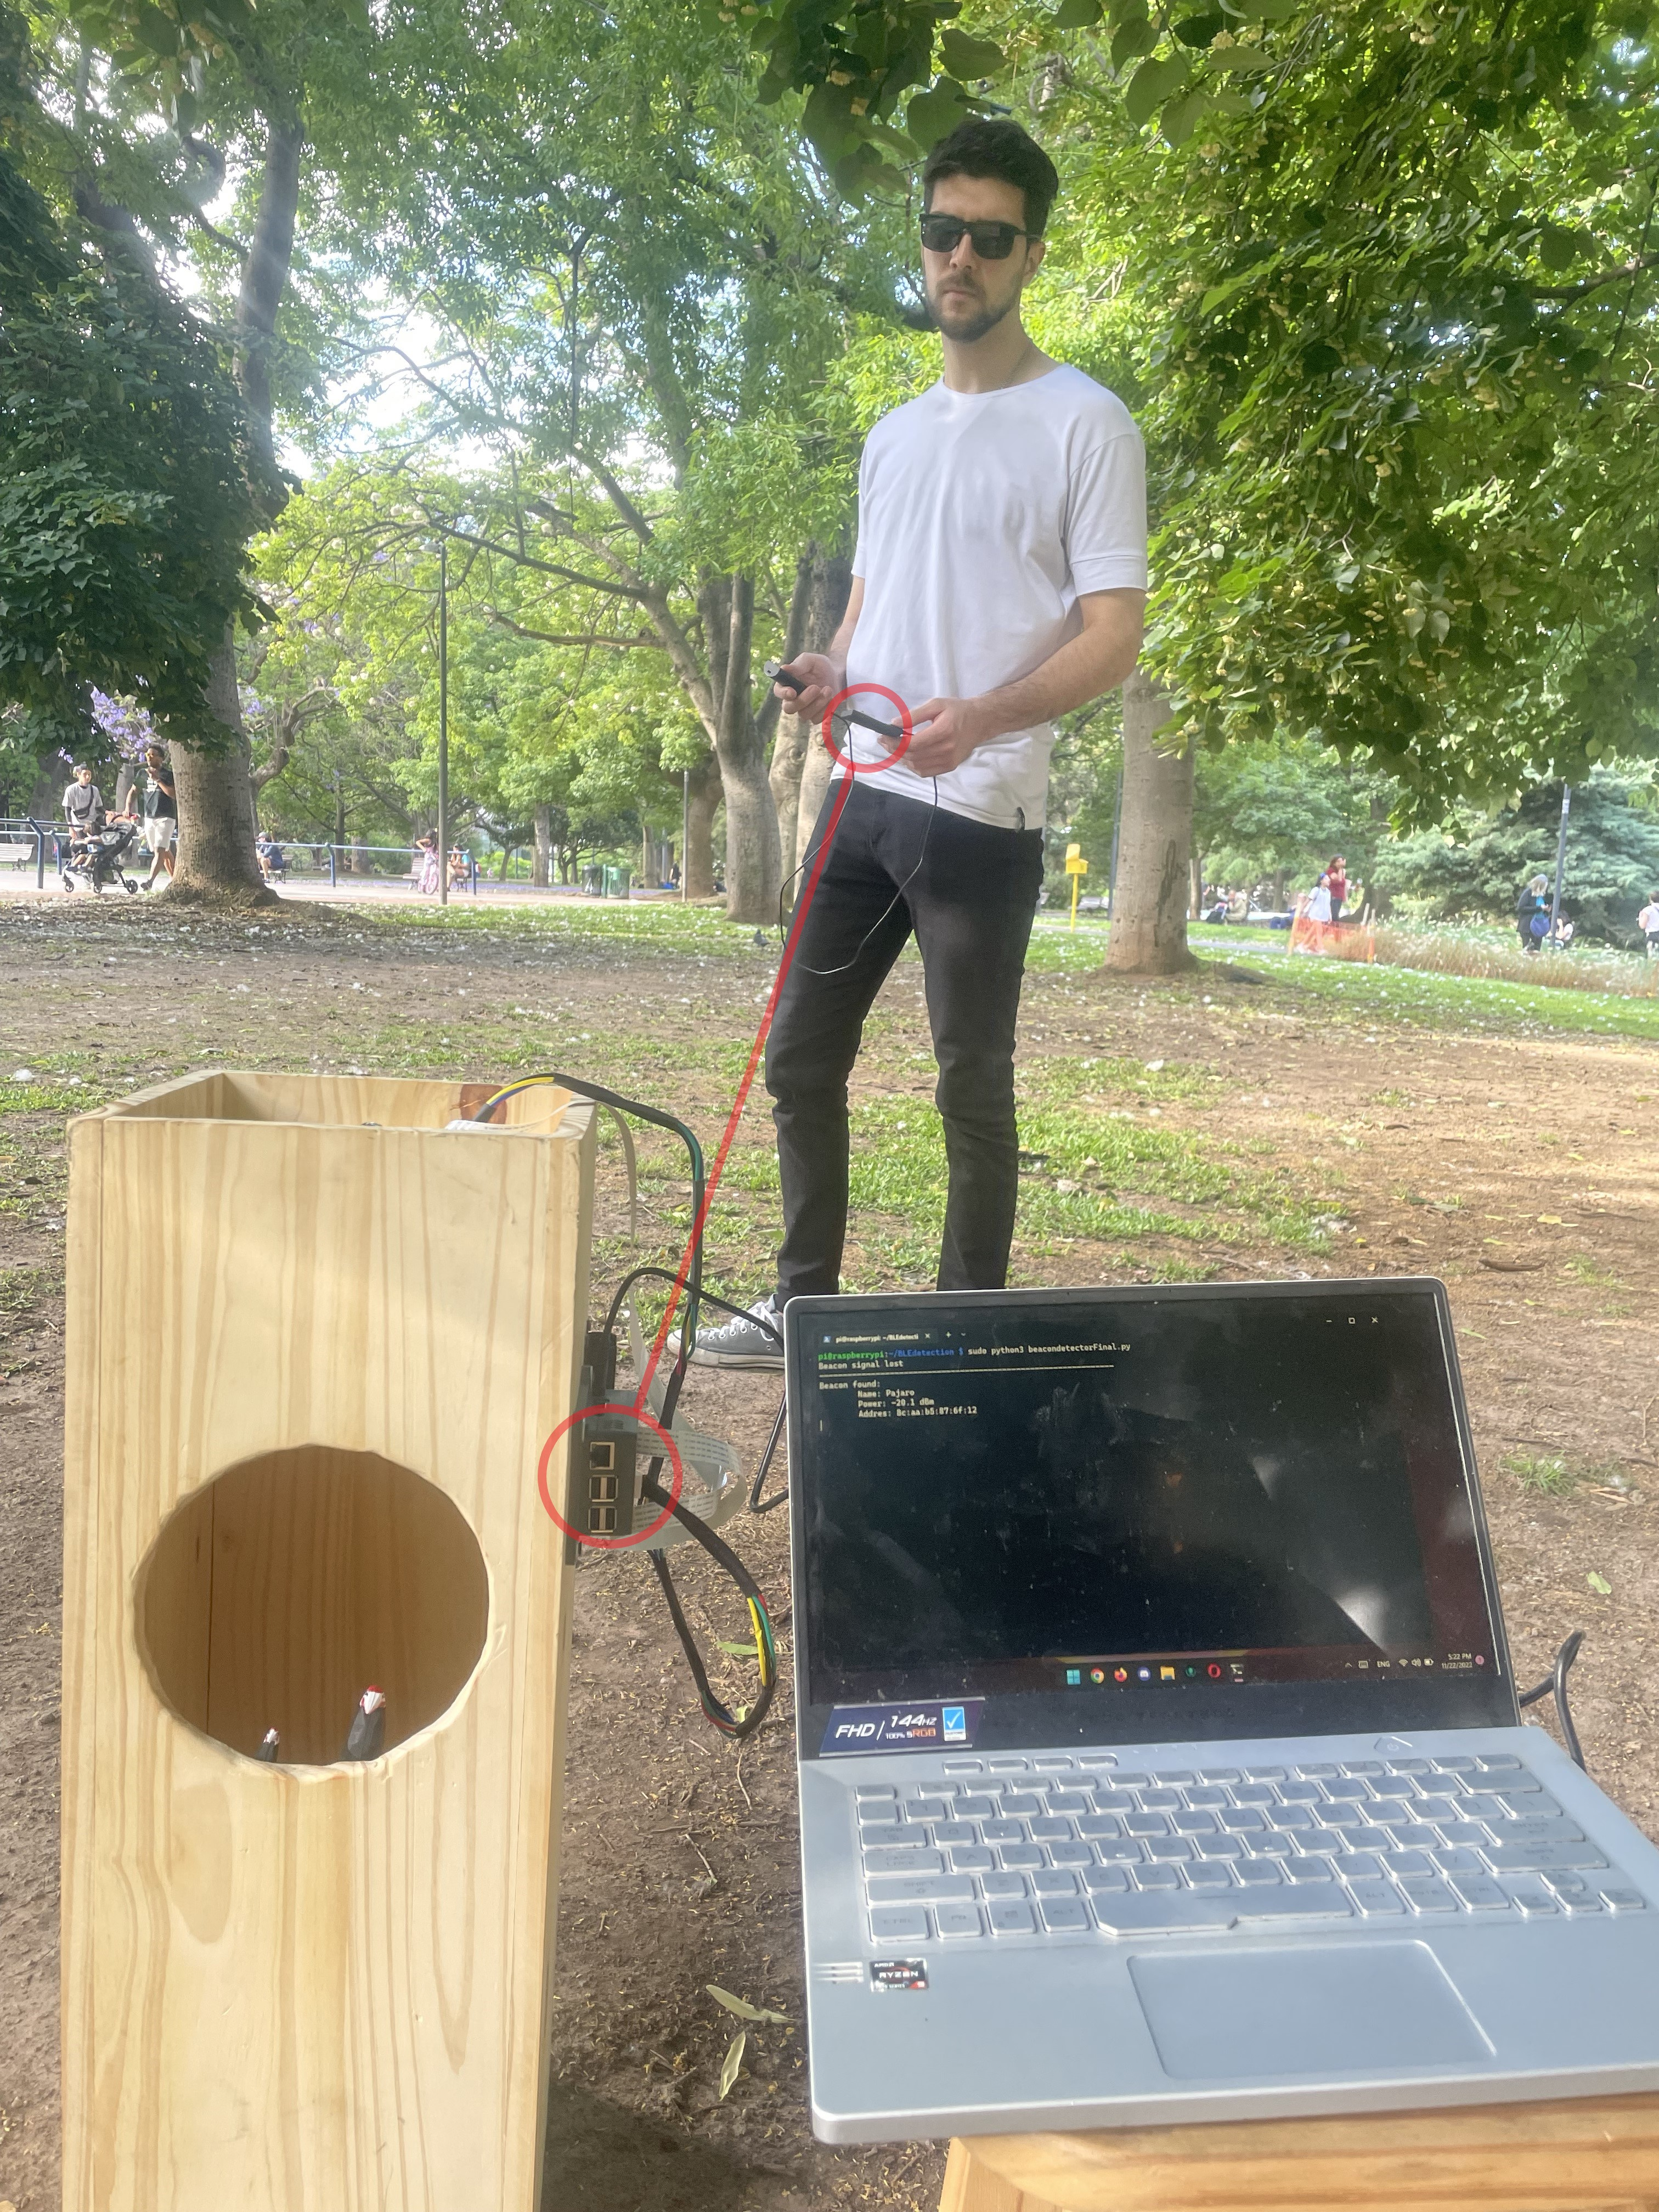
\includegraphics[width=\linewidth]{ImagenesValidacion del prototipo/TINTCOM12a}
		\caption{Distancia de 1 metro.}
	\end{subfigure}	
\end{figure}
\begin{figure}[H]
	\centering
	\ContinuedFloat
	\begin{subfigure}{0.3\textwidth}
		\centering
		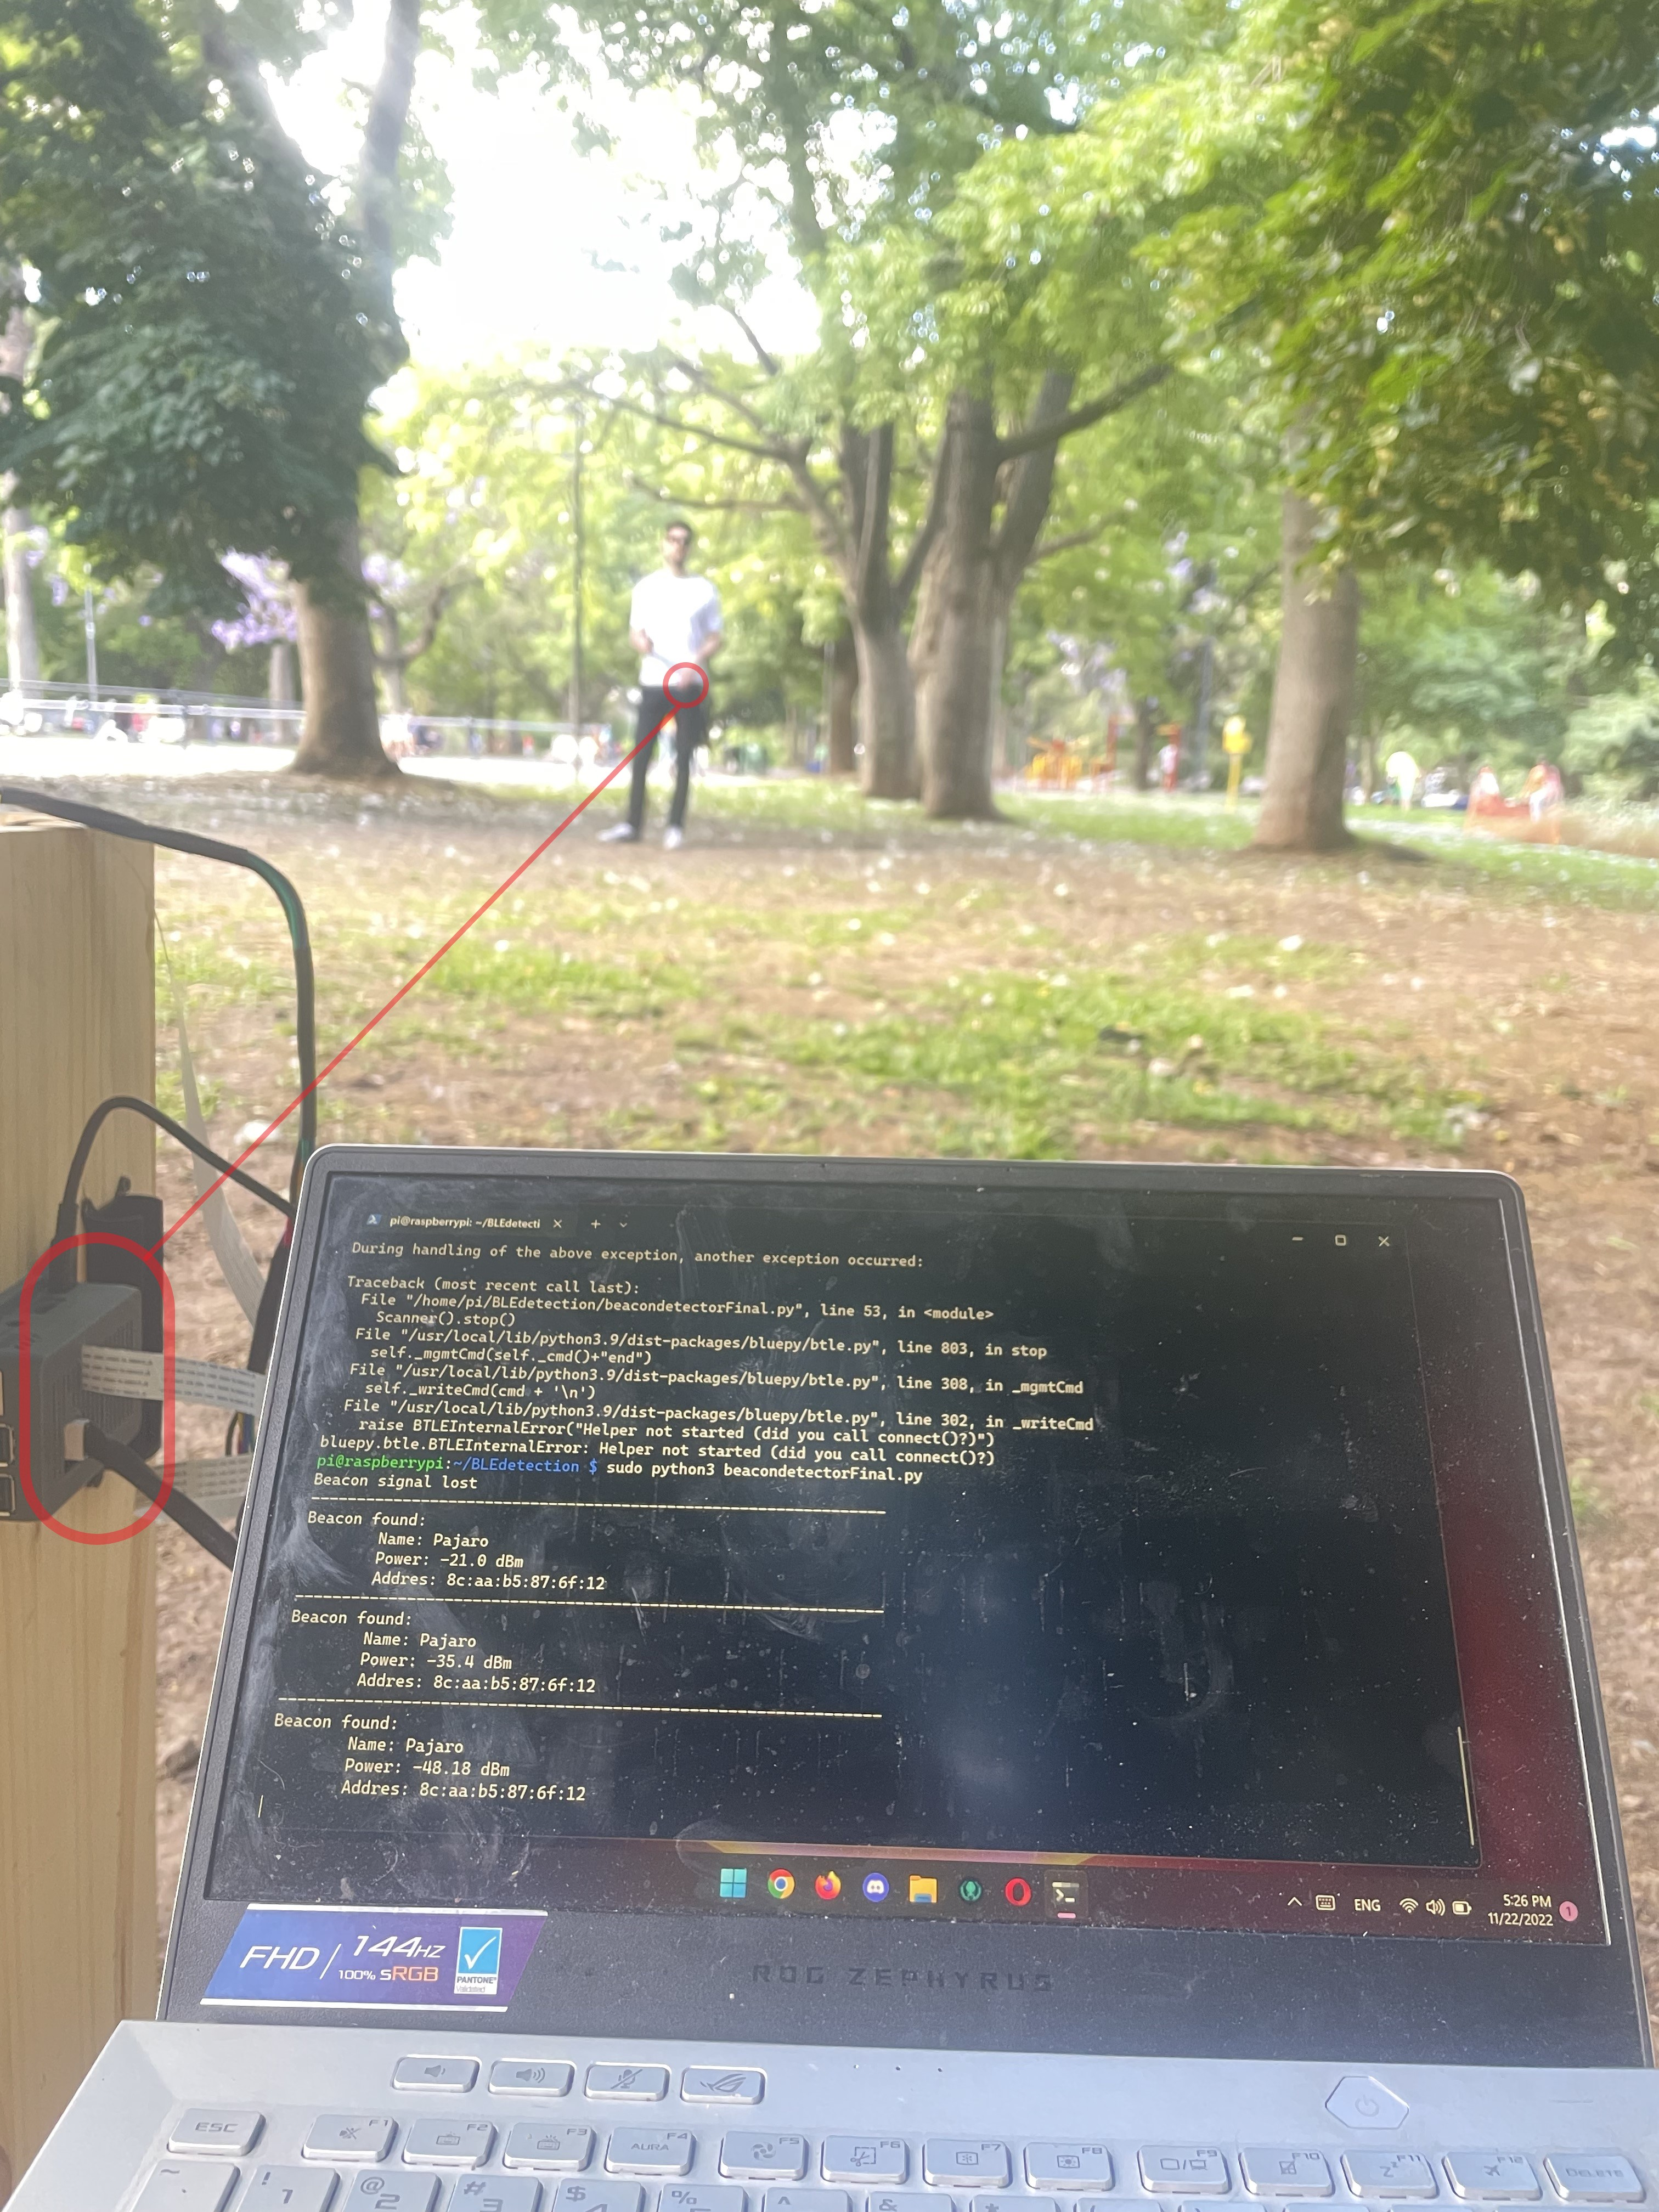
\includegraphics[width=\linewidth]{ImagenesValidacion del prototipo/TINTCOM12ba}		
		\caption{Distancia de 15 metros.}
	\end{subfigure}\hspace*{2.5cm}
	\begin{subfigure}{0.3\textwidth}
		\centering
		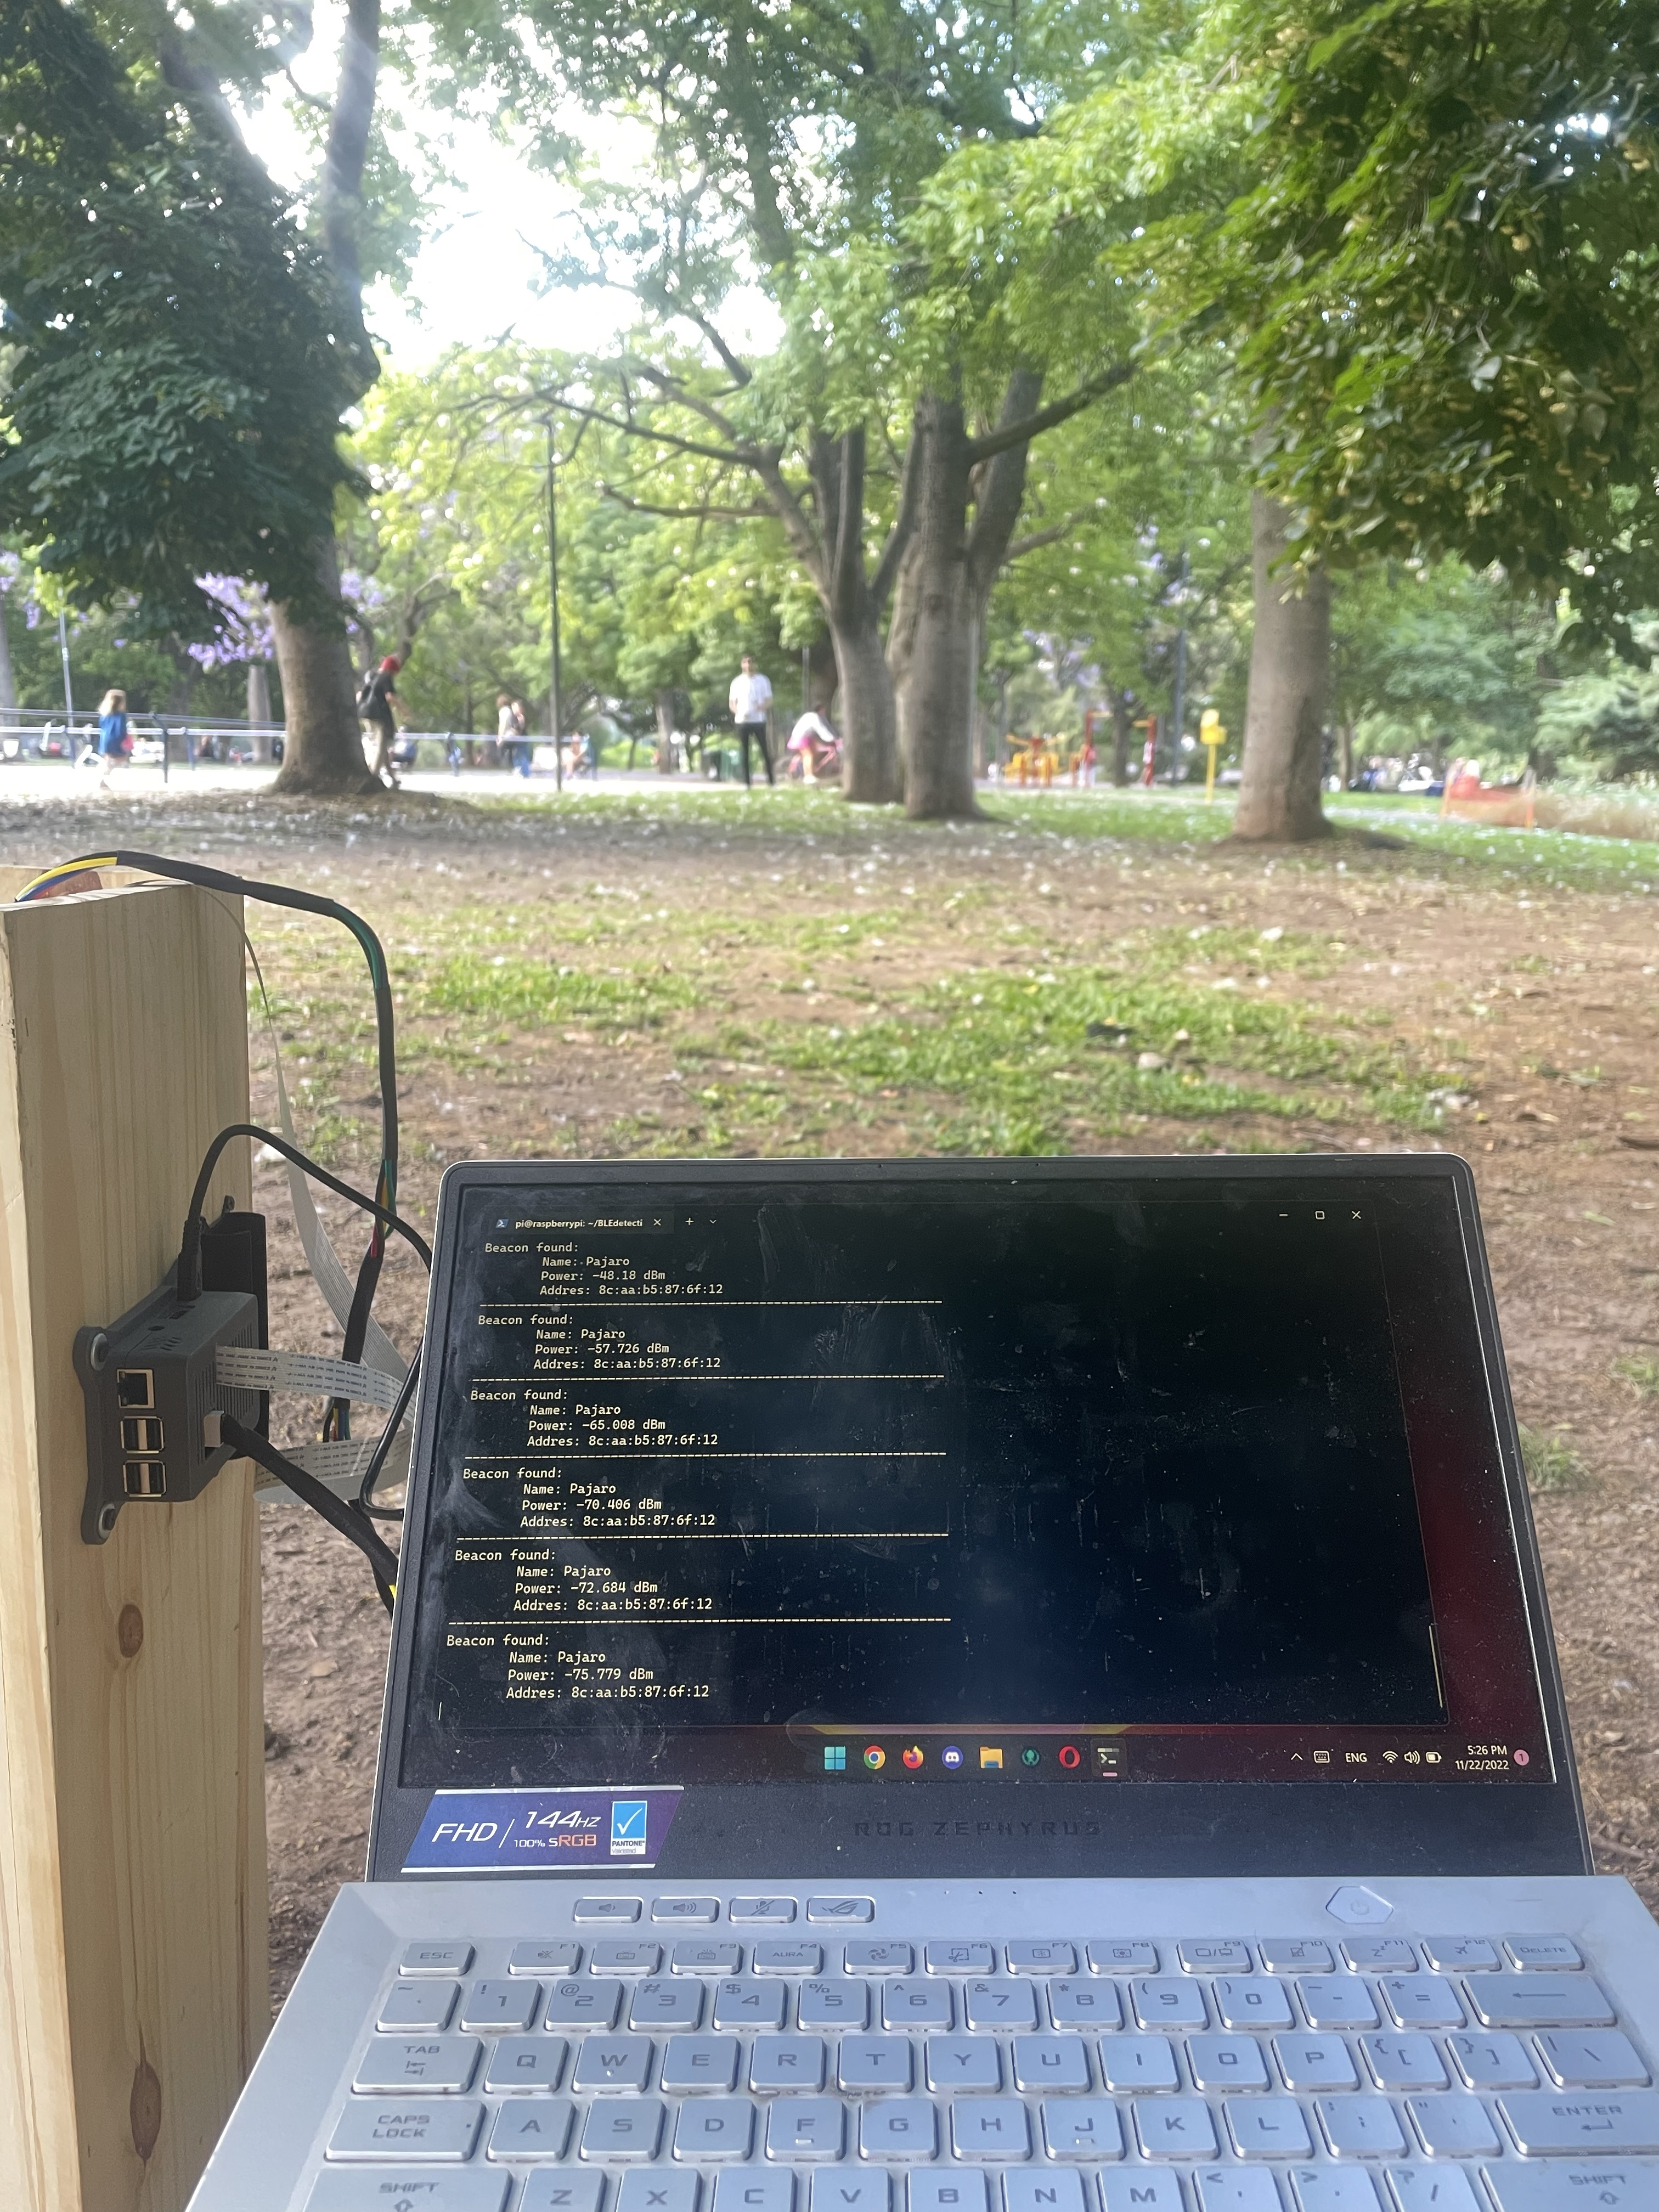
\includegraphics[width=\linewidth]{ImagenesValidacion del prototipo/TINTCOM12ca}
		\caption{Distancia de 30 metros.}
	\end{subfigure}
	\caption{Validación \textit{T-COM1-02}.}
\end{figure}

\Subsection{Validación Pruebas de Comunicación 2}
Para las pruebas de Comunicación 2 se requiere la computadora de un tercero (biólogo en campo). La primera prueba corresponde a \textit{T-INT-COM2-01} la cual consta en analizar a la capacidad de acceder a los datos del ave guardados en el nido.
\begin{figure}[H]
	\centering
	\begin{subfigure}{0.49\textwidth}
		\centering
		\includegraphics[width=\linewidth]{ImagenesValidacion del prototipo/TINTCOM21a}		
		\caption{Pestaña de descargas.}
	\end{subfigure}\hfill
	\begin{subfigure}{0.49\textwidth}
		\centering
		\includegraphics[width=\linewidth]{ImagenesValidacion del prototipo/TINTCOM21b}
		\caption{Botón de descarga.}
	\end{subfigure}
	\caption*{}
\end{figure}
\begin{figure}[H]
	\ContinuedFloat
	\centering
	\begin{subfigure}{\textwidth}
		\centering
		\includegraphics[width=0.8\linewidth]{ImagenesValidacion del prototipo/TINTCOM21}
		\caption{Consola y csv descargado.}
	\end{subfigure}
	\caption{Validación de comunicación \textit{T-INT-COM2-01}.}
\end{figure}

Se observa que los datos descargados que se ven en la izquierda se corresponden con los datos que se encuentran en el nido como se ve a la derecha. Por lo que no hubo una pérdida de datos.
Adicionalmente se utilizó una función de \textit{hash} para comparar los contenidos de ambos archivos y fehacientemente comprobar que son el mismo archivo. 

Por su parte, el desarrollo de las pruebas de \textit{T-INT-COM2-02} se efectuó sin mayores inconvenientes, logrando la conexión continua variando la distancia en rango de 4 a 14 metros.
\begin{figure}[H]
\centering	\includegraphics[width=0.6\linewidth]{ImagenesValidacion del prototipo/TINTCOM22}
	\caption{Validación de funcionalidad \textit{T-INT-COM2-02}.}
\end{figure}

Finalmente con lo que respecta a los bancos de prueba de comunicación, se procede a realizar la validación correspondiente a \textit{T-INT-COM2-03}. En esta prueba se de verificar la existencia del archivo \textit{BirdData} luego descargarlo y al acceder nuevamente a la \rspi comprobar que este fue borrado exitosamente.
\begin{figure}[H]
\centering
	\includegraphics[width=1\linewidth]{ImagenesValidacion del prototipo/TINTCOM23}
	\caption{Validación de comunicación \textit{T-INT-COM2-3}.}
\end{figure}

\Subsection{Validación pruebas de seguridad}
Se dispuso del banco de pruebas \#1 para analizar la aplicabilidad de \textit{T-RAM-SEG-01}. El acceso tanto a la interfaz gráfica del usuario como la del administrador se encuentran restringidas para cualquiera que no posea las credenciales adecuadas.
\begin{figure}[H]
\centering
    	\begin{subfigure}{0.49\textwidth}
        	\centering
        	\includegraphics[width=\linewidth]{ImagenesValidacion del prototipo/t-ram-seg-01-1}		
			\caption{Autenticación de usuario para la interfaz gráfica.}
        \end{subfigure}\hfill
        \begin{subfigure}{0.49\textwidth}
        	\centering
        	\includegraphics[width=\linewidth]{ImagenesValidacion del prototipo/t-ram-seg-01-2}
        	\caption{Autenticación de administrador para la interfaz gráfica.}
        \end{subfigure}
	\caption{Validación de seguridad \textit{T-RAM-SEG-01}.}
\end{figure}

Se obtuvo un resultado mejor del esperado ya que el hecho de emplear una red WiFi para conectar la unidad del nido con el usuario también requiere del uso de una contraseña. Esto agrega una capa de seguridad extra al sistema.


\Section{Estudios de Confiabilidad de Hardware y de Software}
%\documentclass[a4paper]{article}
%\usepackage[utf8]{inputenc}
\usepackage[spanish, es-tabla, es-noshorthands]{babel}
\usepackage[table,xcdraw,dvipsnames]{xcolor}
\usepackage[a4paper, footnotesep=1.25cm, headheight=1.25cm, top=2.54cm, left=2.54cm,
 bottom=2.54cm, right=2.54cm]{geometry}
%\geometry{showframe}
 \usepackage[normalem]{ulem}
 \useunder{\uline}{\ul}{}

%VERIFICAR EL HEAD Y EL FOOT EN
%https://ctan.dcc.uchile.cl/macros/latex/contrib/geometry/geometry.pdf

%Paquetes varios:
\usepackage{verbatimbox}

%\usepackage{wrapfig}			%Wrap figure in text
\usepackage[export]{adjustbox}	%Move images
\usepackage{changepage}			%Move tables
\usepackage{todonotes}

\usepackage{tikz}
\usepackage{amsmath}
\usepackage{amsfonts}
\usepackage{amssymb}
\usepackage{float}
\usepackage[graphicx]{realboxes}
\usepackage{caption}
\usepackage{subcaption}
\usepackage{multicol}
\usepackage{multirow}
\setlength{\doublerulesep}{\arrayrulewidth}
%\usepackage{booktabs}

\usepackage{array}
\newcolumntype{C}[1]{>{\centering\let\newline\\\arraybackslash\hspace{0pt}}m{#1}}
%\usepackage[american]{circuitikz}
\usetikzlibrary{calc}
\usepackage{fancyhdr}
\usepackage{units} 

\usepackage{colortbl}
%\usepackage{sectsty}
%\usepackage{unicode-math}

%FONTS (IMPORTANTE): Compilar en XeLaTex o LuaLaTeX
\usepackage{anyfontsize}	%Font size
\usepackage{fontspec}		%Font type
%Si sigue sin andar comentar \usepackage[utf8]{inputenc}
%https://ctan.dcc.uchile.cl/macros/unicodetex/latex/fontspec/fontspec.pdf
%https://www.overleaf.com/learn/latex/XeLaTeX

%Path para imagenes para trabajar en subarchivos
\graphicspath{{../Resumen/}{../Referencias/}{../Apendice/}{../Descripción de la Empresa/}{../Tareas del Alumno/}{../Conclusiones/}{../Herramientas Empleadas/}}

%Definiciones de nuevos comandos y colores
%COLORES:
\definecolor{AzulFoot}{rgb}{0.682,0.809,0.926}	%RGB	%{174,206,235}
\definecolor{AzulInfo}{rgb}{0.180,0.455,0.710}	%RGB	%{46,116,181}
\definecolor{AzulTable}{rgb}{0.302,0.507,0.871}	%RGB	%{68,114,196}
\definecolor{PName}{rgb}{0.353,0.353,0.353}		%RGB	%{90,90,90}
\definecolor{mygreen}{rgb}{28,172,0} % color values Red, Green, Blue
\definecolor{mylilas}{rgb}{170,55,241}

%Change Font Size

% #1 = size, #2 = text
\newcommand{\setparagraphsize}[2]{{\fontsize{#1}{6}\selectfont#2 \par}}		%Cambia el size de todo el parrafo
\newcommand{\setlinesize}[2]{{\fontsize{#1}{6}\selectfont#2}}				%Cambia el font de una oración

%IMAGE IN TABLE:			%Ejemplo: \includeintable{.3}{ImagenesFactibilidad/pend}
\renewcommand\fbox{\fcolorbox{white}{white}}
\setlength{\fboxrule}{0pt}	%padding thickness
\setlength{\fboxsep}{4pt}	%border thickness
\newcommand{\includeintable}[2]{	
	\fbox{
		\begin{minipage}{#1\textwidth}
        	\includegraphics[width=\linewidth]{#2}
    	\end{minipage}
	}
}

%LINK IN REF
\newcommand{\reflink}[1]{		%LINK
	\href{#1}{#1}
}

%NOTAS:
\newcommand{\note}[1]{		%RED BIG NOTE (TODO)
	\begin{center}
		\huge{ \textcolor{red}{#1} }
	\end{center}
}

\newcommand{\lnote}[1]{{\fontsize{14}{6}\selectfont\textcolor{green}{#1}}}	%Notas pequeñas

\newcommand{\observacion}[2]{  \ifnumequal{1}{#1}{ { \todo[inline,backgroundcolor=red!25,bordercolor=red!100]{\textbf{Observación: #2}} } }{  }  }

\newcommand{\red}[1]{\textcolor{red}{#1}}

\newcommand{\TBD}{\textcolor{red}{(TBD) }}
\newcommand{\tbd}{\textcolor{red}{(TBD) }}

\newcommand{\TBC}{\textcolor{red}{(TBC) }}
\newcommand{\tbc}{\textcolor{red}{(TBC) }}

\newcommand{\quotes}[1]{``#1''}
\newcommand{\q}[1]{``#1''}

\newcommand{\ip}{192.168.0.10:1880}
\newcommand{\ipadmin}{192.168.0.10:1880/admin}

% Comandos para agregar elementos en tablas de acronimos y definiciones
\newcommand{\addacronym}[2]{\textbf{#1} & \begin{tabular}[l]{@{}l@{}}#2\end{tabular} \\ \hline}

% tabItem
\newcommand{\tabitem}{~~\llap{\textbullet}~~}


\usepackage{hyperref}
\hypersetup{
    colorlinks=true,
    linkcolor=black,
    filecolor=magenta,      
    urlcolor=AzulInfo,
    citecolor=AzulInfo,    
}

%Configuración del header y del footer:
\usepackage{etoolbox}
\pagestyle{fancy}
\fancyhf{}
\rfoot{\thepage}
\renewcommand{\footrulewidth}{4pt}
\renewcommand{\headrulewidth}{0pt}
\patchcmd{\footrule}{\hrule}{\color{AzulFoot}\hrule}{}{}

%Código en el informe
%% IMPORTANTE:
% Verificar que esté \usepackage[dvipsnames]{xcolor}

%\usepackage{listingsutf8}
\usepackage{listings}

\renewcommand{\lstlistingname}{Código}

%LSTSET: Pone un recuadro y contador de linea en el codigo
\newcommand{\boxstyle}{
	\lstset{
		basicstyle=\sffamily\color{black},
		frame=single,
		numbers=left,
		numbersep=5pt,
		numberstyle=\color{gray},
		showspaces=false,
		showstringspaces=false
	}
}

\newcommand{\defaultstyle}{
	\lstset{
		basicstyle=\sffamily\color{white},
		frame=none,
		numbers=none,
		showspaces=true,
		showstringspaces=true
	}
}

\lstdefinelanguage{Kotlin}{
  captionpos=b,
  comment=[l]{//},
  commentstyle={\color{gray}\ttfamily},
  emph={filter, first, firstOrNull, forEach, lazy, map, mapNotNull, println},
  emphstyle={\color{OrangeRed}},
  identifierstyle=\color{black},
  keywords={!in, !is, abstract, actual, annotation, as, as?, break, by, catch, class, companion, const, constructor, continue, crossinline, data, delegate, do, dynamic, else, enum, expect, external, false, field, file, final, finally, for, fun, get, if, import, in, infix, init, inline, inner, interface, internal, is, lateinit, noinline, null, object, open, operator, out, override, package, param, private, property, protected, public, receiveris, reified, return, return@, sealed, set, setparam, super, suspend, tailrec, this, throw, true, try, typealias, typeof, val, var, vararg, when, where, while},
  keywordstyle={\color{NavyBlue}\bfseries},
  morecomment=[s]{/*}{*/},
  morestring=[b]",
  morestring=[s]{"""*}{*"""},
  ndkeywords={@Deprecated, @JvmField, @JvmName, @JvmOverloads, @JvmStatic, @JvmSynthetic, Array, Byte, Double, Float, Int, Integer, Iterable, Long, Runnable, Short, String, Any, Unit, Nothing},
  ndkeywordstyle={\color{BurntOrange}\bfseries},
  sensitive=true,
  stringstyle={\color{ForestGreen}\ttfamily},
}

\lstdefinelanguage{Swift}
{
  morekeywords={
    open,catch,@escaping,nil,throws,func,if,then,else,for,in,while,do,switch,case,default,where,break,continue,fallthrough,return,
    typealias,struct,class,enum,protocol,var,func,let,get,set,willSet,didSet,inout,init,deinit,extension,
    subscript,prefix,operator,infix,postfix,precedence,associativity,left,right,none,convenience,dynamic,
    final,lazy,mutating,nonmutating,optional,override,required,static,unowned,safe,weak,internal,
    private,public,is,as,self,unsafe,dynamicType,true,false,nil,Type,Protocol,
  },
  morecomment=[l]{//}, % l is for line comment
  morecomment=[s]{/*}{*/}, % s is for start and end delimiter
  morestring=[b]", % defines that strings are enclosed in double quotes
  breaklines=true,
  escapeinside={\%*}{*)},
  numbers=left,
  captionpos=b,
  breakatwhitespace=true,
  basicstyle=\linespread{1.0}\ttfamily, % https://tex.stackexchange.com/a/102728/129441
}

\definecolor{keyword}{HTML}{BA2CA3}
\definecolor{string}{HTML}{D12F1B}
\definecolor{comment}{HTML}{008400}

\newcommand{\swiftstyle}{
	\lstset{
  		language=Swift,
  		inputencoding=utf8x,
		extendedchars=\true,
	  	basicstyle=\ttfamily,
	  	showstringspaces=false, % lets spaces in strings appear as real spaces
  		columns=fixed,
  		keepspaces=true,
  		keywordstyle=\color{keyword},
  		stringstyle=\color{string},
  		commentstyle=\color{comment}
	}
}


%Como usarlo:

%\begin{lstlisting}[caption={Simple code listing.}, label={lst:example1}, language=Kotlin]
%// this is a simple code listing:
%println("hello kotlin from latex")
%\end{lstlisting}

%Si se corta en 2 páginas distintas:

%\vspace{1mm}
%\noindent{\begin{minipage}{\linewidth}
%\begin{lstlisting}[...]
%...
%\end{lstlisting}
%\end{minipage}}




\usepackage{titlesec}		%Para hacer las subsubsubsections

%Colores a los nombres de las secciones:
%\sectionfont{\color{AzulInfo}}  % sets color of sections
%\subsectionfont{\color{AzulInfo}}
%\subsubsectionfont{\color{AzulInfo}}

%PICTURES AND TABLE INDEX:
\newcommand{\Section}[1]{ \section{#1} 
	\phantomsection \setcounter{figure}{0} \setcounter{table}{0} \setcounter{lstlisting}{0}
		\renewcommand{\thetable}{\arabic{section}.\arabic{table}}
		\renewcommand{\thefigure}{\arabic{section}.\arabic{figure}}
		\renewcommand{\thelstlisting}{\arabic{section}.\arabic{lstlisting}}
}

\newcommand{\Subsection}[1]{ \subsection{#1}
	\phantomsection \setcounter{figure}{0} \setcounter{table}{0} \setcounter{lstlisting}{0}
		\renewcommand{\thetable}{\arabic{section}.\arabic{subsection}.\arabic{table}}
		\renewcommand{\thefigure}{\arabic{section}.\arabic{subsection}.\arabic{figure}}
		\renewcommand{\thelstlisting}{\arabic{section}.\arabic{subsection}.\arabic{lstlisting}}
}

\newcommand{\Subsubsection}[1]{ \subsubsection{#1} 
	\phantomsection \setcounter{figure}{0} \setcounter{table}{0}  \setcounter{lstlisting}{0}
		\renewcommand{\thetable}{\arabic{section}.\arabic{subsection}.\arabic{subsubsection}.\arabic{table}}
		\renewcommand{\thefigure}{\arabic{section}.\arabic{subsection}.\arabic{subsubsection}.\arabic{figure}}
		\renewcommand{\thelstlisting}{\arabic{section}.\arabic{subsection}.\arabic{subsubsection}.\arabic{lstlisting}}
}

%Definición de subsubsubsection:
\titleclass{\subsubsubsection}{straight}[\subsection]

\newcounter{subsubsubsection}[subsubsection]
\renewcommand\thesubsubsubsection{\thesubsubsection.\arabic{subsubsubsection}}

\titleformat{\subsubsubsection}
  {\normalfont\normalsize\bfseries\color{AzulInfo}}{\thesubsubsubsection}{1em}{}	%Color de subsubsubsection
\titlespacing*{\subsubsubsection}
{0pt}{3.25ex plus 1ex minus .2ex}{1.5ex plus .2ex}

\makeatletter
\renewcommand\paragraph{\@startsection{paragraph}{5}{\z@}%
  {3.25ex \@plus1ex \@minus.2ex}%
  {-1em}%
  {\normalfont\normalsize\bfseries}}
\renewcommand\subparagraph{\@startsection{subparagraph}{6}{\parindent}%
  {3.25ex \@plus1ex \@minus .2ex}%
  {-1em}%
  {\normalfont\normalsize\bfseries}}
\def\toclevel@subsubsubsection{4}
\def\toclevel@paragraph{5}
\def\toclevel@paragraph{6}
\def\l@subsubsubsection{\@dottedtocline{4}{7em}{4em}}
\def\l@paragraph{\@dottedtocline{5}{10em}{5em}}
\def\l@subparagraph{\@dottedtocline{6}{14em}{6em}}
\makeatother

\setcounter{secnumdepth}{4}
\setcounter{tocdepth}{4}

%Subsubsubsection:
\newcommand{\Subsubsubsection}[1]{ \subsubsubsection{#1} 
	\phantomsection \setcounter{figure}{0} \setcounter{table}{0} \renewcommand{\thetable}{\arabic{section}.\arabic{subsection}.\arabic{subsubsection}.\arabic{subsubsubsection}.\arabic{table}} \renewcommand{\thefigure}{\arabic{section}.\arabic{subsection}.\arabic{subsubsection}.\arabic{subsubsubsection}.\arabic{figure}}
}

%Tamaño, color e identación de sección, subsección, subsubsección y subsubsubsección:
%La identación de las subsecciones está tambien en Index-cfg.tex para el toc, lot y lot en el index
\titleformat{\section}[block]{\fontsize{16}{6}\selectfont\bfseries\color{AzulInfo}}{\thesection.}{1em}{} 
\titleformat{\subsection}[block]{\hspace{2.5em}\fontsize{13}{6}\selectfont\color{AzulInfo}}{\thesubsection}{1em}{}
\titleformat{\subsubsection}[block]{\hspace{3.5em}\fontsize{12}{6}\selectfont\color{AzulInfo}}{\thesubsubsection}{1em}{}
\titleformat{\subsubsubsection}[block]{\hspace{4em}\fontsize{11}{6}\selectfont\color{AzulInfo}}{\thesubsubsubsection}{1em}{}

%Pone las refrencias en el indice
\usepackage[numbib, nottoc, notlot, notlof]{tocbibind}

%Pone toc, lof y lot en colores y elijo el titulo de estos
\addto\captionsspanish{
	\renewcommand\contentsname{Contenidos}
	\renewcommand\listfigurename{Lista de Figuras}
	\renewcommand\listtablename{Lista de Tablas}
}

%Agrega TOC al indice
\renewcommand{\tableofcontents}{
	\stepcounter{section}
	\addcontentsline{toc}{section}{\protect\numberline{\thesection}\textbf{Contenidos}}
	\tableofcontents
}

%Agrega LOF al indice
\renewcommand{\listoffigures}{
	\stepcounter{section}
	\addcontentsline{toc}{section}{\protect\numberline{\thesection}\textbf{Lista de Figuras}}
	\listoffigures
}

%Agrega LOT al indice
\renewcommand{\listoftables}{
	\stepcounter{section}
	\addcontentsline{toc}{section}{\protect\numberline{\thesection}\textbf{Lista de Tablas}}
	\listoftables
}

%Indices: cambio la separación de los numeros para que entren tablas y fotos
\usepackage{tocloft}
\setlength{\cftfignumwidth}{1.35cm}  % change numwidth from figures in lof
\setlength{\cfttabnumwidth}{1.35cm}  % change numwidth from tables in lot
\renewcommand{\cfttoctitlefont}{\Large\bfseries\color{AzulInfo}}
\renewcommand{\cftloftitlefont}{\Large\bfseries\color{AzulInfo}}
\renewcommand{\cftlottitlefont}{\Large\bfseries\color{AzulInfo}}

%Coloca lineas punteadas a las seciones en el TOC
\renewcommand{\cftsecleader}{\cftdotfill{\cftdotsep}}

%Items con bullets y no cuadrados
\renewcommand{\labelitemi}{\textbullet }


%\begin{document}
En esta sección se analiza la confiabilidad de los elementos de \textit{hardware} y \textit{software}, exponiendo en cada caso los criterios utilizados. A su vez se separa la parte de \textit{hardware} observando cada parte de manera individual para luego obtener un resultado en conjunto.

\Subsection{Hardware}	
El estudio se lleva a cabo según la norma MIL-HDBK-217F, la cual estima la cantidad de fallas en unidad de tiempo para diferentes tipos de componentes electrónicos. Este estándar tiene en cuenta factores como las condiciones de uso, temperatura.

El primer paso consiste en realizar un gráfico de todos los módulos considerados críticos que garantizan las funcionalidades fundamentales del producto. Esto se presenta en la Figura (\ref{fig:criticos}).
\begin{figure}[H]
	\centering
	\includegraphics[width=0.9\linewidth,page=1]{ImagenesEstudios/ModulosCriticos}		
	\caption{Módulos críticos de funcionamiento.}
	\label{fig:criticos}
\end{figure}
Se calcula una estimación de la confiabilidad de cada módulo utilizando una estrategia \quotes{Top-Down}. Se encuentra la tasa de falla de cada submódulo mediante un proceso multiplicativo a la tasa de fallos base provista por las distintas cargas a las que son sometidos los componentes.
No se cuenta con redundancias, por lo que el valor de confiabilidad del módulo estará dado por la confiabilidad en serie de cada uno de sus componentes.Para todos los cálculos se considera una temperatura de 16$^{\circ}$C, la cual es la temperatura media de la zona d estudio en el periodo del mismo.
\begin{table}[H]
\centering
\begin{tabular}{|c|c|}
\hline
\textbf{Tipo de componente}   & \textbf{Cálculo de tasa de fallos $\left[\frac{\text{failures}}{10^6 \cdot \text{hour}}\right]$}                                                                               \\ \hline
\textbf{Resistencia}          & $\lambda_p \ = \ \lambda_b \ \cdot \  \pi_T \ \cdot \ \pi_P \ \cdot \ \pi_S \ \cdot \ \pi_Q \ \cdot \ \pi_E$                                                                   \\ \hline
\textbf{Capacitor}            & $\lambda_p \ = \ \lambda_b \ \cdot \  \pi_T \ \cdot \ \pi_C \ \cdot \ \pi_V \ \cdot \ \pi_{SR} \ \cdot \ \pi_Q \ \cdot \ \pi_E  $                                              \\ \hline
\textbf{IC DHT-22}            & $\lambda_p \ = \  (C_1 \ \cdot \ \pi_T \ + \ C_2 \ \cdot \ \pi_E ) \cdot \ \pi_Q \ \cdot \ \pi_L  $                                                                            \\ \hline
\textbf{IC BH1750}            & $\lambda_p \ = \lambda_{BD} \ \cdot \ \pi_{MFG} \ \cdot \ \pi_T \ \cdot \ \pi_{CD} \ + \ \lambda_{BP} \ \cdot \ \pi_E \ \cdot \ \pi_Q + \lambda_{EOS}$                         \\ \hline
\textbf{Shield}               & $\lambda_p \ = \ \lambda_b \ \cdot \  \pi_T \ \cdot \ \pi_K  \ \cdot \ \pi_Q \ \cdot \ \pi_E $                                                                                 \\ \hline
\textbf{Conexionado Sensores} & $\lambda_p \ = \ \lambda_b \ \cdot \  \pi_T \ \cdot \ \pi_K  \ \cdot \ \pi_Q \ \cdot \ \pi_E $                                                                                 \\ \hline
\textbf{IC DS1307}            & $\lambda_p \ = \lambda_{BD} \ \cdot \ \pi_{MFG} \ \cdot \ \pi_T \ \cdot \ \pi_{CD} \ + \ \lambda_{BP} \ \cdot \ \pi_E \ \cdot \ \pi_Q + \lambda_{EOS}$                         \\ \hline
\textbf{Diodo}                & $\lambda_p \ = \ \lambda_b \ \cdot \  \pi_T \ \cdot \ \pi_S  \ \cdot \ \pi_C \ \cdot \ \pi_Q \ \cdot \ \pi_E $                                                                 \\ \hline
\textbf{Regulador de Tensión} & $\lambda_p \ = \ \lambda_b \ \cdot \  \pi_T \ \cdot \ \pi_S  \ \cdot \ \pi_C \ \cdot \ \pi_Q \ \cdot \ \pi_E $                                                                 \\ \hline
\textbf{Transistor Mosfet}    & $\lambda_p \ = \ \lambda_b \ \cdot \  \pi_T \ \cdot \ \pi_A  \ \cdot \ \pi_R \ \cdot \ \pi_S \ \cdot \ \pi_Q \ \cdot \ \pi_E $                                                 \\ \hline
\textbf{VHSIC}                & \cellcolor[HTML]{FFFFFF}$\lambda_p \ = \lambda_{BD} \ \cdot \ \pi_{MFG} \ \cdot \ \pi_T \ \cdot \ \pi_{CD} \ + \ \lambda_{BP} \ \cdot \ \pi_E \ \cdot \ \pi_Q + \lambda_{EOS}$ \\ \hline
\textbf{Batería}              & \multicolumn{1}{c|}{Documentación}                                                                                                                                             \\ \hline
\textbf{Panel Solar}          & \multicolumn{1}{c|}{Documentación}                                                                                                                                             \\ \hline
\textbf{Cámara \rspi}          & \multicolumn{1}{c|}{Documentación}                                                                                                                                             \\ \hline
\textbf{Inductor}             & \multicolumn{1}{c|}{\cellcolor[HTML]{FFFFFF}$\lambda_p \ = \ \lambda_b \ \cdot \ \pi_T  \ \pi_Q \ \cdot \ \pi_E$}                                                              \\ \hline
\textbf{ESP8266}              & $\lambda_p \ = \  (C_1 \ \cdot \ \pi_T \ + \ C_2 \ \cdot \ \pi_E ) \cdot \ \pi_Q \ \cdot \ \pi_L  $                                                                            \\ \hline
\textbf{\rspi}                & \multicolumn{1}{c|}{Documentación}                                                                                                                                             \\ \hline
\end{tabular}
\caption{Ecuaciones para obtener la tasa de fallos de cada módulo acorde a MIL-HDBK-217F.}
\label{tasadefallos}
\end{table}

\Subsubsection{\rspi}
Para el módulo \rspi se utiliza la documentación de esta para obtener el valor de la tasa de fallos.
\begin{equation}
\lambda_p = 3 
\end{equation}
\Subsubsection{Regulador de Energía}
\begin{table}[H]
\centering
\begin{tabular}{|c|ccc|}
\hline
\textbf{Componente}          & \multicolumn{1}{c|}{\textbf{Cantidad}} & \multicolumn{1}{c|}{$\boldsymbol{\lambda_p}$}        & $\boldsymbol{\lambda_{Tot}}$ \\ \hline
\textbf{Capacitor}           & \multicolumn{1}{c|}{9}                 & \multicolumn{1}{c|}{\cellcolor[HTML]{FFFFFF}0.00356} & 0.03204                      \\ \hline
\textbf{Resistor}            & \multicolumn{1}{c|}{36}                & \multicolumn{1}{c|}{\cellcolor[HTML]{FFFFFF}0.00267} & 0.09612                      \\ \hline
\textbf{Diodo}               & \multicolumn{1}{c|}{7}                 & \multicolumn{1}{c|}{\cellcolor[HTML]{FFFFFF}0.0007}  & 0.0049                       \\ \hline
\textbf{Inductor}            & \multicolumn{1}{c|}{2}                 & \multicolumn{1}{c|}{0.06138}                         & 0.12276                      \\ \hline
\textbf{Transistores MOSFET} & \multicolumn{1}{c|}{13}                & \multicolumn{1}{c|}{0.1776}                          & 2.3088                       \\ \hline
\textbf{IC Step-Down}        & \multicolumn{1}{c|}{1}                 & \multicolumn{1}{c|}{1.106}                           & 1.106                        \\ \hline
\textbf{IC MPPT}             & \multicolumn{1}{c|}{1}                 & \multicolumn{1}{c|}{1.017}                           & 1.017                        \\ \hline
\textbf{IC Protocolo USB}    & \multicolumn{1}{c|}{1}                 & \multicolumn{1}{c|}{1.004}                           & 1.004                        \\ \hline
\textbf{Total}               & \multicolumn{1}{l}{}                   & \multicolumn{1}{l}{}                                 & \multicolumn{1}{r|}{5.69162} \\ \hline
\end{tabular}
\caption{Confiabilidad regulador de energía.}
\label{confReg}
\end{table}

\Subsubsection{Paneles Solares}
Para determinar a tasa de fallas de los paneles solares se utiliza la documentación de estos.
\begin{equation}
\lambda_p = 0.057 
\end{equation}

\Subsubsection{Baterías}
Para determinar a tasa de fallas de las baterías se utiliza la documentación.
\begin{equation}
\lambda_p = 0.005 
\end{equation}
\Subsubsection{Conector Shield}
\begin{table}[H]
\centering
\begin{tabular}{|c|ccc|}
\hline
\textbf{Componente}     & \multicolumn{1}{c|}{\textbf{Cantidad}} & \multicolumn{1}{c|}{$\boldsymbol{\lambda_p}$}        & $\boldsymbol{\lambda_{Tot}}$ \\ \hline
\textbf{Conectores PCB} & \multicolumn{1}{c|}{1}                 & \multicolumn{1}{c|}{\cellcolor[HTML]{FFFFFF}0.00182} & 0.00182                      \\ \hline
\textbf{Conector Molex} & \multicolumn{1}{c|}{1}                 & \multicolumn{1}{c|}{\cellcolor[HTML]{FFFFFF}0.00182} & 0.00182                      \\ \hline
\textbf{Total}          & \multicolumn{1}{l}{}                   & \multicolumn{1}{l}{\cellcolor[HTML]{FFFFFF}}         & \multicolumn{1}{r|}{0.00364} \\ \hline
\end{tabular}
\caption{Confiabilidad de la placa \textit{shield}.}
\label{confshield}
\end{table}

\Subsubsection{RTC}
% Please add the following required packages to your document preamble:
% \usepackage[table,xcdraw]{xcolor}
% If you use beamer only pass "xcolor=table" option, i.e. \documentclass[xcolor=table]{beamer}
\begin{table}[H]
\centering
\begin{tabular}{|c|ccc|}
\hline
\textbf{Componente} & \multicolumn{1}{c|}{\textbf{Cantidad}} & \multicolumn{1}{c|}{$\boldsymbol{\lambda_p}$}        & $\boldsymbol{\lambda_{Tot}}$ \\ \hline
\textbf{Capacitor}  & \multicolumn{1}{c|}{3}                 & \multicolumn{1}{c|}{\cellcolor[HTML]{FFFFFF}0.00356} & 0.01068                      \\ \hline
\textbf{Resistor}   & \multicolumn{1}{c|}{5}                 & \multicolumn{1}{c|}{\cellcolor[HTML]{FFFFFF}0.00267} & 0.01335                      \\ \hline
\textbf{Diodo}      & \multicolumn{1}{c|}{1}                 & \multicolumn{1}{c|}{\cellcolor[HTML]{FFFFFF}0.0007}  & 0.0007                       \\ \hline
\textbf{DS1307}     & \multicolumn{1}{c|}{1}                 & \multicolumn{1}{c|}{1.106}                           & 1.106                        \\ \hline
\textbf{Total}      & \multicolumn{1}{l}{}                   & \multicolumn{1}{l}{}                                 & \multicolumn{1}{r|}{1.13073} \\ \hline
\end{tabular}
\caption{Confiabilidad RTC.}
\label{confRTC}
\end{table}
\Subsubsection{Sensor de Presencia}
% Please add the following required packages to your document preamble:
% \usepackage[table,xcdraw]{xcolor}
% If you use beamer only pass "xcolor=table" option, i.e. \documentclass[xcolor=table]{beamer}
\begin{table}[H]
\centering
\begin{tabular}{|c|ccc|}
\hline
\textbf{Componente}     & \multicolumn{1}{c|}{\textbf{Cantidad}} & \multicolumn{1}{c|}{$\boldsymbol{\lambda_p}$}     & $\boldsymbol{\lambda_{Tot}}$ \\ \hline
\textbf{ESP32 WROOM S3} & \multicolumn{1}{c|}{1}                 & \multicolumn{1}{c|}{\cellcolor[HTML]{FFFFFF}1.08} & 1.08                         \\ \hline
\textbf{Total}          & \multicolumn{1}{l}{}                   & \multicolumn{1}{l}{\cellcolor[HTML]{FFFFFF}}      & \multicolumn{1}{r|}{1.08}    \\ \hline
\end{tabular}
\caption{Confiabilidad sensor de presencia.}
\label{tab:confpres}
\end{table}
\Subsubsection{Cámara \rspi}
Para determinar la tasa de fallas del módulo de cámara se recurre a la hoja de datos.
\begin{equation}
\lambda_p = 3.16
\end{equation}
\Subsubsection{Conector Sensores}
\begin{table}[H]
\centering
\begin{tabular}{|c|clc|}
\hline
\textbf{Componente}     & \multicolumn{1}{c|}{\textbf{Cantidad}} & \multicolumn{1}{c|}{$\boldsymbol{\lambda_p}$} & $\boldsymbol{\lambda_{Tot}}$  \\ \hline
\textbf{Conector Molex} & \multicolumn{1}{c|}{1}                 & \multicolumn{1}{r|}{0.00182}              & 0.00182                      \\ \hline
\textbf{Total}          & \multicolumn{1}{l}{}                   &                                           & \multicolumn{1}{r|}{0.00182} \\ \hline
\end{tabular}
\caption{Confiabilidad Conector Placa de Sensores}
\label{confsensores}
\end{table}
\Subsubsection{Sensor Humedad y Temperatura}
% Please add the following required packages to your document preamble:
% \usepackage[table,xcdraw]{xcolor}
% If you use beamer only pass "xcolor=table" option, i.e. \documentclass[xcolor=table]{beamer}
\begin{table}[H]
\centering
\begin{tabular}{|c|crc|}
\hline
\textbf{Componente}         & \multicolumn{1}{c|}{\textbf{Cantidad}} & \multicolumn{1}{c|}{$\boldsymbol{\lambda_p}$}        & $\boldsymbol{\lambda_{Tot}}$ \\ \hline
\textbf{Capacitor} & \multicolumn{1}{c|}{2}                 & \multicolumn{1}{r|}{0.00356}                         & 0.00712                      \\ \hline
\textbf{Resistor}  & \multicolumn{1}{c|}{1}                 & \multicolumn{1}{r|}{\cellcolor[HTML]{FFFFFF}0.00267} & 0.00267                      \\ \hline
\textbf{IC-DHT22}  & \multicolumn{1}{c|}{1}                 & \multicolumn{1}{r|}{3.036}                           & 3.036                        \\ \hline
\textbf{Total}     & \multicolumn{1}{l}{}                   & \multicolumn{1}{l}{}                                 & \multicolumn{1}{r|}{3.04579} \\ \hline
\end{tabular}
\caption{Confiabilidad Sensor de Temperatura y Humedad.}
\label{tab:conftemphum}
\end{table}
\Subsubsection{Sensor Luminosidad}

\begin{table}[H]
\centering
\begin{tabular}{|c|crc|}
\hline
\textbf{Componente}           & \multicolumn{1}{c|}{\textbf{Cantidad}} & \multicolumn{1}{c|}{$\boldsymbol{\lambda_p}$}        & $\boldsymbol{\lambda_{Tot}}$ \\ \hline
\textbf{Capacitor}            & \multicolumn{1}{c|}{4}                 & \multicolumn{1}{r|}{0.00356}                         & 0.01424                      \\ \hline
\textbf{Resistor}             & \multicolumn{1}{c|}{3}                 & \multicolumn{1}{r|}{\cellcolor[HTML]{FFFFFF}0.00267} & 0.00801                      \\ \hline
\textbf{Regulador de tensión} & \multicolumn{1}{c|}{1}                 & \multicolumn{1}{r|}{\cellcolor[HTML]{FFFFFF}0.00059} & 0.00059                      \\ \hline
\textbf{IC-BH1750}            & \multicolumn{1}{c|}{1}                 & \multicolumn{1}{r|}{1.106}                           & 1.106                        \\ \hline
\textbf{Total}                & \multicolumn{1}{l}{}                   & \multicolumn{1}{l}{}                                 & \multicolumn{1}{r|}{1.12884} \\ \hline
\end{tabular}
\caption{Confiabilidad Sensor de Luminosidad}
\label{tab:conflum}
\end{table}

\Subsubsection{Tasa de fallas total}
Utilizando los valores finales obtenidos en las anteriores tablas se calcula el $\lambda_{Total}$ de la siguiente manera:
\begin{equation}
\lambda_{Total} \ = \  \sum_{Modulos} \  \lambda_{Totn}  \  =  \ 18.8174 \  \frac{\text{fallas}}{10^6 \ \text{horas}}
\end{equation}
Luego asumiendo que $\lambda$ es constante y la función de confiabilidad definida como:
\begin{equation}
R(t) \ = \ e^{-\frac{\lambda_{Total}}{10^6}\ \cdot t}
\end{equation}
Con esto definido se obtiene el tiempo medio a la falla para todo el sistema:
\begin{equation}
MTTF \ = \ \int_0^\infty \ R(t)\ dt \ \approx \ 53142.19 \ \text{horas} \ \approx \ 6.066 \ \text{años}
\end{equation}
Ademas, se calcula valores para R(T) con un paso de 3 meses (Duración base del proyecto) hasta 3 años.
\begin{table}[H]
\centering
\begin{tabular}{|c|c|c|c|c|c|c|}
\hline
\textbf{Tiempo} & \textbf{3 Meses}                                                    & \textbf{6 Meses} & \textbf{9 Meses}                                                    & \textbf{1 Año}                                                      & \textbf{\begin{tabular}[c]{@{}c@{}}1 Año y\\ 3 Meses\end{tabular}}   & \textbf{\begin{tabular}[c]{@{}c@{}}1 Año y\\ 6 Meses\end{tabular}} \\ \hline
\textbf{$R(t)$} & 0.96                                                                & 0.922            & 0.885                                                               & 0.850                                                               & 0.816                                                                & 0.786                                                              \\ \hline
\textbf{Tiempo} & \textbf{\begin{tabular}[c]{@{}c@{}}1 Año y \\ 9 Meses\end{tabular}} & \textbf{2 Años}  & \textbf{\begin{tabular}[c]{@{}c@{}}2 Años y\\ 3 Meses\end{tabular}} & \textbf{\begin{tabular}[c]{@{}c@{}}2 Años y\\ 6 Meses\end{tabular}} & \textbf{\begin{tabular}[c]{@{}c@{}}2 Años y \\ 9 Meses\end{tabular}} & \textbf{3 Años}                                                    \\ \hline
\textbf{$R(t)$} & 0.752                                                               & 0.722            & 0.70 & 0.677                                                               & 0.647                                                                & 0.622                                                            \\ \hline
\end{tabular}
\caption{Probabilidad de confiabilidad cada períodos de 3 meses.}
\label{probConf}
\end{table}

Teniendo en cuenta que el tiempo de vida del producto está estimado en 3 años y que la duración del estudio es de 3 meses. Que el tiempo medio a la falla sea de 6 años, resulta satisfactorio.
Finalmente cabe mencionar que luego de cada uso se recomienda una revisión técnica para asegurar un correcto funcionamiento de todos los módulos así aumentando la confiabilidad del sistema.
\Subsection{Software}
Para el estudio de confiabilidad de software se utilizó un modelo de estimación de tipo exponencial. Este modelo asume que todas las fallas que se presentan son independientes entre sí. Más específicamente se utilizará el modelo de Shooman, el cual normaliza las fallas por la cantidad de líneas de código $I_T$ sigue:
\begin{equation}
	R(t) = e^{-\lambda t}
\end{equation}
donde se toma
\begin{equation}
	\lambda = -k \left[ \epsilon_T - \epsilon(\zeta) \right]t
\end{equation}

Además, se define $\epsilon_T$ como la tasa de errores totales, $\epsilon(\zeta)$ la tasa de errores corregidos hasta un tiempo de corrección $\zeta$ y $k$ una constante del modelo de estimación.
\begin{table}[H]
\centering
\begin{tabular}{|c|c|c|c|c|c|c|c|c|}
\hline
\textbf{Semanas} & \boldmathcol{E_t}  		  & \boldmathcol{E_c}  			  & \boldmathcol{E_r}  			  & \textbf{H [hrs]} & \boldmathcol{\lambda_i}  & \boldmathcol{\frac{\lambda_i}{\lambda_{i-1}}}  & \boldmathcol{\hat{E}_{tot}}    & \boldmathcol{\hat{k}}    \\ \hline
1                & 20                         & 17                            & 3                             & 168              & 0.11905                  & -                                              & -                              & -                       \\ \hline
2                & 37                         & 33                            & 4                             & 336              & 0.05060                  & 0.42500                                        & 11.82609                       & 32.32474                \\ \hline
3                & 50                         & 43                            & 7                             & 504              & 0.02579                  & 0.50980                                        & 10.40000                       & 37.93184                \\ \hline
4                & 61                         & 52                            & 9                             & 672              & 0.01637                  & 0.63462                                        & 15.63158                       & 12.34174                \\ \hline
5                & 74                         & 65                            & 9                             & 840              & 0.01548                  & 0.94545                                        & 225.33333                      & 0.35769                 \\ \hline
6                & 89                         & 80                            & 9                             & 1008             & 0.01488                  & 0.96154                                        & 375.00000                      & 0.20329                 \\ \hline
7                & 105                        & 96                            & 9                             & 1176             & 0.01361                  & 0.91429                                        & 170.66667                      & 0.42079                 \\ \hline
8                & 115                        & 105                           & 10                            & 1344             & 0.00744                  & 0.54688                                        & 10.86207                       & 43.15476                \\ \hline
\end{tabular}
\caption{Fallas durante el periodo de \textit{testing} del \textit{software}.}
\label{tab:confsoft}
\end{table}

La Tabla (\ref{tab:confsoft}) presenta la cantidad acumulada de errores $E_t$, la cantidad acumulada de corregidos $E_c$, la cantidad acumulada resultante de los residuales $E_r$, las horas de \textit{testing} acumuladas \textbf{H [hrs]}, la tasa de fallos $\lambda$ y los parámetros invariables del modelo $\hat{E}_{tot}$ y $\hat{k}$ a lo largo del periodo de \textit{testing}. Estos son calculados mediante la formula:
\begin{equation}
	\hat{E}_{tot} = \frac{ \frac{\lambda_i}{\lambda_{i-1}} E_c(\tau_{i-1})-E_c(\tau_i)}{\frac{\lambda_i}{\lambda_{i-1}}-1}
\end{equation}
y
\begin{equation}
	\hat{k} = \lambda_i\frac{I_T}{\hat{E}_{tot}-E_c(\tau_i)}
\end{equation}

Finalmente, se adoptan los valores $\hat{E}_{tot} = 1$, $I_T = 5000$  y $\hat{k} = 43.15476$. Aproximando según
\begin{equation}
	\lambda = k\frac{E_r}{I_T}
\end{equation}
se obtiene $\lambda = 0.00863$ que, tomando el inverso de este valor se obtiene el $TMEF$, que resulta ser de $ 116 \ hs$.

%\end{document}


\Section{Conclusiones}
%\documentclass[a4paper]{article}
%\usepackage[utf8]{inputenc}
\usepackage[spanish, es-tabla, es-noshorthands]{babel}
\usepackage[table,xcdraw,dvipsnames]{xcolor}
\usepackage[a4paper, footnotesep=1.25cm, headheight=1.25cm, top=2.54cm, left=2.54cm,
 bottom=2.54cm, right=2.54cm]{geometry}
%\geometry{showframe}
 \usepackage[normalem]{ulem}
 \useunder{\uline}{\ul}{}

%VERIFICAR EL HEAD Y EL FOOT EN
%https://ctan.dcc.uchile.cl/macros/latex/contrib/geometry/geometry.pdf

%Paquetes varios:
\usepackage{verbatimbox}

%\usepackage{wrapfig}			%Wrap figure in text
\usepackage[export]{adjustbox}	%Move images
\usepackage{changepage}			%Move tables
\usepackage{todonotes}

\usepackage{tikz}
\usepackage{amsmath}
\usepackage{amsfonts}
\usepackage{amssymb}
\usepackage{float}
\usepackage[graphicx]{realboxes}
\usepackage{caption}
\usepackage{subcaption}
\usepackage{multicol}
\usepackage{multirow}
\setlength{\doublerulesep}{\arrayrulewidth}
%\usepackage{booktabs}

\usepackage{array}
\newcolumntype{C}[1]{>{\centering\let\newline\\\arraybackslash\hspace{0pt}}m{#1}}
%\usepackage[american]{circuitikz}
\usetikzlibrary{calc}
\usepackage{fancyhdr}
\usepackage{units} 

\usepackage{colortbl}
%\usepackage{sectsty}
%\usepackage{unicode-math}

%FONTS (IMPORTANTE): Compilar en XeLaTex o LuaLaTeX
\usepackage{anyfontsize}	%Font size
\usepackage{fontspec}		%Font type
%Si sigue sin andar comentar \usepackage[utf8]{inputenc}
%https://ctan.dcc.uchile.cl/macros/unicodetex/latex/fontspec/fontspec.pdf
%https://www.overleaf.com/learn/latex/XeLaTeX

%Path para imagenes para trabajar en subarchivos
\graphicspath{{../Resumen/}{../Referencias/}{../Apendice/}{../Descripción de la Empresa/}{../Tareas del Alumno/}{../Conclusiones/}{../Herramientas Empleadas/}}

%Definiciones de nuevos comandos y colores
%COLORES:
\definecolor{AzulFoot}{rgb}{0.682,0.809,0.926}	%RGB	%{174,206,235}
\definecolor{AzulInfo}{rgb}{0.180,0.455,0.710}	%RGB	%{46,116,181}
\definecolor{AzulTable}{rgb}{0.302,0.507,0.871}	%RGB	%{68,114,196}
\definecolor{PName}{rgb}{0.353,0.353,0.353}		%RGB	%{90,90,90}
\definecolor{mygreen}{rgb}{28,172,0} % color values Red, Green, Blue
\definecolor{mylilas}{rgb}{170,55,241}

%Change Font Size

% #1 = size, #2 = text
\newcommand{\setparagraphsize}[2]{{\fontsize{#1}{6}\selectfont#2 \par}}		%Cambia el size de todo el parrafo
\newcommand{\setlinesize}[2]{{\fontsize{#1}{6}\selectfont#2}}				%Cambia el font de una oración

%IMAGE IN TABLE:			%Ejemplo: \includeintable{.3}{ImagenesFactibilidad/pend}
\renewcommand\fbox{\fcolorbox{white}{white}}
\setlength{\fboxrule}{0pt}	%padding thickness
\setlength{\fboxsep}{4pt}	%border thickness
\newcommand{\includeintable}[2]{	
	\fbox{
		\begin{minipage}{#1\textwidth}
        	\includegraphics[width=\linewidth]{#2}
    	\end{minipage}
	}
}

%LINK IN REF
\newcommand{\reflink}[1]{		%LINK
	\href{#1}{#1}
}

%NOTAS:
\newcommand{\note}[1]{		%RED BIG NOTE (TODO)
	\begin{center}
		\huge{ \textcolor{red}{#1} }
	\end{center}
}

\newcommand{\lnote}[1]{{\fontsize{14}{6}\selectfont\textcolor{green}{#1}}}	%Notas pequeñas

\newcommand{\observacion}[2]{  \ifnumequal{1}{#1}{ { \todo[inline,backgroundcolor=red!25,bordercolor=red!100]{\textbf{Observación: #2}} } }{  }  }

\newcommand{\red}[1]{\textcolor{red}{#1}}

\newcommand{\TBD}{\textcolor{red}{(TBD) }}
\newcommand{\tbd}{\textcolor{red}{(TBD) }}

\newcommand{\TBC}{\textcolor{red}{(TBC) }}
\newcommand{\tbc}{\textcolor{red}{(TBC) }}

\newcommand{\quotes}[1]{``#1''}
\newcommand{\q}[1]{``#1''}

\newcommand{\ip}{192.168.0.10:1880}
\newcommand{\ipadmin}{192.168.0.10:1880/admin}

% Comandos para agregar elementos en tablas de acronimos y definiciones
\newcommand{\addacronym}[2]{\textbf{#1} & \begin{tabular}[l]{@{}l@{}}#2\end{tabular} \\ \hline}

% tabItem
\newcommand{\tabitem}{~~\llap{\textbullet}~~}


\usepackage{hyperref}
\hypersetup{
    colorlinks=true,
    linkcolor=black,
    filecolor=magenta,      
    urlcolor=AzulInfo,
    citecolor=AzulInfo,    
}

%Configuración del header y del footer:
\usepackage{etoolbox}
\pagestyle{fancy}
\fancyhf{}
\rfoot{\thepage}
\renewcommand{\footrulewidth}{4pt}
\renewcommand{\headrulewidth}{0pt}
\patchcmd{\footrule}{\hrule}{\color{AzulFoot}\hrule}{}{}

%Código en el informe
%% IMPORTANTE:
% Verificar que esté \usepackage[dvipsnames]{xcolor}

%\usepackage{listingsutf8}
\usepackage{listings}

\renewcommand{\lstlistingname}{Código}

%LSTSET: Pone un recuadro y contador de linea en el codigo
\newcommand{\boxstyle}{
	\lstset{
		basicstyle=\sffamily\color{black},
		frame=single,
		numbers=left,
		numbersep=5pt,
		numberstyle=\color{gray},
		showspaces=false,
		showstringspaces=false
	}
}

\newcommand{\defaultstyle}{
	\lstset{
		basicstyle=\sffamily\color{white},
		frame=none,
		numbers=none,
		showspaces=true,
		showstringspaces=true
	}
}

\lstdefinelanguage{Kotlin}{
  captionpos=b,
  comment=[l]{//},
  commentstyle={\color{gray}\ttfamily},
  emph={filter, first, firstOrNull, forEach, lazy, map, mapNotNull, println},
  emphstyle={\color{OrangeRed}},
  identifierstyle=\color{black},
  keywords={!in, !is, abstract, actual, annotation, as, as?, break, by, catch, class, companion, const, constructor, continue, crossinline, data, delegate, do, dynamic, else, enum, expect, external, false, field, file, final, finally, for, fun, get, if, import, in, infix, init, inline, inner, interface, internal, is, lateinit, noinline, null, object, open, operator, out, override, package, param, private, property, protected, public, receiveris, reified, return, return@, sealed, set, setparam, super, suspend, tailrec, this, throw, true, try, typealias, typeof, val, var, vararg, when, where, while},
  keywordstyle={\color{NavyBlue}\bfseries},
  morecomment=[s]{/*}{*/},
  morestring=[b]",
  morestring=[s]{"""*}{*"""},
  ndkeywords={@Deprecated, @JvmField, @JvmName, @JvmOverloads, @JvmStatic, @JvmSynthetic, Array, Byte, Double, Float, Int, Integer, Iterable, Long, Runnable, Short, String, Any, Unit, Nothing},
  ndkeywordstyle={\color{BurntOrange}\bfseries},
  sensitive=true,
  stringstyle={\color{ForestGreen}\ttfamily},
}

\lstdefinelanguage{Swift}
{
  morekeywords={
    open,catch,@escaping,nil,throws,func,if,then,else,for,in,while,do,switch,case,default,where,break,continue,fallthrough,return,
    typealias,struct,class,enum,protocol,var,func,let,get,set,willSet,didSet,inout,init,deinit,extension,
    subscript,prefix,operator,infix,postfix,precedence,associativity,left,right,none,convenience,dynamic,
    final,lazy,mutating,nonmutating,optional,override,required,static,unowned,safe,weak,internal,
    private,public,is,as,self,unsafe,dynamicType,true,false,nil,Type,Protocol,
  },
  morecomment=[l]{//}, % l is for line comment
  morecomment=[s]{/*}{*/}, % s is for start and end delimiter
  morestring=[b]", % defines that strings are enclosed in double quotes
  breaklines=true,
  escapeinside={\%*}{*)},
  numbers=left,
  captionpos=b,
  breakatwhitespace=true,
  basicstyle=\linespread{1.0}\ttfamily, % https://tex.stackexchange.com/a/102728/129441
}

\definecolor{keyword}{HTML}{BA2CA3}
\definecolor{string}{HTML}{D12F1B}
\definecolor{comment}{HTML}{008400}

\newcommand{\swiftstyle}{
	\lstset{
  		language=Swift,
  		inputencoding=utf8x,
		extendedchars=\true,
	  	basicstyle=\ttfamily,
	  	showstringspaces=false, % lets spaces in strings appear as real spaces
  		columns=fixed,
  		keepspaces=true,
  		keywordstyle=\color{keyword},
  		stringstyle=\color{string},
  		commentstyle=\color{comment}
	}
}


%Como usarlo:

%\begin{lstlisting}[caption={Simple code listing.}, label={lst:example1}, language=Kotlin]
%// this is a simple code listing:
%println("hello kotlin from latex")
%\end{lstlisting}

%Si se corta en 2 páginas distintas:

%\vspace{1mm}
%\noindent{\begin{minipage}{\linewidth}
%\begin{lstlisting}[...]
%...
%\end{lstlisting}
%\end{minipage}}




\usepackage{titlesec}		%Para hacer las subsubsubsections

%Colores a los nombres de las secciones:
%\sectionfont{\color{AzulInfo}}  % sets color of sections
%\subsectionfont{\color{AzulInfo}}
%\subsubsectionfont{\color{AzulInfo}}

%PICTURES AND TABLE INDEX:
\newcommand{\Section}[1]{ \section{#1} 
	\phantomsection \setcounter{figure}{0} \setcounter{table}{0} \setcounter{lstlisting}{0}
		\renewcommand{\thetable}{\arabic{section}.\arabic{table}}
		\renewcommand{\thefigure}{\arabic{section}.\arabic{figure}}
		\renewcommand{\thelstlisting}{\arabic{section}.\arabic{lstlisting}}
}

\newcommand{\Subsection}[1]{ \subsection{#1}
	\phantomsection \setcounter{figure}{0} \setcounter{table}{0} \setcounter{lstlisting}{0}
		\renewcommand{\thetable}{\arabic{section}.\arabic{subsection}.\arabic{table}}
		\renewcommand{\thefigure}{\arabic{section}.\arabic{subsection}.\arabic{figure}}
		\renewcommand{\thelstlisting}{\arabic{section}.\arabic{subsection}.\arabic{lstlisting}}
}

\newcommand{\Subsubsection}[1]{ \subsubsection{#1} 
	\phantomsection \setcounter{figure}{0} \setcounter{table}{0}  \setcounter{lstlisting}{0}
		\renewcommand{\thetable}{\arabic{section}.\arabic{subsection}.\arabic{subsubsection}.\arabic{table}}
		\renewcommand{\thefigure}{\arabic{section}.\arabic{subsection}.\arabic{subsubsection}.\arabic{figure}}
		\renewcommand{\thelstlisting}{\arabic{section}.\arabic{subsection}.\arabic{subsubsection}.\arabic{lstlisting}}
}

%Definición de subsubsubsection:
\titleclass{\subsubsubsection}{straight}[\subsection]

\newcounter{subsubsubsection}[subsubsection]
\renewcommand\thesubsubsubsection{\thesubsubsection.\arabic{subsubsubsection}}

\titleformat{\subsubsubsection}
  {\normalfont\normalsize\bfseries\color{AzulInfo}}{\thesubsubsubsection}{1em}{}	%Color de subsubsubsection
\titlespacing*{\subsubsubsection}
{0pt}{3.25ex plus 1ex minus .2ex}{1.5ex plus .2ex}

\makeatletter
\renewcommand\paragraph{\@startsection{paragraph}{5}{\z@}%
  {3.25ex \@plus1ex \@minus.2ex}%
  {-1em}%
  {\normalfont\normalsize\bfseries}}
\renewcommand\subparagraph{\@startsection{subparagraph}{6}{\parindent}%
  {3.25ex \@plus1ex \@minus .2ex}%
  {-1em}%
  {\normalfont\normalsize\bfseries}}
\def\toclevel@subsubsubsection{4}
\def\toclevel@paragraph{5}
\def\toclevel@paragraph{6}
\def\l@subsubsubsection{\@dottedtocline{4}{7em}{4em}}
\def\l@paragraph{\@dottedtocline{5}{10em}{5em}}
\def\l@subparagraph{\@dottedtocline{6}{14em}{6em}}
\makeatother

\setcounter{secnumdepth}{4}
\setcounter{tocdepth}{4}

%Subsubsubsection:
\newcommand{\Subsubsubsection}[1]{ \subsubsubsection{#1} 
	\phantomsection \setcounter{figure}{0} \setcounter{table}{0} \renewcommand{\thetable}{\arabic{section}.\arabic{subsection}.\arabic{subsubsection}.\arabic{subsubsubsection}.\arabic{table}} \renewcommand{\thefigure}{\arabic{section}.\arabic{subsection}.\arabic{subsubsection}.\arabic{subsubsubsection}.\arabic{figure}}
}

%Tamaño, color e identación de sección, subsección, subsubsección y subsubsubsección:
%La identación de las subsecciones está tambien en Index-cfg.tex para el toc, lot y lot en el index
\titleformat{\section}[block]{\fontsize{16}{6}\selectfont\bfseries\color{AzulInfo}}{\thesection.}{1em}{} 
\titleformat{\subsection}[block]{\hspace{2.5em}\fontsize{13}{6}\selectfont\color{AzulInfo}}{\thesubsection}{1em}{}
\titleformat{\subsubsection}[block]{\hspace{3.5em}\fontsize{12}{6}\selectfont\color{AzulInfo}}{\thesubsubsection}{1em}{}
\titleformat{\subsubsubsection}[block]{\hspace{4em}\fontsize{11}{6}\selectfont\color{AzulInfo}}{\thesubsubsubsection}{1em}{}

%Pone las refrencias en el indice
\usepackage[numbib, nottoc, notlot, notlof]{tocbibind}

%Pone toc, lof y lot en colores y elijo el titulo de estos
\addto\captionsspanish{
	\renewcommand\contentsname{Contenidos}
	\renewcommand\listfigurename{Lista de Figuras}
	\renewcommand\listtablename{Lista de Tablas}
}

%Agrega TOC al indice
\renewcommand{\tableofcontents}{
	\stepcounter{section}
	\addcontentsline{toc}{section}{\protect\numberline{\thesection}\textbf{Contenidos}}
	\tableofcontents
}

%Agrega LOF al indice
\renewcommand{\listoffigures}{
	\stepcounter{section}
	\addcontentsline{toc}{section}{\protect\numberline{\thesection}\textbf{Lista de Figuras}}
	\listoffigures
}

%Agrega LOT al indice
\renewcommand{\listoftables}{
	\stepcounter{section}
	\addcontentsline{toc}{section}{\protect\numberline{\thesection}\textbf{Lista de Tablas}}
	\listoftables
}

%Indices: cambio la separación de los numeros para que entren tablas y fotos
\usepackage{tocloft}
\setlength{\cftfignumwidth}{1.35cm}  % change numwidth from figures in lof
\setlength{\cfttabnumwidth}{1.35cm}  % change numwidth from tables in lot
\renewcommand{\cfttoctitlefont}{\Large\bfseries\color{AzulInfo}}
\renewcommand{\cftloftitlefont}{\Large\bfseries\color{AzulInfo}}
\renewcommand{\cftlottitlefont}{\Large\bfseries\color{AzulInfo}}

%Coloca lineas punteadas a las seciones en el TOC
\renewcommand{\cftsecleader}{\cftdotfill{\cftdotsep}}

%Items con bullets y no cuadrados
\renewcommand{\labelitemi}{\textbullet }


%\begin{document}

\TBD

\Subsection{Excelencias. Objetivos alcanzados}

\Subsection{Fallos. Recomendaciones para futuros diseños}

%\end{document}


\newpage
%\documentclass[a4paper]{article}
%\usepackage[utf8]{inputenc}
\usepackage[spanish, es-tabla, es-noshorthands]{babel}
\usepackage[table,xcdraw,dvipsnames]{xcolor}
\usepackage[a4paper, footnotesep=1.25cm, headheight=1.25cm, top=2.54cm, left=2.54cm,
 bottom=2.54cm, right=2.54cm]{geometry}
%\geometry{showframe}
 \usepackage[normalem]{ulem}
 \useunder{\uline}{\ul}{}

%VERIFICAR EL HEAD Y EL FOOT EN
%https://ctan.dcc.uchile.cl/macros/latex/contrib/geometry/geometry.pdf

%Paquetes varios:
\usepackage{verbatimbox}

%\usepackage{wrapfig}			%Wrap figure in text
\usepackage[export]{adjustbox}	%Move images
\usepackage{changepage}			%Move tables
\usepackage{todonotes}

\usepackage{tikz}
\usepackage{amsmath}
\usepackage{amsfonts}
\usepackage{amssymb}
\usepackage{float}
\usepackage[graphicx]{realboxes}
\usepackage{caption}
\usepackage{subcaption}
\usepackage{multicol}
\usepackage{multirow}
\setlength{\doublerulesep}{\arrayrulewidth}
%\usepackage{booktabs}

\usepackage{array}
\newcolumntype{C}[1]{>{\centering\let\newline\\\arraybackslash\hspace{0pt}}m{#1}}
%\usepackage[american]{circuitikz}
\usetikzlibrary{calc}
\usepackage{fancyhdr}
\usepackage{units} 

\usepackage{colortbl}
%\usepackage{sectsty}
%\usepackage{unicode-math}

%FONTS (IMPORTANTE): Compilar en XeLaTex o LuaLaTeX
\usepackage{anyfontsize}	%Font size
\usepackage{fontspec}		%Font type
%Si sigue sin andar comentar \usepackage[utf8]{inputenc}
%https://ctan.dcc.uchile.cl/macros/unicodetex/latex/fontspec/fontspec.pdf
%https://www.overleaf.com/learn/latex/XeLaTeX

%Path para imagenes para trabajar en subarchivos
\graphicspath{{../Resumen/}{../Referencias/}{../Apendice/}{../Descripción de la Empresa/}{../Tareas del Alumno/}{../Conclusiones/}{../Herramientas Empleadas/}}

%Definiciones de nuevos comandos y colores
%COLORES:
\definecolor{AzulFoot}{rgb}{0.682,0.809,0.926}	%RGB	%{174,206,235}
\definecolor{AzulInfo}{rgb}{0.180,0.455,0.710}	%RGB	%{46,116,181}
\definecolor{AzulTable}{rgb}{0.302,0.507,0.871}	%RGB	%{68,114,196}
\definecolor{PName}{rgb}{0.353,0.353,0.353}		%RGB	%{90,90,90}
\definecolor{mygreen}{rgb}{28,172,0} % color values Red, Green, Blue
\definecolor{mylilas}{rgb}{170,55,241}

%Change Font Size

% #1 = size, #2 = text
\newcommand{\setparagraphsize}[2]{{\fontsize{#1}{6}\selectfont#2 \par}}		%Cambia el size de todo el parrafo
\newcommand{\setlinesize}[2]{{\fontsize{#1}{6}\selectfont#2}}				%Cambia el font de una oración

%IMAGE IN TABLE:			%Ejemplo: \includeintable{.3}{ImagenesFactibilidad/pend}
\renewcommand\fbox{\fcolorbox{white}{white}}
\setlength{\fboxrule}{0pt}	%padding thickness
\setlength{\fboxsep}{4pt}	%border thickness
\newcommand{\includeintable}[2]{	
	\fbox{
		\begin{minipage}{#1\textwidth}
        	\includegraphics[width=\linewidth]{#2}
    	\end{minipage}
	}
}

%LINK IN REF
\newcommand{\reflink}[1]{		%LINK
	\href{#1}{#1}
}

%NOTAS:
\newcommand{\note}[1]{		%RED BIG NOTE (TODO)
	\begin{center}
		\huge{ \textcolor{red}{#1} }
	\end{center}
}

\newcommand{\lnote}[1]{{\fontsize{14}{6}\selectfont\textcolor{green}{#1}}}	%Notas pequeñas

\newcommand{\observacion}[2]{  \ifnumequal{1}{#1}{ { \todo[inline,backgroundcolor=red!25,bordercolor=red!100]{\textbf{Observación: #2}} } }{  }  }

\newcommand{\red}[1]{\textcolor{red}{#1}}

\newcommand{\TBD}{\textcolor{red}{(TBD) }}
\newcommand{\tbd}{\textcolor{red}{(TBD) }}

\newcommand{\TBC}{\textcolor{red}{(TBC) }}
\newcommand{\tbc}{\textcolor{red}{(TBC) }}

\newcommand{\quotes}[1]{``#1''}
\newcommand{\q}[1]{``#1''}

\newcommand{\ip}{192.168.0.10:1880}
\newcommand{\ipadmin}{192.168.0.10:1880/admin}

% Comandos para agregar elementos en tablas de acronimos y definiciones
\newcommand{\addacronym}[2]{\textbf{#1} & \begin{tabular}[l]{@{}l@{}}#2\end{tabular} \\ \hline}

% tabItem
\newcommand{\tabitem}{~~\llap{\textbullet}~~}


\usepackage{hyperref}
\hypersetup{
    colorlinks=true,
    linkcolor=black,
    filecolor=magenta,      
    urlcolor=AzulInfo,
    citecolor=AzulInfo,    
}

%Configuración del header y del footer:
\usepackage{etoolbox}
\pagestyle{fancy}
\fancyhf{}
\rfoot{\thepage}
\renewcommand{\footrulewidth}{4pt}
\renewcommand{\headrulewidth}{0pt}
\patchcmd{\footrule}{\hrule}{\color{AzulFoot}\hrule}{}{}

%Código en el informe
%% IMPORTANTE:
% Verificar que esté \usepackage[dvipsnames]{xcolor}

%\usepackage{listingsutf8}
\usepackage{listings}

\renewcommand{\lstlistingname}{Código}

%LSTSET: Pone un recuadro y contador de linea en el codigo
\newcommand{\boxstyle}{
	\lstset{
		basicstyle=\sffamily\color{black},
		frame=single,
		numbers=left,
		numbersep=5pt,
		numberstyle=\color{gray},
		showspaces=false,
		showstringspaces=false
	}
}

\newcommand{\defaultstyle}{
	\lstset{
		basicstyle=\sffamily\color{white},
		frame=none,
		numbers=none,
		showspaces=true,
		showstringspaces=true
	}
}

\lstdefinelanguage{Kotlin}{
  captionpos=b,
  comment=[l]{//},
  commentstyle={\color{gray}\ttfamily},
  emph={filter, first, firstOrNull, forEach, lazy, map, mapNotNull, println},
  emphstyle={\color{OrangeRed}},
  identifierstyle=\color{black},
  keywords={!in, !is, abstract, actual, annotation, as, as?, break, by, catch, class, companion, const, constructor, continue, crossinline, data, delegate, do, dynamic, else, enum, expect, external, false, field, file, final, finally, for, fun, get, if, import, in, infix, init, inline, inner, interface, internal, is, lateinit, noinline, null, object, open, operator, out, override, package, param, private, property, protected, public, receiveris, reified, return, return@, sealed, set, setparam, super, suspend, tailrec, this, throw, true, try, typealias, typeof, val, var, vararg, when, where, while},
  keywordstyle={\color{NavyBlue}\bfseries},
  morecomment=[s]{/*}{*/},
  morestring=[b]",
  morestring=[s]{"""*}{*"""},
  ndkeywords={@Deprecated, @JvmField, @JvmName, @JvmOverloads, @JvmStatic, @JvmSynthetic, Array, Byte, Double, Float, Int, Integer, Iterable, Long, Runnable, Short, String, Any, Unit, Nothing},
  ndkeywordstyle={\color{BurntOrange}\bfseries},
  sensitive=true,
  stringstyle={\color{ForestGreen}\ttfamily},
}

\lstdefinelanguage{Swift}
{
  morekeywords={
    open,catch,@escaping,nil,throws,func,if,then,else,for,in,while,do,switch,case,default,where,break,continue,fallthrough,return,
    typealias,struct,class,enum,protocol,var,func,let,get,set,willSet,didSet,inout,init,deinit,extension,
    subscript,prefix,operator,infix,postfix,precedence,associativity,left,right,none,convenience,dynamic,
    final,lazy,mutating,nonmutating,optional,override,required,static,unowned,safe,weak,internal,
    private,public,is,as,self,unsafe,dynamicType,true,false,nil,Type,Protocol,
  },
  morecomment=[l]{//}, % l is for line comment
  morecomment=[s]{/*}{*/}, % s is for start and end delimiter
  morestring=[b]", % defines that strings are enclosed in double quotes
  breaklines=true,
  escapeinside={\%*}{*)},
  numbers=left,
  captionpos=b,
  breakatwhitespace=true,
  basicstyle=\linespread{1.0}\ttfamily, % https://tex.stackexchange.com/a/102728/129441
}

\definecolor{keyword}{HTML}{BA2CA3}
\definecolor{string}{HTML}{D12F1B}
\definecolor{comment}{HTML}{008400}

\newcommand{\swiftstyle}{
	\lstset{
  		language=Swift,
  		inputencoding=utf8x,
		extendedchars=\true,
	  	basicstyle=\ttfamily,
	  	showstringspaces=false, % lets spaces in strings appear as real spaces
  		columns=fixed,
  		keepspaces=true,
  		keywordstyle=\color{keyword},
  		stringstyle=\color{string},
  		commentstyle=\color{comment}
	}
}


%Como usarlo:

%\begin{lstlisting}[caption={Simple code listing.}, label={lst:example1}, language=Kotlin]
%// this is a simple code listing:
%println("hello kotlin from latex")
%\end{lstlisting}

%Si se corta en 2 páginas distintas:

%\vspace{1mm}
%\noindent{\begin{minipage}{\linewidth}
%\begin{lstlisting}[...]
%...
%\end{lstlisting}
%\end{minipage}}




\usepackage{titlesec}		%Para hacer las subsubsubsections

%Colores a los nombres de las secciones:
%\sectionfont{\color{AzulInfo}}  % sets color of sections
%\subsectionfont{\color{AzulInfo}}
%\subsubsectionfont{\color{AzulInfo}}

%PICTURES AND TABLE INDEX:
\newcommand{\Section}[1]{ \section{#1} 
	\phantomsection \setcounter{figure}{0} \setcounter{table}{0} \setcounter{lstlisting}{0}
		\renewcommand{\thetable}{\arabic{section}.\arabic{table}}
		\renewcommand{\thefigure}{\arabic{section}.\arabic{figure}}
		\renewcommand{\thelstlisting}{\arabic{section}.\arabic{lstlisting}}
}

\newcommand{\Subsection}[1]{ \subsection{#1}
	\phantomsection \setcounter{figure}{0} \setcounter{table}{0} \setcounter{lstlisting}{0}
		\renewcommand{\thetable}{\arabic{section}.\arabic{subsection}.\arabic{table}}
		\renewcommand{\thefigure}{\arabic{section}.\arabic{subsection}.\arabic{figure}}
		\renewcommand{\thelstlisting}{\arabic{section}.\arabic{subsection}.\arabic{lstlisting}}
}

\newcommand{\Subsubsection}[1]{ \subsubsection{#1} 
	\phantomsection \setcounter{figure}{0} \setcounter{table}{0}  \setcounter{lstlisting}{0}
		\renewcommand{\thetable}{\arabic{section}.\arabic{subsection}.\arabic{subsubsection}.\arabic{table}}
		\renewcommand{\thefigure}{\arabic{section}.\arabic{subsection}.\arabic{subsubsection}.\arabic{figure}}
		\renewcommand{\thelstlisting}{\arabic{section}.\arabic{subsection}.\arabic{subsubsection}.\arabic{lstlisting}}
}

%Definición de subsubsubsection:
\titleclass{\subsubsubsection}{straight}[\subsection]

\newcounter{subsubsubsection}[subsubsection]
\renewcommand\thesubsubsubsection{\thesubsubsection.\arabic{subsubsubsection}}

\titleformat{\subsubsubsection}
  {\normalfont\normalsize\bfseries\color{AzulInfo}}{\thesubsubsubsection}{1em}{}	%Color de subsubsubsection
\titlespacing*{\subsubsubsection}
{0pt}{3.25ex plus 1ex minus .2ex}{1.5ex plus .2ex}

\makeatletter
\renewcommand\paragraph{\@startsection{paragraph}{5}{\z@}%
  {3.25ex \@plus1ex \@minus.2ex}%
  {-1em}%
  {\normalfont\normalsize\bfseries}}
\renewcommand\subparagraph{\@startsection{subparagraph}{6}{\parindent}%
  {3.25ex \@plus1ex \@minus .2ex}%
  {-1em}%
  {\normalfont\normalsize\bfseries}}
\def\toclevel@subsubsubsection{4}
\def\toclevel@paragraph{5}
\def\toclevel@paragraph{6}
\def\l@subsubsubsection{\@dottedtocline{4}{7em}{4em}}
\def\l@paragraph{\@dottedtocline{5}{10em}{5em}}
\def\l@subparagraph{\@dottedtocline{6}{14em}{6em}}
\makeatother

\setcounter{secnumdepth}{4}
\setcounter{tocdepth}{4}

%Subsubsubsection:
\newcommand{\Subsubsubsection}[1]{ \subsubsubsection{#1} 
	\phantomsection \setcounter{figure}{0} \setcounter{table}{0} \renewcommand{\thetable}{\arabic{section}.\arabic{subsection}.\arabic{subsubsection}.\arabic{subsubsubsection}.\arabic{table}} \renewcommand{\thefigure}{\arabic{section}.\arabic{subsection}.\arabic{subsubsection}.\arabic{subsubsubsection}.\arabic{figure}}
}

%Tamaño, color e identación de sección, subsección, subsubsección y subsubsubsección:
%La identación de las subsecciones está tambien en Index-cfg.tex para el toc, lot y lot en el index
\titleformat{\section}[block]{\fontsize{16}{6}\selectfont\bfseries\color{AzulInfo}}{\thesection.}{1em}{} 
\titleformat{\subsection}[block]{\hspace{2.5em}\fontsize{13}{6}\selectfont\color{AzulInfo}}{\thesubsection}{1em}{}
\titleformat{\subsubsection}[block]{\hspace{3.5em}\fontsize{12}{6}\selectfont\color{AzulInfo}}{\thesubsubsection}{1em}{}
\titleformat{\subsubsubsection}[block]{\hspace{4em}\fontsize{11}{6}\selectfont\color{AzulInfo}}{\thesubsubsubsection}{1em}{}

%Pone las refrencias en el indice
\usepackage[numbib, nottoc, notlot, notlof]{tocbibind}

%Pone toc, lof y lot en colores y elijo el titulo de estos
\addto\captionsspanish{
	\renewcommand\contentsname{Contenidos}
	\renewcommand\listfigurename{Lista de Figuras}
	\renewcommand\listtablename{Lista de Tablas}
}

%Agrega TOC al indice
\renewcommand{\tableofcontents}{
	\stepcounter{section}
	\addcontentsline{toc}{section}{\protect\numberline{\thesection}\textbf{Contenidos}}
	\tableofcontents
}

%Agrega LOF al indice
\renewcommand{\listoffigures}{
	\stepcounter{section}
	\addcontentsline{toc}{section}{\protect\numberline{\thesection}\textbf{Lista de Figuras}}
	\listoffigures
}

%Agrega LOT al indice
\renewcommand{\listoftables}{
	\stepcounter{section}
	\addcontentsline{toc}{section}{\protect\numberline{\thesection}\textbf{Lista de Tablas}}
	\listoftables
}

%Indices: cambio la separación de los numeros para que entren tablas y fotos
\usepackage{tocloft}
\setlength{\cftfignumwidth}{1.35cm}  % change numwidth from figures in lof
\setlength{\cfttabnumwidth}{1.35cm}  % change numwidth from tables in lot
\renewcommand{\cfttoctitlefont}{\Large\bfseries\color{AzulInfo}}
\renewcommand{\cftloftitlefont}{\Large\bfseries\color{AzulInfo}}
\renewcommand{\cftlottitlefont}{\Large\bfseries\color{AzulInfo}}

%Coloca lineas punteadas a las seciones en el TOC
\renewcommand{\cftsecleader}{\cftdotfill{\cftdotsep}}

%Items con bullets y no cuadrados
\renewcommand{\labelitemi}{\textbullet }


%\begin{document}

\begin{flushleft}
\begin{thebibliography}{9}

\bibitem{ref:PaperValeriaOjeda}
V. Ojeda, M. L. Chazarreta, C. M. Pozzi. \textit{El Carpintero Gigante: Especie Clave Del Bosque Andino Patagónico}. Difundiendo Saberes, Vol. 8, 2011.

\bibitem{ref:wpteff}
Large.stanford.edu. n.d. Wireless Power Efficiency. [online] Disponible en: \href{http://large.stanford.edu/courses/2016/ph240/surakitbovorn1/}{http://large.stanford.edu/courses/2016/ph240/surakitbovorn1/} [Accedido 26 Jun 2021].

\bibitem{ref:wirelesschargingkeyelements}
Palmberg, E., Lundmark, S., Alatalo, M., Thiringer, T. and Karlsson, R., 2012. Wireless Charging - some key elements. [online] Publications.lib.chalmers.se. Disponible en: \href{https://publications.lib.chalmers.se/records/fulltext/175567/175567.pdf}{https://publications.lib.chalmers.se/records/fulltext/175567/175567.pdf} [Accedido 26 Jun 2021].

\bibitem{ref:couplingfactor_1}
Abatti, P., Pichorim, S. and de Miranda, C., 2015. Maximum Power Transfer versus Efficiency in Mid-Range Wireless Power Transfer Systems. Journal of Microwaves, Optoelectronics and Electromagnetic Applications, 14(1), pp.97-109.

\bibitem{ref:NearFieldVsFarField}
Occupational Safety and Health Administration, Cincinnati Technical Center (May 20, 1990). \quotes{Electromagnetic Radiation and How It Affects Your Instruments. Near field vs. Far field} Disponible en: \href{https://www.osha.gov/radiofrequency-and-microwave-radiation/electromagnetic-field-memo}{https://www.osha.gov/radiofrequency-and-microwave-radiation/electromagnetic-field-memo} [Accedido 25 Jun 2021].

\bibitem{ref:NearFieldUHFRFID}
V. Nikitin, P., Rao, K. and Lazar, S., n.d. An Overview of Near Field UHF RFID.

\bibitem{ref:PhysicsOscillations}
Vistnes, A., 2018. Physics of Oscillations and Waves. Oslo, Norway: Springer, Chapter 9.

\bibitem{ref:Humavox}
Humavox. n.d. Our Technology – Humavox. [online] Available at: \href{http://www.humavox.com/our-technology/}{http://www.humavox.com/our-technology/} [Accedido 27 June 2021].

\bibitem{ref:ITUISM}
Life.itu.int. n.d. Terms and definitions. [online] Disponible en: \href{https://life.itu.int/radioclub/rr/art1.pdf}{https://life.itu.int/radioclub/rr/art1.pdf} [Accedido 26 Jun 2021].

\bibitem{ref:ITUREGION}
Sma.gov.jm. n.d. ITU Radio Regulations, CHAPTER II – Frequencies, ARTICLE 5 Frequency allocations, Section IV – Table of Frequency Allocations. [online] Disponible en: \href{https://www.sma.gov.jm/sites/default/files/publication_files/ITU-R_Radio_Regulations_2012_\%202015_\%20Article_5_Table\%20of\%20Frequencies.pdf}{https://www.sma.gov.jm/sites/default/files/publication\_files/ITU-R\_Radio\_Regulations\_2012\_\%202015\_\%20Article\_5\_Table\%20of\%20Frequencies.pdf} [Accedido 26 Jun 2021].

\bibitem{ref:non-termal}
Tanner, J.A., Romero-Sierra, C. and Davie, S.J. (1967) Non-thermal effects of microwave radiation on birds, Nature News. Nature Publishing Group. [online] Disponible en: \reflink{https://www.nature.com/articles/2161139a0} [Accedido 21 Nov 2022].

\bibitem{ref:effect-radiation}
Tanner, J.A. Effect of microwave radiation on birds, Nature News. Nature Publishing Group. [online] Disponible en: \reflink{https://www.nature.com/articles/210636a0} [Accedido 21 Nov 2022].

\bibitem{ref:thermo-birds}
Wasserman, F.E. et al. Thermoregulatory Behavior of Birds in Response to Continuous Wave 2.45-GHz Microwave Radiation, JSTOR. The University of Chicago Press. Disponible en: \reflink{https://www.jstor.org/stable/30161222\#metadata\_info\_tab\_contents} [Accedido 21 Nov 2022].

\bibitem{ref:Penguin}
L. Upton, 2014. Penguin Lifelines. [Blog] Raspberry Pi Blog, Disponible en: \href{https://www.raspberrypi.org/blog/penguin-lifelines/}{https://www.raspberrypi.org/blog/penguin-lifelines/} [Accedido 24 May 2021].

\bibitem{ref:pot_rpi}
Raspberry Projects [Blog] www.projects-raspberry.com [online]. Disponible en: \href{https://projects-raspberry.com/how-much-power-does-raspberry-pi-3b-use-power-measurements/}{https://projects-raspberry.com/how-much-power-does-raspberry-pi-3b-use-power-measurements/} [Accedido 25 May 2021].

\bibitem{ref:rpicam}
\quotes{Raspberry Pi Documentation - Camera}, Raspberrypi.org, 2021. [online]. Disponible en: \href{https://www.raspberrypi.org/documentation/accessories/camera.html}{https://www.raspberrypi.org/documentation/accessories/camera.html}. [Accedido 05  Oct 2021].

\bibitem{ref:weather_bariloche}
\quotes{El tiempo en San Carlos de Bariloche en la primavera, temperatura promedio (Argentina) - Weather Spark}, Es.weatherspark.com, 2021. [online]. Disponible en: \href{https://es.weatherspark.com/s/25786/0/Tiempo-promedio-en-la-primavera-en-San-Carlos-de-Bariloche-Argentina}{https://es.weatherspark.com/s/25786/0/Tiempo-promedio-en-la-primavera-en-San-Carlos-de-Bariloche-Argentina}. [Accedido 05 Oct 2021].

%\bibitem{ref:permeabilidad_madera}
%Engineeringtoolbox.com. 2021. Permeability. [online] Disponible en: \href{https://www.engineeringtoolbox.com/permeability-d\_1923.html}{https://www.engineeringtoolbox.com/permeability-d\_1923.html} [Accedido 19 Octubre 2021].

%%\bibitem{ref:conductividad_madera}
%ThoughtCo. 2021. A Table of Electrical Conductivity and Resistivity of Common Materials. [online] Disponible en: \href{https://www.thoughtco.com/table-of-electrical-resistivity-conductivity-608499}{https://www.thoughtco.com/table-of-electrical-resistivity-conductivity-608499} [Accedido 19 Octubre 2021].

%\bibitem{ref:varepsilon_madera}
%Engineeringtoolbox.com. 2021. Relative Permittivity - the Dielectric Constant. [online] Disponible en: \href{https://www.engineeringtoolbox.com/relative-permittivity-d\_1660.html}{https://www.engineeringtoolbox.com/relative-permittivity-d\_1660.html} [Accedido 19 Octubre 2021].

\end{thebibliography}
\end{flushleft}

%\end{document}


\Section{Anexos Técnicos}
%\documentclass[a4paper]{article}
%\usepackage[utf8]{inputenc}
\usepackage[spanish, es-tabla, es-noshorthands]{babel}
\usepackage[table,xcdraw,dvipsnames]{xcolor}
\usepackage[a4paper, footnotesep=1.25cm, headheight=1.25cm, top=2.54cm, left=2.54cm,
 bottom=2.54cm, right=2.54cm]{geometry}
%\geometry{showframe}
 \usepackage[normalem]{ulem}
 \useunder{\uline}{\ul}{}

%VERIFICAR EL HEAD Y EL FOOT EN
%https://ctan.dcc.uchile.cl/macros/latex/contrib/geometry/geometry.pdf

%Paquetes varios:
\usepackage{verbatimbox}

%\usepackage{wrapfig}			%Wrap figure in text
\usepackage[export]{adjustbox}	%Move images
\usepackage{changepage}			%Move tables
\usepackage{todonotes}

\usepackage{tikz}
\usepackage{amsmath}
\usepackage{amsfonts}
\usepackage{amssymb}
\usepackage{float}
\usepackage[graphicx]{realboxes}
\usepackage{caption}
\usepackage{subcaption}
\usepackage{multicol}
\usepackage{multirow}
\setlength{\doublerulesep}{\arrayrulewidth}
%\usepackage{booktabs}

\usepackage{array}
\newcolumntype{C}[1]{>{\centering\let\newline\\\arraybackslash\hspace{0pt}}m{#1}}
%\usepackage[american]{circuitikz}
\usetikzlibrary{calc}
\usepackage{fancyhdr}
\usepackage{units} 

\usepackage{colortbl}
%\usepackage{sectsty}
%\usepackage{unicode-math}

%FONTS (IMPORTANTE): Compilar en XeLaTex o LuaLaTeX
\usepackage{anyfontsize}	%Font size
\usepackage{fontspec}		%Font type
%Si sigue sin andar comentar \usepackage[utf8]{inputenc}
%https://ctan.dcc.uchile.cl/macros/unicodetex/latex/fontspec/fontspec.pdf
%https://www.overleaf.com/learn/latex/XeLaTeX

%Path para imagenes para trabajar en subarchivos
\graphicspath{{../Resumen/}{../Referencias/}{../Apendice/}{../Descripción de la Empresa/}{../Tareas del Alumno/}{../Conclusiones/}{../Herramientas Empleadas/}}

%Definiciones de nuevos comandos y colores
%COLORES:
\definecolor{AzulFoot}{rgb}{0.682,0.809,0.926}	%RGB	%{174,206,235}
\definecolor{AzulInfo}{rgb}{0.180,0.455,0.710}	%RGB	%{46,116,181}
\definecolor{AzulTable}{rgb}{0.302,0.507,0.871}	%RGB	%{68,114,196}
\definecolor{PName}{rgb}{0.353,0.353,0.353}		%RGB	%{90,90,90}
\definecolor{mygreen}{rgb}{28,172,0} % color values Red, Green, Blue
\definecolor{mylilas}{rgb}{170,55,241}

%Change Font Size

% #1 = size, #2 = text
\newcommand{\setparagraphsize}[2]{{\fontsize{#1}{6}\selectfont#2 \par}}		%Cambia el size de todo el parrafo
\newcommand{\setlinesize}[2]{{\fontsize{#1}{6}\selectfont#2}}				%Cambia el font de una oración

%IMAGE IN TABLE:			%Ejemplo: \includeintable{.3}{ImagenesFactibilidad/pend}
\renewcommand\fbox{\fcolorbox{white}{white}}
\setlength{\fboxrule}{0pt}	%padding thickness
\setlength{\fboxsep}{4pt}	%border thickness
\newcommand{\includeintable}[2]{	
	\fbox{
		\begin{minipage}{#1\textwidth}
        	\includegraphics[width=\linewidth]{#2}
    	\end{minipage}
	}
}

%LINK IN REF
\newcommand{\reflink}[1]{		%LINK
	\href{#1}{#1}
}

%NOTAS:
\newcommand{\note}[1]{		%RED BIG NOTE (TODO)
	\begin{center}
		\huge{ \textcolor{red}{#1} }
	\end{center}
}

\newcommand{\lnote}[1]{{\fontsize{14}{6}\selectfont\textcolor{green}{#1}}}	%Notas pequeñas

\newcommand{\observacion}[2]{  \ifnumequal{1}{#1}{ { \todo[inline,backgroundcolor=red!25,bordercolor=red!100]{\textbf{Observación: #2}} } }{  }  }

\newcommand{\red}[1]{\textcolor{red}{#1}}

\newcommand{\TBD}{\textcolor{red}{(TBD) }}
\newcommand{\tbd}{\textcolor{red}{(TBD) }}

\newcommand{\TBC}{\textcolor{red}{(TBC) }}
\newcommand{\tbc}{\textcolor{red}{(TBC) }}

\newcommand{\quotes}[1]{``#1''}
\newcommand{\q}[1]{``#1''}

\newcommand{\ip}{192.168.0.10:1880}
\newcommand{\ipadmin}{192.168.0.10:1880/admin}

% Comandos para agregar elementos en tablas de acronimos y definiciones
\newcommand{\addacronym}[2]{\textbf{#1} & \begin{tabular}[l]{@{}l@{}}#2\end{tabular} \\ \hline}

% tabItem
\newcommand{\tabitem}{~~\llap{\textbullet}~~}


\usepackage{hyperref}
\hypersetup{
    colorlinks=true,
    linkcolor=black,
    filecolor=magenta,      
    urlcolor=AzulInfo,
    citecolor=AzulInfo,    
}

%Configuración del header y del footer:
\usepackage{etoolbox}
\pagestyle{fancy}
\fancyhf{}
\rfoot{\thepage}
\renewcommand{\footrulewidth}{4pt}
\renewcommand{\headrulewidth}{0pt}
\patchcmd{\footrule}{\hrule}{\color{AzulFoot}\hrule}{}{}

%Código en el informe
%% IMPORTANTE:
% Verificar que esté \usepackage[dvipsnames]{xcolor}

%\usepackage{listingsutf8}
\usepackage{listings}

\renewcommand{\lstlistingname}{Código}

%LSTSET: Pone un recuadro y contador de linea en el codigo
\newcommand{\boxstyle}{
	\lstset{
		basicstyle=\sffamily\color{black},
		frame=single,
		numbers=left,
		numbersep=5pt,
		numberstyle=\color{gray},
		showspaces=false,
		showstringspaces=false
	}
}

\newcommand{\defaultstyle}{
	\lstset{
		basicstyle=\sffamily\color{white},
		frame=none,
		numbers=none,
		showspaces=true,
		showstringspaces=true
	}
}

\lstdefinelanguage{Kotlin}{
  captionpos=b,
  comment=[l]{//},
  commentstyle={\color{gray}\ttfamily},
  emph={filter, first, firstOrNull, forEach, lazy, map, mapNotNull, println},
  emphstyle={\color{OrangeRed}},
  identifierstyle=\color{black},
  keywords={!in, !is, abstract, actual, annotation, as, as?, break, by, catch, class, companion, const, constructor, continue, crossinline, data, delegate, do, dynamic, else, enum, expect, external, false, field, file, final, finally, for, fun, get, if, import, in, infix, init, inline, inner, interface, internal, is, lateinit, noinline, null, object, open, operator, out, override, package, param, private, property, protected, public, receiveris, reified, return, return@, sealed, set, setparam, super, suspend, tailrec, this, throw, true, try, typealias, typeof, val, var, vararg, when, where, while},
  keywordstyle={\color{NavyBlue}\bfseries},
  morecomment=[s]{/*}{*/},
  morestring=[b]",
  morestring=[s]{"""*}{*"""},
  ndkeywords={@Deprecated, @JvmField, @JvmName, @JvmOverloads, @JvmStatic, @JvmSynthetic, Array, Byte, Double, Float, Int, Integer, Iterable, Long, Runnable, Short, String, Any, Unit, Nothing},
  ndkeywordstyle={\color{BurntOrange}\bfseries},
  sensitive=true,
  stringstyle={\color{ForestGreen}\ttfamily},
}

\lstdefinelanguage{Swift}
{
  morekeywords={
    open,catch,@escaping,nil,throws,func,if,then,else,for,in,while,do,switch,case,default,where,break,continue,fallthrough,return,
    typealias,struct,class,enum,protocol,var,func,let,get,set,willSet,didSet,inout,init,deinit,extension,
    subscript,prefix,operator,infix,postfix,precedence,associativity,left,right,none,convenience,dynamic,
    final,lazy,mutating,nonmutating,optional,override,required,static,unowned,safe,weak,internal,
    private,public,is,as,self,unsafe,dynamicType,true,false,nil,Type,Protocol,
  },
  morecomment=[l]{//}, % l is for line comment
  morecomment=[s]{/*}{*/}, % s is for start and end delimiter
  morestring=[b]", % defines that strings are enclosed in double quotes
  breaklines=true,
  escapeinside={\%*}{*)},
  numbers=left,
  captionpos=b,
  breakatwhitespace=true,
  basicstyle=\linespread{1.0}\ttfamily, % https://tex.stackexchange.com/a/102728/129441
}

\definecolor{keyword}{HTML}{BA2CA3}
\definecolor{string}{HTML}{D12F1B}
\definecolor{comment}{HTML}{008400}

\newcommand{\swiftstyle}{
	\lstset{
  		language=Swift,
  		inputencoding=utf8x,
		extendedchars=\true,
	  	basicstyle=\ttfamily,
	  	showstringspaces=false, % lets spaces in strings appear as real spaces
  		columns=fixed,
  		keepspaces=true,
  		keywordstyle=\color{keyword},
  		stringstyle=\color{string},
  		commentstyle=\color{comment}
	}
}


%Como usarlo:

%\begin{lstlisting}[caption={Simple code listing.}, label={lst:example1}, language=Kotlin]
%// this is a simple code listing:
%println("hello kotlin from latex")
%\end{lstlisting}

%Si se corta en 2 páginas distintas:

%\vspace{1mm}
%\noindent{\begin{minipage}{\linewidth}
%\begin{lstlisting}[...]
%...
%\end{lstlisting}
%\end{minipage}}




\usepackage{titlesec}		%Para hacer las subsubsubsections

%Colores a los nombres de las secciones:
%\sectionfont{\color{AzulInfo}}  % sets color of sections
%\subsectionfont{\color{AzulInfo}}
%\subsubsectionfont{\color{AzulInfo}}

%PICTURES AND TABLE INDEX:
\newcommand{\Section}[1]{ \section{#1} 
	\phantomsection \setcounter{figure}{0} \setcounter{table}{0} \setcounter{lstlisting}{0}
		\renewcommand{\thetable}{\arabic{section}.\arabic{table}}
		\renewcommand{\thefigure}{\arabic{section}.\arabic{figure}}
		\renewcommand{\thelstlisting}{\arabic{section}.\arabic{lstlisting}}
}

\newcommand{\Subsection}[1]{ \subsection{#1}
	\phantomsection \setcounter{figure}{0} \setcounter{table}{0} \setcounter{lstlisting}{0}
		\renewcommand{\thetable}{\arabic{section}.\arabic{subsection}.\arabic{table}}
		\renewcommand{\thefigure}{\arabic{section}.\arabic{subsection}.\arabic{figure}}
		\renewcommand{\thelstlisting}{\arabic{section}.\arabic{subsection}.\arabic{lstlisting}}
}

\newcommand{\Subsubsection}[1]{ \subsubsection{#1} 
	\phantomsection \setcounter{figure}{0} \setcounter{table}{0}  \setcounter{lstlisting}{0}
		\renewcommand{\thetable}{\arabic{section}.\arabic{subsection}.\arabic{subsubsection}.\arabic{table}}
		\renewcommand{\thefigure}{\arabic{section}.\arabic{subsection}.\arabic{subsubsection}.\arabic{figure}}
		\renewcommand{\thelstlisting}{\arabic{section}.\arabic{subsection}.\arabic{subsubsection}.\arabic{lstlisting}}
}

%Definición de subsubsubsection:
\titleclass{\subsubsubsection}{straight}[\subsection]

\newcounter{subsubsubsection}[subsubsection]
\renewcommand\thesubsubsubsection{\thesubsubsection.\arabic{subsubsubsection}}

\titleformat{\subsubsubsection}
  {\normalfont\normalsize\bfseries\color{AzulInfo}}{\thesubsubsubsection}{1em}{}	%Color de subsubsubsection
\titlespacing*{\subsubsubsection}
{0pt}{3.25ex plus 1ex minus .2ex}{1.5ex plus .2ex}

\makeatletter
\renewcommand\paragraph{\@startsection{paragraph}{5}{\z@}%
  {3.25ex \@plus1ex \@minus.2ex}%
  {-1em}%
  {\normalfont\normalsize\bfseries}}
\renewcommand\subparagraph{\@startsection{subparagraph}{6}{\parindent}%
  {3.25ex \@plus1ex \@minus .2ex}%
  {-1em}%
  {\normalfont\normalsize\bfseries}}
\def\toclevel@subsubsubsection{4}
\def\toclevel@paragraph{5}
\def\toclevel@paragraph{6}
\def\l@subsubsubsection{\@dottedtocline{4}{7em}{4em}}
\def\l@paragraph{\@dottedtocline{5}{10em}{5em}}
\def\l@subparagraph{\@dottedtocline{6}{14em}{6em}}
\makeatother

\setcounter{secnumdepth}{4}
\setcounter{tocdepth}{4}

%Subsubsubsection:
\newcommand{\Subsubsubsection}[1]{ \subsubsubsection{#1} 
	\phantomsection \setcounter{figure}{0} \setcounter{table}{0} \renewcommand{\thetable}{\arabic{section}.\arabic{subsection}.\arabic{subsubsection}.\arabic{subsubsubsection}.\arabic{table}} \renewcommand{\thefigure}{\arabic{section}.\arabic{subsection}.\arabic{subsubsection}.\arabic{subsubsubsection}.\arabic{figure}}
}

%Tamaño, color e identación de sección, subsección, subsubsección y subsubsubsección:
%La identación de las subsecciones está tambien en Index-cfg.tex para el toc, lot y lot en el index
\titleformat{\section}[block]{\fontsize{16}{6}\selectfont\bfseries\color{AzulInfo}}{\thesection.}{1em}{} 
\titleformat{\subsection}[block]{\hspace{2.5em}\fontsize{13}{6}\selectfont\color{AzulInfo}}{\thesubsection}{1em}{}
\titleformat{\subsubsection}[block]{\hspace{3.5em}\fontsize{12}{6}\selectfont\color{AzulInfo}}{\thesubsubsection}{1em}{}
\titleformat{\subsubsubsection}[block]{\hspace{4em}\fontsize{11}{6}\selectfont\color{AzulInfo}}{\thesubsubsubsection}{1em}{}

%Pone las refrencias en el indice
\usepackage[numbib, nottoc, notlot, notlof]{tocbibind}

%Pone toc, lof y lot en colores y elijo el titulo de estos
\addto\captionsspanish{
	\renewcommand\contentsname{Contenidos}
	\renewcommand\listfigurename{Lista de Figuras}
	\renewcommand\listtablename{Lista de Tablas}
}

%Agrega TOC al indice
\renewcommand{\tableofcontents}{
	\stepcounter{section}
	\addcontentsline{toc}{section}{\protect\numberline{\thesection}\textbf{Contenidos}}
	\tableofcontents
}

%Agrega LOF al indice
\renewcommand{\listoffigures}{
	\stepcounter{section}
	\addcontentsline{toc}{section}{\protect\numberline{\thesection}\textbf{Lista de Figuras}}
	\listoffigures
}

%Agrega LOT al indice
\renewcommand{\listoftables}{
	\stepcounter{section}
	\addcontentsline{toc}{section}{\protect\numberline{\thesection}\textbf{Lista de Tablas}}
	\listoftables
}

%Indices: cambio la separación de los numeros para que entren tablas y fotos
\usepackage{tocloft}
\setlength{\cftfignumwidth}{1.35cm}  % change numwidth from figures in lof
\setlength{\cfttabnumwidth}{1.35cm}  % change numwidth from tables in lot
\renewcommand{\cfttoctitlefont}{\Large\bfseries\color{AzulInfo}}
\renewcommand{\cftloftitlefont}{\Large\bfseries\color{AzulInfo}}
\renewcommand{\cftlottitlefont}{\Large\bfseries\color{AzulInfo}}

%Coloca lineas punteadas a las seciones en el TOC
\renewcommand{\cftsecleader}{\cftdotfill{\cftdotsep}}

%Items con bullets y no cuadrados
\renewcommand{\labelitemi}{\textbullet }


%\begin{document}

%\begin{appendix}

\Subsection{Esquemáticos}

\begin{figure}[H]
	\centering
	\includegraphics[width=0.9\linewidth]{ImagenesApendice/esquematico}
	\caption{Esquem\'atico de conexionado shield.}
	\label{fig:esquematico_conexionado}
\end{figure}
\begin{figure}[H]
	\centering
	\includegraphics[width=0.9\linewidth]{ImagenesApendice/esquematicoSensores}
	\caption{Esquem\'atico de conexionado placa sensores.}
	\label{fig:esquematico_conexionado}
\end{figure}
\begin{figure}[H]
	\centering
	\includegraphics[width=\linewidth]{ImagenesApendice/Base_nido_plano}
	\caption{Plano de la base del nido prototipo.}
	\label{fig:Base_nido_plano}
\end{figure}

\begin{figure}[H]
	\centering
	\includegraphics[width=\linewidth]{ImagenesApendice/Base_electronica_plano}
	\caption{Plano de la base para la electr\'onica prototipo.}
	\label{fig:Base_electronica_plano}
\end{figure}

\begin{figure}[H]
	\centering
	\includegraphics[width=\linewidth]{ImagenesApendice/tapa_nido_plano}
	\caption{Plano de la tapa del nido prototipo.}
	\label{fig:tapa_nido_plano}
\end{figure}

\begin{figure}[H]
	\centering
	\includegraphics[width=\linewidth]{ImagenesApendice/explotado_nido}
	\caption{Plano explotado del nido prototipo.}
	\label{fig:explotado_nido_plano}
\end{figure}



\Subsection{Planos de PCB}


\begin{figure}[H]
	\centering
	\includegraphics[width=\linewidth, page=1]{ImagenesApendice/PCBShield}
	\caption{PCB shield.}
	\label{fig:shield}
\end{figure}
\begin{figure}[H]
	\centering
	\includegraphics[width=\linewidth, page=1]{ImagenesApendice/PCBSensores}
	\caption{PCB placa sensores.}
	\label{fig:sensores}
\end{figure}

\Subsection{Lista de materiales}
BOM

\Subsection{Código de software}
\boxstyle

\Subsubsection{BH1750}
\begin{lstlisting}[language=Python]
import board
import adafruit_bh1750
import Clases.Database_Lum

from RTC import getTime

import time

i2c = board.I2C()
sensor = adafruit_bh1750.BH1750(i2c)

db_Lum = Clases.Database_Lum.Database_Lum(using_file_db=True,
	foldername='db')
db_Lum.insert_lum_meas(sensor.lux,getTime())
\end{lstlisting}
\Subsubsection{DHT22}

\vspace{1mm}
\noindent{\begin{minipage}{\linewidth}
\begin{lstlisting}[language=Python]
import Adafruit_DHT
import Clases.Database_TyH
from RTC import getTime

DHT_SENSOR = Adafruit_DHT.DHT22
DHT_PIN = 4
TEMPERATURE_OUTLIER_RANGE = 50
HUMIDITY_OUTLIER = 101

waiting_measurement = True
while waiting_measurement:
    humidity, temperature = Adafruit_DHT.read_retry(DHT_SENSOR, DHT_PIN)

    if humidity is not None and temperature is not None:
        waiting_measurement = False
    else:
        print("Failed to retrieve data from humidity sensor")

db = os.getenv('SIMFS_DATA_DB_PATH', 'db')

print("Temp={0:0.1f}*C  Humidity={1:0.1f}%".format(temperature, humidity))

tempOutlier = temperature < TEMPERATURE_OUTLIER_RANGE
humOutlier = humidity < HUMIDITY_OUTLIER

if( tempOutlier and humOutlier ):
    db_TyH = Clases.Database_TyH.Database_TyH(using_file_db=True,
    	foldername='db')
    db_TyH.insert_tyh_meas(temperature, humidity,getTime())
\end{lstlisting}
\end{minipage}}

\Subsubsection{getRTMeasurement}

\begin{lstlisting}[language=Python]
import Adafruit_DHT
import board
import adafruit_bh1750
import Clases.Database_Lum
import Clases.Database_TyH
import json
import os

DHT_SENSOR = Adafruit_DHT.DHT22(4)
DHT_PIN = 4
TEMPERATURE_OUTLIER_RANGE = 50
HUMIDITY_OUTLIER = 101

i2c = board.I2C()
sensor = adafruit_bh1750.BH1750(i2c)

waiting_measurement=True

while waiting_measurement:
    humidity, temperature = Adafruit_DHT.read_retry(DHT_SENSOR, DHT_PIN)

    if humidity is not None and temperature is not None:
        waiting_measurement = False
    else:
        print("Failed to retrieve data from humidity sensor")
        waiting_measurement = False
        humidity = 999
        temperature = 999

lum = round(sensor.lux,1)
temp = round(temperature,1)
hum = round(humidity,1)
print("Luminosity = {0:0.1f} lux".format(lum))

tempOutlier = temperature > TEMPERATURE_OUTLIER_RANGE
humOutlier = humidity > HUMIDITY_OUTLIER

if( tempOutlier and humOutlier ):
    temp = 999
    hum = 999
    
print("Temp={0:0.1f}*C  Humidity={1:0.1f}%".format(temperature, humidity))
print("lum={0:0.1f} lux".format(lum))

data = {
    "lum": lum,
    "temp": temp,
    "hum": hum
}

json_data = json.dumps(data)
with open("../../LastData/last_data.json", "w") as outfile:
  outfile.write(json_data)
\end{lstlisting}
\Subsubsection{getTime}

\begin{lstlisting}[language=Python]
from RTC import getTime

print(getTime().strip())
\end{lstlisting}

\Subsubsection{RTC}

\vspace{1mm}
\noindent{\begin{minipage}{\linewidth}
\begin{lstlisting}[language=Python]
import board
import adafruit_ds1307
import time 

def getTime():
   i2c = board.I2C()
   rtc = adafruit_ds1307.DS1307(i2c)
   t = rtc.datetime

   day = t.tm_mday
   if day < 10:
      day = '0' + str(day)

   mon = t.tm_mon
   if mon < 10:
      mon = '0' + str(mon)

   year = t.tm_year

   hour = t.tm_hour
   if hour < 10:
      hour = '0' + str(hour)

   min = t.tm_min
   if min < 10:
      min = '0' + str(min)

   sec = t.tm_sec
   if sec < 10:
      sec = '0' + str(sec)

   return f"{year}-{mon}-{day}_{hour}:{min}:{sec}"
   
def setTime(year,month,day,hour,minute):
   i2c = board.I2C()
   rtc = adafruit_ds1307.DS1307(i2c)
   rtc.datetime = time.struct_time((year,month,day,hour,minute,0,0,9,-1))
\end{lstlisting}
\end{minipage}}

\Subsubsection{DatabaseLum}

\begin{lstlisting}[language=Python]
import sqlite3
import os

class Database_Lum:
    """Luminosity database class for sqlite3"""

    def __init__(self, db_dir: str, using_file_db=True) -> None:
        if using_file_db is True:
            self.foldername = db_dir
            self.usingfolder = True
            if(os.path.isdir(db_dir) == 0):
                os.makedirs(db_dir)
            self.conn = sqlite3.connect(db_dir + '\Lum.db')
        else:
            self.usingfolder = False
            self.conn = sqlite3.connect(':memory:')
            
        self.c = self.conn.cursor()
        self.c.execute(
            ''' SELECT count(name) FROM sqlite_master WHERE type='table'
            	AND name='measurements' ''')
        if self.c.fetchone()[0] == 0:
            {                
                self.c.execute("""CREATE TABLE measurements ( 
                        date_meas TEXT, lum_meas REAL)""")
            }

    def insert_lum_meas(self, lum_,date) -> None:
        if(self.usingfolder):
            with self.conn:
                self.c.execute("INSERT INTO measurements VALUES
                	(:date_, :luminosity_meas)", 
                {'luminosity_meas': lum_, 'date_': date})

    def get_meas_in_range(self, start_time: str, end_time: str):
        if (self.usingfolder):
            self.c.execute("SELECT * FROM measurements WHERE date_meas
            	BETWEEN (:start_) AND (:end_)",
                           {'start_': start_time, 'end_': end_time})
            return self.c.fetchall()

    def remove_meas_in_range(self, start_time: str, end_time: str):
        with self.conn:
            self.c.execute("DELETE FROM measurements WHERE date_meas
            	BETWEEN (:start_) AND (:end_)", {
                           'start_': start_time, 'end_': end_time})
    def get_all_meas(self):
        if (self.usingfolder):
            self.c.execute("SELECT * FROM measurements "
                          )
            return self.c.fetchall()
            
    def __del__(self):
        self.conn.close()
\end{lstlisting}

\Subsubsection{DatabaseTyH}

\begin{lstlisting}[language=Python]
import sqlite3
import os

class Database_TyH:
    """Temperature and Humidity database class for sqlite3"""

    def __init__(self, db_dir: str, using_file_db=True) -> None:
        if using_file_db is True:
            self.foldername = db_dir
            self.usingfolder = True
            if(os.path.isdir(db_dir) == 0):
                os.makedirs(db_dir)
            self.conn_temp_n_hum = sqlite3.connect(
                db_dir + 'Temp_and_hum.db')
        else:
            self.usingfolder = False
            self.conn_temp_n_hum = sqlite3.connect(':memory:')

        self.ctyh = self.conn_temp_n_hum.cursor()
        self.ctyh.execute(
            ''' SELECT count(name) FROM sqlite_master WHERE type='table'
            	AND name='measurements' ''')
        if self.ctyh.fetchone()[0] == 0:
            {
                self.ctyh.execute("""CREATE TABLE measurements (
                        date_meas TEXT, temperature_meas REAL,
                        humidity_meas REAL )""")
            }

    def insert_tyh_meas(self, temp_, hum_,date) -> None:
        if(self.usingfolder):

            with self.conn_temp_n_hum:
                self.ctyh.execute("INSERT INTO measurements VALUES
                	(:date_, :temperature_meas, :humidity_meas)", {
                	'temperature_meas': temp_, 'humidity_meas': hum_,
                	'date_': date})

    def get_meas_in_range(self, start_time, end_time):
        if (self.usingfolder):
            self.ctyh.execute("SELECT * FROM measurements WHERE
            	date_meas BETWEEN (:start_) AND (:end_)", {
            		'start_': start_time, 'end_': end_time})
            return self.ctyh.fetchall()

    def get_all_meas(self):
        if (self.usingfolder):
            self.ctyh.execute("SELECT * FROM measurements")
            return self.ctyh.fetchall()

    def remove_meas_in_range(self, start_time: str, end_time: str):
        with self.conn_temp_n_hum:
            self.ctyh.execute("DELETE FROM measurements WHERE
            	date_meas BETWEEN (:start_) AND (:end_)", {
                              'start_': start_time, 'end_': end_time})

    def __del__(self):
        self.conn_temp_n_hum.close()
\end{lstlisting}

\Subsubsection{FileMakerDB}

\vspace{1mm}
\noindent{\begin{minipage}{\linewidth}
\begin{lstlisting}[language=Python]
import Database_Lum
import Database_TyH
import sys
import csv

def write_TyH(start_time: str, end_time: str):
    db_TyH = Database_TyH.Database_TyH(using_file_db=True, db_dir='../db')

    data = db_TyH.get_meas_in_range(start_time, end_time)
    csv_name = start_time[0:10] + '_' + end_time[0:10]
    db_export_path = "/home/pi/simfs_export_data/CSV/TemperaturaYHumedad_"
    filename = db_export_path + csv_name + '.csv'
    with open(filename, 'w') as f:
        writer = csv.writer(f, lineterminator='\n')
        writer.writerow(['Time',
                         'Temperature', 'Humidity'])
        for tup in data:
            writer.writerow(tup)

def write_Lum(start_time: str, end_time: str):
    db_Lum = Database_Lum.Database_Lum(using_file_db=True, db_dir='../db')

    data = db_Lum.get_meas_in_range(start_time, end_time)
    csv_name = '../CSV/Luminosidad_' + start_time[0:10]
    	+ '_' + end_time[0:10]
    db_export_path = "/home/pi/simfs_export_data/CSV/TemperaturaYHumedad_"
    filename = db_export_path + csv_name + '.csv'
    with open(filename, 'w') as f:
        writer = csv.writer(f, lineterminator='\n')
        writer.writerow(['Time',
                         'Lux'])
        for tup in data:
            writer.writerow(tup)

if __name__ == "__main__":
    argv = sys.argv[1:]
    if(len(argv) != 3):
        print('Wrong amount of parameters!')
    else:
        if(argv[0].lower() == '-l'):
            if((len(argv[1]) != 16) or (len(argv[2]) != 16)):
                print('Bad date formating!')
            else:
                write_Lum(argv[1], argv[2])
                print('Writing CSV')
        elif(argv[0].lower() == '-tyh'):
            if((len(argv[1]) != 16) or (len(argv[2]) != 16)):
                print('Bad date formating!')
            else:
                print('Writing CSV')
                write_TyH(argv[1], argv[2])
        else:
            print('Wrong key word!')
\end{lstlisting}
\end{minipage}}

\Subsubsection{makeCsvCli}

\vspace{1mm}
\noindent{\begin{minipage}{\linewidth}
\begin{lstlisting}[language=Python]
import argparse
from enum import Enum
from File_maker_DB import write_Lum, write_TyH

class MeasDevices(Enum):
    TEMP_AND_HUM_DEV = 1
    LUX_DEV = 2

if __name__ == '__main__':
    parser = argparse.ArgumentParser(description='Generate csv data')
    parser.add_argument('--start_time', dest='start_time',
                        help='csv start_time', type=str)
    parser.add_argument('--end_time', dest='end_time',
                        help='csv end_time', type=str)

    parser.add_argument('--meas_type', type=int,
                        help="""Select information source
                                1: Temperature and Humidity
                                2: Luminosity""")

    args = parser.parse_args()
    start_time = args.start_time
    end_time = args.end_time
    print("Generating CSV ")
    print(f"from: {start_time}")
    print(f"to: {end_time}")
    print(f"for device {MeasDevices.TEMP_AND_HUM_DEV}")
    try:
        if args.meas_type == MeasDevices.TEMP_AND_HUM_DEV.value:
            print("Doing temp")
            write_TyH(start_time, end_time)
        elif args.meas_type == MeasDevices.LUX_DEV.value:
            print("Doing light")
            print("start_time", start_time)
            print("end_time", end_time)
            write_Lum(start_time, end_time)
    except Exception as e:
        print("Generating CSV failed")
        print(e)
\end{lstlisting}
\end{minipage}}

\Subsubsection{presenceDetector}

\vspace{1mm}
\noindent{\begin{minipage}{\linewidth}
\begin{lstlisting}[language=Python]
from bluepy.btle import Scanner
import numpy as np
import os
RETRIES = 3

def resetBL():
    os.system("sudo hciconfig hci0 down && sudo hciconfig hci0 up")

def IsInNest(mac, timeout, minDistance = -50):
    avg = 0
    scan_time = 0.1
    iterations = int(timeout/0.1)
    for i in range(iterations):
        try:
            ble_list = Scanner().scan(0.1)
            for dev in ble_list:
                if mac.lower() == dev.addr:
                    avg = avg + 0.2*(dev.rssi - avg) 
                    	.format(dev.rssi,dev.addr, dev['scanData'][8]))
        except:
            continue
    if 0.0 > avg >= minDistance:
        return True, avg
    else:
        return False, avg

if __name__ == "__main__":
    devices = []
    mac = "8C:AA:B5:87:6F:12"
    isBirdInNest = False
    secondsToScan = 5
    for attempt in range(RETRIES):
        try:
            isBirdInNest, value = IsInNest(mac, secondsToScan)
            if value == 0:
                resetBL()
                continue
            else:
                break
        except BTLEManagementError:
           resetBL()
        except KeyboardInterrupt:
            Scanner().stop()
            raise SystemExit
        except:
            raise Exception("Error occured")
    
    print(isBirdInNest)
\end{lstlisting}
\end{minipage}}

\Subsubsection{printMeasures}

\vspace{1mm}
\noindent{\begin{minipage}{\linewidth}
\begin{lstlisting}[language=Python]
import Database_TyH
import Database_Lum

db_TyH = Database_TyH.Database_TyH(using_file = True,foldername = '../db')
data = db_TyH.get_all_meas();
print("========Temperature and Humidity measures========")
print(data)
db_Lum = Database_Lum.Database_Lum(using_file = True,foldername = '../db')
data = db_Lum.get_all_meas();
print("========Luminosity measures========")
print(data)
db_Pres = Database_Pres.Database_Pres(using_file = True,
	foldername = '../db')
data = db_Pres.get_all_meas();
print("========Presence measures========")
print(data)
\end{lstlisting}
\end{minipage}}

\Subsubsection{Conexión BPS para banco de pruebas Alcance}
\vspace{1mm}
\noindent{\begin{minipage}{\linewidth}
\begin{lstlisting}[language=Python]
from bluepy.btle import Scanner
import numpy as np
import time
# 8C:AA:B5:87:6F:12

class Beacon(object):
    
    def __init__(self, data, address):
        self._uuid = data[0]
        self._major = data[1]
        self._minor = data[2]
        self._power = data[3]
        self._rssi = data[4]
        self._address = address
        
    def __str__(self):
        ret = "Beacon: address:{ADDR} uuid:{UUID} major:{MAJOR}"\
           " minor:{MINOR} txpower:{POWER} rssi:{RSSI}"\
           .format(ADDR=self._address, UUID=self._uuid, MAJOR=self._major,
           MINOR=self._minor, POWER=self._power, RSSI=self._rssi)
        return ret
       

if __name__ == "__main__":
    devices = []
    COUNT = 20
    avg = 0

    while True:
        try:
            ble_list = Scanner().scan(5)
            beacon_mentioned = False
            for dev in ble_list:
                try:
                    if "8C:AA:B5:87:6F:12".lower() == dev.addr:
                        avg = avg + 0.3*(dev.rssi - avg) 
                        print("--------------------------
                        -------------------------------------")
                        print(f"Beacon found:\n\tName: 
                        {dev.getScanData()[1][2]}\n\tPower:
                        {np.round(avg, 3)} dBm\n\tAddres: 
                        {dev.addr}")
                        beacon_mentioned = True
                except:
                    continue
            if(beacon_mentioned == False):
                print('Beacon signal lost')
        except KeyboardInterrupt:
            print("Raising SystemExit")
            Scanner().stop()
            raise SystemExit
        except:
            raise Exception("Error occured")    
\end{lstlisting}
\end{minipage}}

\Subsubsection{Conexión BPS para banco de pruebas Recepción-\rspi}
\vspace{1mm}
\noindent{\begin{minipage}{\linewidth}
\begin{lstlisting}[language=Python]
from bluepy import btle
import hashlib
MAC = "8C:AA:B5:87:6F:12"
SERVICE_UUID = "1825" #Object Transfer service  0x1825
CHARACTERISTIC_UUID = "2A68" #Navigation 0x2A68
while True:
    try:
        print("Connecting to: "+MAC)
        dev = btle.Peripheral(MAC)
        print("Connected")
        for svc in dev.services:
            print(str(svc))
        print("\n ----get service-characteristic----")
        service = dev.getServiceByUUID(btle.UUID(SERVICE_UUID))
        print(service)
        characteristic = service.getCharacteristics()
        for char in characteristic:
            if(char.uuid == CHARACTERISTIC_UUID):
                print(char.read())
                print("Hash of received file: ",hashlib.sha256(char.read()))
    except KeyboardInterrupt:
        print("Raising SystemExit") 
        raise SystemExit
    except:
        raise Exception("Error occured")            
print("Transmission Ended.")
\end{lstlisting}
\end{minipage}}
\Subsubsection{Conexión BPS para banco de pruebas Transmisión-\textit{BPS}}
\vspace{1mm}
\noindent{\begin{minipage}{1.1\linewidth}
\begin{lstlisting}[language=Python]
#include <ArduinoBLE.h>

BLEService OTService("1825"); //Object Transfer service  0x1825
char* BirdData ="Date,longitud,latitud\n 2022-09-01 07:00,-70.99,-44.98..";
char* hash="FB9774E1965600BC4E706D87816688A1B0C2B0EAE591E9C72504EF4D6C8A7B29";
// BLE Navigation 0x2A68 Characteristic 
//- custom 128-bit UUID, read and writable by central
BLEStringCharacteristic navigationCharacteristic("2A68",BLERead|BLEWrite,15);

void setup() {
  Serial.begin(9600);
  while (!Serial);
  // begin initialization
  if (!BLE.begin()) {
    Serial.println("starting Bluetooth® Low Energy failed!");
    while (1);
  }
  // set advertised local name and service UUID:
  BLE.setLocalName("BPS-BLE");
  BLE.setAdvertisedService(OTService);
  // add the characteristic to the service
  OTService.addCharacteristic(navigationCharacteristic);
  // add service
  BLE.addService(OTService);
  // set the initial value for the characteristic:
  navigationCharacteristic.writeValue("");
  // start advertising
  BLE.advertise();
  Serial.println("BLE Object transfer Peripheral");
}
void loop() {
  // listen for Bluetooth® Low Energy peripherals to connect:
  BLEDevice central = BLE.central();
  // if a central is connected to peripheral:
  if (central) {
    Serial.print("Connected to central: ");
    Serial.println("Device connected");
    Serial.println(central.address());
    // while the central is still connected to peripheral:
    while (central.connected()) {  // Post bird data
      Serial.println("Publishing Service-Characteristic");
          Serial.print("Hash of file: ");
    Serial.println(hash);
      navigationCharacteristic.writeValue(BirdData);
    }    // when the central disconnects, print it out:
    Serial.print(F("Disconnected from central: "));
    Serial.println(central.address());
  }
}

\end{lstlisting}
\end{minipage}}


%\Subsection{Hojas de datos}
%Datasheets

%\Subsection{Hojas de Aplicación}
%Hoja de aplicacion

%\Subsection{Otra documentación Técnica}
%\TBD

%\end{appendix}

%\end{document}


\end{document}
